\documentclass[pdftex,12pt,oneside,openany,a4paper]{book}
\usepackage[brazilian]{babel}
\usepackage[utf8]{inputenc} % Aqui tem que mudar de acordo com o seu sistema operacional
\usepackage[T1]{fontenc} %
\usepackage[pdftex]{graphicx} % includegraphics
\usepackage{subfigure} % Poder colocar varias figuras juntas
\usepackage[unicode]{hyperref} % Para adicionar os links no pdf
\usepackage[all]{hypcap}
\usepackage{array} % Adicionar a opcao m e b em tabelas e um monte de coisa que eu nao usei
\usepackage[section]{placeins} % Caso tenha muitas imagens
\usepackage{morefloats} % mais floats!
\usepackage{afterpage}
% Para linha em negrito
\newcolumntype{+}{>{\global\let\currentrowstyle\relax}}
\newcolumntype{^}{>{\currentrowstyle}}
\newcommand{\rowstyle}[1]{\gdef\currentrowstyle{#1}%
#1\ignorespaces
}
\usepackage[overload]{textcase} % Adicionar MakeUpperCase etc.
\usepackage{rotating} % Para rodar as figuras e tabelas
\usepackage{pdflscape} % Para colocar paginas na horizontal no pdf
\usepackage{eurosym} % Para o simbulo de Euro
\usepackage{amssymb} % Para adicionar um monte de simbolos que nao existem normalmente, 
  % como aproximadamente menor que.
\usepackage{pbox} % Para pular linhas dentro de celulas
\usepackage{ccaption} % Para footnotes dentro de captions
\usepackage{multirow} % Unir células
\hypersetup{
    unicode=true,          % non-Latin characters in bookmarks
    pdftitle={Projeto Final},    % title
    pdfauthor={Werner Spolidoro Freund},     % author
    pdfsubject={Projeto Final},   % subject of the document
    colorlinks=true,       % false: boxed links; true: colored links
    pdfdisplaydoctitle=true,
    citecolor=black,%
    filecolor=black,%
    linkcolor=black,%
    urlcolor=black%
}


\usepackage{indentfirst} % Para dar espaço para o primeiro parágrafo
\usepackage{multirow} % Tabelas com celulas agrupadas
\usepackage{amsmath}  % equation etc
\usepackage{listings} % Para colocar códigos de programas
%\usepackage{simplemargins}
% Formato do PF
\usepackage{layout} 
% Modelo da página
\setlength{\textheight}{24.7cm}
\setlength{\textwidth}{15cm}
\setlength{\footskip}{1.25cm}
\setlength{\footnotesep}{0.5cm}
\setlength{\headheight}{0pt}
\setlength{\headsep}{0pt}
\setlength{\oddsidemargin}{0.46cm} % 0.46
\setlength{\topmargin}{-.04cm}   %-.04
\setlength{\marginparsep}{0pt}
\setlength{\marginparwidth}{0pt}
\setlength{\parindent}{1.25cm}
\renewcommand{\baselinestretch}{1.5}
\pagestyle{plain}

%\usepackage[style=long,nonumberlist,toc]{glossaries}
\usepackage[style=long,nonumberlist,sanitize=none]{glossaries} % Para as listas de simbolos e abreviaturas
\usepackage{etoolbox} % Para robustify
\robustify{\gls}
\renewcommand{\glossaryname}{S{í}mbolos e Abreviaturas}
%\renewcommand{\glossarypreamble}{Texto principal}
% Define a new glossary type
\newglossary[slg]{Simb}{sym}{sbl}{Lista de S{í}mbolos}
\newglossary[alg]{Abrev}{abr}{abv}{Lista de Abreviaturas}

\makeglossaries

% add = sign in the list of abbreviations:

\renewenvironment{theglossary}
  {\begin{longtable}{l@{{ }{ }{ }{ }{ }{ }{ }{ }{ }{ }}p{0.80\textwidth}}}
  {\end{longtable}}%
\renewcommand{\glsgroupskip}{}


% Adicionar números até a 4 subseção e as mesmas para a tabela de conteúdo
\setcounter{secnumdepth}{4}
\setcounter{tocdepth}{4}
%\makeatletter
%\renewcommand\paragraph{%
%  \@startsection{paragraph}{4}{0mm}%
%    {-\baselineskip}%
%    {.5\baselineskip}%
%    {\normalfont\normalsize\bfseries}}
%\makeatother

% Redefinir o paragraph para virar um Subtópico
\makeatletter
\renewcommand\paragraph{\@startsection{paragraph}{4}{\z@}%
    {-3.25ex\@plus -1ex \@minus -.2ex}%
    {1.5ex \@plus .2ex}%
    {\normalfont\normalsize\bfseries}}
\makeatother

% Novo comando de underscore para resolver problemas de não pular linha
%\renewcommand\_{\textunderscore\allowbreak}

% Mutliplas referências de pé de nota com o mesmo número
\newcommand*{\fnref}[1]{\textsuperscript{\ref{#1}}}
%\newcommand*{\addtotoc}[2]{\clearpage\phantomsection\addcontentsline{toc}{#1}{#2}}

\begin{document}

\begin{titlepage}
	\vfill
	\begin{center}
		{\large \uppercase{\bf{Algoritmo Alternativo utilizando informação anelada de calorimetria para discriminação de elétrons/fótons para o detector ATLAS}}}\\[0.9cm]
    {Werner Spolidoro Freund}\\[0.9cm]
  \end{center}

		{\uppercase{PROJETO SUBMETIDO AO CORPO DOCENTE DO DEPARTAMENTO DE ENGENHARIA ELÉTRICA DA ESCOLA POLITÉCNICA DA UNIVERSIDADE FEDERAL DO RIO DE JANEIRO COMO PARTE DOS REQUISITOS NECESSÁRIOS PARA A OBTENÇÃO DO GRAU DE ENGENHEIRO ELETRICISTA.}}\\[0.3cm]

    {Aprovada por:}\\[0.5cm]

  \begin{flushright}
		\begin{tabular}{lr}
			{\bf Orientador:} & \rule{8cm}{0.4pt} \\
					 & Carmem Lúcia Tancredo Borges, D.Sc. \\[0.5cm]
			{\bf Coorientador:}& \rule{8cm}{0.4pt} \\ 
					 & José Manoel de Seixas, D.Sc. \\[0.5cm]
			{\bf Examinador:}& \rule{8cm}{0.4pt} \\
					 & Caloba, D.Sc. \\[0.5cm]
			{\bf Examinador:}& \rule{8cm}{0.4pt} \\
					 & Carmem do lps, M.Sc. \\[0.5cm]
			{\bf Examinador:}& \rule{8cm}{0.4pt} \\
					 & Mais alguem do DEE (Lopes?), M.Sc. \\
		\end{tabular}
	\end{flushright}
    \vskip1.0cm
  \begin{center}
		\begin{large}
			RIO DE JANEIRO, RJ - BRASIL \\
      JULHO DE 2011
		\end{large}
  \end{center}
\end{titlepage}

\cleardoublepage

\null
\vfill
\begin{flushright}
  \em{Àqueles que buscam o conhecimento.}\\
\end{flushright}

\pagenumbering{roman}
% Agradecimento
\cleardoublepage

\begin{center}
\textbf{\Large Agradecimento}
\end{center}

Agradeço em primeiro lugar aos meus pais, Ronaldo e Cristina, 
pelo carinho, educação e apoio que me deram. Aos meus irmãos que sempre
estiveram comigo, enriquecendo os bons momentos e me divertindo. Aos meus 
avôs Ronaldo e Gisela, por sempre terem me acolhido. À minha namorada e 
companheira Ana, que sempre me apoiou e incentivou, fazendo tudo ser possível.

Aos meus orientadores R. Torres, D. Damazio, J. Seixas pelo conhecimento
transmitido, pelo incentivo que me deram, e pela paciência. Obrigado 
por terem acreditado e por tudo que fizeram por mim.

Também aos meus professores da elétrica que me ensinaram e trouxeram 
verdadeiros desafios a serem superados. Graças a vocês me sinto preparado para
qualquer dificuldade que venha a aparecer no futuro.
À Kátia, secretária da elétrica, que tem uma paciência sem fim para lidar com as
perguntas um tanto ou quanto repetitivas dos alunos, desde sua época de calouros
até a colação de grau. 

\newacronym[type=Abrev]{ufrj}{UFRJ}{Universidade Federal do Rio de Janeiro}
\newacronym[type=Abrev]{coppe}{COPPE}{instituto alberto luiz COimbra de
  Pós-graduação e Pesquisa de Engenharia}
\newacronym[type=Abrev]{lps}{LPS}{Laboratório de Processamento de Sinais -
 \acrshort{coppe}/\acrshort{ufrj}} 

Aos meus companheiros do \acrshort{lps}, D. Deva, D. Lima, 
dentre outros, pela contribuição e ajuda que me deram. Ainda, aos profissionais que neste 
laboratório trabalham, principalmente a Talia, cuja dedicação se destaca.

Finalmente, agradeço a todos meus amigos que sempre me ajudaram quando precisei, 
eu lhes devo muito.

Muito obrigado a todos vocês!

\vfill
\begin{center}
\section*{Resumo\label{Resumo}}
\end{center}
\addcontentsline{toc}{chapter}{Resumo}

\newacronym[type=Abrev]{cern}{CERN}{\emph{Centre Européene pour la Rech{è}rche Nucleaire}} 
\newacronym[type=Abrev]{lhc}{LHC}{\emph{Large Hadron Collider}} 
\newacronym[type=Abrev]{mp}{MP}{Modelo Padr{ã}o de intera{çã}o entre as part{í}culas
elementares} 
\newacronym[type=Abrev]{atlas}{ATLAS}{\textit{A Toroidal LHC ApparatuS}} 
\newacronym[type=Abrev]{sf}{SF}{Sistema de Filtragem}
\newacronym[type=Abrev]{sr}{SR}{Sistema de Reconstrução}

A complexidade e quantidade de requisitos exigidos tem se elevado conforme o avanço da ciência, 
de forma que novas técnicas precisam ser aplicadas para a continuação do processo evolutivo.
A engenharia tem auxiliado em diversas áreas, auxiliando com ferramentas e novas tecnologias. 
Na física, um dos ambientes que proporciona todos esses desafios é o maior acelerador 
de partículas já construído no mundo, o \acrshort{lhc}, que permitirá aos
cientistas validar e desenvolver teorias, como o \glslink{mp}{Modelo Padrão}. A
única partícula ainda não observada prevista por esse modelo é o bóssom
de Higgs, onde um dos detectores do \acrshort{lhc}, o \acrshort{atlas}, tem dentre seus objetivos 
confirmar a existência de tal partícula. Todavia, o bóssom de Higgs é altamente instável 
e irá decair rapidamente em outras partículas, como elétrons e fótons, de forma que é importante 
a detecção das mesmas para o sucesso do experimento. Essas partículas terão sua
assinatura mascarada por outras, de modo que o processo de identificação não é
trivial. 

O \gls{sr} do \acrshort{atlas} é o responsável por identificar as
partículas e seus parâmetros, onde a capacidade de descoberta de novas físicas 
está relacionada com sua eficiência. Outras dificuldades a serem superadas são a alta taxa de
eventos acompanhado da escassidade de eventos de interesse. 
O \gls{sf} foi desenvolvido para selecionar as informações relevantes para o experimento 
atuando em tempo real, de forma a reduzir a quantidade massiça de dados a ser armazenada.

\newacronym[type=Simb]{ej}{\ensuremath{e/J}}{El{é}tron / Jato} 
\newacronym[type=Simb]{eg}{\ensuremath{e/\gamma}}{El{é}tron, Pósitron e Fóton} 
\newacronym[type=Abrev,sort=egcaloringer]{egcaloringer}{EgCaloRinger}{\acrshort{eg} \emph{
Calorimeter Ringer}} 

Nesse contexto internacional, o presente trabalho realiza a continuação
do projeto \acrshort{egcaloringer}. O projeto consiste de um algoritmo 
para a identificação de elétrons e fótons utilizando a informação especialista 
do detetor que é, então, propagada para um método estatístico de discriminação, 
atualmente composto de redes neurais. O algoritmo de discriminação foi otimizado 
através do estudo do pré-processamento mais indicado para a rede neural. 
Não obstante, embora o algoritmo tenha sido idealizado para o \gls{sf}, 
o mesmo foi portado ao \gls{sr}, de modo a permitir sua utilização e 
entendimento pela Colaboração do \acrshort{atlas}. A sua perfomance foi 
testada utilizando como referência o algoritmo padrão utilizado 
pela colaboração.

\paragraph*{}

\noindent Palavras-Chave: Redes Neurais, Sistema de Filtragem, Calorimetria.

\vfill

\cleardoublepage

% Abstract
\vfill
\begin{center}
\section*{Abstract\label{Abstract}}
\end{center}
\addcontentsline{toc}{chapter}{Abstract}

% TODO REDO THIS FUCKING SHIT

The \glslink{cern}{European Laboratory for Particle Physics (CERN)} is one of the current
media highlights due to the biggest particle accelerator ever built, \glslink{lhc}{the Large 
Hadron Collider (LHC)}. This accelerator will give scientists the opportunity to explore 
one new experimental physics universe, allowing them to validate and develop
theories.

One of those theories, the Standard Model, foresees the Higgs boson particles,
yet not seen experimentally. One of the \acrshort{lhc} detectors, the
\gls{atlas}, has between its goals to corroborate this particle existence.

The Higgs boson is highly unstable and will decay rapidly into other particles,
such as electrons and photons, so that it is important the detection of those in 
order to the experiment corroborate the existence, or not, of this particle.

However the events of interest are rare, therefore a large amount of physics
production will compose noise on the detector. A Trigger System was developed in the
intent to select the relevant information for the experiment. There are two
versions, the on-line, which reduce the massive amount of data
to be stored, and another off-line, refereed as Reconstruction System, used by 
physicists on stored data to evaluate their theories.

In this international context, the present work proceed with the Egamma
Calorimeter project. The project consists of one algorithm to the
\gls{atlas} Reconstruction System, acting on the \acrshort{eg} physics channel. In this
algorithm, particular information from the detector is propagated to a stochastic
discrimination method, currently composed of artificial neural networks.

This document describes the algorithm efficiency optimization, through a study
of the most indicated data preprocessing. Furthermore, it was developed an
offline version for this algorithm, which was officially added to the
\gls{atlas} framework. Finally, the algorithm performance was compared using as benchmark
the standard algorithm developed by the collaboration.


\paragraph*{}

\noindent Key-words: neural networks, Trigger, \acrshort{cern}, \acrshort{atlas}.


\vfill

\cleardoublepage
% Sumário
\vfill
\clearpage \phantomsection \addcontentsline{toc}{chapter}{Sumário}
\tableofcontents
\clearpage \phantomsection \addcontentsline{toc}{section}{Lista de Figuras}
\listoffigures
\clearpage \phantomsection \addcontentsline{toc}{section}{Lista de Tabelas}
\listoftables
\clearpage \phantomsection \addcontentsline{toc}{section}{Lista de Símbolos}
%\renewcommand{\glossarypreamble}{Texto Simbulos}
\printglossary[type=Simb]
\clearpage \phantomsection \addcontentsline{toc}{section}{Lista de Abreviaturas}
\renewcommand{\glossarypreamble}{No caso de algumas abreviaturas
internacionalmente conhecidas, optou-se por mantê-las em sua lingua original.}
\printglossary[type=Abrev]
%\glssymbol{ohm}.

\cleardoublepage
\pagenumbering{arabic}

\chapter{Introdução}
\glsresetall

O uso de técnicas de processamento de sinais podem facilitar a análise e
classificação de dados, podendo ser utilizadas em um campo abrangente de áreas
do conhecimento, citando como exemplos a medicina e bolsa de valores.

Em certos casos a elevada taxa de dados pode ser um problema, sendo necessário a
utilização de um Sistema de Filtragem. Essa ferramenta realiza a seleção dos dados 
de interesse, de modo a eliminar aqueles que não agregam informações relevantes 
para o caso em questão. A tarefa se torna ainda mais difícil nos casos de raros
eventos de interesse, sendo necessário otimizar o Sistema de Filtragem de modo que 
ele seja capaz de detectar com precisão tais eventos, descartando eficientemente a 
informação inútil ao problema em questão, reduzindo assim a dimensão 
de eventos, sem desprezar a parte interessante dos mesmos.
Podem ser utilizados tanto métodos baseados no conhecimento especialista do
assunto, quanto métodos baseados na informação estatística do processo, 
que geralmente filtram com maior qualidade os dados de interesse. Ainda, 
a combinação do conhecimento especialista ao processamento 
estatístico trás uma abordagem ainda mais poderosa, através da utilização das informações 
em técnicas não lineares, como redes neurais.

O Sistema de Filtragem pode ser utilizado no ambiente em tempo real,
quando o processo de seleção ocorre durante a aquisição de dados. Nesse ambiente
deseja-se reduzir o volume de dados a serem armazenados. A decisão deve ser realizada 
em curtos espaços de tempo, de maneira que atenda a taxa esperada de geração de
dados, e ainda ser eficiente, uma vez que os dados rejeitados serão perdidos. 
No ambiente em tempo real é possível o processamento dos dados em série
ou em paralelo. O processamento em série limita o tempo de processamento àquele
de aquisição dos dados, não sendo interessante quando há flutuação do
processamento dos eventos. Por outro lado, o processamento em
paralelo possibilita que eventos mais complexos ocorram durante um tempo maior
que a taxa de aquisição de dados. Nesse tipo de processamento é necessário que
todos os eventos não ultrapassem o valor máximo de latência (tempo utilizado
para a tomada de decisão pelo Sistema de Filtragem), assim como obterem um valor 
médio de latência estipulado, determinados pela capacidade de processamento,
afim de evitar gargalos no Sistema de Filtragem.

Já no ambiente de análise a posteriori, o processo de seleção pode ser mais
complexo, uma vez que ele não está imbuído de realizar a decisão atendendo aos
requisitos de tempo quando em tempo real. Assim, é esperado 
uma melhor eficiência quando realizando a filtragem a posteriori.

\section{Motivação} 

O \gls{cern} é o maior centro de
pesquisas em física de partículas do mundo, situado na fronteira da Suíça com a
França \cite{webCERN}. O experimento de grande repercussão do \gls{cern} se
consiste no \gls{lhc}, um acelerador de partículas de 27 km de
circunferência que irá atingir energia de colisões nunca antes obtidas
experimentalmente \cite{webLHC}. 
Nesse ambiente de colaboração internacional estarão presentes
todas as características de um sistema de alta taxa de dados e raros eventos de
interesse.

Serão acelerados pacotes\footnote{Um aglomerado de partículas.} de prótons em
feixes com sentidos opostos no \gls{lhc},
ocorrendo colisões em quatro pontos. Nesses pontos, são instalados 
detectores de partículas que observam o subproduto das colisões dos pacotes de prótons 
acelerados pelo \gls{lhc}. O \gls{atlas} é um dos detectores do
\gls{lhc}, sendo construído e operado por 
uma colaboração internacional envolvendo 174 institutos de 38
países \cite{webATLAS}. Ele foi projetado 
de modo a atender diversos dos requisitos da física experimental atual e por isso é dito de uso
geral. Para atendê-los ele é dividido nos seguintes sub-detectores:

\begin{itemize}
\item Detector de traços, responsável pela detecção da trajetória de partículas carregadas;
\item Calorímetro Eletromagnético, cujo objetivo é realizar a absorção total da
energia de partículas eletromagnéticas;
\item Calorímetro Hadrônico, que de maneira similar ao eletromagnético realiza a
absorção da energia de partículas hadrônicas;
\item Detector de Múons, para a identificação e determinação da trajetória de
Múons.
\end{itemize}

A física estudada nesse experimento é muito rara, podendo ser observados eventos
de interesse algumas poucas vezes ao longo de vários dias de colisão. 
Um dos objetivos para o qual o \gls{atlas} foi 
designado é a identificação da partícula bóssom de Higgs, única partícula 
do \glslink{mp}{Modelo Padrão} ainda não observada. Estima-se que cerca de 17 k dessas
partículas\footnote{Considerando o decaimento esperado para a massa de 500 GeV.} deverão ser produzidas por ano, comparados
com o total de $1.7\times10^{16}$ eventos produzidos de interações inelásticas
não difrativas \cite{resumo_ATLAS}. 

%\newglossaryentry{byte}{type=Simb,name=B,
%  description={\emph{Byte}, unidade de informa{çã}o digital}
%\newglossaryentry{hertz}{type=Simb,name=Hz,
%  description={\emph{Hertz}, unidade de informa{çã}o digital}

É prevista uma média de cerca de 1.5 MB de espaço em disco rígido para cada evento de 
colisão. A taxa de cruzamento entre os pacotes de prótons é de 40 MHz, 
desta forma o fluxo de dados no decorrer do experimento será de 60 TB/s, impossibilitando o
armazenamento completo dos eventos ocorridos no experimento. Para tornar a
situação ainda mais complexa são esperadas cerca de 1 GHz de interações
inelásticas não difrativas \cite{resumo_ATLAS} quando operando nas condições nominais, onde apenas
uma pequena parte dessas interações irá gerar a física desejada como objeto de
estudo.

Assim é natural a adoção de um Sistema de Filtragem em tempo real para a
identificação dos eventos de interesse a serem armazenados, reduzindo a taxa de 1 GHz
para cerca de 100 Hz. O Sistema de Filtragem do \gls{atlas} realiza o processamento dos 
eventos em paralelo, estando dividido em três níveis sequenciais, cada um 
analisando o evento com maior complexidade:

\newacronym[type=Abrev]{fpga}{FPGA}{\emph{Field-Programmable Gate Array}} 
\newacronym[type=Abrev]{roi}{RoI}{Região de Interesse} 
\newacronym[type=Abrev]{l1}{L1}{Primeiro N{í}vel de filtragem do
\acrshort{atlas}} 
\newacronym[type=Abrev]{l2}{L2}{Segundo N{í}vel de filtragem do \acrshort{atlas}} 
\newacronym[type=Abrev]{ef}{EF}{Filtro de Eventos (\emph{Event Filter}), ou terceiro n{í}vel de
filtragem do \acrshort{atlas}} 

\begin{itemize}
\item O \glslink{l1}{Primeiro Nível de filtragem (L1)} realiza a filtragem com
\gls{fpga}\footnote{Circuitos integrados com portas lógicas.}, 
utilizando resolução reduzida das células do detector
com um tempo fixo de 2 $\mu$s, reduzindo a taxa de eventos para
75 kHz. Ele também é responsável pela identificação de regiões no detector onde
há informação relevante, referidas como \gls{roi}. Somente a
informação contida nessa região é propagada para o segundo nível, de forma a
minimizar o fluxo de dados no sistema.
\item O \glslink{l2}{Segundo Nível (L2)} analisa somente os eventos que passaram pelas condições do
primeiro nível. Utiliza a resolução total das células do detector, 
tendo um tempo de latência de 10 ms, de maneira a reduzir a taxa de eventos para
1kHz. É implementado em linguagens de alto nível como C++ e python para sua configuração. 
Para esse nível são disponíveis cerca de 500 processadores, com quatro
núcleos de processamento, conectados em rede.
\item O \glslink{ef}{Terceiro Nível (EF)}, além de avaliar com maior acurácia aqueles que foram
selecionados pelo segundo nível, realiza a procura por eventos não identificados pelo
primeiro nível por causa de sua menor resolução. Ele possui um tempo de 
latência de 10 s, reduzindo a taxa de eventos para 100 Hz. Utiliza a mesma
infraestrutura computacional do segundo nível, entretanto tem disponíveis 1900
processadores \cite{tese_torres}.
\end{itemize}

Uma vez o evento sendo aceito pelo terceiro nível, o mesmo é então armazenado
para futura analise pelos físicos que irão utilizar os algoritmos desenvolvidos 
para analise a posteriori. Os físicos dão o nome para esses algoritmos de Sistema de
Reconstrução, pois eles os permitem fazer a reconstrução da física que ocorreu
durante a colisão e sua interação com o detetor. Para facilitar a leitura irá se 
referir ao Sistema de Filtragem em tempo real simplesmente como Sistema de 
Filtragem, já a sua versão de analise a posteriori será referida como Sistema de Reconstrução.

Um dos canais de interesse do experimento, o canal \acrshort{eg},
deseja identificar elétrons \glslink{eg}{(e$^-$)}, pósitrons \glslink{eg}(e$^+$)
ou fótons \glslink{eg}{($\gamma$)}, 
partículas de componentes eletromagnéticas. Muitos dos decaímentos do bóssom de
Higgs serão nessas partículas, de forma que esse canal é de fundamental
importância para o experimento. Ainda, a partícula $J/\Psi$, partícula importante
para a determinação da resolução em baixa energia do detector, 
também decai em elétrons, sendo assim um objeto de estudo nesse canal.
Jatos, partículas onde componentes hadrônicas são predominantes, 
mascaram a assinatura das partículas desejadas pelo canal \acrshort{eg}, fazendo 
com que a tarefa da identificação dessas partículas não seja trivial.

\section{Objetivo} % {{{

O objetivo deste trabalho é otimizar o \gls{egcaloringer},
um algoritmo alternativo que vem sido desenvolvido pelo \gls{lps}
para realizar a discriminação 
no canal \acrshort{eg}. Tal algoritmo foi idealizado para o \gls{l2}, 
sendo implementado na colaboração em 2005.
Nele a informação de calorimetria é tratada através do conhecimento especialista
e então propagada para um método estatístico 
de discriminação, onde atualmente é utilizado redes neurais. 
Para que tal melhoria seja alcançada no
algoritmo será realizado um estudo de preprocessamento dos dados,
através da escolha da melhor normalização a ser adotada.

Ainda, um dos requisitos para a adesão do algoritmo no Sistema de Filtragem é a
implementação de uma versão do mesmo para o Sistema de Reconstrução,
de maneira  que a colaboração possa utilizá-lo e entender o seu
funcionamento. Por esse motivo, também se faz necessário a implementação 
da nova versão para a complexa estrutura de código desse ambiente.

Por fim, é necessária uma analise da eficiência do algoritmo para ambos os
ambientes, utilizando como parâmetro de comparação seus equivalentes 
desenvolvidos pela colaboração.

 % }}}
\section{Organização do documento} % {{{

O capítulo 2 apresenta o contexto de colaboração internacional no qual o projeto
foi desenvolvido, dando a base necessária para o entendimento do experimento. No
capítulo 3, são especificados os algoritmos de filtragem desenvolvidos para o
canal e/$\gamma$, assim como os detalhes de implementação do algoritmo
a posteriori. No capítulo 4 são apresentado os resultados para a analise de
normalização e a eficiência da versão em tempo real algoritmo, enquanto no
capítulo 5 são apresentados os resultados de performance para a versão {\it
offline} do algoritmo. 
sistema é usado pela colaboração no capítulo 6. Por fim, o capítulo 7 apresenta
as conclusões do trabalho e os possíveis desdobramentos.

% }}}

\chapter{O CERN e Física Experimental de Altas Energias}
\glsresetall

O \gls{cern} é o maior
laboratório de Física de Partículas do mundo, situado na fronteira da Suíça com
a França, contando com a colaboração de cientistas vindos de institutos
do mundo todo. Desde sua fundação em 1954, tem sido uma das referências de
avanços tecnológicos. Dentre seus feitos constam a construção do primeiro 
colisionador de prótons-prótons (1971), a descoberta 
da corrente de neutrons (1973), dos bóssom Z e W (1983), 
e a invenção da \emph{Web} (1990) \cite{webCERN}. O acelerador de partículas mais ambicioso 
\cite{Intro_Standard,Beiser} já construído é o \gls{lhc}, o atual experimento do
\gls{cern}, onde espera-se que o maior de seus 
detectores, o \gls{atlas}, dê respostas a diversas questões da Física de Partículas
Elementares e da natureza do universo.

Este trabalho está inserido no ambiente de colaboração internacional do detector
\gls{atlas}. O propósito deste capítulo é descrever a base para o entendimento desse ambiente
e os ferramentais nele utilizados, entretanto alguns assuntos serão mais
aprofundados do que apenas o necessário para o entendimento básico, com o
intuito de mostrar que os experimentos \gls{lhc}/\gls{atlas} vão muito além 
da busca pelo bóssom de Higgs. Serão introduzidos o estudo de Física de Partículas
Elementares e o \glslink{mp}{Modelo Padrão} (seção \ref{sec:fis_part}), 
o experimento \gls{lhc} (seção~\ref{sec:lhc}), o detector
\gls{atlas} (seção~\ref{sec:ATLAS}), tratando de seu sistema de calorimetria
(seção~\ref{ssec:calorimetria}), assim como o ferramental utilizado pela colaboração
(seção~\ref{sec:ferramentas}). 

\section{Introdução a Física das Partículas Elementares}
\label{sec:fis_part}

Dá-se o nome de Física de Partículas Elementares, ou simplesmente Física de
Partículas, ao estudo dos constituintes
elementares e da natureza do universo. Embora a noção de que a matéria é
composta por um conjunto de constituintes elementares tenha surgido em cerca de
430 a.C., por Demócritos \cite{democritos}, o seu estudo na ciência moderna teve inicio apenas 
no século 19, quando o elétron foi descoberto por Thompson \cite{thompson}.
Uma das grandes conquistas do século 20 foi o desenvolvimento do \gls{mp}.  

\newacronym[type=Abrev]{qed}{QED}{EletroDinâmica Quântica}

\subsection{O Modelo Padrão}
\label{ssec:mp}

Qualquer teoria de Física de Partículas Elementares precisa ser consistente com
a Relatividade Especial. A junção da Mecânica Quântica, Eletromagnetismo e
Relatividade Especial foi realizada através da Lei de Dirac e da Teoria de
Campo Quântico. A Teoria de Campo Quântico teve como seu primeiro triunfo a
\gls{qed}, que descreve a interação de elétrons com o campo
eletromagnético. 

O \gls{mp}, como o \gls{qed} nele contido, é uma teoria de
interação de campos. Ele descreve de maneira 
bem sucedida as relações entre
partículas elementares conhecidas pela ciência atual 
\cite{Intro_Nuclear} e as características de
três interações entre essas partículas:
eletromagnética, fraca e forte. A interação gravitacional é
desprezível na escala da Física de Partículas, onde a massa da partículas é da
ordem de $10^{-27}$ kg \cite{Intro_Standard}.

\newacronym[type=Abrev]{si}{SI}{Sistema Internacional de unidades e medidas}

As unidades normalmente utilizadas no estudo de Física de Partículas são fm para
distância (equivalente a $10^{-15}$ m), MeV, GeV ou TeV para massa ou energia, onde 1
eV (elétron-volt) é a energia necessária para aumentar o potencial elétrico de
um elétron em um volt, equivalente a $1,6\times10^{-19}$ J no \gls{si}, ou em unidades
de massa 1eV/$c^2$ = $1,78\times10^{-36}$ kg. A unidade para
área é o \emph{barn}, definida por 1 b = $10^{-28} m^2$, utilizada em
termos de mb ou fb \cite{Intro_Nuclear}.

São utilizados no \gls{mp} doze férmions, partículas elementares, divididas em dois grupos: os
léptons e os quarks. Existem três diferentes gerações, ou famílias, de férmions, cada uma com maior
massa e carga. Ainda, existem quatro outras partículas de campo das
interações, chamadas de bóssoms de campo.
A Figura \ref{fig:modelo_padrao} contêm as diferentes partículas que são
descritas pelo \gls{mp}, e seus respectivos números quânticos, como as massas de repouso em $GeV/c^2$, momento
angular ou rotação, em unidades de $\hbar$, e carga elétrica normalizadas em função da carga
do elétron, $e$, cerca de $1,6\times10^{-19}$ C. Note que todos os férmions
possuem rotação de $\frac{1}{2}$, enquanto para os bóssoms esse valor é de 1.

\begin{figure}[h!t]
\centering
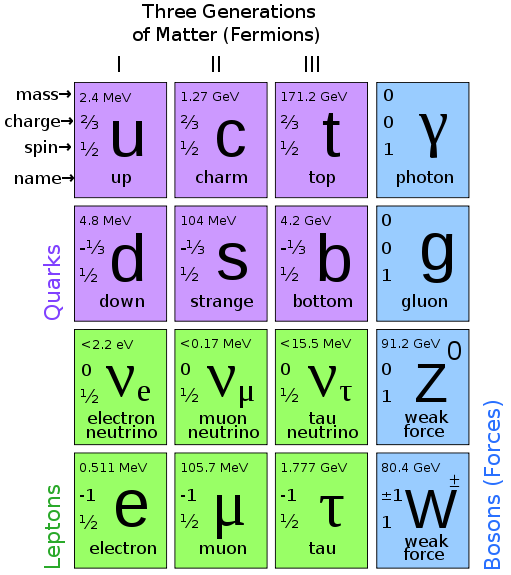
\includegraphics[width=0.6\textwidth]{imagens/standart_model.png}
\caption{O Modelo Padrão de interação entre partículas elementares. Extraído de
\cite{tese_torres}.}
\label{fig:modelo_padrao}
\end{figure}

%\newacronym[type=Simb]{bossonfoton}{\ensuremath{\gamma}}{Fóton (bóssom)} 
%\newacronym[type=Simb]{bossonZ}{\ensuremath{Z}}{Bóssom Intermediário Z} 
%\newacronym[type=Simb]{bossonW}{\ensuremath{W}}{Bóssom Intermediário W} 
%\newacronym[type=Simb]{quarku}{\ensuremath{u}}{Quark \emph{up} (partícula elementar)} 
%\newacronym[type=Simb]{quarkd}{\ensuremath{d}}{Quark \emph{down} (partícula elementar)} 
%\newacronym[type=Simb]{quarkc}{\ensuremath{c}}{Quark \emph{charm} (partícula elementar)} 
%\newacronym[type=Simb]{quarks}{\ensuremath{s}}{Quark \emph{strange} (partícula elementar)} 
%\newacronym[type=Simb]{quarkt}{\ensuremath{t}}{Quark \emph{top} (partícula elementar)} 
%\newacronym[type=Simb]{quarkb}{\ensuremath{b}}{Quark \emph{bottom} (partícula elementar)} 
%\newacronym[type=Simb]{bossong}{\ensuremath{g}}{Gluón (bóssom)} 
%\newacronym[type=Simb]{neutrinoEletron}{\ensuremath{\nu_e}}{Neutrino do elétron (partícula elementar)} 
%\newacronym[type=Simb]{neutrinoMuon}{\ensuremath{\nu_{\mu}}}{Neutrino do múon (partícula elementar)} 
%\newacronym[type=Simb]{neutrinoTaon}{\ensuremath{\nu_{\tau}}}{Neutrino do táon (partícula elementar)} 
%\newacronym[type=Simb]{eletron}{\ensuremath{e^{-}}}{Elétron (partícula elementar)} 
%\newacronym[type=Simb]{muon}{\ensuremath{\mu}}{Múon (partícula elementar)} 
%\newacronym[type=Simb]{taon}{\ensuremath{\tau}}{Táon (partícula elementar)} 

Além dessas partículas elementares, a Lei de Dirac prevê a
existência de uma antipartícula para cada partícula carregada
com a mesma massa e rotação, mas cargas invertidas. 
Quando um par de partícula e antipartícula entram em contato,
ambas de massa $m$, acabam se aniquilando e liberando sua energia de repouso $2mc$ em fótons e outras
partículas. As antipartículas são representadas através de uma barra acima dos símbolos
das partículas, ou, no caso de partículas com índices de carga, 
apenas os sinais da carga são invertidos. 
A antipartícula do elétron tem o nome de pósitron, por motivos
históricos \cite{Intro_Standard,Intro_Nuclear}. Partículas 
eletricamente neutras também possuem antipartículas, e, em alguns casos,
podem ser suas próprias antipartículas.

\subsection{Os bóssoms e as interações fundamentais}
\label{ssec:bossoms}

As interações são comunicadas através dos bóssoms, partículas elementares
de campo das interações. Cada interação tem seu
bóssom característico: o gluôn (g): interação forte; o fóton $\gamma$: interação 
eletromagnética; e os bóssoms W e Z: interação fraca.  
Os bóssoms W e Z possuem respectivamente massa de aproximadamente
80 e 90 GeV. Esse fato limita o alcance da interação fraca a cerca $10^{-3}$ fm,
uma vez que uma partícula de massa M só pode existir como parte de um estado
intermediário por tempo $\hbar/Mc^2$, viajando uma distância não maior que
$\hbar/Mc$. O bóssom W possui carga elétrica, enquanto o bóssom Z é neutro, sendo sua própria antipartícula.
O gluôn e o fóton não possuem carga, assim como massa de repouso, de forma que é esperado alcance de
interação infinito para os campos portados por essas partículas. 
Contudo, diferente do campo eletromagnético, o campo de
gluôns é confinado a um alcance de 1 fm. 
Assim, para distâncias maiores a 1 fm, a interação eletromagnética é dominante,
enquanto para distâncias menores, as interações forte e fraca também ocorrem.

\begin{table}
\centering
\resizebox{15cm}{!}{
\begin{tabular}{ccccc}
\hline
\hline
\textbf{Interação} & \textbf{Partículas Afetadas} & \textbf{Alcance} &
\textbf{Intensidade Relativa} & \textbf{Bóssoms} \\
\hline
\hline
\multirow{2}{*}{Forte} & Quarks & \multirow{2}{*}{$~10^{-15}$ m} &
\multirow{2}{*}{1} & Gluôns  \\
 & Hádrons &  &  & Mésons  \\
\hline
Eletromagnética & Partículas carregadas & $\infty$ & $10^{-2}$ & Fótons
\\
\hline
Fraca & Quarks e Léptons & $~10^{-18}$ m & $10^{-3}$ & W e Z\\
\hline
Gravitacional & Todas & $\infty$ & $10^{-39}$ & Gráviton \\
\hline
\hline
\end{tabular}
}
\caption{As quatro interações fundamentais. A intensidade relativa se dá em
relação a interação forte. Adaptado de \cite{Beiser}.}
\label{tab:interacoes}
\end{table}

Conseguiu-se unir as interações eletromagnética e fraca, chamada de interação
eletrofraca. O problema da realização de tal conexão se deu ao fato dos
bóssoms da interação fraca terem massa, fato não ocorrido para o caso da
interação eletromagnética. Para realizar essa união se mostrou que, em um
estado primitivo, uma única interação era mediada pelos quatro bóssoms sem massa.
Através de um processo chamado quebra de simetria espontânea, três dos quatro
bóssoms adquiriram massa e viraram as partículas Z e W, com a consequente
redução no alcance de interação, enquanto o quarto bóssom continuou sem massa,
tendo como consequência o alcance infinito para a parte eletromagnética da
interação original \cite{Beiser}.

\newacronym[type=Simb]{hbar}{\ensuremath{\hbar}}{constante de Planck reduzida
(\ensuremath{\frac{h}{2\pi}})} 

Os físicos esperam adicionar a interação gravitacional
através da partícula gráviton, que deverá ter rotação equivalente a 2
unidades de $\hbar$ e massa nula, entretanto não há nenhuma evidência 
experimental a favor ou contra sua existência \cite{Beiser}.
A Tabela~\ref{tab:interacoes} contêm um resumo sobre as interações
fundamentais.

\subsection{Léptons}
\label{ssec:leptons}

Os léptons podem ser subdivididos em dois grupos, 
um com massa e carga elétrica, idêntica e unitária: elétron, múon e táon; 
e outro neutro em carga e massa reduzida, estando relacionados com os léptons
carregados: neutrino do elétron, neutrino do múon e neutrino do táon. Dos
léptons carregados, o múon e o táon só diferem dos elétrons na sua massa e no
seu tempo de vida finitos, sendo o elétron o único estável.
Experimentalmente observa-se que um lépton só pode mudar para outro do seu mesmo
subgrupo, assim como um lépton só pode ser criado ou destruído em conjunto com
um anti-lépton do mesmo subgrupo. Esse fato pode ser melhor observado no
decaimento descrito por \ref{eq:muon}, onde um múon decaí em um
elétron, lépton carregado, criando ao mesmo tempo um neutrino do múon e um
antineutrino do elétron, ambos do grupo de léptons neutrinos.
Nenhum dos léptons sofrem interações com os gluôns, portadores da interação forte.
No caso do subgrupo dos léptons neutrinos, eles também não interagem com a
interação eletromagnética (fótons), 
uma vez que não têm carga, só interagindo com a interação fraca e, por esse motivo,
são de difícil detecção \cite{Intro_Nuclear,Intro_Standard}.

\begin{equation} \label{eq:muon}
\mu^{-} \rightarrow \nu_{\mu} + e^- + \bar{\nu}_{e}
\end{equation}

\subsection{Quarks e hádrons}
\label{ssec:quarks}

Os quarks possuem tanto sabores, que lhes descreve as características de massa e
carga elétrica, quanto um equivalente de carga de interação
forte, distinguido em três cores de carga forte: vermelho, verde e azul. 
Para cada geração existe um par de sabores, onde um dos constituintes do par tem
carga elétrica positiva, correspondente a $\frac{2e}{3}$,
e outro negativa, igual a $\frac{-e}{3}$. São os possíveis sabores: \emph{up}
(u) e \emph{down} (d), \emph{charm} (c) e \emph{strange} (s), \emph{top} (t) e
\emph{bottom} (b). Os quarks sofrem influência de todas as interações descritas
pelo \gls{mp}.

\newacronym[type=Abrev]{qcd}{QCD}{CromoDinâmica Quântica}

Uma dificuldade da investigação experimental dos quarks é devida aos mesmos
nunca terem sido observados isoladamente. Eles estão sempre confinados em sistemas
compostos, que se estendem a uma distância de até 1 fm, alcance máximo da interação forte. 
A \gls{qcd} é modelada na \gls{qed}, mas alterando a carga elétrica pelas cores do quark, 
prevê como os quarks e gluôns interagem para formar os hádrons. Mesmo
em colisões de altas energias os quarks se agrupam rapidamente em hádrons,
formando jatos hadrônicos \cite{Intro_Nuclear}. Esse confinamento dos quarks ocorre 
porque a interação forte é similar a uma mola, quanto mais afastados, maior é a
força de atração entre os quarks. Mas se energia suficiente for adicionada,
ao invés de um quark se liberar dos outros no hádron, a energia excedente produz
um par de quark-antiquark \cite{Beiser}.
Se dá ao nome dos sistemas compostos por quarks e gluôns de
hádrons, sendo os bárions e mésons os sistemas mais simples conhecidos. 

%\newacronym[type=Simb]{kaon}{\ensuremath{K}}{Káon (méson)} 
%\newacronym[type=Simb]{pion}{\ensuremath{\pi}}{Píon (méson mais leve existente)} 
 
Um largo espectro dos bárions podem ser explicados como uma cápsula contendo
três quarks confinados por gluôns, sendo exemplos os prótons e nêutrons. Os mésons
são compostos essencialmente por um quark e anti-quark ligados
transientemente por um gluôns. Alguns dos mésons referidos neste trabalho são
os mésons mais leves existentes, os píons: $\pi^{+}$,
$\pi^{-}$ e $\pi^{0}$, compostos respectivamente por pares $u\bar{d}$, $\bar{u}d$ e
$u\bar{u}$ ou $d\bar{d}$, e os káons, os mais leves dos mésons estranhos
(contendo quarks $s$), $K^{+}$, $K^{0}$, $K^{0}_{S}$ e $K^{0}_{L}$, 
compostos pelos sistemas $u\bar{s}$, $d\bar{s}$,
$\frac{d\bar{s}+s\bar{d}}{\sqrt{2}}$, onde a diferença do $K^{0}_{S}$ e
$K^{0}_{L}$ está no tempo de vida médio dessas partículas. 
O próton ($uud$) é o único bárion estável\footnote{Teorias atuais consideram que
o próton decai com um tempo de vida muito longo, entretanto esse valor talvez seja maior 
que o valor mínimo detectado experimentalmente, de $10^{32}$ anos. 
Para comparação, a idade do universo é de $10^{10}$ anos \cite{Beiser}.}, 
já o nêutron ($udd$), apesar de estável na estrutura atômica,
quando isolado tem vida média de 15 minutos \cite{Intro_Standard}. Finalmente, 
todos mésons são instáveis e também são bóssoms, uma vez que mediam a interação
forte entre hádrons.

\subsection{A simetria e a física}
\label{ssec:simetria}

A construção do \gls{mp} foi guiada pelos princípios 
de simetria, que podem ser divididos em diversos grupos com diferentes
propriedades matemáticas. A conexão entre a física e simetria é forte, como
demonstrado pelo Teorema de Noether, onde essencialmente, para cada simetria
continua na natureza existe uma lei de conservação correspondente. De maneira
geral, a simetria de um tipo particular existe quando uma certa operação não
altera um certo fenômeno ou objeto. A operação de simetria mais simples é a
translação no espaço, que significa que as leis da física não dependem do local
das coordenadas de origem escolhidas. Noether mostrou que essa invariância tem a
consequência da conservação do momento linear. De forma semelhante a translação
no tempo, significando que não importa a escolha de $t = 0$, resulta na
conservação de energia e a invariância de rotações no espaço, ou seja, as leis
da física são invariantes conforme a escolha da orientação do sistemas de
coordenadas, resultam na conservação de momento angular
\cite{Intro_Standard,Feynman}.

\newacronym[type=Abrev]{cp}{CP}{Carga e Paridade}

Duas leis de conservação importantes na Física de
Partículas são: Conjugação de \gls{cp}, referidas como Simetria \gls{cp}. 
A Simetria \gls{cp} diz que a física deve reagir
da mesma maneira se a partícula for alterada para sua antipartícula (C) e refletida
espacialmente (P).
Embora a Simetria \gls{cp} seja conservada para as interações forte
e eletromagnética, o mesmo não acontece para a interação fraca
\cite{Intro_Nuclear}. Esse fato pode ser uma explicação possível do
desequilíbrio de matéria e antimatéria no universo, todavia, o \gls{mp} não
prevê a violação da Simetria \gls{cp} para as interações fracas, apenas para a
interação forte em escalas de energia muito altas, de forma que são necessárias
outras fontes de violação da Simetria \gls{cp} para se estudar e expandir o modelo.
 
\subsection{O bóssom de Higgs}
\label{ssec:higgs}

Outra simetria muito importante é conhecida como a Invariância de Gauge.
Ela prevê que todos os bóssoms de rotação unitária precisam ter
massa de repouso nula, se eles forem os únicos bóssoms da teoria.
Isso é aceitável para as teorias QED e QCD, uma vez que os
fótons e gluôns não possuem massa, mas é experimentalmente contraditório
para os bóssoms Z e W. A Invariância de Gauge tem um papel ainda mais forte
quando na teoria unificada eletrofraca, onde sua consequência é que todas as
partículas contêm massa nula. Foi introduzido um mecanismo, 
por Peter Higgs em 1964, para corrigir o \gls{mp} de modo que ele atendesse
a essa formulação, conhecido como o bóssom de Higgs, portador do campo de Higgs. O bóssom de Higgs seria
uma partícula mediadora responsável de fornecer massa às partículas elementares.

A existência do bóssom de Higgs é a mais importante previsão do \gls{mp} 
ainda não verificada experimentalmente e sua busca é de máxima importância para
a Física de Partículas. Diferente dos outros bóssoms, o
bóssom de Higgs teria rotação nula \cite{Intro_Nuclear}.

\subsection{A Física Experimental de Partículas}
\label{ssec:fisexp}

O progresso da ciência tem o comprometimento entre teoria e experimento. De
acordo com Kelvin, sem se medir ou poder expressar em números o assunto tratado, 
se há apenas uma ideia inicial do conhecimento sobre o tema \cite{kelvin}. 
Na Física de Partículas Elementares, experimentos atualmente dependem
principalmente de grandes aceleradores de partículas. Outras fontes de avanço na
Física de Partículas são experimentos com raios cósmicos, estudados tanto
através de detectores na superfície terrestre como através de satélites 
\cite{nature_space_and_time}. 

De acordo com a Teoria da Relatividade, não há diferença qualitativa entre
massa e energia, essa é apenas quantitativa \cite{einstein} sendo descrita por
\ref{eq:einstein}, onde $E$ é a energia, $m_0$ a massa de repouso, e $c$ a constante que representa a
velocidade de propagação da luz no vácuo, aproximadamente $3\times10^{8}$ m/s. Ao se acelerar
partículas de pequenas massas, é possível gerar partículas com maiores massas
através das interações ocorridas durante a colisão. Experimentos em
aceleradores de partículas tiveram seu início por volta de 1930, com o
acelerador linear \emph{Crockroft-Walton} em Cambridge, Reino Unido. Esse
acelerador atingia energias de 0.7 MeV com prótons. A Tabela~\ref{tab:aceleradores} 
lista alguns dos aceleradores já construídos. Os
aceleradores podem ser lineares ou circulares, assim como de alvo fixo ou colisionadores
de feixes. Nos aceleradores de alvo fixo as partículas são aceleradas até
obterem a energia desejada e então direcionadas a um alvo estacionário. Já nos
colisionadores de feixes, as partículas são aceleradas em feixes em direções
opostas e então colididas quando a energia desejada é atingida. A aceleração é
realizada através de interação eletromagnética, de forma que apenas
partículas carregadas eletricamente são aceleradas.

\newacronym[type=Simb]{E}{\ensuremath{E}}{energia} 
\newacronym[type=Simb]{massa}{\ensuremath{m}}{massa} 
\newacronym[type=Simb]{c}{\ensuremath{c}}{constante de velocidade de propagação da luz no
vácuo} 

\begin{equation} \label{eq:einstein}
E=m_0c^2
\end{equation}

\begin{table}
\centering
\begin{tabular}{lll}
\hline \hline \hline
\textbf{Máquina} & \textbf{Partículas Colididas} & \textbf{Início-Término} \\
\hline \hline
Tevatron & p: 900 GeV & 1987 \\
(Fermilab, Batavia, Ilinóia) & $\bar{p}$: 900 GeV & \\
\hline
SLC & $e^{+}$: 50 GeV & 1989-1998 \\
(SLAC, Standford) & $e^{-}$: 50 GeV & \\
\hline
HERA & e: 30 GeV & 1992 \\
(DESY, Hamburgo) & p: 820 GeV & \\
\hline
LEP2 & $e^{+}$: 81 GeV & 1996-2000 \\
(CERN, Genebra) & $e^{-}$: 81 GeV & \\
\hline
PEP-II & $e^{+}$: 9 GeV & 1999-2008 \\
(SLAC, Standford) & $e^{-}$: 3.1 GeV & \\
\hline
LHC & p: 7 TeV & 2008 \\
(CERN, Genebra) & p: 7 TeV & \\
\hline \hline
\end{tabular}
\caption{Alguns aceleradores de partículas no mundo. Adaptado de \cite{Intro_Standard}.}
\label{tab:aceleradores}
\end{table}

\newacronym[type=Abrev]{qgp}{QGP}{Plasma de Quarks e Glúons}

Muitos aceleradores de partículas utilizam prótons pois eles são mais facilmente
acelerados, atingindo níveis mais elevados de energia. Entretanto, a
estrutura dos prótons é muito mais complexa (hádrons
compostos por quarks e gluôns) que a dos elétrons (partícula elementar), de forma que as colisões com elétrons são 
de mais fácil compreensão. Como consequência, as
descobertas normalmente são realizadas através das colisões com prótons, enquanto as medições com
maior precisão são realizadas na colisão de elétrons \cite{nature_space_and_time}.
As colisões com íons de chumbo foram introduzidas em meados dos anos 80
para se estudar o \gls{qgp} \cite{heavy_ions}.

\subsection{Além do Modelo Padrão}
\label{ssec:alem_do_mp}

O \gls{mp} ainda deixa muitas questões em aberto. Não se foi capaz, até o
momento, de adicionar o campo gravitacional ao mesmo. São necessários a
determinação de cerca de 25 a 26 parâmetros quando considerando a existência do
bóssom de Higgs. Existem realmente tal ordem de parâmetros independentes na
natureza? Ainda, experimentos astronômicos mostram que apenas 4\% do universo é
composto pela matéria conhecida no \gls{mp}, outros 23\% são de Matéria
Escura, partículas ou conglomerados massivos que não brilham ou disseminam luz,
e os 73\% restantes, grande parte da energia do universo, são de Energia Escura,
totalmente desconhecida para a ciência atual. Indo mais além, o \gls{mp} 
não explica porque o universo se consiste quase totalmente por matéria e
praticamente nenhuma antimatéria, como foi dito quando se referindo a simetria
\gls{cp}. Espera-se que o experimento LHC seja capaz de responder a essas perguntas, entre outras, 
e ajude os cientistas a resolverem as incoerências e problemas do modelo, quem sabe também reduzindo 
o número de parâmetros livres a serem determinados para um, ou dois.
\cite{nature_space_and_time,Intro_Nuclear}

\newacronym[type=Abrev]{susy}{SUSY}{teoria de SUper-SImetria}
\newacronym[type=Abrev]{gut}{GUT}{Grande Interação Unificada}

Há ainda outras duas teorias além do \gls{mp}: a \gls{susy} e a Teoria de Cordas. 
A \gls{susy} é uma expansão do \gls{mp} com um
novo principio de simetria, no qual toda partícula deve ter uma contraparte
super-simétrica, chamadas de super-partículas. Dois aspectos da \gls{susy} são
que, em primeiro lugar, ela integra as teorias separadas do \gls{mp} para formar
um papel muito mais satisfatório na procura pela \gls{gut} -- união da interação
forte com a interação eletrofraca -- e, segundo, é concebível que a Matéria Escura 
é composta de super-partículas, ainda que não tenha sido observado nenhum sinal delas 
até o momento. 

A Teoria de Cordas tem o proposto de ser a Teoria de Tudo, que uniria a
gravidade com a \gls{gut}. Nessa teoria os léptons, quarks e bóssoms não são
pontos nas quatro dimensões (x,y,z,t) do espaço-tempo, mas laços vibrantes de
cordas em um espaço de dez dimensões. Cada partícula representa um módulo de
vibração, que tem $10^{-35} m$ e por isso supostamente se
assemelham a pontos. Não se há conhecimento das seis dimensões adicionais porque
elas estão "enroladas"~para nós da mesma forma que a analogia de um papel pode
parecer como uma linha unidimensional. A Teoria de Cordas, que é muito complexa
matematicamente, incorpora as principais características da \gls{gut}, incluindo,
em particular, a \gls{susy}.

\section{O \emph{Large Hadron Collider}}
\label{sec:lhc}

\glsreset{lhc}
\newacronym[type=Simb]{ionsChumbo}{A}{íons de chumbo} 
\newacronym[type=Simb]{protons}{p}{prótons} 

Atualmente, o \gls{cern} está engajado no projeto \gls{lhc}, 
um acelerador de partículas circular de 27 km de
circunferência, situado no subsolo, dentre 50 e 175 m, custando \euro $3,03
Bi$ \cite{webLHC}. Sua parte central é um dos pontos mais frios do universo,
operando a 2 K, temperatura menor que a temperatura média do espaço. Ainda, o
vácuo desenvolvido nos seus tubos de feixes é o espaço mais vazio do Sistema
Solar \cite{closerLook}. A potência necessária para abastecer o experimento por
completo é de 180 MW, sendo estimados um consumo total de 700 GWh durante o
ano de 2009 \cite{webLHC}. 

No presente momento, ele realiza colisões de pacotes contendo $1,5\times10^{11}$ \gls{protons} 
a uma energia de 7 TeV no centro de massa, que serão expandidos a 14 TeV em 2013
\cite{webATLAS}. Para desenvolver essa energia a velocidade dos prótons será de 
$0,999999991\acrshort{c}$, percorrendo o \gls{lhc} 11000 vezes por segundo.
O \gls{lhc} também colidirá \gls{ionsChumbo}, num total de 5,5 TeV para cada par
de núcleons.

\subsection{Os objetivos do LHC}
\label{ssec:obj_lhc}

O \gls{lhc} apresenta uma oportunidade sem precedentes para conhecer os domínios da
nova física na região TeV e lançar luz sobre algumas das questões fundamentais
não resolvidas da Física das Partículas Elementares.
No caso das colisões de p-p, dentre os tópicos principais a serem testados pelo
\gls{lhc} estão \cite{hunt_for_physics}:

\newacronym[type=Abrev]{hs}{HS}{Setor Escondido}
\newacronym[type=Simb]{zprime}{Z'}{Z \emph{prime}}

\begin{itemize}
\item \textbf{Busca pelo bóssom de Higgs}: Tópico no qual este trabalho está
inserido. Se tal partícula existir, o \gls{lhc} deverá ser capaz de observá-lo;
\item \textbf{Busca pela \gls{susy}}: Algumas partículas previstas por esse
modelo, as super-partículas, 
devem ser visualizadas na região TeV;
\item \textbf{Violação \gls{cp}}: Estudo da violação da Simetria \gls{cp};
\item \textbf{Matéria escura}: Os candidatos mais relevantes vão além do \gls{mp}
para descrever a matéria escura. Um dos possíveis modelos é a \gls{susy};
\item \textbf{Física do quark \emph{top}}: Busca melhorar a compreensão da física dessa
partícula elementar, ainda não muito bem compreendida;
\item \textbf{Física do \gls{zprime}}: Estudos dos possíveis bóssoms Z adicionais; 
\item \textbf{Assinaturas visiveis do \gls{hs}}: Modelos baseados em
cordas e membranas provêm um novo setor de física, o \gls{hs}, que poderá ser
explorado pelo \gls{lhc};
\item \textbf{Provar a origem da massa dos léptons neutrinos}: Se o mecanismo que gera
suas massas estiver na região TeV, o \gls{lhc} poderá resolver essa questão;
\item \textbf{Caça por dimensões extras}: Modelo com ordens superiores de dimensões
oferecem alternativas para a \gls{susy};
\item \textbf{Busca por cordas no \gls{lhc}}: A Teria de Cordas oferece a possibilidade de
união de todas as interações conhecidas na natureza, incluindo a gravidade. Muitos
trabalhos apresentados mostram predições de cordas na escala TeV.
\end{itemize}

\subsection{A estrutura e funcionamento do LHC}
\label{ssec:struct_lhc}

\newacronym[type=Abrev]{booster}{BOOSTER}{\emph{proton synchroton BOOSTER}}
\newacronym[type=Abrev]{ps}{PS}{\emph{Proton Synchroton}}
\newacronym[type=Abrev]{sps}{SPS}{\emph{Super Proton Synchroton}}
\newacronym[type=Abrev]{linac}{LINAC}{ACelerador LINear}

Para desenvolver a altíssima energia necessária para o experimento, o \gls{cern}
utiliza outros aceleradores construídos anteriormente, acelerando
sequencialmente os pacotes de hádrons até atenderem
a energia desejada para a colisão. Na Figura \ref{fig:esquema_aceleradores} pode-se observar
o esquema de aceleração, tanto para prótons, quanto para íons de chumbo. 
No caso dos prótons, o ciclo inicia-se na extração de prótons de átomos
de hidrogênio que são acelerados no \acrshort{linac} 2, um acelerador linear,
que inicia a sequencia de aceleração, proporcionando-lhes uma energia de até 50 MeV. 
Em seguida são utilizados síncrotons, aceleradores circulares no qual as
partículas seguem a trajetórias circulares dirigidas por magnetos: \acrshort{booster} (1.4
GeV), \acrshort{ps} (25 GeV), \acrshort{sps} (450 GeV), até finalmente 
abastecer o \gls{lhc} com os pacotes de prótons. O \gls{lhc} também é um
síncroton, assim como grande parte dos aceleradores de altas energias anteriormente 
construídos \cite{lecture_slides_1,lecture_slides_2}.

\begin{figure}[h!t]
\centering
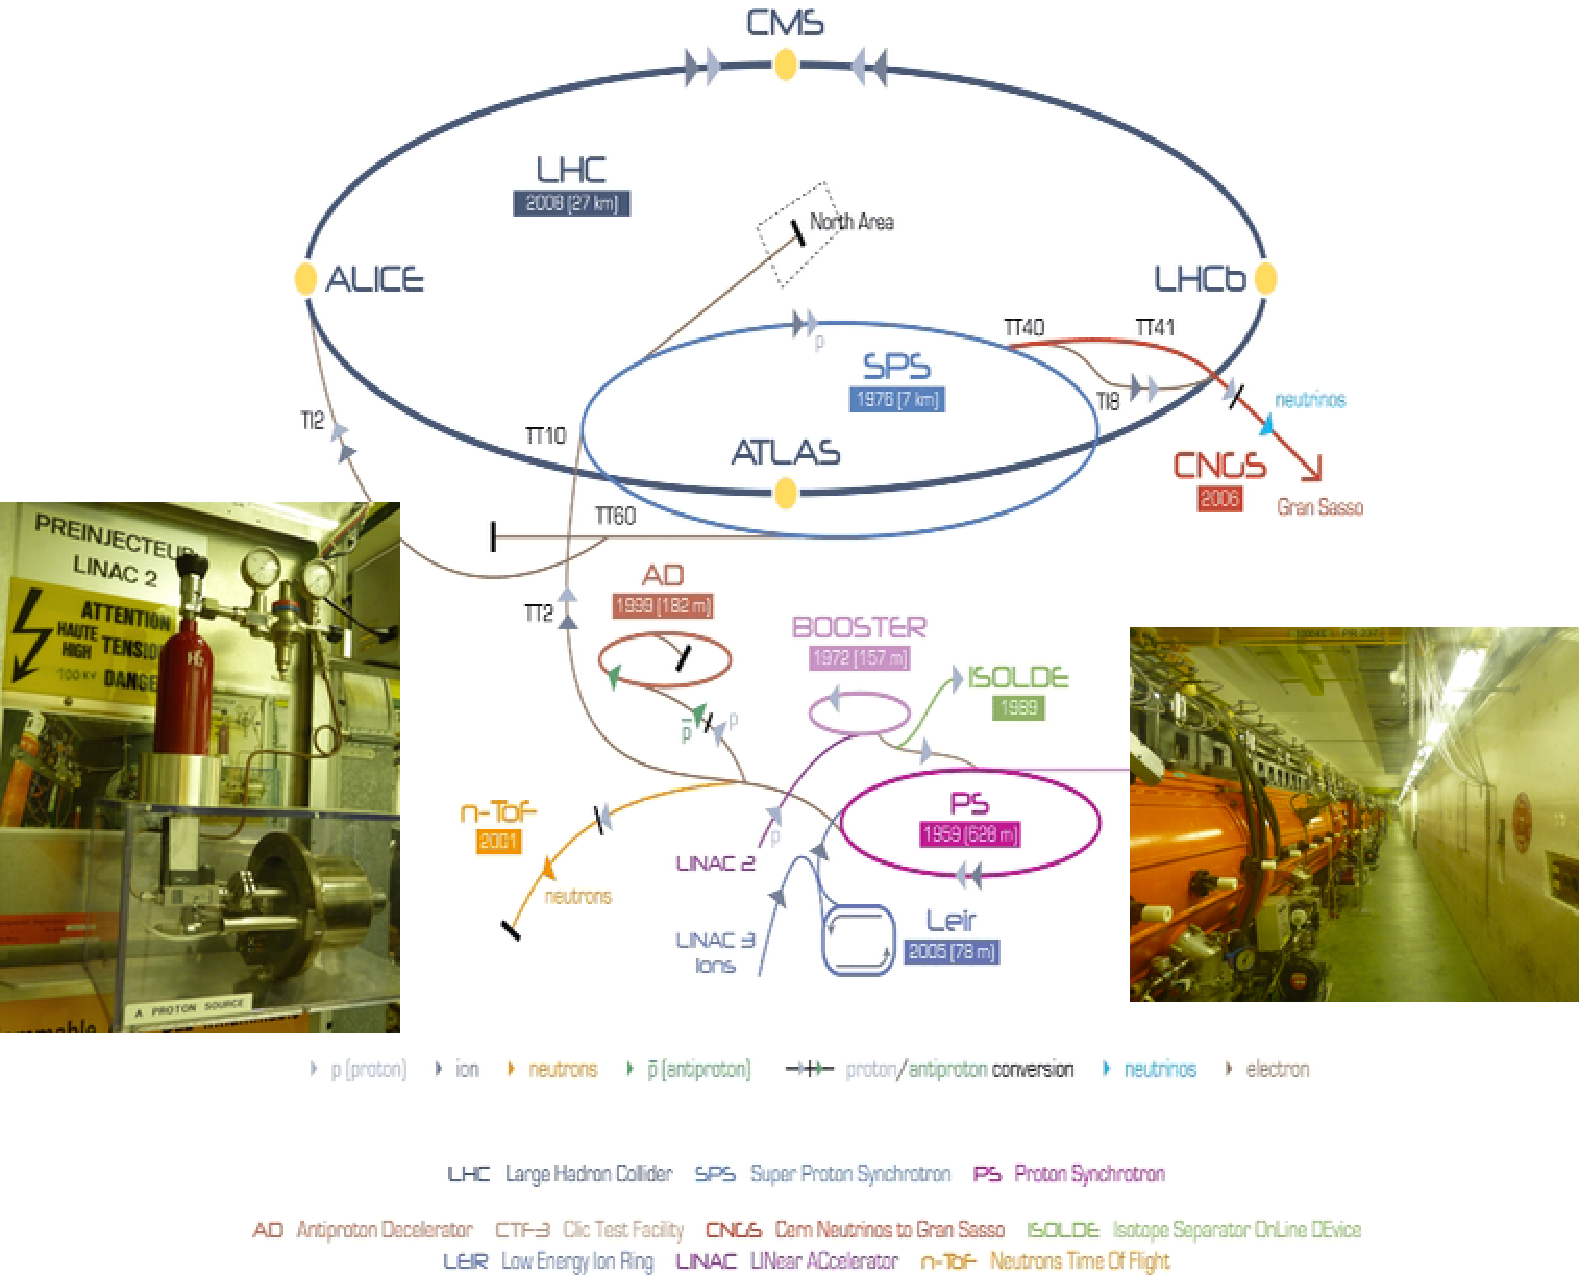
\includegraphics[width=\textwidth]{imagens/lhc_garrafa_linac2.pdf}
\caption{Os diferentes aceleradores e detectores do CERN, extraído de
\cite{cern_accelerators}. A seta cinza claro corresponde ao sentido do
deslocamento de prótons nos aceleradores. A esquerda, foto da garrafa
de hidrogênio de onde são retirados os prótons, e na direita foto do LINAC 2.}
\label{fig:esquema_aceleradores}
\end{figure}

\newacronym[type=Abrev]{alice}{ALICE}{\emph{A Large Ion Collider Experiment}}
\newacronym[type=Abrev]{lhcb}{LHCb}{\emph{Large Hadron Collider beauty experiment}}
\newacronym[type=Abrev]{totem}{TOTEM}{\emph{Total Cross Section, Elastic
Scattering and Diffraction Dissociation}}
\newacronym[type=Abrev]{cms}{CMS}{\emph{Compact Muon Sollenoid}}
\newacronym[type=Abrev]{moedal}{MoEDAL}{\emph{the Monopole and Exotics Detector At the
\acrshort{lhc}}}
\newacronym[type=Abrev]{lhcf}{LHCf}{\emph{\acrshort{lhc} forward}}

\newacronym[type=Abrev]{fodo}{FODO}{\emph{FOcusing DefOcusing}}
\newacronym[type=Abrev]{rf}{RF}{\emph{Radio Frequency}}
\newacronym[type=Abrev,\glslongpluralkey={Pontos de Inserção},
\glsshortpluralkey={IPs}]{ip}{IP}{Ponto de Inserção}

O \gls{lhc} não é uma circunferência perfeita, sendo dividido em octantes, 
contendo dois arcos e um trecho reto, iniciando e terminando no ponto
intermediário de arcos sucessivos. Os arcos medem cerca de 2,45 km,
cotendo 23 células em estrutura \gls{fodo}, que serão detalhadas
posteriormente nesta seção. 
Cada trecho reto tem 528 m e são utilizados como \glspl{ip},
seja para um experimento ou para uma utilidade. A parte
compreendida entre dois \glspl{ip} é chamada de setor. A 
Figura~\ref{fig:esquema_lhc} contêm um esboço da estrutura do \gls{lhc}, assim
como as utilizações de seus \glspl{ip}.

\begin{figure}[h!t]
\centering
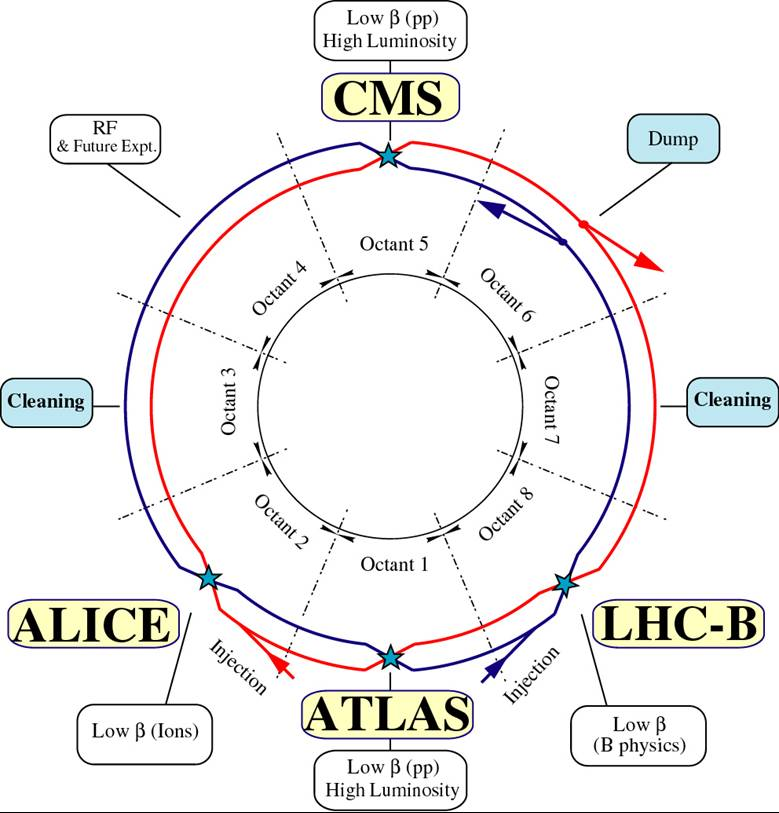
\includegraphics[width=.6\textwidth]{imagens/lhc-schematic.png}
\caption{Esboço esquemático do LHC, extraído de
\cite{webLHC}. Os diversos octantes do LHC, contendo os pontos de inserção 
com suas respectivas funcionalidades e experimentos.
O anel 1, em vermelho, gira no sentido horário, enquanto o anel
2, em azul, gira no sentido antihorário.}
\label{fig:esquema_lhc}
\end{figure}

No total existem quatro \glspl{ip} experimentais, nos quais os feixes são
direcionados para a colisão. Os dois \glspl{ip} para
os experimentos de alta luminosidade estão localizadas em seções diametrais
opostas, sendo os mesmos os detectores \acrshort{atlas}, no \gls{ip}1, e
\acrshort{cms}, \gls{ip}5. 
Os outros dois pontos são para os detectores \acrshort{alice} e
\acrshort{lhcb}, localizados respectivamente no \gls{ip}2 e \gls{ip}8. Nesses últimos
pontos também estão localizados os sistemas de injeções para os feixes, que
alimentam os anéis dos feixes do \gls{lhc} 
com os pacotes de hádrons, sendo o anel 1 o feixe em rotação horária alimentado
pelo \gls{ip}2, e o anel 2 o 
feixe em rotação anti-horária alimentado pelo \gls{ip}8. 
A injeção ocorre no plano vertical, com os feixes
vindo por baixo do plano de \gls{lhc}. 

Apenas uma fração de $10^{-6}$ dos feixes é capaz de causar
danos aos magnetos super-condutores, ou mesmo destruir partes do detector\footnote{A 
energia armazenada nos feixes, 360 MJ, é capaz de derreter uma tonelada 
de cobre \cite{closerLook,lhc_design}.}. Nos \gls{ip}3 e \gls{ip}7 estão localizados 
dois sistemas de colimação, fazendo a proteção 
do acelerador contra as perdas inevitáveis e limpando os feixes de
qualquer irregularidade. A diferença entre os pontos \gls{ip}3 e \gls{ip}7 está
em duas limpezas adicionais realizadas nesses pontos. No \gls{ip}3 se
encontra um sistema para a limpeza de momento de ambos os feixes, oscilação
gerada pelo sistema \acrshort{rf}. Já no \gls{ip}7 se encontra um sistema de
limpeza das oscilações \emph{betatron}. Ambos efeitos serão descritos com
maiores detalhes a seguir. Essas são as áreas mais radioativas do \gls{lhc} 
\cite{lhc_design}.

Conforme o acontecimento de colisões, o número de hádrons nos pacotes irá se
deteriorar, no caso de prótons o tempo de vida médio é de 10 h, de modo que é necessário ter um 
sistema de remoção para os pacotes inúteis. Com esse objetivo existe um Sistema de Remoção no
\gls{ip}6, contendo um sistema independente para cada feixe. 
A sua função é extrair rapidamente os pacotes de cada um dos anéis do \gls{lhc}, evitando quaisquer
perdas de outros pacotes e transportá-los até um material
absorvedor. Devido ao poder destrutivo dos feixes, o Sistema de Remoção deve ter
altíssima confiabilidade, que condicionaram sua concepção.

\newacronym[type=Simb]{frf}{\ensuremath{f_{RF}}}{frequência do sistema RF} 
\newacronym[type=Simb]{frev}{\ensuremath{f_{rev}}}{frequência de revolução} 

No \gls{ip}4 está localizado dois (um para cada feixe) sistemas independentes de \gls{rf}, 
que irão realizar a aceleração das partículas no \gls{lhc}. A
aceleração é feita nas cavidades \gls{rf}, onde são geradas tensões oscilantes
com a \gls{frf} de 400 MHz no sentido longitudinal, criando uma
tensão acelerante. São utilizadas 8 células individuais de cavidades por feixe,
agrupando 4 células em um mesmo criostato que irá operar numa temperatura de 4,5 K.
Para que uma partícula sempre encontre uma tensão
acelerante elas precisam estar separadas por uma fase fixa, no caso da
\gls{frf}: 25 ns. O pré-injetor \acrshort{ps} é o encarregado de
realizar tal espaçamento entre as partículas. Uma partícula que está exatamente
sincronizada com a \gls{frf} é chamada de partícula síncrona, entretanto,
nem todas partículas vão estar sincronizadas. Supondo uma partícula assíncrona com maior
energia que a partícula síncrona, podem ocorrer dois efeitos dependendo da faixa
de energia da partícula síncrona (o efeito análogo oposto irá 
ocorrer caso a partícula assíncrona tenha menor energia que a síncrona):

\begin{enumerate}
\item Se a energia das partículas sincronas for baixa, irá predominar 
o aumento da velocidade da partícula assíncrona, de forma que a mesma irá
atingir a cavidade \gls{rf} \textit{antes} daquela em sincronismo.
\item Já em altas energias, irá predominar o aumento da órbita da partícula
assíncrona de forma que a mesma irá atingir a cavidade \textit{depois}
daquela em sincronismo.
\end{enumerate}

\newacronym[type=Simb]{phaseinc}{\ensuremath{\Phi_{s}}}{fase de sincronismo} 
\begin{figure}[h!t]
\centering
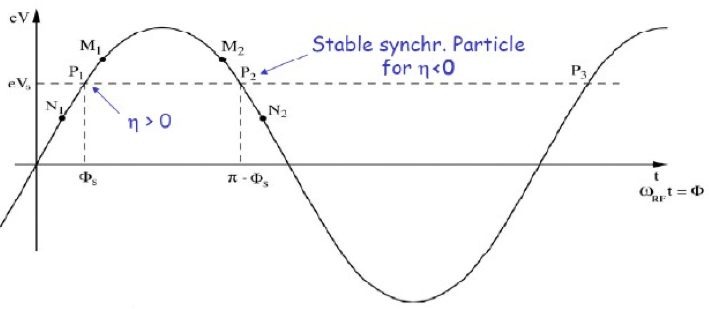
\includegraphics[width=.7\textwidth]{imagens/estabilidade_fase.png}
\caption{Estabilidade das partículas no feixe dos síncrotons. No eixo y, a
aceleração aplicada pela cavidade RF em função da fase das partículas. 
A fase de estabilidade P1 ocorre para baixas energias, e P2 para altas energias. 
Extraído de \cite{lecture_slides_1}.}
\label{fig:est_sinc}
\end{figure}

Como ilustrado na Figura~\ref{fig:est_sinc}, a \gls{phaseinc} se compreende entre
$0^\circ$ e $90^\circ$ quando o primeiro efeito é predominante, uma vez que uma partículas 
atrasadas (maior fase) irão receber maior aceleração, 
e partículas adiantadas (menor fase) irão receber menor aceleração. Para o
segundo efeito, se obtêm estabilidade entre $90^\circ<\gls{phaseinc}<180^\circ$.
Em algum momento as partículas irão atingir a energia de transição, energia no
qual ocorrerá a escursão de $\gls{phaseinc}$ para $180^\circ - \gls{phaseinc}$. Pequenas
diferenças de fase criam um efeito de oscilação harmônica em torno dos pontos de
sincronismo, significando que a distribuição das partículas não é uniforme, mas
formada por aglomerados de partículas chamados de pacotes. Um total de 35640 
possíveis pontos de estabilidade podem ser preenchidos por pacotes, determinado
pela fração entre a \gls{frf} e \gls{frev}. 
Por outro lado, mesmo que o Sistema de Remoção seja
veloz, ele ainda exige um tempo considerável para realizar sua função, assim, o
número de pacotes no \gls{lhc} é de 2808 para cada feixe
\cite{closerLook,lhc_design,lecture_slides_1,lecture_slides_2}.

\newacronym[type=Abrev]{mq}{MQ}{Quadripólos Principais} 
\newacronym[type=Abrev]{mb}{MB}{Dipólos Principais} 

Os \gls{mb} do \gls{lhc} são os responsáveis por realizar a defleção
das partículas.  São necessários magnétos fortes para curvar os feixes de altas
energias, sendo, na verdade, a capacidade dos mesmos o fator que limita a energia
dos feixes. Por isso, a tecnologia utilizada neles está no limiar da ciência
atual, contando com super-condutores resfriados a 2 K, que criaram campos
magnéticos de até 8 T.

Enquanto isso, os \gls{mq} são responsáveis por concentrar os
feixes em torno da trajetória nominal. Os quadripólos tem a propriedade de
focar as partículas em um plano, e desfocar no plano perpendicular, sendo
possível modificar o plano de enfoque ao rotacionar o quadripolo em $90^\circ$,
ver Figuras~\ref{fig:foco_eixo_x} e~\ref{fig:foco_eixo_y}. 
Para realizar a concentração dos feixes, é
utilizada o estrutura \gls{fodo}. Pode-se fazer uma analogia a óptica para tal
estrutura, como na Figura~\ref{fig:esq_fodo}, de forma que são 
utilizados quadripólos focando e desfocando as partículas. Essa estrutura cria um efeito
chamado de oscilações \emph{betatron}, onde as partículas oscilam em torno da
trajetória nominal.

\begin{figure}[ht!]
    \label{fig:quadripolos}
    \begin{center}
%
        \subfigure[Quadripólos focando as partículas no eixo \textbf{x}.]{%
            \label{fig:foco_eixo_x}
            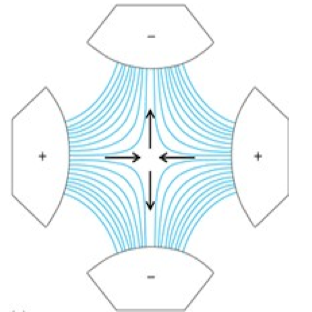
\includegraphics[width=0.3\textwidth]{imagens/quadripolo_1.png}
        } \hspace{0.1\textwidth}
        \subfigure[Quadripólos focando as partículas no eixo \textbf{y}.]{%
            \label{fig:foco_eixo_y}
            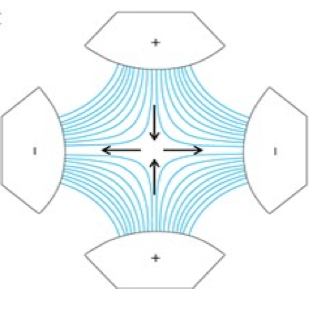
\includegraphics[width=0.3\textwidth]{imagens/quadripolo_2.png}
        }\\ %  ------- End of the first row ----------------------%
        \subfigure[A estrutura FODO utilizado para concentrar as partículas. ]{%
            \label{fig:esq_fodo}
            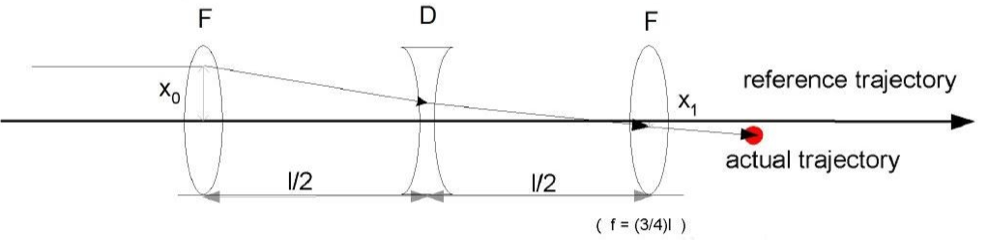
\includegraphics[width=\textwidth]{imagens/betatron.png}
        }%
        %\subfigure[Caption of Fourth Figure]{%
        %    \label{fig:fourth}
        %    \includegraphics[width=0.4\textwidth]{FourthFigure}
        %}
%
    \end{center}
    \caption{%
        A utilização do magneto de quadripólos na concentração das partículas em
      torno da trajetória nominal e a estrutura FODO. Figuras extraídas de 
      \cite{lecture_slides_1}.
     }%
\end{figure}


A estrutura \gls{fodo} utilizada nos arcos do \gls{lhc} pode ser observada na
Figura~\ref{fig:fodo_lhc}. Nela se encontram os já citados \gls{mb} e
\gls{mq}, assim como outros magnétos que realizam correções de maiores ordem,
como por exemplo a correção devido ao efeito da gravidade no feixe. 

\begin{figure}[h!t]
\centering
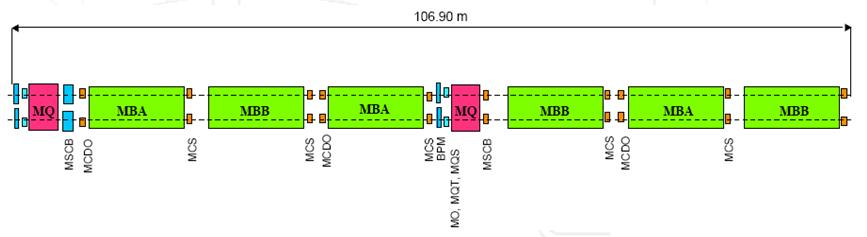
\includegraphics[width=\textwidth]{imagens/fodo_lhc.jpg}
\caption{A estrutura FODO do LHC. Extraído de \cite{closerLook}.}
\label{fig:fodo_lhc}
\end{figure}

Nas transições de arcos com os trechos retos são inseridos 
Supressores de Dispersão, totalizando 16 deles, cuja as funções são
\cite{lhc_design}:

\begin{itemize}
\item Adaptar a órbita de referência do \gls{lhc} com a geometria do túnel;
\item Cancelar a dispersão horizontal nos arcos, geradas tanto pela descontinuidade na
separação / recombinação dos dipolos magnéticos, como pelos desvios causados nas
colisões;
\item Ajudar na combinação entre a óptica de inserção com a solução períodica nos arcos.
\end{itemize}

Finalmente, \emph{Low Triplets}, grupo de quadripólos especiais, são utilizados antes dos
\glspl{ip} experimentais, afim de concentrar ao máximo os feixes nos pontos de
colisão. Eles são os responsáveis pela alta luminosidade durante a colisão.

\subsection{Detectores do LHC}
\label{ssec:lhc_detectores}

Uma vez atingido a energia desejada para as colisões dos hádrons no \gls{lhc}, 
os pacotes serão então colididos nos \glspl{ip} experimentais. Neles são colocados detectores
para realizar a medição dos eventos de colisão ocorridos, onde o   
\gls{lhc} conta com distintos detectores, cada um deles projetado 
de modo a explorar com maior eficiência a diversa física gerada
durante as colisões. 

\glsreset{atlas}

Os detectores são experimentos fundados independentes do \gls{cern}. O
\gls{cern} é um membro da colaboração de cada um dos experimentos e contribui com parte do
orçamento de cada um dos experimentos. São utilizados quatro detectores de maior
escala: \acrshort{atlas} (14\% do material contribuído pelo \gls{cern}),
\acrshort{cms} (20\%), \acrshort{alice} (16\%) e \acrshort{lhcb} (20\%); e três de menor escala:
\acrshort{totem}, \acrshort{lhcf} e \acrshort{moedal}. O trabalho atual está definido no
escopo da colaboração do detector \acrshort{atlas} (seção~\ref{sec:ATLAS}). 
Uma descrição breve deles será realizada a seguir
\cite{lecture_slides_1,lecture_slides_2,closerLook}: 
\begin{itemize}
\item \textbf{\gls{atlas}} e \textbf{\gls{cms}} são de propósito geral, ou seja, são capazes de estudar 
diversos fenômenos físicos. O fato de existirem dois detectores projetados de forma
diferente, mas para o mesmo fim, é importante para que as descobertas físicas
sejam confirmadas por ambos experimentos, garantindo que elas não sejam
tendênciosas. Algumas das diferenças mais importantes entre os dois detectores são:
\begin{enumerate}
\item O calorímetro eletrogmanético do \gls{cms} é composto por cristais de
$\text{PbWO}_4$, enquanto o
\gls{atlas} projetou o seu calorímetro com argônio líquido;
\item O sistema detector de traços do \gls{cms} é totalmente composto de
silicone, enquanto o do \gls{atlas} é composto desse material apenas na parte mais
interna. Ainda, a segmentação no \gls{cms} é maior, o que será importante em
maiores luminosidades.
Por outro lado, todo esse silicone e serviços associados (cabos, resfriamento
etc) poderá causar a interação das partículas antes delas atingirem o calorímetro,
podendo degradar os benefícios do calorímetro eletromagnético de $\text{PbWO}_4$;
\item O solenóide do \gls{atlas} está localizado dentro do seu sistema de
calorimetria, sendo a configuração padrão, já o oposto ocorre para o \gls{cms}.
O solenóide do \gls{cms} gera 4T e é o maior do mundo.
\item O \gls{atlas} tem magnétos toroidais que são utilizados como um
espectômetro separado para mûons. O \gls{cms} não possui tal
sistema, entretanto, ele utiliza medições independentes do momento dos mûons
usando o campo magnético no laço de retorno de seu solenóide;
\end{enumerate}
\item \textbf{\gls{lhcb}} é um detector especializado no estudo do méson B com o
intuito de compreender a Violação \gls{cp} e a diferença de matéria e
anti-matéria. O experimento irá melhorar resultados anteriores tanto
qualitativamente quanto quantitativamente, explorando grande parte dos
diferentes mésons B produzidos no \gls{lhc}. Eles deverão surgir de colisões que
irão se propagar próximas a direção do feixe, de forma que o \gls{lhcb} 
é um detector projetado para medir partículas com pequenos valores angulares de
colisão.
\item \textbf{\gls{alice}}, por sua vez, estudará o \gls{qgp} que será formado
enquando o \gls{lhc} fizer colisões de íons de chumbo. Esse detector é composto
principalmente de dois componentes, a parte central composta de detectores dedicados
a estudar sinais hadrônicos e elétrons, e o espêctometro de mûons avançado,
dedicado a estudar o comportamento de quarks na matéria condensada.
\item \textbf{\gls{lhcf}} se situa na mesma caverna do \gls{atlas}, a cerca de
140 m do ponto de interação para ambos lados. Ele estuda a seção de choque (ver
\ref{ssec:lhc_lum_choque}) de produção de
partículas neutras na região dianteira das colisões, utilizando
partículas que não chegaram a colir no ponto de colisão, 
mas foram desviadas. Esse estudo irá ajudar a compreender o desenvolvimento de
chuveiros cósmicos induzidos por raios cósmicos de altas energias.
\item \textbf{\gls{totem}} está instalado em um tunel separado aproximadamente a
200 m do \gls{cms}. Ele mede a seção de choque total de colisões p-p, e estuda colisões 
elásticas e difrativas no \gls{lhc}. 
\item \textbf{\gls{moedal}} é o mais novo dos experimentos do \gls{lhc},
aprovado em dezembro de 2009. Embora barato e fácil de instalar seu potêncial
de explorar física é grande, sendo instalado na caverna do \gls{lhcb}. 
Ele irá buscar evidências de partículas hipotéticas, como partículas estáveis de monopólo
magnético e outras partículas estáveis super-simétricas e massivas, através de
cauterizações no plástico do detector.
\end{itemize}


\subsection{Das colisões, seus tipos e parâmetros relacionados}
\label{ssec:lhc_lum_choque}

Nesta subseção serão apresentados parâmetros importantes envolvidos nas
colisões. Iniciará-se com uma breve introdução a cinemática das colisões e as 
coordenadas utilizadas. A taxa de colisão é
afetada por dois parâmetros, a luminosidade e a seção de choque, que serão
posteriormente descritos com maiores detalhes. Em seguida serão
apresentados os tipos de colisões, divididos de acordo com a intensidade da
alteração da estrutura dos hádrons em interação. Por fim, serão tratados
fenômenos envolvidos durante as colisões que irão afetar a busca por física 
de interesse, sendo eles o Empilhamento e os Eventos Adjacentes. 

\subsubsection{A cinemática das colisões}

Ainda que não seja o objetivo do trabalho, um breve resumo da cinemática
relativística envolvida nas interações de partículas ajudará a entender algumas
das variáveis comumente utilizadas. 
Como o trabalho está englobado no experimento \gls{atlas}, irá considerar o 
eixe de coordenadas adotado para o \gls{ip}1, ponto de inserção do mesmo. 

\newacronym[type=Simb]{theta}{\ensuremath{\theta}}{ângulo polar} 
\newacronym[type=Simb]{phi}{\ensuremath{\phi}}{ângulo azimutal} 
\newacronym[type=Simb]{z}{\ensuremath{z}}{eixo de propagação do feixe} 
\newacronym[type=Simb]{y}{\ensuremath{y}}{rapidez} 
\newacronym[type=Simb]{mom}{\ensuremath{\vec{p}}}{momento linear} 
\newacronym[type=Simb]{eta}{\ensuremath{\eta}}{pseudorrapidez} 
\newacronym[type=Simb]{pt}{\ensuremath{p_T}}{momento transverso} 
\newacronym[type=Simb]{pl}{\ensuremath{p_L}}{momento longitudinal} 
\newacronym[type=Simb]{mt}{\ensuremath{m_T}}{massa transversa} 
\newacronym[type=Simb]{Et}{\ensuremath{E_T}}{energia transversa} 

Normalmente se utilizam coordenadas cilindricas ($p,\theta,\phi$), uma vez que 
essa é a geometria das colisões.
Seus eixos definidos em coordenadas retangulares estão dispostos 
na Figura~\ref{fig:atlas_p1_coord}, sendo o eixo \emph{z} a direção do feixe com
o lado positivo na direção do \gls{ip}8, o eixo
\emph{x} aponta na direção do centro do anel do \gls{lhc} e o eixo \emph{y}
aponta para a superfície.  
As transformações para coordenadas cilíndricas
são bem conhecidas e realizadas através de \ref{eq:transf_cil}.  
A física é simétrica em relação ao \gls{phi}, 
mas há correlação entre o
tipo de colisão com o \gls{theta}, onde geralmente quanto mais forte a
interação ocorrida durante a colisão mais próximo de $90^\circ$ será esse
ângulo. O plano transverso é definido 
pelo corte transversal à direção de propagação do feixe, sendo o plano-xy do
sistema de coordenadas descrito, e a componente restante, paralela a direção de
propagação do feixe ($z$), é chamada de componente longitudinal.

\begin{figure}[h!t]
\centering
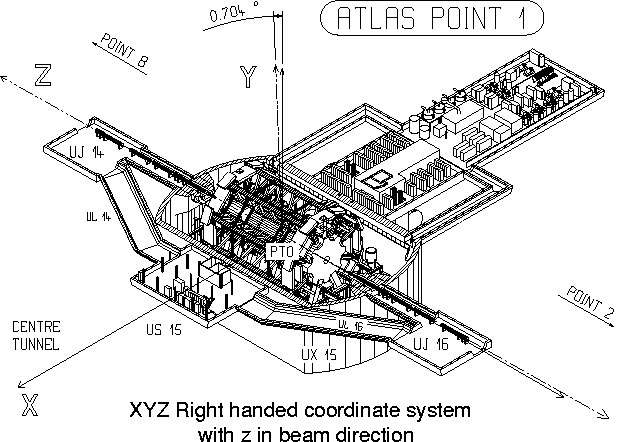
\includegraphics[width=0.7\textwidth]{imagens/atlas_p1_coord.png}
\caption{O Sistema de Coordenadas adotado para o IP1, ponto de inserção do
experimento ATLAS. Extraído de \cite{tese_torres}.}
\label{fig:atlas_p1_coord}
\end{figure}

\begin{subequations}\label{eq:transf_cil}
\begin{equation}\label{eq:transf_phi}
\phi = arctan\left( \frac{x}{y} \right) \\
\end{equation}
\begin{equation}\label{eq:transf_theta}
\theta = arctan\left( \frac{x}{z} \right) 
\end{equation}
\end{subequations}

Estando interessado no momento das partículas
produzidas, afim de se evitar as transformações de Lorentz, se faz mão de dois
parâmetros. Um deles, a \gls{y}, foi introduzido pela métrica de Minkowski
\cite{schlippe} e está definido na equação~\ref{eq:rapidez}.
O outro é o \gls{pt}, a projeção do momento no plano
transverso, dado pela ~\ref{eq:pt}. 
Esses parâmetros são invariantes as transformações relativisticas 
longitudinais. O \gls{pl}, que não é conservado nas colisões entre hádrons por
esses não serem partículas ponto, pode ser obtido através
de~\ref{eq:pl}. Outras duas variáveis que também
são projetadas no plano transverso são a \gls{mt} e \gls{Et}, obtidas através das
relações~\ref{eq:mt} e \ref{eq:Et}.

\begin{equation}\label{eq:rapidez}
y = \frac{1}{2}ln\left(\frac{E+p_z}{E-p_z}\right)
\end{equation}

\begin{subequations}\label{eq:proj_transv}
\begin{equation}\label{eq:pt}
p_T = p sen ( \theta ) = \sqrt{(p_x^2 + p_y^2)}
\end{equation}
\begin{equation}\label{eq:mt}
m_T = m^2 + p_T
\end{equation}
\begin{equation}\label{eq:Et}
E_T = E sen ( \theta )
\end{equation}
\end{subequations}

\begin{equation}\label{eq:pl}
p_L = p_z = m_T senh ( y )
\end{equation}

Os detectores absorvem a energia total (E) de grande parte das partículas
geradas nas colisões através de seus calorímetros, 
estando a mesma relacionada com a \gls{mt} por \ref{eq:etot}. Entretanto, na física de 
altas energias algumas aproximações podem
ser feitas de modo a facilitar a manipulação dos parâmetros. No caso ultrarrelativístico (quando $p \gg
m$) a rapidez se aproxima da \gls{eta}, parâmetro relacionado a \gls{theta}
através das equações \ref{eq:eta} \cite{pdg_book}.
Ainda, nesses casos a \gls{mt} tende a se aproximar de
\gls{pt}, e a energia total das partículas é predominantemente dado
pelo momento das partículas. Desta forma, ao se projetar a energia absorvida
pelo calorímetro no plano tranverso obtêm-se diretamente o \gls{pt} das
partículas, equação~\ref{eq:e_pt}, obtida aplicando as relações \ref{eq:eta} em \ref{eq:etot}.

\begin{equation}\label{eq:etot}
E = m_{T}cosh(y) \approx m_{T}cosh(\eta) \approx p_{T}cosh(\eta)
\end{equation}
\begin{equation}\label{eq:eta}
\eta = -ln \left( tan\left( \frac{\theta}{2} \right) \right) \;,\; senh(\eta) =
cot(\theta) \;,\;  cosh(\eta) = 1 / sen(\theta) \;,\; tanh(\eta) = cos(\theta) 
\end{equation}
\begin{equation}\label{eq:e_pt}
p_t \approx \frac{E}{sen(\theta)}
\end{equation}


\subsubsection{Luminosidade e Seção de Choque}
\newacronym[type=Simb]{densI}{\ensuremath{\vec{J}}}{densidade de corrente} 
\newacronym[type=Simb]{f}{\ensuremath{f}}{frequência} 
\newacronym[type=Simb]{crossSeq}{\ensuremath{\sigma}}{seção de choque} 

\newacronym[type=Simb]{lum}{\ensuremath{L}}{luminosidade} 
\label{sssec:Lum_Crosseq}
Tão importante quanto obter altas energias, é obter alta
\gls{lum}, um indicador da concentração 
de partículas no ponto de colisão, parâmetro similar a \gls{densI} 
utilizado na engenharia elétrica. A luminosidade, de maneira
simplificada, pode ser definida por
\ref{eq:luminosidade}. Nela a \gls{f} de cruzamento entre feixes
é de 40 MHz, $n$ é o número de feixes, 
$N_i$ equivale ao número de prótons em
cada pacote, correspondentes a $1.5\times10^{11}$ no início de uma
temporada\footnote{Traduzido do inglês \emph{run}.} de colisão nominal, e,
finalmente, o termo A é a área dada pela seção transversal do feixe, 
de 64 microns (aproximadamente um fio de cabelo) no ponto de colisão
\cite{webLHC}. No \gls{lhc}, serão atingidas nos experimentos de maior luminosidade 
valores de $10^{34}cm^{-2}s^{-1}$.


\begin{equation} \label{eq:luminosidade}
\gls{lum}=fn\frac{N_1 N_2}{A}
\end{equation}

\begin{equation}
R = \gls{lum} \times \sigma
\label{eq:taxa_colisao}
\end{equation}

A taxa de colisões é diretamente proporcional a luminosidade e a \gls{crossSeq}, 
definida por \ref{eq:taxa_colisao}. A seção de choque, expressa em mbarn, 
é determinada experimentalmente e indica a probabilidade de ocorrência de uma colisão. 
A Figura~\ref{fig:lum_cross} mostra a relação da seção de choque com a energia
da colisão no centro de massa, sendo possível visualizar que a probabilidade 
de ocorrer um evento de colisão de interesse, como a geração do
bóssom de Higgs com 150GeV, é maior no \gls{lhc} 
que aquele no Tevatron devido a diferença de energia nos dois aceleradores.
Já a luminosidade é determinada pelo projeto e a tecnologia utilizada no 
acelerador, sendo possível através do mesmo elevar a taxa de eventos, o que
explica, assim, a busca por elevadas luminosidades.

\begin{figure}[h!t]
\centering
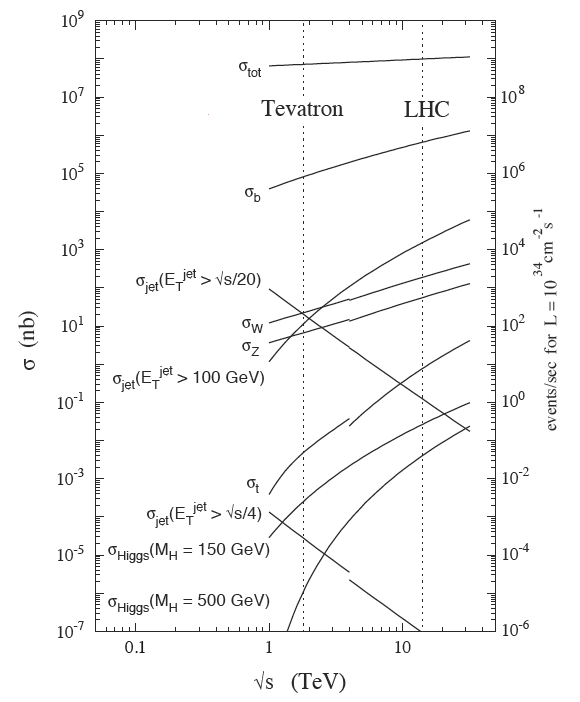
\includegraphics[width=.7\textwidth]{imagens/Lum_cross.png}
\caption{
A seção de choque, na escala a esquerda, em função da energia de colisão no
centro de massa. A escala a direita contêm a taxa de eventos por segundo 
para a luminosidade de $10^{34}cm^{-2}s^{-1}$. 
Extraído de \cite{ATLAS_HLT_DAQ}.}
\label{fig:lum_cross}
\end{figure}

\newacronym[type=Abrev,\glslongpluralkey={Colisões Elásticas}
]{el}{EL}{Colisão Elástica} 
\newacronym[type=Abrev,\glslongpluralkey={Colisões Inelásticas}
]{in}{IN}{Colisão Inelástica}
\newacronym[type=Abrev]{ds}{DS}{Colisão Difrativa Simples}
\newacronym[type=Abrev]{dd}{DD}{Colisão Difrativa Dupla}
\newacronym[type=Abrev,\glslongpluralkey={Colisões Não
Difrativas}]{nd}{ND}{Colisão Não Difrativa}
\newacronym[type=Abrev,\glslongpluralkey={Colisões Não Difrativas
Suaves}]{nds}{NDS}{Colisão Não Difrativa Suave}
\newacronym[type=Abrev,\glslongpluralkey={Colisões Não Difrativas
Rígidas}]{ndr}{NDR}{Colisão Não Difrativa Rígida}


\subsubsection{Tipos de colisão}
\label{sssec:tipos_col}

\begin{equation}
\sigma_{tot} =  \sigma_{EL} + \overbrace{\sigma_{DS} + \sigma_{DD} +
\underbrace{\sigma_{NDS}+\sigma_{NDR}}_{\sigma_{ND}}}^{\sigma_{IN}}
\label{eq:secao_choque}
\end{equation}

\begin{figure}[ht!]
    \label{fig:colisoes}
    \begin{center}
%
        \subfigure[Colisões Elásticas (EL).]{%
            \label{fig:col_el}
            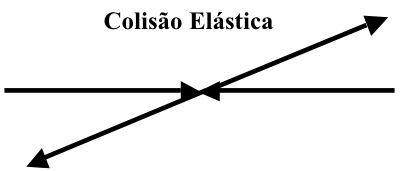
\includegraphics[width=0.3\textwidth]{imagens/col_el.png}
        } \hspace{0.005\textwidth}
        \subfigure[Colisões de Difração Simples (DS).]{%
            \label{fig:col_ds}
            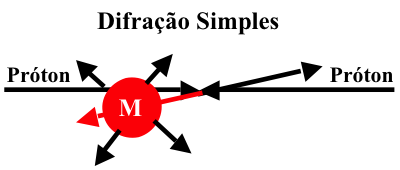
\includegraphics[width=0.3\textwidth]{imagens/col_ds.png}
        } \hspace{0.005\textwidth}
        \subfigure[Colisões de Difração Duplas (DD).]{%
            \label{fig:col_dd}
            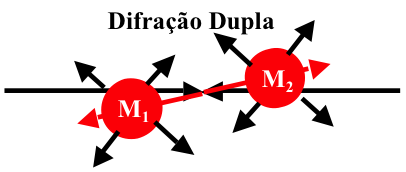
\includegraphics[width=0.3\textwidth]{imagens/col_dd.png}
        }\\ %  ------- End of the first row ----------------------% 
        \subfigure[Colisões Inelásticas Não Difrativas Suaves (NDS) ]{%
            \label{fig:col_cs}
            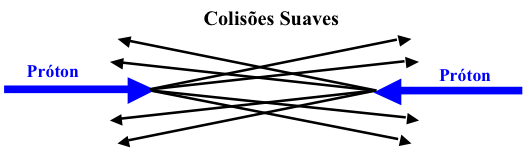
\includegraphics[width=0.45\textwidth]{imagens/col_cs.png}
        }
        \subfigure[Colisões Inelásticas Não Difrativas Rígidas (NDR)]{%
            \label{fig:col_cr}
            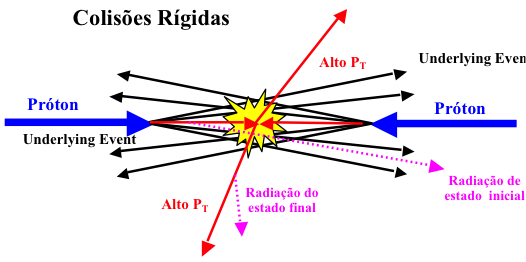
\includegraphics[width=0.45\textwidth]{imagens/col_cr.png}
        }
%
    \end{center}
    \caption{%
       As diversas colisões possíveis na física de altas energias. Adaptado de
\cite{rick_field_slides}.
     }%
\end{figure}

Por sua vez, a seção de choque pode ser distinguida conforme o tipo de colisão,
equação \ref{eq:secao_choque}. As \glspl{el}, Figura~\ref{fig:col_el},
não alteram as propriedades dos hádrons em interação, havendo apenas 
modificações em seus momentos. As
\glspl{in}, por sua vez, modificam os hádrons, com maior ou menor intensidade. 
Colisões Difrativas estão no limiar entre as colisões \gls{el} e \acrshort{in},
produzindo apenas alguns novos hádrons em um dos hádrons da intereção, enquanto no outro
lado ocorre colisão elástica, criando a \gls{ds}, Figura~\ref{fig:col_ds}. 
Se ocorrer esse tipo de interação nos dois lados, dá-se o nome de \gls{dd},
Figura~\ref{fig:col_dd}. Já nas \glspl{nd}
há dissociação dos hádrons. Nelas as partículas constituintes dos
hádrons atuam como feixes de pártons, partículas-ponto de altas energias, podendo haver
multiplas interações entre os pártons na mesma interação hádron-hádron. 
As \glspl{nd} podem ser de dois tipos \cite{THESIS_LAR,Underlying}:
\begin{enumerate}
\item \textbf{\gls{ndr}}:
são devidas as interações de curto alcance entre dois pártons dos hádrons em
interação. Nessas colisões, Figura~\ref{fig:col_cr}, as transferências de momento podem ser altas,
permitindo a produção de resíduos com alto \gls{pt}, 
assim como condições para a geração de novas partículas de altas
energias, como o bóssom de Higgs. Grande parte dos eventos de alto \gls{pt} são
dominados pela produção de jatos hadrônicos no resíduo pela fragmentação de
quarks e glúons. Eventos raros com a produção de novas partículas tem seção de
choque ordem menores que a produção de jatos, e por isso os decaímentos em
estados hadrônicos não podem ser utilizados para detectar eventos raros. 
\item \textbf{\gls{nds}}: 
são o tipo de interação mais comum e devidas as interações de longo alcance entre
dois hádrons cruzantes. Nelas os pártons dos hádrons escoam uns pelos outros sem produzir
nenhuma colisão rígida, Figura~\ref{fig:col_cs}. Os resultados são jatos
hadrônicos com maiores \gls{pl} e baixos \gls{pt}.
\end{enumerate}


\newacronym[type=Abrev]{ue}{UE}{\emph{Underlying Event}}
\newacronym[type=Abrev]{mbias}{Minbias}{\emph{Minimum Bias}}

\subsubsection{\emph{Minimum Bias}, Evento Adjacente e o fenômeno de Empilhamento}
\label{sssec:minb_ue_pileup}

Eventos de colisão que tenham um mínimo de atividade desejável,
geralmente o suficiente para diferenciá-los de ruído eletrônico, 
são chamados de \gls{mbias}, ou
seja, eventos coletados com uma filtragem minimamente restritiva. Esses
eventos são compostos por \glspl{ds}, \glspl{dd}, assim como \glspl{nds}. 
Por outro lado, se ocorrer \gls{ndr}, 
todo o restante que acompanharem não for gerado pela interação de curto alcance
entre párton-párton serão chamados de \gls{ue}, ou Eventos Adjacentes.
Por definição, os \glspl{ue} são compostos por resíduos de física no
detector e poderão contaminar regiões do detector se interagirem próximos 
ao local em que a física de interesse o fez, dificultando assim o
processo de discriminação.

Além disso, existem diversos hádrons nos pacotes do acelerador, de forma que podem
ocorrer várias interações de hádron-hádron simultaneamente. No caso do \gls{lhc} 
a seção de choque é de 110 mbarn para as colisões a 7 TeV, e
60 mbarn para a produção de \glspl{in}.
Nesses valores, obtêm-se 19 \glspl{in} para cada
cruzamento de feixes \cite{webLHC,ATLAS_TDR}. Esse fenômeno, de elevado número de
colisões ocorrendo ao mesmo tempo em um cruzamento de pacotes de hádrons, é
denominado de \emph{pile-up}, ou Empilhamento. Grande parte dessas colisões 
serão de \gls{mbias}, que assim como os \glspl{ue} irão
dificultar o processo de discriminação.

Vale ressaltar a diferença entre \glspl{ue}
e Empilhamento, onde os primeiros ocorrem na geração de ruído físico
pela mesma interação hádron-hádron que a colisão rígida, enquanto o
último, caracterizado em sua grande maioria por \gls{mbias}, 
provêm de uma outra interação hádron-hádron ocorrendo no mesmo cruzamento entre dois 
pacotes de hádrons. Os \glspl{ue} implicam em um pequeno parâmetro de
impacto de colisão, já que ocorreu uma colisão rígida, o que deixa mais 
provável que multiplas interações párton-párton ocorram. 
Desta forma, a densidade de partículas nos \glspl{ue} é normalmente duas vezes
maior que aquela encontrada de um evento de \gls{mbias} típico.
Além disso, eles são influênciados pela
radiação de glûon criada pelo estado inicial e final da colisão rígida. 

\section{O Detector de Partículas ATLAS}
\label{sec:ATLAS}

O ATLAS (\textit{A Toroidal LHC Apparatus}) é o maior dos detectores que operam
no LHC, medindo 45 metros de comprimento e 25 metros de altura e largura. Como é
um detector de propósito geral, o detector registra dados sobre os eventos de
colisões de partículas que podem ser usados para estudos em diversas áreas da
física. 

O experimento está na fase de operação desde setembro de 2008 \cite{webLHC},
quando o primeiro feixe de partículas circulou no acelerador e os primeiros
eventos de colisão dos prótons com moléculas de gás dentro do tubo do acelerador
foram registrados. Para coletar dados suficientes para as análises físicas o
experimento pode durar cerca de 20 anos \cite{ATLAS_TDR}.

O ATLAS foi construído e é operado por uma colaboração internacional envolvendo
cerca de 2500 físicos de mais de 174 instituições e laboratórios de 38 países
\cite{webATLAS}. Esses números incluem a UFRJ, que participa através da COPPE,
da Escola Politécnica e do Instituto de Física. O detector é composto por 4
sub-detectores: o Inner detector, detector de traço; o Liquid Argon, que é o
calorímetro eletromagnético; o Tile Calorimeter, que é o calorímetro hadrônico,
e o Muon Spectrometer responsável por realizar medições sobre os múons. Cada uma
dessas partes teve seus componentes construídos por um grupo diferente,
pertencente às instituições colaboradoras.  Uma vez construídos e testados, os
componentes foram levados ao CERN, onde foram instalados em seus lugares
definitivos. Para coordenar essa montagem e fornecer a infraestrutura
necessária no local do experimento, existe o grupo da Coordenação Técnica
({\it ATLAS Technical Coordination}).

\subsection{O Sistema de Calorimetria do ATLAS}
\label{ssec:calorimetria}


\section{Ferramentas Utilizadas na Colaboração}
\label{sec:ferramentas}


\chapter[Reconstrução da Física do Canal eGamma do Experimento ATLAS]
{Reconstrução da Física do Canal e/$\gamma$ do Experimento ATLAS}
\label{cap:reco}

\newacronym[type=Abrev]{t2calo}{\emph{T2Calo}}{Algoritmo para a Reconstrução do
Calorímetro no Segundo Nível de Filtragem} 
\newacronym[type=Abrev]{hltringer}{\emph{HLT\_Ringer}}{HLT\_EgammaCaloRinger} 
\glsunset{t2calo}

A alta energia e luminosidade do \gls{lhc} (Seção~\ref{sec:lhc}) oferecem um alto alcance para
explorar física, desde a medição precisa de propriedades de objetos conhecidos, a
ultrapassar a fronteira de energias onde a física ainda não havia sido experimentada.
Por ser um detector de propósito geral, o \gls{atlas} (Seção~\ref{sec:ATLAS}) deve ser capaz de
explorar diversos dos objetivos do \gls{lhc} (Subseção~\ref{ssec:obj_lhc}), e
para isso ele precisar ter a capacidade de explorar um largo espectro de assinaturas
físicas. Esse fato guiou a otimização do projeto do \gls{atlas}, dando as especificações de sensibilidade e precisão do
detector para que seja possível através das assinaturas realizar a reconstrução
com precisão da física ocorrida nas colisões. O foco principal é na busca pelo
bóssom de Higgs \cite{ATLAS_TDR2}, com o objetivo de provar a origem da escala
eletrofraca\footnote{A escala eletrofraca existe somente no estado primitivo descrito na
Subseção~\ref{ssec:bossoms}.}. 

A física se apoia em algoritmos
para realizar a busca pelas assinaturas, sendo este capítulo dedicado aos
algoritmos que fazem a reconstrução do Canal \gls{eg},
onde se deseja encontrar as assinaturas dessas partículas (e dos pósitrons, que
tem a mesma assinatura de elétrons, excluindo a direção de deflexão de seus
traços, oposta àquela de elétrons devido a sua carga positiva). A identificação
dessas partículas é de fundamental importância por formarem os canais de
decaimentos mais limpos do bóssom de Higgs (Sessão~\ref{sec:busca_higgs}). Além
disso, outras partículas como o bóssom Z e partícula $\text{J}/\Psi$, podem ser
utilizadas para melhorar a escala de medida de energia dos calorímetros e
estudar sua linearidade de resposta por terem suas massas bem conhecidas, 
em especial os decaimentos de elétrons do
$\text{J}/\Psi$ para baixas energias ($\gls{Et} > 5$ GeV), onde se esperam encontrar 
decaimentos leptônicos do bóssom de Higgs de menor energia ($\gls{Et} > 7$ GeV).
Outras assinaturas experimentais são as de hádrons e jatos, que serão tratadas
quando abordando o Canal \gls{eg}, por serem o ruído de fundo do qual se deseja
filtrar nesse canal. Entretanto existem setores de física que se
interessam por esses decaimentos, como o já citado decaimento do bóssom W em jatos
duplos\footnote{A citação foi realizada no Subtópico~\ref{par:cal_part_id}.}. 
Além disso, múons constituem de outras assinaturas, uma vez que interagem
pouco com os calorímetros, tendo seu próprio subsistema, o Espectrômetro de
Múons. Existem outras três assinaturas:
táons, sabores pesados e léptons neutrinos. Os táons decaem
rapidamente em múons (ou elétrons) e mais dois neutrinos, ou ainda, em um ou três
píons carregados, de forma que sua assinatura é
feita nos espectrômetros de múons (ou calorímetro), ou de chuveiros \gls{had} com um ou três
traços isolados apontando para o chuveiro. Os sabores pesados procuram
assinaturas de mésons pesados, que geralmente decaem a menos de 1 mm do ponto de
colisão, sendo necessário criar um vértice secundário que será identificado com
a alta precisão do Detector de Pixel. Finalmente, léptons neutrinos escapam da
detecção, para sua assinatura é utilizada a propriedade de conservação de
\gls{pt}, de modo que, quando há quantidade suficiente de \gls{ptmiss}, há indícios
de que algo escapou do processo de detecção.

Os algoritmos são implementados em dois ambientes diferentes, um ambiente mais
restrito, necessário devido ao alto nível de ruído físico gerado nas condições 
impostas do \gls{lhc} (citadas no Tópico~\ref{sssec:minb_ue_pileup}): o
\glsdesc{sf} (Seção~\ref{sec:sf}). Nesse ambiente o tempo de discriminação 
é limitado a latência suportada pela capacidade computacional das máquinas localizadas 
no \gls{ip}1. O trabalho segue com o desenvolvimento do algoritmo
\acrlong{hltringer} (Subseção~\ref{ssec:hlt_ringer}), um algoritmo alternativo proposto para o
Segundo Nível de Filtragem desse sistema. A versão implementada pela
colaboração, o \gls{t2calo} (Subseção~\ref{ssec:cadeia_egamma}), 
também é descrita em detalhes. Por sua vez o outro ambiente, o \glsdesc{sr}
(Seção~\ref{sec:sr}), visa fazer uma análise mais precisa dos eventos de colisão e da 
física gerada, sendo o \glsdesc{sf}, nos níveis mais altos de filtragem, 
nada mais que uma versão restringida baseada no mesmo. Para que a Colaboração tenha 
um melhor contato com o algoritmo proposto e entenda o seu funcionamento, se fez
necessário a implementação (Tópico~\ref{sssec:egringer_impl}) de uma versão no Sistema 
de \glsdesc{sr} (Subseção~\ref{ssec:egringer}) para que os físicos o utilizassem nas suas 
análises a posteriori. A versão padrão (Subseção~\ref{ssec:egamma}) utilizada
pelos físicos também foi abordada.

\section{Busca pelo bóssom de Higgs}
\label{sec:busca_higgs}

\newacronym[type=Simb]{mh}{\ensuremath{m_H}}{massa do bóssom de Higgs} 
\newacronym[type=Abrev]{lep}{LEP}{\emph{Large Electron Positron Collider}} 
\glsunset{mh}

O bóssom de Higgs no setor do \gls{mp} é amplamente irrestrito, de forma que sua
massa, \acrshort{mh}, não é prevista pela teoria. Um limite superior na ordem de
$\sim$1 TeV teórico, e um limite inferior experimental\footnote{As exclusões
citadas foram feitas para um nível de confiança de 95\%.\label{fn:95cl}} de 95,2
GeV \cite{lep_higgs_1999} por um experimento anterior do \gls{cern}, o \gls{lep}, determinam a região para a qual
se esperava encontrar o bóssom de Higgs durante a época das últimas propostas técnicas
do projeto do \gls{atlas} \cite{ATLAS_TDR,ATLAS_TDR2}, por volta de 1999. 

Um estudo do potencial de descoberta do bóssom de Higgs através de seus
possíveis canais de decaimentos explorados pelo programa de física do
\gls{atlas} foi revisado na propostas citadas. Esses canais são:

\begin{itemize}
\item $H\rightarrow\gamma\gamma$ (110 a 150 GeV/$c^2$), produção direta;
\item $H\rightarrow\gamma\gamma$ (110 a 150 GeV/$c^2$), da produção associada $WH$, $ZH$ e
$t\bar{t}H$, usando um lépton (e, $\mu$) rotulado do decaimento dos bóssom W, Z ou
do quark \emph{top};
\item $H\rightarrow b\bar{b}$ (110 a 130 GeV/$c^2$), da produção associada $WH$, $ZH$ e
$t\bar{t}H$, usando um lépton (e, $\mu$) rotulado do decaimento dos bóssom W, Z ou
do quark \emph{top};
\item $H\rightarrow ZZ^*\rightarrow4l$ (110 a 600 GeV/$c^2$. O símbolo $^*$ representa uma partícula 
que está fora de sua fronteira de massa\footnote {Na literatura em inglês 
\emph{off the mass shell}, ou simplesmente \emph{off
shell}.} na relação massa-momento dada pela equação~\ref{eq:rel_mom}. Essas
partículas só existem como estados intermediários, constituindo partículas
virtuais, e estão de acordo com o princípio da incerteza, em que as partículas
só podem existir nesse estado durante um tempo menor que uma fração da
constante 
de Plank pela diferença de energia, ou $\Delta E \Delta t \gtrsim h$), onde l
representa estes léptons: $e,\mu$; 
\item $H\rightarrow ZZ\rightarrow4l$ e $H\rightarrow ZZ\rightarrow ll\nu\nu$i
(200 a 600 GeV/$c^2$), aqui $\nu$ são os léptons neutrinos;
\item $H\rightarrow WW\rightarrow l\nu jj$ e $H\rightarrow ZZ\rightarrow ll jj$
($\sim$600 a 1 TeV),
onde $jj$ representa o decaimento em jatos duplos;
\item $H\rightarrow WW^*\rightarrow l\nu l\nu$ (110 a 300 GeV/$c^2$). 
\end{itemize}


Nesse estudo se utilizou simulações
de \gls{mc} do \emph{Pythia}, através da significância desses 
canais numa região de 80-1000 GeV/$c^2$ (lembrando que na época só havia sido excluído
o bóssom de Higgs para \gls{mh} < 95,2), utilizando os valores de resposta dos
subdectores, resolução e capacidade esperadas de identificação de sinais e rejeição 
de ruídos redutíveis. 
Os resultados desse estudo estão resumidos na Figura~\ref{fig:higgs_sim_atlas},
mostrando a significância do sinal para uma luminosidade integrada\footnote{A 
luminosidade integrada, como seu nome indica, não passa da integral da luminosidade 
instantânea no tempo de operação do \gls{lhc}: $\int{L_{inst} dt}$.} de
100 $\text{fb}^{-1}$. Para efeito de comparação na
Figura~\ref{fig:higgs_branch_ratio} há as relações entre os canais
e seus alcances em massa. A Figura~\ref{fig:higgs_production} contêm a seção
de choque esperada para as possíveis massas.

\begin{figure}[ht!]
    \label{fig:higgs_expected}
    \begin{center}
%
        \subfigure[]{%
            \label{fig:higgs_branch_ratio}
            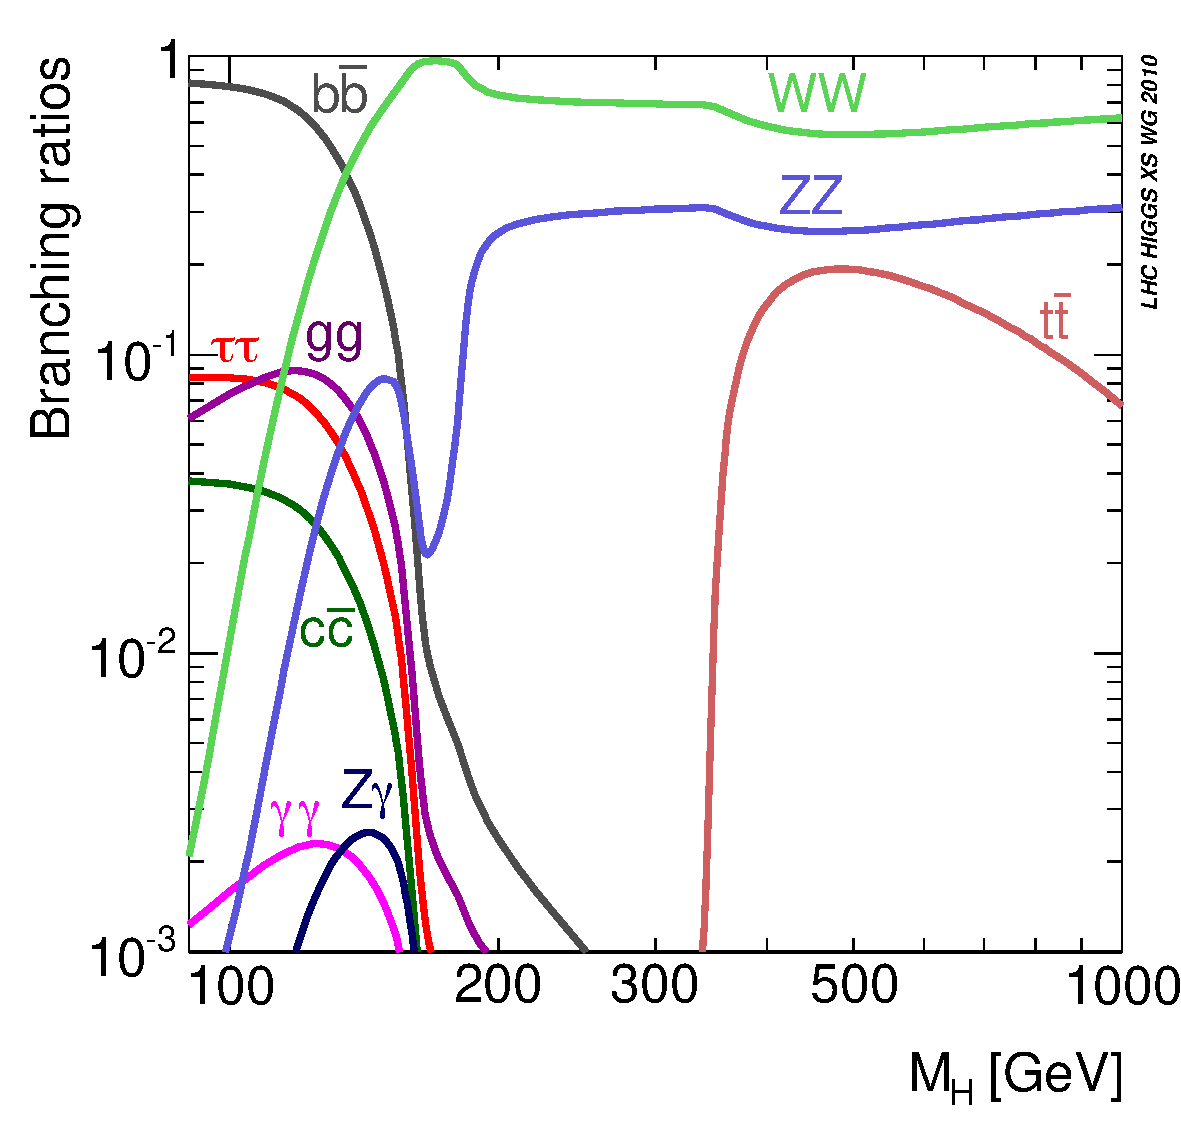
\includegraphics[width=0.47\textwidth,height=6cm]{imagens/higgs_branch_ratio.pdf}
        }%\hspace{0.1\textwidth}
        \subfigure[]{
            \label{fig:higgs_production}
            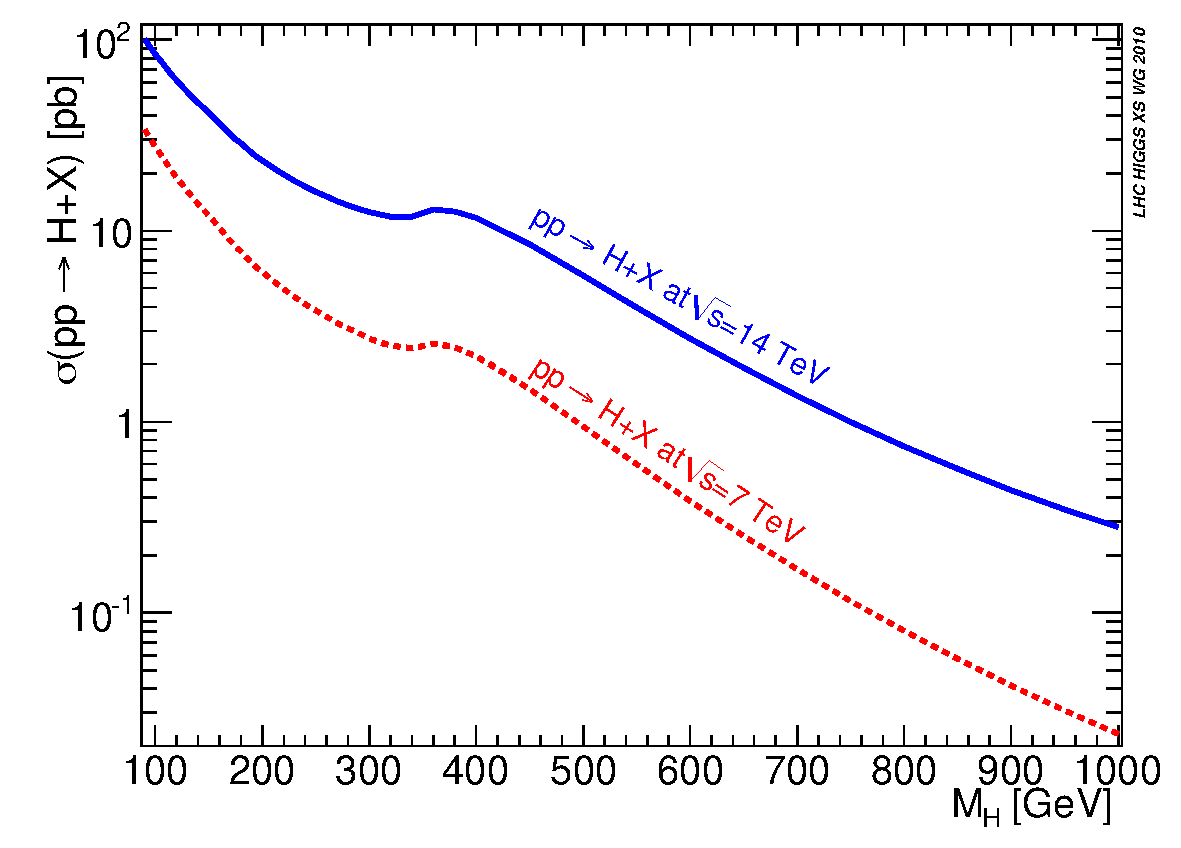
\includegraphics[width=0.47\textwidth,height=6cm]{imagens/higgs_production.pdf}
        }\\
        \subfigure[]{%
            \label{fig:higgs_sim_atlas}
            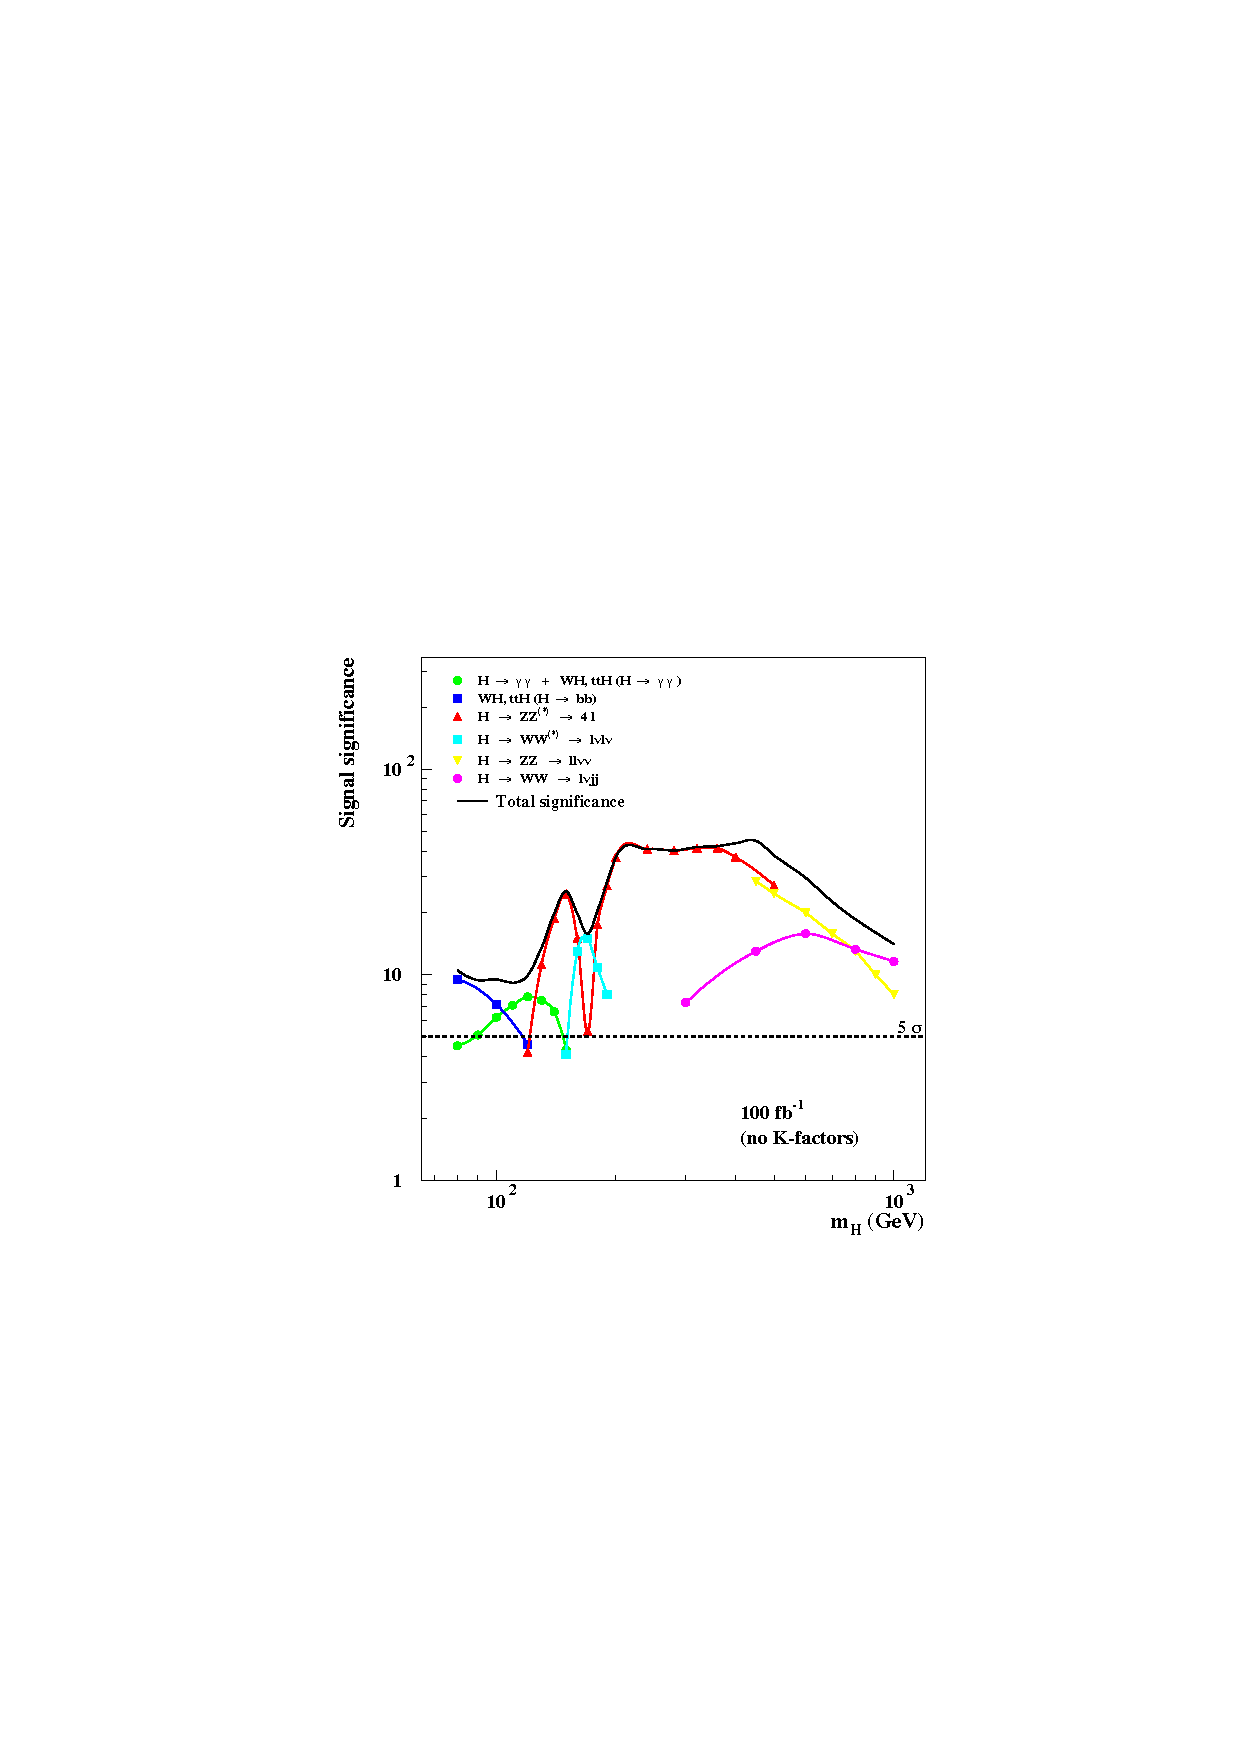
\includegraphics[width=.6\textwidth]{imagens/higgs_sim_atlas.pdf}
        }
    \end{center}
\caption[Simulação da significância dos canais de decaimento do bóssom
de Higgs explorados pelos ATLAS, as relações de seus canais e alcances em massa,
e a seção de choque do mesmo.]
{Os decaimentos do bóssom de Higgs do MP e suas relações de
seus canais e alcances em massa,~\ref{fig:higgs_branch_ratio}, e os seus valores de seção de choque para suas
respectivas massas,~\ref{fig:higgs_production}, ambos extraídas de \cite{lhc_higgs_group}. 
Em \ref{fig:higgs_sim_atlas} está uma simulação da significância dos possíveis canais de decaimento do
bóssom de Higgs, explorados pelo ATLAS, para uma luminosidade integrada de
$100fb^{-1}$, utilizando as eficiências esperadas para a detecção das
assinaturas dos estados finais e resoluções dos subdetectores, extraído de
\cite{ATLAS_TDR2}.}
\end{figure}

Observe que decaimentos do bóssom de Higgs mais frequentes não são,
necessariamente, os canais com melhor significância esperada. Aqueles canais em
que se tem mais facilidade de observar os decaimentos finais e poder associá-los
a produção de um bóssom de Higgs podem ter mais significância do que canais com
maior produção para uma dada massa. Isso reflete, por outro lado, na importância
dos algoritmos de reconstrução, obtendo melhor eficiência na reconstrução dos
estados finais facilitariam a encontrar o bóssom com menor quantidade de dados.
Os canais mais importantes nas regiões de massa intermediária, $\gls{mh}<2m_Z$,
onde se espera que os decaimentos reconstruam um pico de massa, são 
o canal de quatro léptons, $H\rightarrow ZZ^* \rightarrow 4l$, o canal de
produção direta em dois fótons, $H\rightarrow \gamma\gamma$, junto com os
canais de produção associada com o mesmo estados finais, . Para massas por volta
de 170 GeV/$c^2$, onde a produção de $ZZ^*$ é suprimida, o potencial da descoberta do
Higgs pode ser elevada pelo decaimento $H\rightarrow WW^*\rightarrow l\nu l\nu$,
nesse caso, o sinal deverá ser observado como um excesso de eventos. O canal de
quatro léptons com dois bóssoms Z reais é o dominante na região de
$\gls{mh}>2m_Z$, cobrindo uma vasta região de massa\footnote{Por isso chegou a
ser referenciado como canal banhado a ouro.}. Em massas mais elevadas, por volta de 600 GeV/$c^2$ até 1
TeV, outros canais como $H\rightarrow WW\rightarrow l\nu jj$, $H\rightarrow
WW\rightarrow ll\nu\nu$ são utilizados para a busca do bóssom de Higgs.

Posteriormente, outro canal foi adicionado, por outros estudos
\cite{atlas_tautau,atlas_tautau2}:

\begin{itemize} 
\item $H\rightarrow \tau \tau \rightarrow ll4\nu$ e $H\rightarrow \tau \tau
\rightarrow l\tau_{had}3\nu$ (110 a 150 GeV/$c^2$), onde $\tau_{had}$ seria o
decaimento do táon em píons especificados no início deste capítulo.
\end{itemize} 

Assim, a reconstrução de elétrons e múons fazem parte de grande
parte dos canais explorados para a vasta região de massa em que se espera
encontrar o bóssom de Higgs, inclusive um dos canais
mais importante por cobrir uma vasta região de massa. Se o Higgs existir com
uma massa mais baixa, os fótons serão necessários para poder encontrar o bóssom,
mostrando a importância do Canal \gls{eg}. 

\begin{figure}[t!]
    \label{fig:higgs_exclusion}
    \begin{center}
    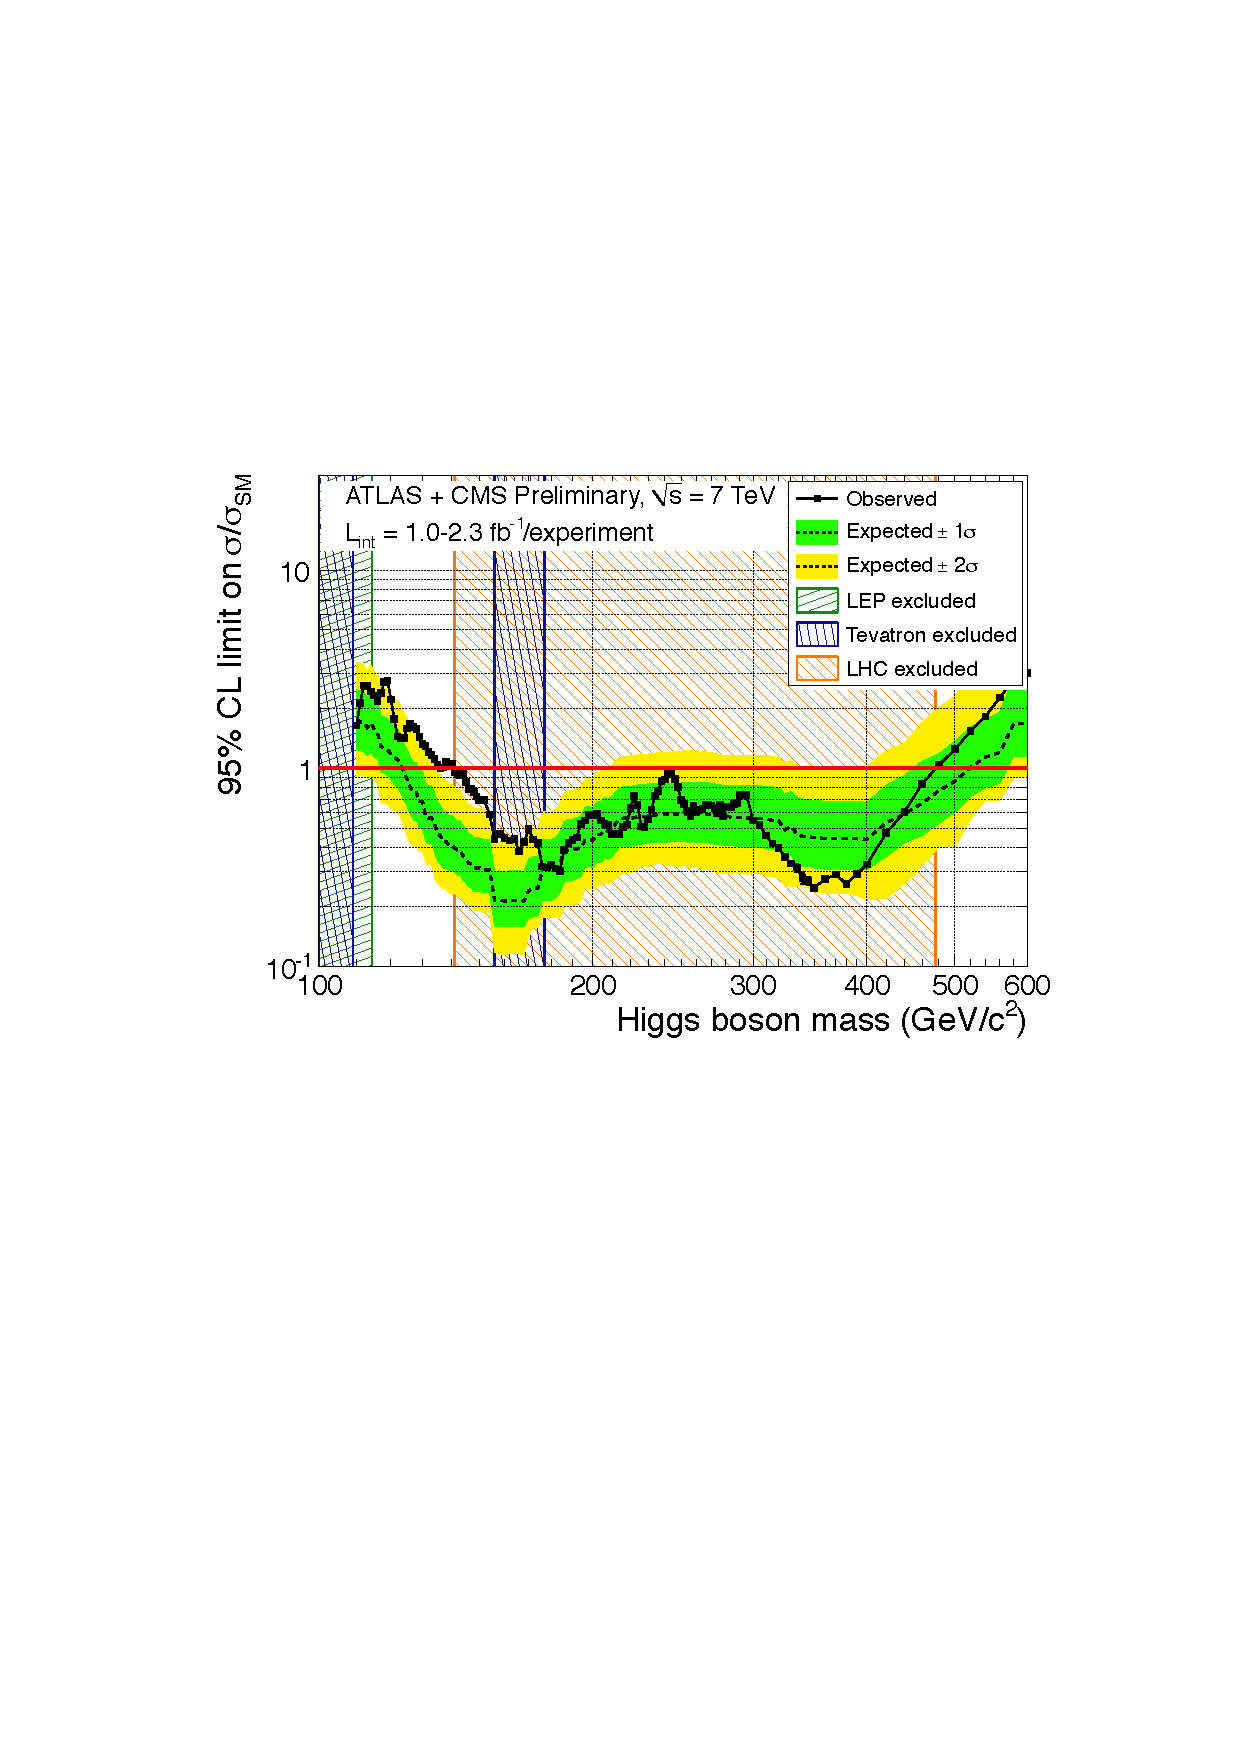
\includegraphics[width=0.8\textwidth]{imagens/exclusion_cms_atlas.pdf}
%
%        \subfigure[LEP, extraído de \cite{lep_higgs_2008}.]{%
%            \label{fig:lep_exclusion}
%            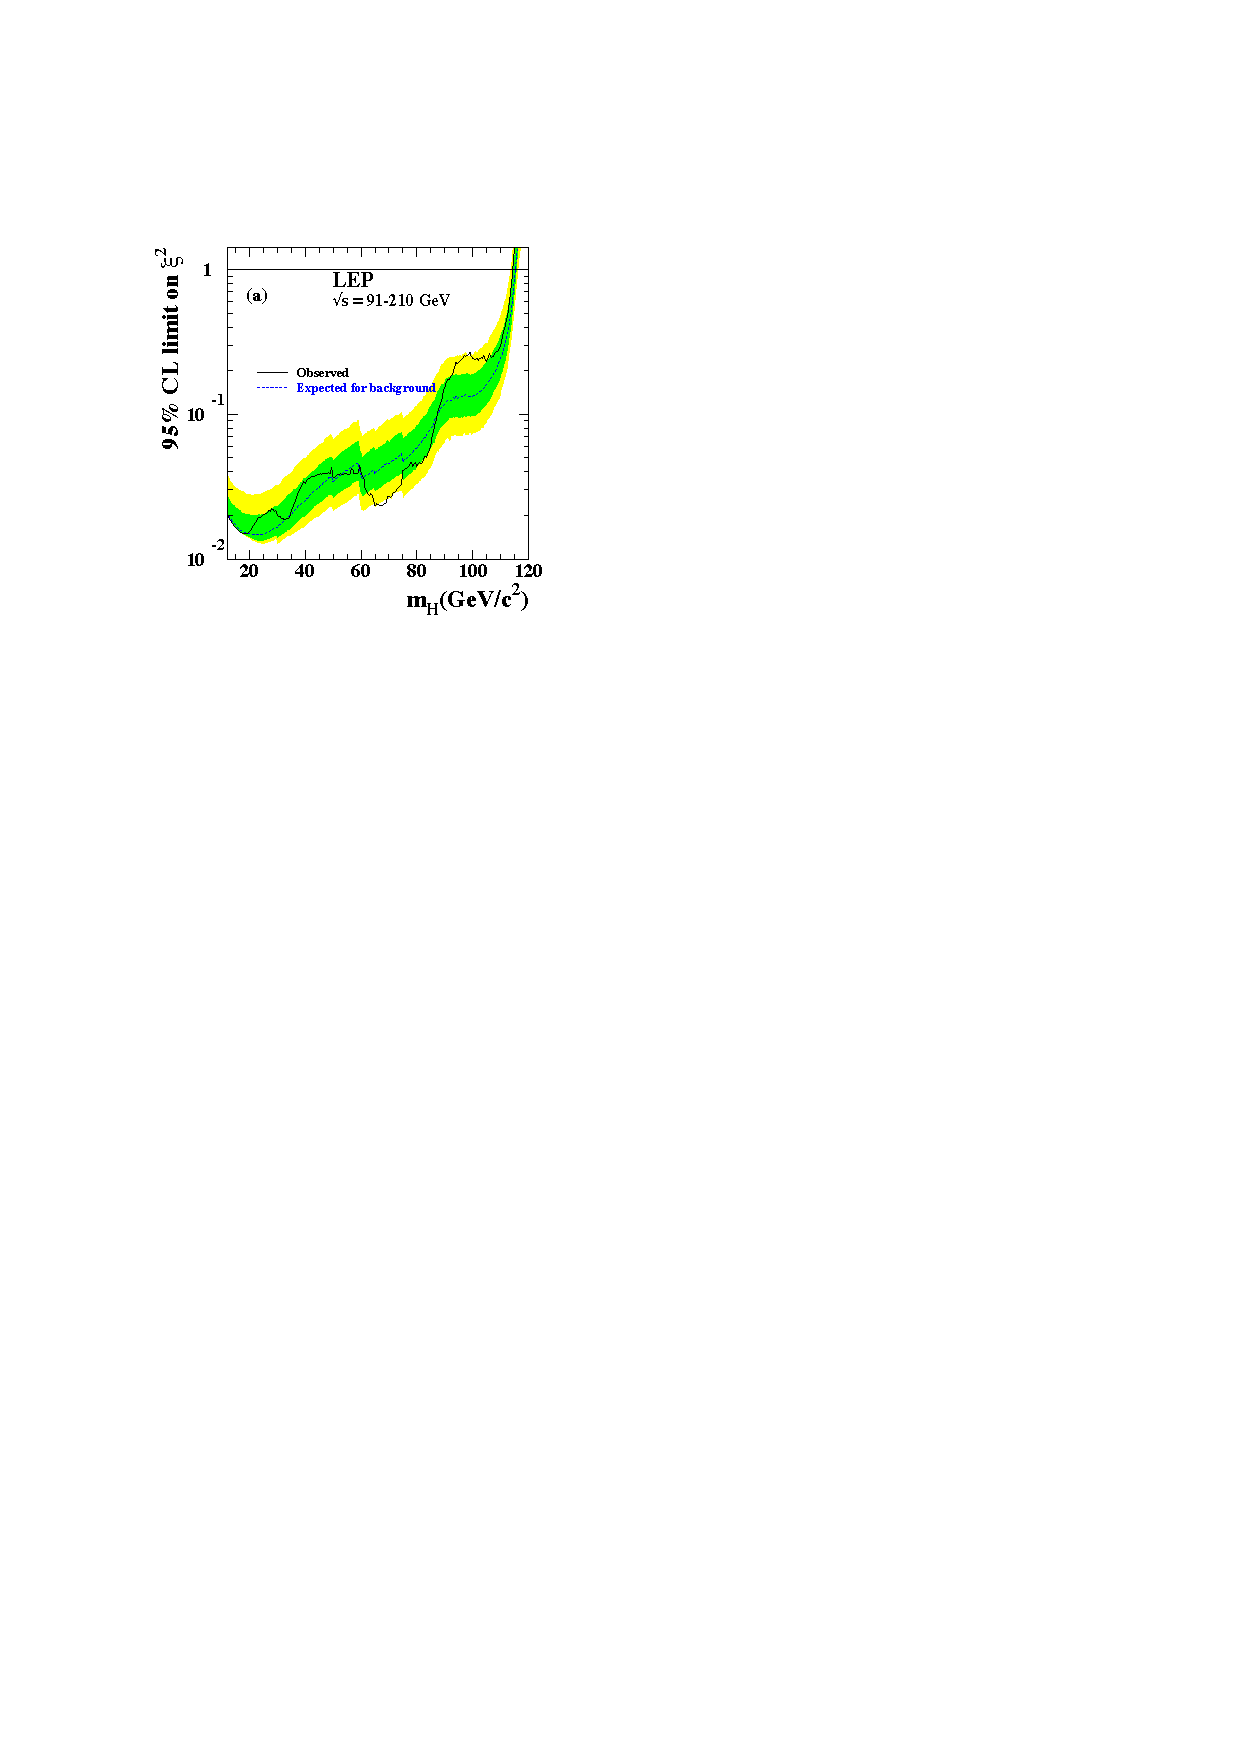
\includegraphics[width=0.47\textwidth]{imagens/lep_exclusion.pdf}
%        }%\hspace{0.1\textwidth}
%        \subfigure[Tevatron, extraído de \cite{tevatron_higgs}.]{%
%            \label{fig:tevatron_exclusion}
%            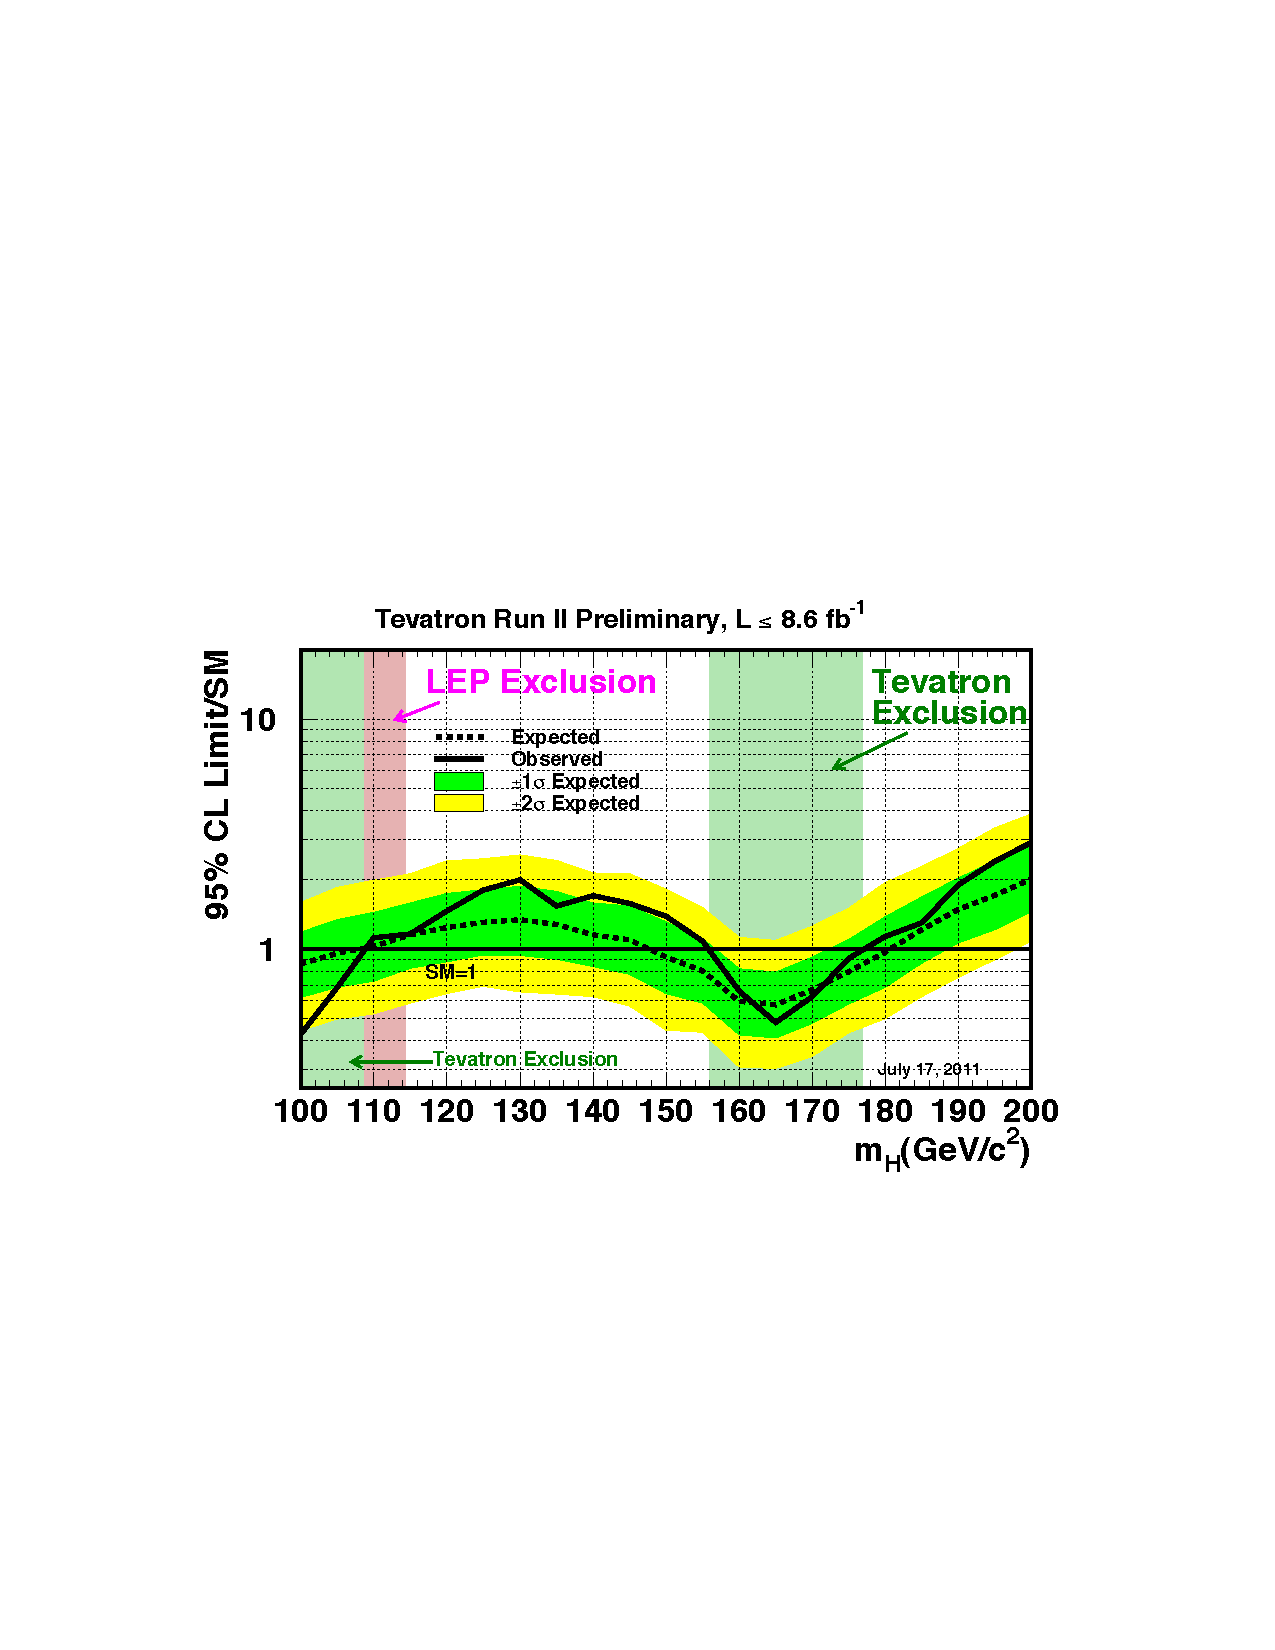
\includegraphics[width=0.47\textwidth]{imagens/tevatron_exclusion.pdf}
%        }\\%\hspace{0.1\textwidth}
%        \subfigure[ATLAS, extraído de \cite{atlas_higgs}.]{
%            \label{fig:atlas_exclusion}
%            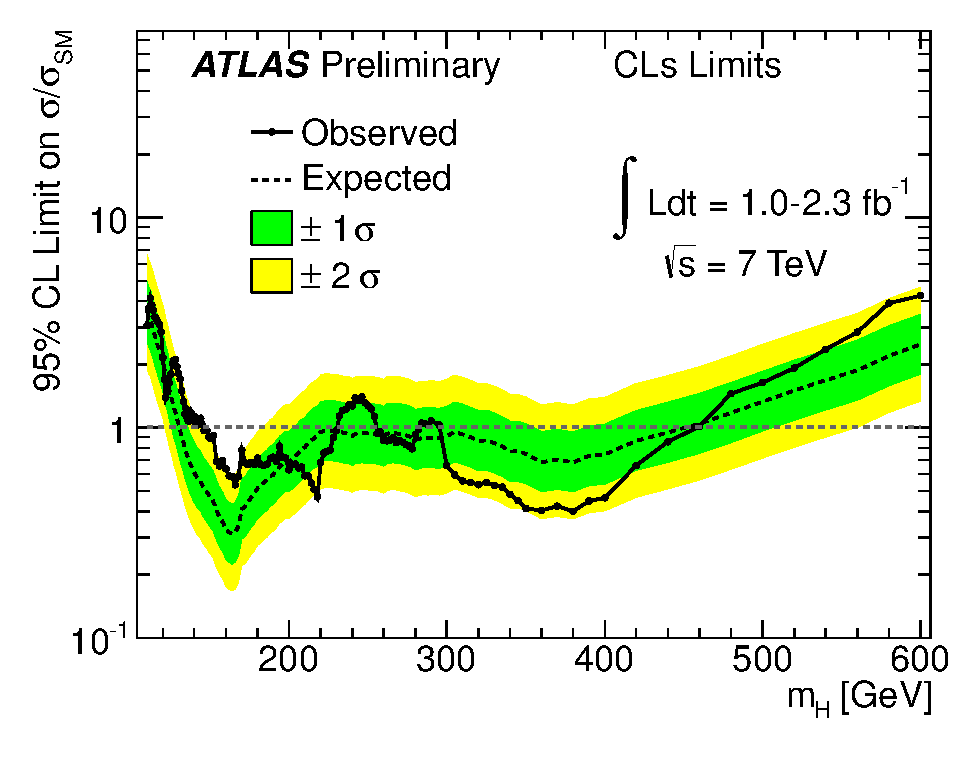
\includegraphics[width=0.47\textwidth]{imagens/atlas_exclusion.pdf}
%        }
%        \subfigure[CMS, extraído de \cite{cms_higgs}.]{%
%            \label{fig:cms_exclusion}
%            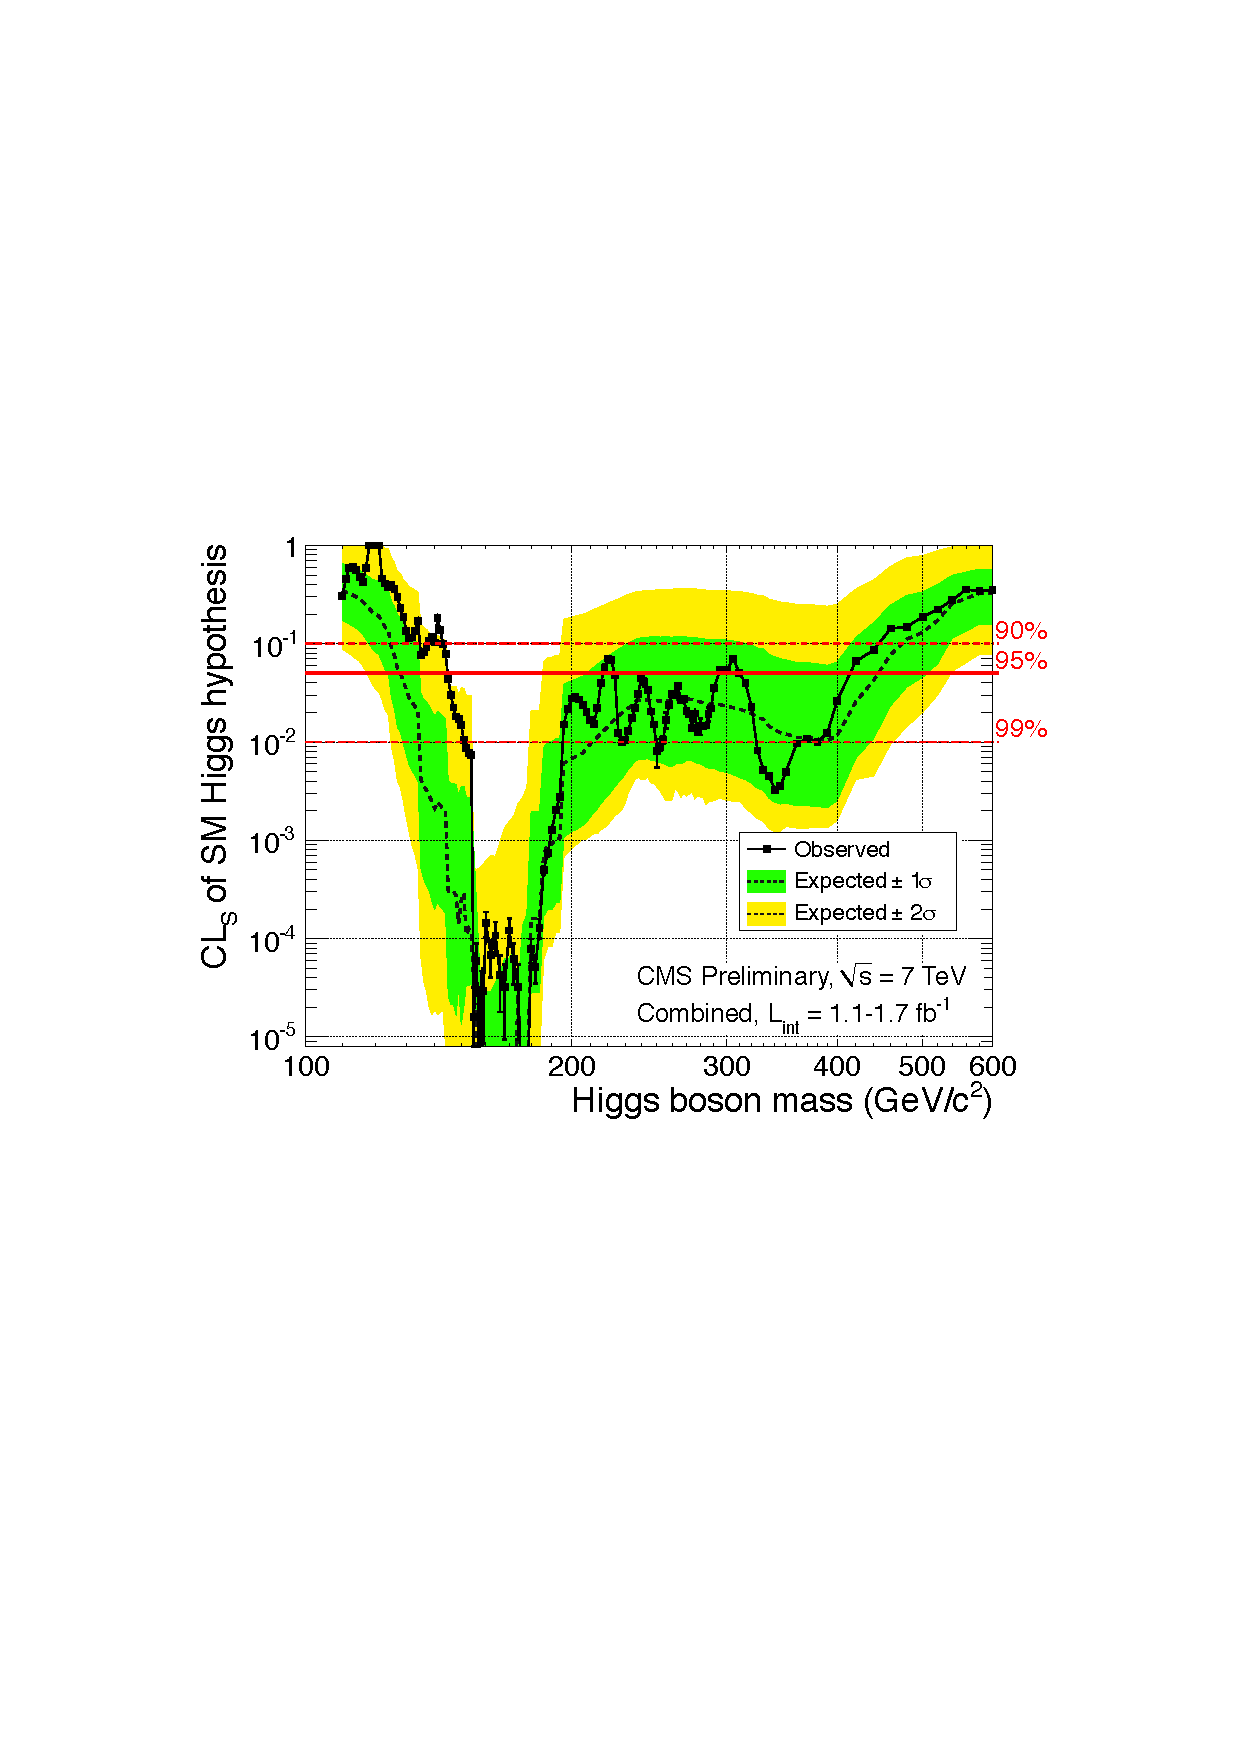
\includegraphics[width=0.47\textwidth]{imagens/cms_exclusion.pdf}
%        }
    \end{center}
\caption[Exclusões de massa do Higgs realizada pela combinação dos dados do
ATLAS e CMS. As exclusões de massa do Tevatron e LEP também estão indicadas.]{As exclusões de massa do bóssom de Higgs. Os valores de massa
observados, no caso para os resultados combinados do ATLAS e CMS, quando
abaixo da linha horizonal vermelha indicada são excluídos com um nível de
confiança de 95\%. A linha pontilhada indica o ruído de fundo esperado gerado
por física na ausência do bóssom de Higgs. As faixas verdes e amarelas indicam
um nível de certeza de 68\% e 95\% de certeza de que algo fora do comum está
ocorrendo. Caso a linha observada ultrapasse o limite superior da faixa amarela
em regiões acima da linha vermelha, então há 95\% de certeza de que há indícios
do bóssom de Higgs ou algum processo de física (talvez ruído físico) não bem
conhecido. Extraído de \cite{atlas_cms_higgs}.}
\end{figure}

Resultados mais recentes excluíram outras regiões de massa do bóssom de Higgs. Em 2008, 
o legado deixado pelo \gls{lep} elevou o limite inferior para 114 GeV/$c^2$
\cite{lep_higgs_2008}, enquanto o experimento Tevatron realizado pelo Fermilab, excluiu as
regiões de $156 < \gls{mh} < 177$ GeV/$c^2$, em Setembro de 2011
\cite{tevatron_higgs}. Também no final de Setembro, resultados preliminares do
\gls{atlas} excluíram o bóssom de Higgs para as regiões de 146-230 GeV/$c^2$, 256-282 GeV/$c^2$ 
e 296-459 GeV/$c^2$ \cite{atlas_higgs}. Um mês antes o \gls{cms} havia excluído o bóssom para
as regiões parecidas: de 145-216 GeV/$c^2$, 226-288 GeV/$c^2$ e 310-400 GeV/$c^2$
\cite{cms_higgs}. Em meados de Novembro o \gls{atlas} e \gls{cms} uniram seus
dados para excluir a região de 141-476 GeV/$c^2$ \cite{atlas_cms_higgs}. Esses
resultados estão indicados na Figura~\ref{fig:higgs_exclusion}, onde estão os
resultados mais recentes do \gls{lhc}, incluídas das regiões anteriormente
excluídas por outros experimentos.


\section{O Sistema de Filtragem (SF)}
\label{sec:sf}

\newacronym[type=Abrev]{asic}{ASIC}{Circuitos Integrados de Aplicação Específica}

O \gls{atlas}, para a luminosidade na qual tem operado: $\sim10^{33}cm^{-2}s^{-1}$,
gera cerca de 19 colisões inelásticas para cada cruzamento entre
feixes, que irão se cruzar numa frequência máxima de 40 MHz. O propósito do
\gls{sf} \cite{trigger_perf_2010,trigger_tdr} é de reduzir essa taxa a cerca
de 200 Hz para seu armazenamento e processamento a posteriori. Esse
limite, correspondendo uma média de $\sim$300 MB/s ($\sim$ 1,5 MB por evento de
cruzamento entre pacotes), é determinado pelos recursos
computacionais para armazenamento e processamento dos dados. É possível gravar
dados com taxas relativamente mais altas por períodos mais curtos, como foi
realizado durante 2010 quando a física foi beneficiada utilizando taxas de saída
de até $\sim$600 Hz. Nessa época, a luminosidade instantânea máxima atingida foi de
$\sim10^{32}cm^{-2}s^{-1}$, gerando cerca de $\sim$ 1,3 MB, e o \gls{lhc} não 
operava de forma continua -- o que é comum para um acelerador novo -- permitindo 
elevar a taxa de armazenamento.

\subsection{A estrutura do Sistema de Filtragem}
\label{ssec:estru_sf}
\newacronym[type=Abrev]{rob}{ROB}{\emph{Buffer} de Leitura}
\newacronym[type=Abrev]{ros}{ROS}{Sistemas de Leitura}

O \gls{sf}, Figura~\ref{fig:sf_esboco}, é dividido em três níveis sequenciais,
sendo descrito aqui resumidamente uma vez que já foi explicada em maiores detalhes em
trabalhos anteriores como \cite{tese_eduardo,tese_torres}, também podendo ser encontrada 
em detalhes nas referências \cite{trigger_tdr,l1_trigger_tdr,l2_ef_daq_dcs_tdr,trigger_perfomance}.

Os sinais do detector são armazenados em memórias \emph{pipeline}, com pendência
à decisão do \acrshort{l1}. Para obter uma latência de menos de 2,5 $\mu$s, 
o \gls{l1} é implementado em rápida eletrônica constituída de \gls{fpga} e
\gls{asic}, de forma a reduzir a taxa para uma valor máximo de 75 kHz. Para
aumentar a velocidade, esse nível utiliza apenas a informação dos subsistemas de
calorimetria e câmaras de múons com granularidade reduzida. Além do
primeiro passo de seleção, o \gls{l1} identifica as \glspl{roi} do detector a
serem investigadas pelo \acrshort{hlt}. 

\begin{figure}[ht!]
\label{fig:sf_esboco}
\centering
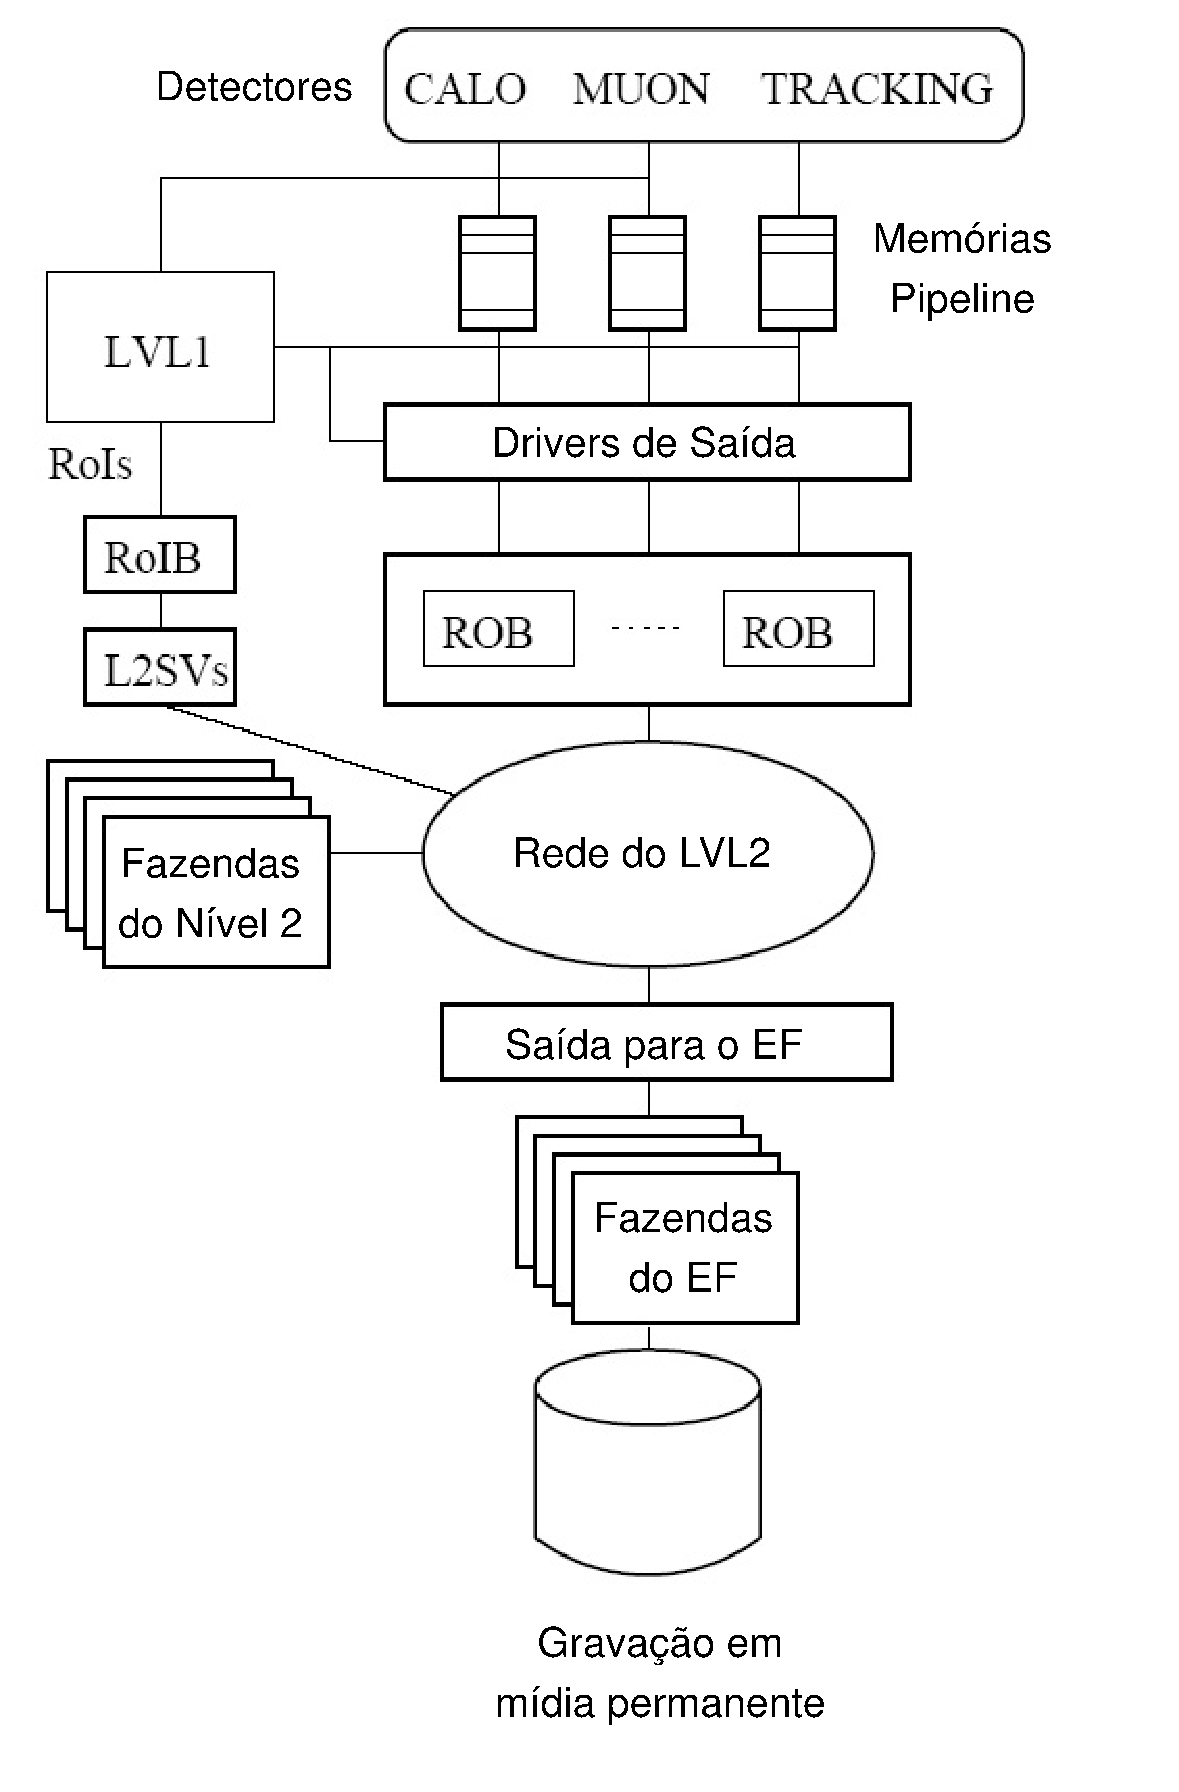
\includegraphics[width=0.6\textwidth]{imagens/sf_resumo.pdf}
\caption[Esboço do Sistema de Filtragem.]{Esboço do Sistema de Filtragem. Extraído de \cite{tese_eduardo}.}
\end{figure}

O \gls{hlt} se consiste de fazendas de
processadores comerciais conectados a rede dedicadas (\emph{Ethernet} de \emph{Gigabit} 
e 10 \emph{Gigabit}).  O \gls{sf} foi projetado para conter cerca de 500 nós para o
\acrshort{l2} e 1800 nós para o \acrshort{ef}\footnote{Em 2010, a fazenda de processamento 
se consistia de 800 nós configuráveis como tanto \acrshort{l2} ou \acrshort{ef}, este 
contendo mais 300 nós dedicados.}. Quando um evento é aceito pelo
\gls{l1}, os dados na memória de cada um dos detectores são então transferidos
para \gls{rob} específicos para cada um dos subdetectores, que armazenam o
evento em fragmentos pendendo à decisão do \gls{l2}. Um ou mais \glspl{rob} são
agrupados para formar os \gls{ros} que são conectados a rede do \gls{hlt}. O
seleção do \gls{l2} é baseada em algoritmos personalizados e rápidos que
processam os dados dos eventos de forma parcial nas regiões especificadas pelas
\glspl{roi} identificadas pelo \gls{l1}. Os processadores do \gls{l2} solicitam os
dados dos \gls{ros} correspondentes aos elementos do subdetector dentro de cada
\gls{roi}, reduzindo a quantidade de dados a serem transferidas e processadas no
mesmo a cerca de 2-6\% do volume total dos dados. O \gls{l2} reduz a taxa de
dados para cerca de $\sim$3 kHz com uma média de processamento de $\sim$40
ms/evento. Qualquer evento com tempo excedendo a 5 s nesse nível é perdido a
rotulado como evento excedente ao tempo limite.   

O \gls{ef} reúne todos os fragmentos dos eventos aceitos pelo \gls{l2} das
\glspl{rob}, tendo assim acesso a toda sua informação. O \gls{ef} é, em grande
maioria, baseado nos algoritmos do \acrlong{sr} rodando em interfaces
personalizadas para o ambiente do \gls{sf}. Esse nível é projetado para reduzir
os dados para $\sim$200 Hz com uma média de processamento de $\sim$4 s/evento.
Qualquer evento com um tempo excedente a 180 s também é rotulado e perdido como
no \gls{l2}. 

Os eventos de dados selecionados pelo \gls{sf} são escritos nos fluxos de dados
inclusivos, baseados no canal de filtragem. Existem quatro canais de dados
primários, cada um com uma banda pré-determinada (taxa em Hz utilizada na
luminosidade de $10^{32}cm^{-2}s^{1}$): Egamma (50),
Muons (50), JetTauEtMiss (65), Minbias (10), adicionados de diversos canais
de calibração (13). Cerca de 10\% dos eventos são escritos 
para um canal expresso aonde a reconstrução pronta dos eventos é realizada, como foi dito na
Subseção~\ref{ssec:lcg}. Ainda, além da gravação de eventos completos em um
canal, é possível escrever informação parcial de um ou mais subdetectores em um
canal, o que é normalmente realizado para a calibração do detector nos canais
destinados a esse propósito.


\subsection{Topologia dos algoritmos e sua configuração}
\label{ssec:alg_topo}

\newacronym[type=Abrev,\glslongpluralkey={Algoritmos de Extração de
Características}]{fex}{FEX}{Algoritmo de Extração de Característica}
\newacronym[type=Abrev,\glslongpluralkey={Algoritmos de Hipótese}]
{hypo}{HYPO}{Algoritmo de Hipótese}

A configuração do \gls{sf} é realizada por um \emph{menu}, que define as
\emph{cadeias} de filtragem que especificam uma sequência de passos de reconstrução e
seleção para as especificas assinaturas de filtragens requeridas pela filtragem.
A cadeia de filtragem de elétrons é ilustrada na Figura~\ref{fig:electron_chain}.
Cada \emph{cadeia} é composta pelo \gls{fex} que criam objetos,
como os aglomerados de células e variáveis que permitam obter uma informação
sobre a descrição do evento, e pelo \gls{hypo} que fazem a discriminação através dos
critérios de seleção nos objetos gerados, como por exemplo a exigência de um
$\gls{pt} > 20$ GeV. As extrações de características realizadas por uma
\emph{cadeia} podem ser reutilizadas por outro cadeia, reduzindo tanto o acesso
a dados como o tempo de processamento do \gls{sf}.

\begin{figure}[ht!]
\label{fig:electron_chain}
\centering
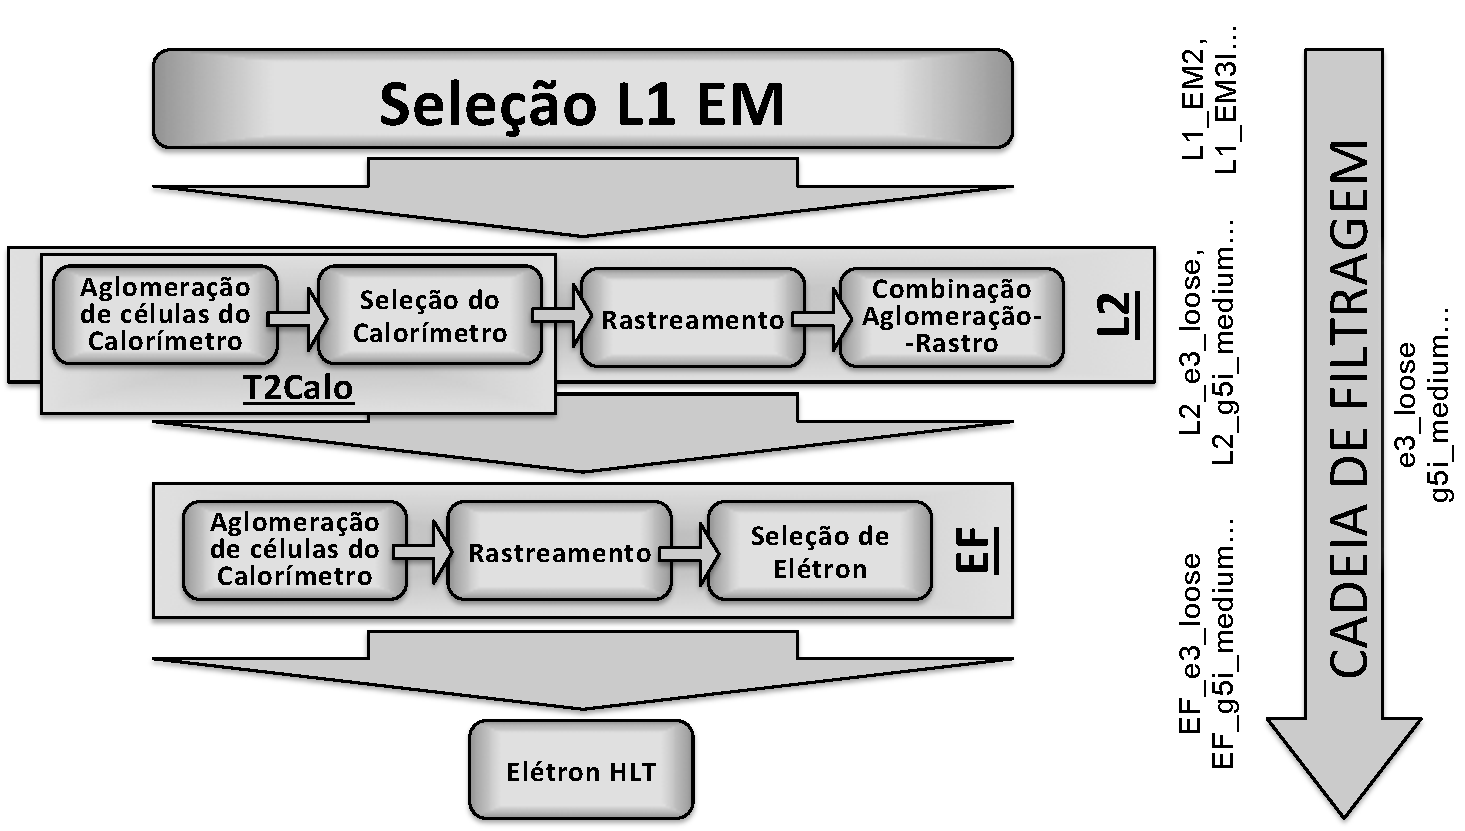
\includegraphics[width=0.9\textwidth]{imagens/cadeia_eletron.pdf}
\caption[A \emph{cadeia} de filtragem de elétrons.]{A \emph{cadeia} de filtragem
de elétrons. A direita de cada nível de filtragem estão colocados exemplos de
nomes de filtros de elétrons e fótons, e o nome de sua respectiva cadeia a
direita da seta indicando a evolução da \emph{cadeia}. Adaptado de \cite{trigger_perf_2010}.}
\end{figure}

Aproximadamente 500 filtros são definidos nos \emph{menus} atuais, sendo
composto por um número de diferentes classes de filtros:

\begin{itemize}
\item \textbf{Objetos de filtro único}: usado para determinar estados com pelo
menos um objeto característico. Por exemplo, um filtro para elétron único com um
limiar nominal superior a 3 GeV seria referido como $e3$;
\item \textbf{Objetos de filtro múltiplos}: usado para determinar estados finais
com dois ou mais objetos do mesmo tipo. Por exemplo, elétrons duplos decaindo da
partícula $\text{J}/\Psi$. Esses filtros são indicados dependendo de sua
multiplicidade, por exemplo: $2e3$;
\item \textbf{Objetos de filtro combinados}: usados por estados finais de dois
ou mais objetos característicos de tipos diferentes. Por exemplo, um múon de 13
GeV adicionado de 20 GeV de \gls{Etmiss} para selecionar decaimentos
$W\rightarrow \mu\nu$, que seriam denotados de $mu13\_xe20$;
\item \textbf{Filtros Topológicos}: usados para estados finais selecionados de
duas ou mais \glspl{roi}, como no caso do decaimento da partícula
$\text{J}/\Psi$, que combina os traços das duas \glspl{roi} provenientes dos
elétrons.
\end{itemize}

Quando se referindo a um nível em particular, o nível (\gls{l1}, \gls{l2},
\gls{ef}) aparece como um prefixo, como por exemplo L1\_EM3 (aqui elétrons e
fótons não são diferenciados, então se utiliza o prefixo EM em ambos os casos)
para denotar um filtro de elétrons e fótons com um limiar nominal superior a 3
GeV para o \gls{l1} e L2\_e3 no caso de elétrons para um filtro com o mesmo
limiar mas para elétrons apenas no \gls{l2}. Um nome sem o prefixo de nível
refere-se a toda a \emph{cadeia}.

O controle das taxas de filtragem podem ser realizadas mudando os limiares ou
aplicando outros valores de seleção. A seletividade de um grupo de cortes
aplicados para um certo objeto de filtragem é representado pelos termos
\emph{Loose} (relaxado), \emph{Medium} (mediano), \emph{Tight} (apertado). Esses
critérios de seleção são colocados como sufixos ao nome do filtro, por exemplo,
e10\_medium. Requerimentos adicionais como isolamento, podem ser adicionados
para reduzir as taxas dos filtros. O isolamento mede a quantidade de energia, ou
o número de partículas próximos a uma assinatura, se esse valor estiver acima de
um limiar, então a partícula não está isolada. Nesse caso se adiciona a letra
'i' ao nome do filtro, como por exemplo L1\_EM20I ou e20i\_tight.

Fatores de \emph{pré-escala} podem ser adicionados a cada filtro da 
\emph{cadeia} do \gls{hlt}, de tal forma que apenas 1 em cada N eventos passando
o filtro causam que o evento seja aceito por aquele nível. A \emph{pré-escala}
controla a taxa e composição dos canais expressos. Uma série de
\emph{pré-escalas} são utilizadas baseadas em diversas regras que levam em
consideração a prioridade dos filtros em relação com as seguintes categorias:

\begin{itemize}
\item \textbf{Filtros Primários}: filtros principais de física, que não deveriam
ser \emph{pré-escalados};
\item \textbf{Filtros de Suporte}: filtros importantes de suporte a filtros
primários, como filtros que permitam estudar a eficiência utilizando 
seletividades mais baixas e limiar mais baixo de \gls{Et} \emph{pré-escalados}
para permitir sua gravação em disco, uma vez que a quantidade de dados que
passam esse filtro será maior;
\item \textbf{Filtros de Monitoração e Calibração}: permitindo a coleta de dados
para garantir a operação correta do \gls{sf} e dos subdetectores do \gls{atlas},
incluindo a calibração dos mesmos. 
\end{itemize}

\newacronym[type=Abrev]{lb}{LB}{Bloco de Luminosidade} 

Esses fatores de \emph{pré-escala} devem ser modificados conforme a queda da
luminosidade durante um preenchimento do \gls{lhc} de forma a garantir a
maximização das taxas utilizadas pelos filtros, enquanto garantindo uma taxa
constante para a monitoração e calibração. Assim, as mesmas podem ser alteradas
em quaisquer momentos de uma temporada, no início de um novo \gls{lb}. Um
\gls{lb} é a unidade fundamental para a medição da luminosidade, cerca de 120 s
em 2010, na qual se considera que a mesma permaneceu constante com o valor
medido.

Flexibilidade adicional é oferecida ao definir \emph{grupos de pacotes}, separando os
filtros para colisões com pacotes emparelhados (compõe as colisões de física
regulares, contendo pacotes de feixes opostos que se encontram no ponto de
colisão simultaneamente), pacotes vazios para estudo de pedestal criado por ruído 
no detector e raios cósmicos, ou até mesmo configurações mais inusitadas, como 
exigindo pacotes desparelhados separados por no mínimo 75 ns de quaisquer outro 
pacote no feixe oposto.



\subsection[Algoritmos Padrões da \emph{Cadeia} de Filtragem de eGamma]{Algoritmos Padrões da \emph{Cadeia} de Filtragem de $e/\gamma$}
\label{ssec:cadeia_egamma}

\newacronym[type=Abrev,\glslongpluralkey={Torres de Filtragem}]
{tt}{TT}{Torre de Filtragem}

O sistema de calorimetria do \gls{atlas} cobre uma região de $|\gls{eta}| <
4,9$, enquanto o \gls{id} fornece reconstrução precisa de traços dentro de
$|\gls{eta}| < 2,5$. Os chuveiros \gls{em} são reconstruídos com melhor
performance para essa última região, a região de precisão do \gls{atlas}, 
contendo calorímetros com maior granularidade como descrito na
Subseção~\ref{ssec:calorimetria}. Assim, os filtros de elétrons e fótons
\cite{expected_perf_2011,perf_2011} do \gls{sf} atuam somente para essa região.
A cadeia de elétrons no \gls{sf} está esboçada na Figura~\ref{fig:electron_chain}, entretanto
a cadeia de fótons pode ser facilmente extrapolada ao se remover os algoritmos
referentes ao \gls{id}.

No \gls{l1}, os aglomerados de informação\footnote{No caso, um conjunto de
células identificados como \emph{clusters} na literatura em inglês.} \gls{eg} do calorímetro são retirados
utilizando granularidade reduzida, as chamadas \glspl{tt}, que cobrem uma região
de aproximadamente $\Delta\eta\times\Delta\phi\approx0,1\times0,1$, 
a Figura~\ref{fig:cal_lar_camadas} contem um esboço da \gls{tt} para o
\gls{emb}. A vantagem de se utilizar \glspl{tt} se deve ao
fato de reduzir a quantidade de fluxo de informação, reduzindo o custo e
complexidade do sistema, e, ao mesmo tempo, conter o chuveiro \gls{em} inteiramente 
em cerca de uma ou duas dessas torres, podendo
assim identificar a região em que foi formado o chuveiro não prejudicando a sua
eficiência. Para cada \gls{tt}, as células do \gls{ecal} e \gls{hcal} são somadas, com a
exceção da quarta camada do \gls{hec} e dos cintiladores.
Um algoritmo de janela deslizante formada por uma dimensão de $4\times4$
\gls{tt}, ilustrada na Figura~\ref{fig:sliding_window_l1}, 
busca pela região com a melhor deposição de energia do chuveiro por
todo o calorímetro com um passo de uma \gls{tt}.
O \gls{l1} seleciona o evento como um candidato a \gls{eg} 
quando os seguintes critérios forem satisfeitos:

\begin{figure}[ht!]
\label{fig:l1_alg}
\centering
        \subfigure[A janela deslizante, seu núcleo e as regiões de isolamento.]{
            \label{fig:sliding_window_l1}
            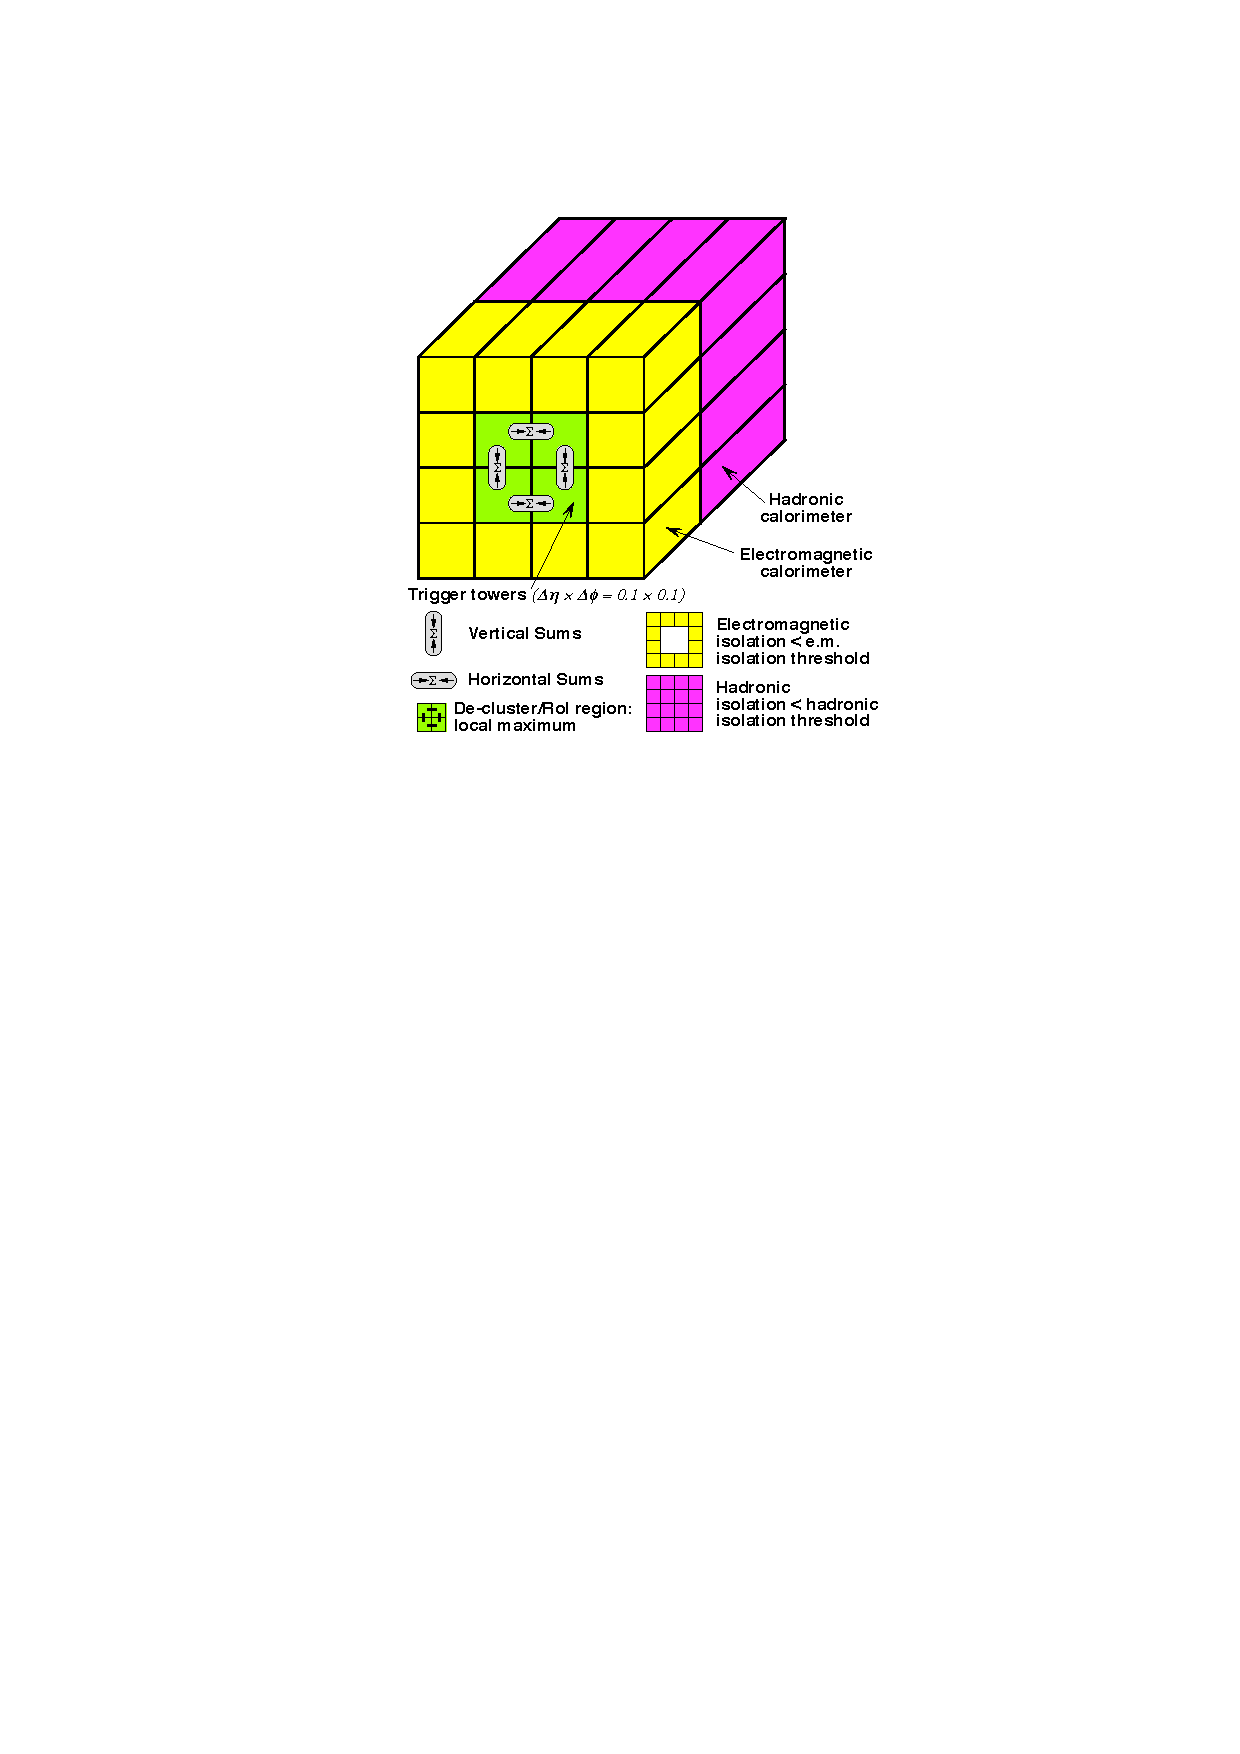
\includegraphics[width=0.6\textwidth]{imagens/sliding_window_l1.pdf}
        }\hspace{0.01\textwidth}
        \subfigure[Requerimento para o núcleo ser máximo local.]{%
            \label{fig:local_et}
            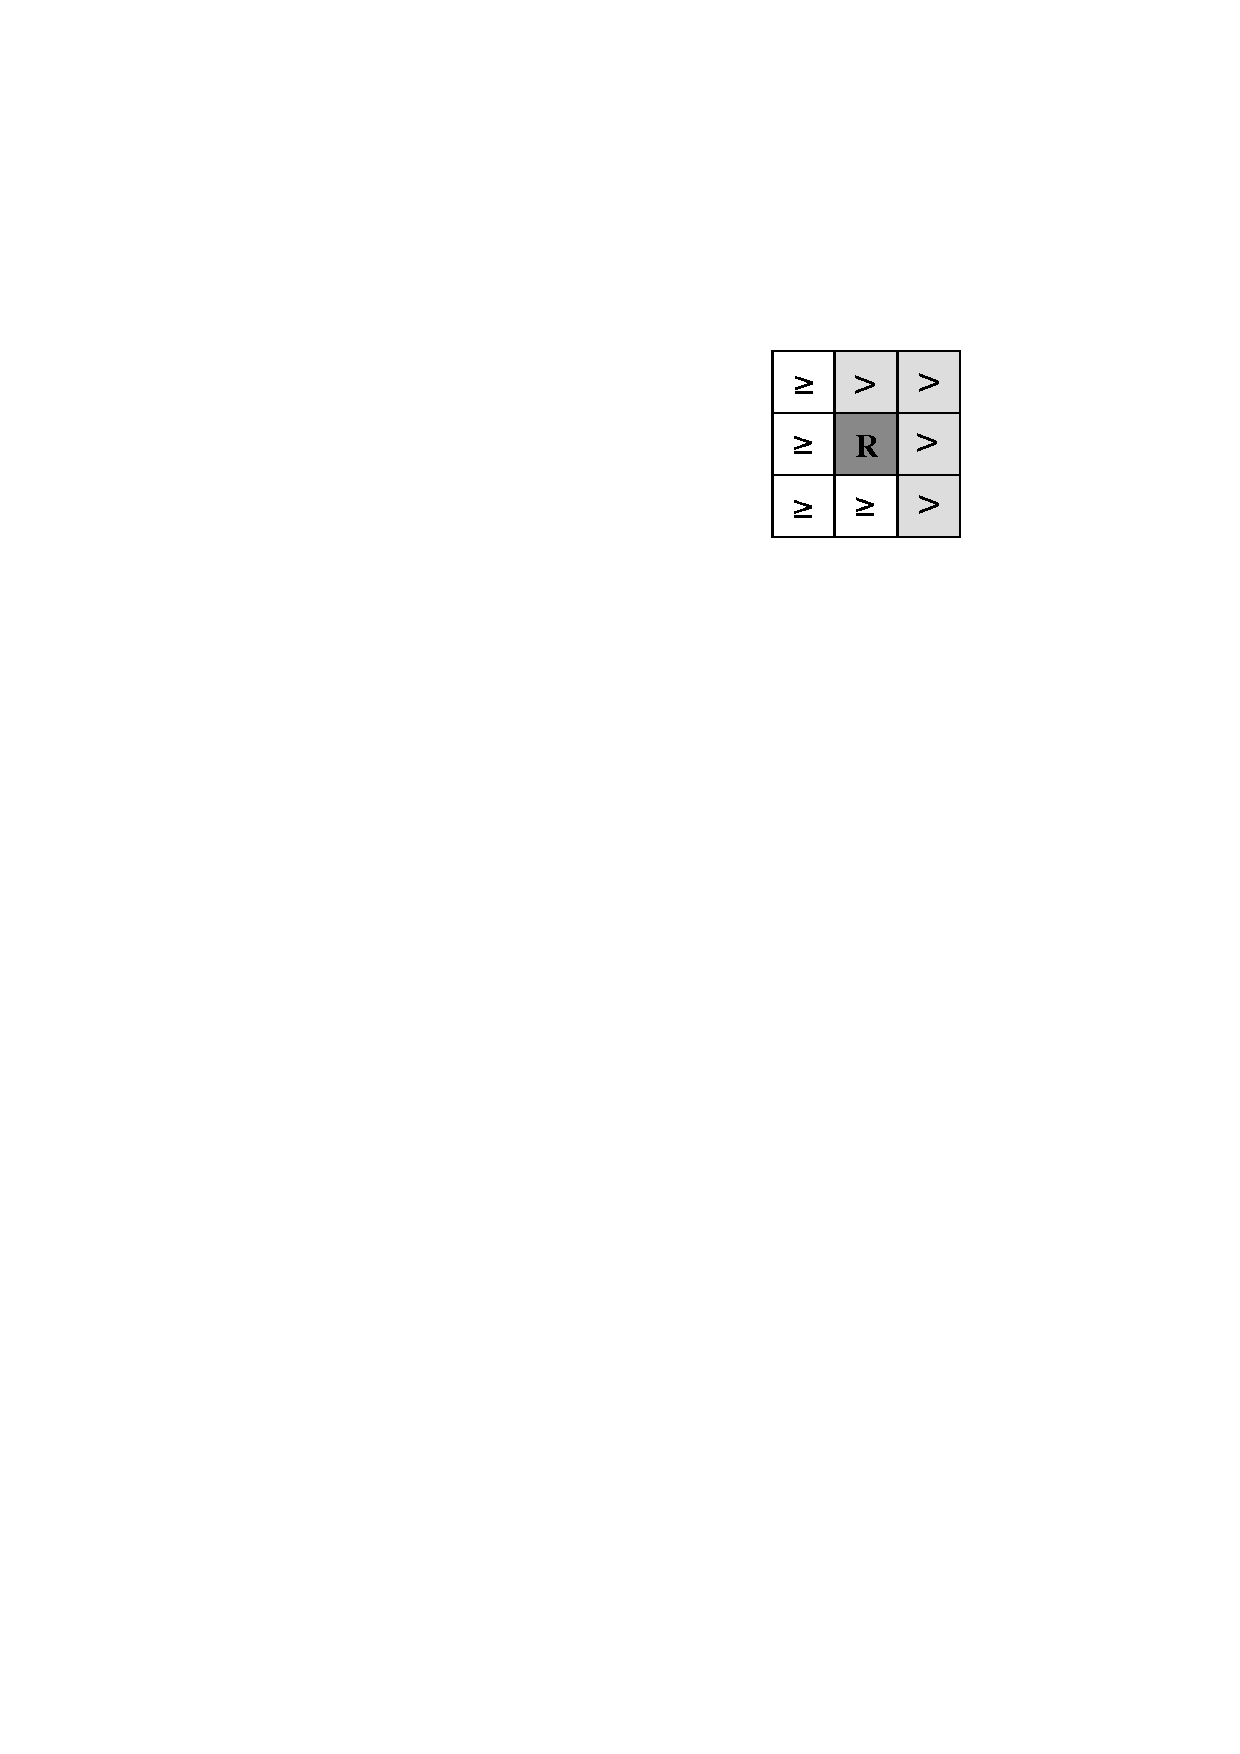
\includegraphics[width=0.3\textwidth]{imagens/roi_local_max.pdf}
        }
\caption[O Primeiro Nível de Filtragem para a Cadeia de Elétrons e Fótons.]
{O Primeiro Nível de Filtragem para a Cadeia de Elétrons e Fótons. Extraído de
\cite{l1_trigger_tdr}.}
\end{figure}

\begin{itemize}
\item A região deve ser um máximo local. Essa condição é importante para se
evitar multiplicidade de \glspl{roi} a serem analisadas pelo \gls{l2}.
Assim, a energia contida no núcleo deve ser
maior, ou ao menos igual, como na lógica da Figura~\ref{fig:local_et}, 
que em todos as outras regiões de $2\times2$ que podem ser formados na
janela;
\item O aglomerado formado pela dupla de torre mais energética na região
(indicados na Figura~\ref{fig:sliding_window_l1} como somas verticais ou horizontais) deve ultrapassar o limiar
\gls{em} exigido pelo filtro do \gls{l1}. A posição de \gls{eta} e \gls{phi} desse aglomerado é passado
para o \gls{l2}, junto com outros \emph{bits} indicando os critérios que foram
satisfeitos, que formarão a palavra informada para o \gls{l2} para a qual será
utilizada para a formação da \gls{roi};
\item Se isolamento for exigido: 
\begin{itemize}
\item A \gls{Et} total da região \gls{em} de
isolamento não deve ultrapassar o limiar de isolamento \gls{em};
\item A \gls{Et} total da região \gls{had} de isolamento não deve ultrapassar o
limiar de isolamento \gls{had}.
\end{itemize}
\end{itemize}


O \gls{l2}, alimentado pela posição dos
aglomerados de torres do \gls{l1}, realiza uma rápida reconstrução do
calorímetro, e no caso de elétrons, uma rápida reconstrução dos traços no \gls{id}. A
reconstrução do calorímetro trabalha de maneira semelhante aos algoritmos do
\gls{sr}, entretanto apenas a região da janela de $\Delta\eta\times\Delta\phi =
0,4 \times 0,4$, região chamada de \gls{roi}, em torno da posição alimentada pelo \gls{l1} 
é utilizada, o que reduz o tráfico de dados e aumenta a velocidade de processamento no \gls{l2}.
Algumas diferenças entre o algoritmo do \gls{l2} e o \gls{sr} se dão as
limitações no tempo de latência. O algoritmo de reconstrução do aglomerado de
células do calorímetro no \gls{l2} começa utilizando a célula mais energética da
\gls{e2} dentro da região central de $0,2 \times 0,2$, enquanto o
algoritmo de análise a posteriori utiliza uma janela deslizante para encontrar
sua semente.

No \gls{l2}, o tamanho do aglomerado é fixado para $3
\times 7$ células em $\gls{eta} \times \gls{phi}$ para o barril ($|\gls{eta}|<1,5$) e 
$5 \times 5$ na tampa ($1,5<|\gls{eta}|<2,5$). O algoritmo a posteriori possui
tamanhos diferentes dependendo do tipo de partícula e se a incidência foi no
barril ou na tampa. No caso de incidência no barril, elétrons são reconstruídos
através de aglomerados com $3\times7$ torres; fótons $3\times5$, 
e fótons convertidos em elétrons, $3\times7$. Na tampa todos os aglomerados 
são de $5\times5$.

As energias das células podem ser corrigidas na análise a posteriori, para
problemas transientes no \emph{hardware}, como falhas de energia, etc., o que não
pode ser realizado em tempo real, o que se aplica para tanto o \gls{l2} e
\gls{ef}. Para a reconstrução de traços no \gls{l2}, um rápido reconhecimento de
padrões é utilizado ao se determinar primeiro a posição z de interação ao longo
do eixo do feixe e então realizando a combinação de pontos do traço apenas para o grupo
de pontos que apontam para a posição determinada. O traço com a menor distância
$\Delta R$, definida por \ref{eq:dist_clust_traco}, será atribuído ao
aglomerado e seus parâmetros utilizados pelo \gls{l2} para a discriminação.

\begin{equation}\label{eq:dist_clust_traco}
\Delta R = \sqrt{\Delta^2\eta+\Delta^2\phi}
\end{equation}

Como no \gls{sr}, a reconstrução do aglomerado no \gls{ef} é realizado
utilizando um algoritmo de janela deslizante que será
explicado em \ref{ssec:egamma}. Basicamente, após encontrada
a semente através do máximo local, um aglomerado é construído iniciando da \gls{e2},
com o mesmo tamanho que aqueles descritos para o algoritmo a posteriori. O
centro de distribuição de energia em \gls{eta} e \gls{phi} é calculado
utilizando o aglomerado construído na \gls{e2}, e então o valor dessa
posição é propagado de forma a incluir as camadas faltantes. O algoritmo
de reconstrução de traços é feito como no algoritmo a posteriori, com uma
combinação dos traços começando dos pontos dos Detectores de Silicone e
\gls{trt}.

Os algoritmos de seleção são aplicados na reconstrução do
\gls{l2} e no \gls{ef} com o objetivo de identificar bons candidatos a \gls{eg}
e rejeitar falsos alarmes provenientes de jatos. As seleções são baseadas no
formato do chuveiro nas aglomerações, tentando identificar as diferenças já
citadas entre os chuveiros \gls{em} e \gls{had} no
Subtópico~\ref{par:cal_part_id}, como: a largura dos chuveiros, onde os \gls{em}
devem ser mais estreitos; sua profundidade, no qual os \gls{had} são mais
profundos que os \gls{em} para uma partícula de mesma energia e geralmente
somente os \gls{had} deverão alcançar o \gls{hcal}, ou deverão
depositar a maior parte de sua energia no calorímetro específico para a
contenção de sua energia. Para elétrons, também se utiliza critérios de seleção 
baseados em informação do traço e qualidade de casamento entre o aglomerado e o
traço. A parte do algoritmo responsável pela reconstrução do calorímetro no
\gls{l2} é chamada de \emph{T2Calo}.

\newacronym[type=Simb]{Rhad1}{\ensuremath{R_{had1}}}{Variável Rhad1 de corte dos
algoritmos \acrshort{eg} padrões. Ver tabela \ref{tab:cortes_em}} 
\newacronym[type=Simb]{Rhad}{\ensuremath{R_{had}}}{Variável Rhad de corte dos
algoritmos \acrshort{eg} padrões. Ver tabela \ref{tab:cortes_em}} 
\newacronym[type=Simb]{reta}{\ensuremath{R_{\eta}}}{Variável rEta de corte dos
algoritmos \acrshort{eg} padrões. Ver tabela \ref{tab:cortes_em}} 
\newacronym[type=Simb]{eratio}{\ensuremath{E_{ratio}}}{Variável eRatio de corte dos
algoritmos \acrshort{eg} padrões. Ver tabela \ref{tab:cortes_em}} 
\newacronym[type=Simb]{weta2}{\ensuremath{w_{\eta2}}}{Variável wEta2 de corte dos
algoritmos \acrshort{eg} padrões. Ver tabela \ref{tab:cortes_em}} 
\newacronym[type=Simb]{wstot}{\ensuremath{w_{stot}}}{Variável wStot de corte dos
algoritmos \acrshort{eg} padrões. Ver tabela \ref{tab:cortes_em}} 
\newacronym[type=Simb]{deta1}{\ensuremath{\Delta\eta_1}}{Variável dEta1 de corte dos
algoritmos \acrshort{eg} padrões. Ver tabela \ref{tab:cortes_em}} 
\newacronym[type=Simb]{dphi2}{\ensuremath{\Delta\phi_2}}{Variável dPhi2 de corte dos
algoritmos \acrshort{eg} padrões. Ver tabela \ref{tab:cortes_em}} 
\newacronym[type=Simb]{Ep}{\ensuremath{\frac{E}{p}}}{Variável Ep de corte dos
algoritmos \acrshort{eg} padrões. Ver tabela \ref{tab:cortes_em}} 

\glsunset{Rhad1}
\glsunset{Rhad}
\glsunset{eratio}
\glsunset{reta}
\glsunset{wstot}
\glsunset{weta2}
\glsunset{deta1}
\glsunset{dphi2}
\glsunset{Ep}

Os três conjuntos de requerimentos citados em~\ref{ssec:alg_topo} são utilizados para 
seleção de partículas \gls{eg}. Eles são definidos ao se elevar a potência de rejeição 
de ruído físico nos dados finais: \emph{Loose}, com menor seletividade, 
evitando a perda de dados prematura, mas ao mesmo tempo elevando a taxa de dados 
a serem gravados; \emph{Tight}, com grande seletividade, reduzindo o
ruído físico e a taxa de dados, mas podendo haver perda de eventos de interesse;
\emph{Medium}, que concilia a escolha da seletividade de forma
a reduzir a taxa de armazenamento ao mesmo tempo que evita a perda de eventos
de forma prematura. As variáveis utilizadas no \gls{ef}, dispostas na
Tabela~\ref{tab:cortes_em}, são as mesmas que as
utilizadas na versão a posteriori, mas com limiares tipicamente mais relaxados
que no último para se evitar a perda de eventos interessantes, enquanto o
\gls{l2} utiliza apenas algumas dessas variáveis, novamente com valores mais relaxados que no 
\gls{ef} pelo mesmo motivo. No caso do \gls{t2calo} essas variáveis são: \gls{reta}, 
\gls{eratio}, \gls{Et} e \gls{Rhad1}, com algumas condições específicas 
dependendo da região em que a partícula está incidindo, em especial nesse 
caso para a região de fenda do calorímetro, e para partículas de altas energias onde se aceita um maior
vazamento hadrônico. Os valores dos limiares são escolhidos através de estudos
de \gls{mc}, e, ainda que os mesmos variem conforme \gls{eta} e a energia da
partícula, eles são compostos por diversos cortes lineares nessas variáveis
físicas. Vale ressaltar que as variáveis utilizando o \gls{id} 
não se aplicam para fótons, independente do algoritmo em questão.


\begin{table}[p]
\centering
\resizebox{\textwidth}{!}{
\begin{tabular}{p{4cm}p{9cm}c}
\hline
\hline
\hline
\textbf{Tipo} & \textbf{Descrição} & \textbf{Símbolo (se aplicável)} \\
\hline
\hline
 & \centering Cortes \emph{Loose} & \\
\hline
\hline
Vazamento Hadrônico & Razão de \gls{Et} da primeira camada \gls{had} com a
depositada no \gls{ecal} (usado para $|\gls{eta}|<0,8$ e
$|\gls{eta}|>1,37$). & \gls{Rhad1} \\
 & Razão de \gls{Et} da energia depositada no \gls{hcal} com a
depositada no \gls{ecal} (usado para $|\gls{eta}|>0,8$ e
$|\gls{eta}|<1,37$). & \gls{Rhad} \\
\hline
\gls{e2} & Razão em \gls{eta} entre a energia contida nas
células numa região de $3\times7$ por uma região $7\times7$. & \acrshort{reta}\\
 & Largura lateral do chuveiro. & \gls{weta2} \\
\hline
\hline
 & \centering Cortes \emph{Medium} (Incluem o \emph{Loose}) & \\
\hline
\hline
\gls{e1} & Largura total do chuveiro. & \gls{wstot} \\
 & Diferença entre o primeiro e o segundo depósito de maiores
energias normalizadas por sua soma. & \gls{eratio} \\
\hline
Qualidade do Traço & Número de pontos no Detector de Pixel ($\ge1$). & \\
 & Número de pontos no Detector de Pixel e \gls{sct} ($\ge7$). & \\
 & Parâmetro de impacto transverso ($<5$ mm). & \gls{d0} \\
\hline
Casamento de Traço & $\Delta\eta$ entre o aglomerado de células e traço (<0,01)
& \\
\hline
\hline
 & \centering Cortes \emph{Tight} (Incluem o \emph{Medium}) & \\
\hline
\hline
Primeira Camada do Detector de Pixel (Camada B) & Número de pontos na camada B
($\ge1$).  & \\
\hline
Casamento de Traço & $\Delta\phi$ entre o aglomerado de células e traço
(<~0,02). & \gls{dphi2} \\
 & Razão entre a energia do aglomerado com o momento medido pelo \gls{id}. & \gls{Ep} \\
 & Corte mais restritivo em $\Delta\eta$ (<~0,005). & \gls{deta1} \\
\hline
Qualidade do Traço & Parâmetro de impacto transverso mais restritivo (<~1 mm).  & \gls{d0} \\
\hline
\gls{trt} & Número de pontos no \gls{trt}. & \\
 & Razão entre o número de pontos de alto limiar pelo número total de pontos para o
\gls{trt}. & \\
\hline
Conversões & Candidatos a elétron provenientes de fótons convertidos são
rejeitados. & \\
\hline
\hline
\end{tabular}
}
\caption[Definições dos cortes utilizados para os critérios de identificação de elétrons \emph{loose}, \emph{medium}
e \emph{tight}, na região de $|\eta|<2,47$]
{Definições dos cortes utilizados para os critérios de identificação de elétrons \emph{loose}, \emph{medium}
e \emph{tight}, na região de $|\gls{eta}|<2,47$. Adaptado de \cite{expected_perf_2011}.}
\label{tab:cortes_em}
\end{table}

Cada uma dessas variáveis contribuem na discriminação de acordo com os critérios
de corte utilizados. Na Figura~\ref{fig:cortes_egamma_padrao} estão dispostos a
distribuição nas variáveis de corte dos algoritmos padrão utilizados na
colaboração para dados de simulações de \gls{mc} separados nas seguintes 
categorias \cite{expected_perf_2011}:

\begin{itemize}
\item Elétrons isolados: elétrons originados de decaimentos dos
bóssoms W ou Z, ou outras partículas como o $\text{J}/\Psi$;
\item Hádrons: os hádrons provenientes de
jatos hadrônicos compondo ruído físico para o Canal \gls{eg};
\item Elétrons não-isolados: elétrons
provenientes de quarks-b(c). Elétrons não-isolados têm sua distribuição
comprometida, uma vez que são formados por elétrons dentro de jatos;
\item Elétrons constituintes de ruído: elétrons
provenientes de decaimentos \emph{Dalitz} ou provenientes de fótons. Os elétrons
provenientes de fótons podem ser divididos dependendo da origem do fóton, por
exemplo, o fóton pode ser gerado de um decaimento de um $\pi^0$, ou de um
chuveiro \gls{em} de um elétron originados de um decaimento de um Z, ou da
radiação de estado inicial ou final de um bóssom Z.
\end{itemize}

\begin{sidewaysfigure}[p]
\centering
        \subfigure[\protect\acrshort{Rhad1}.]{%
            \label{fig:Rhad1}
            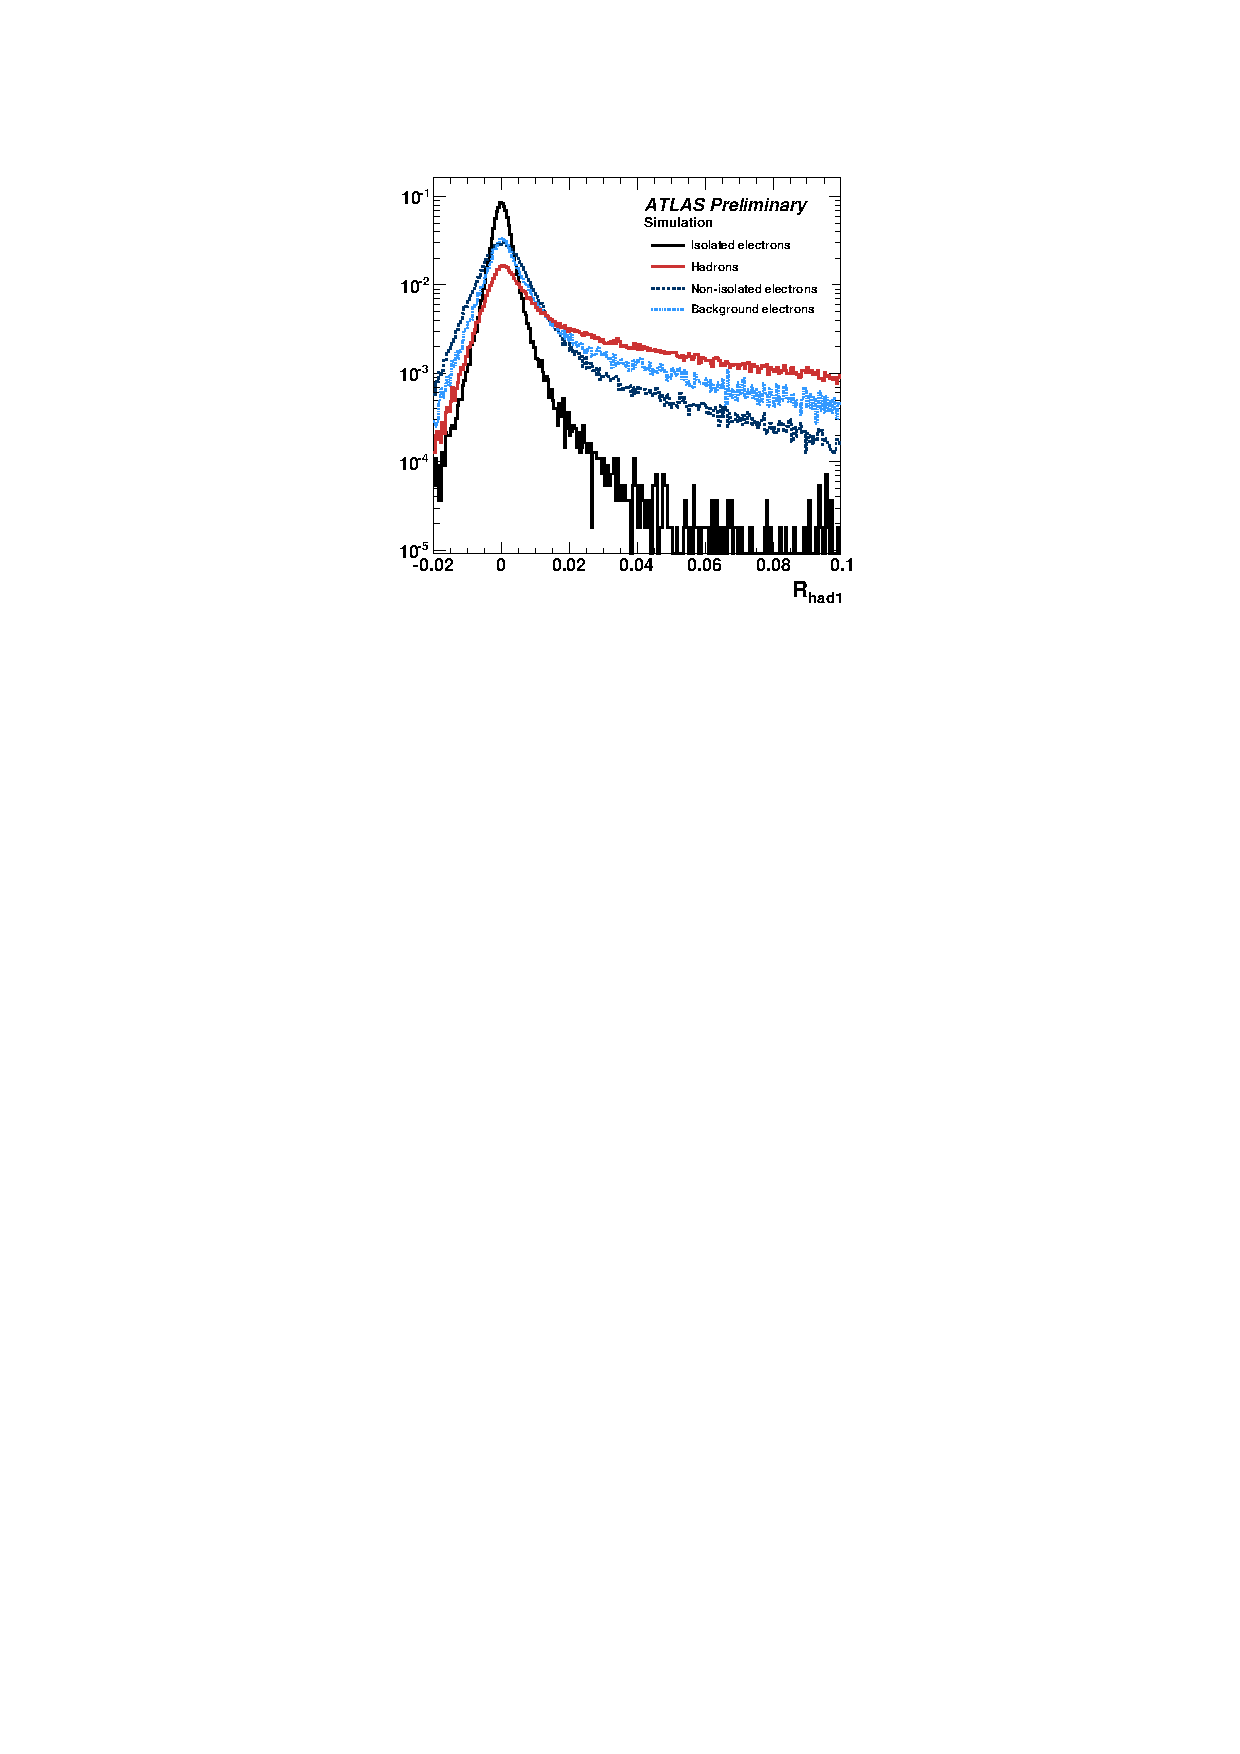
\includegraphics[width=0.2\textwidth]{imagens/egamma_padrao/egamma_padrao_rhad1.pdf}
        }
        \subfigure[\protect\acrshort{weta2}.]{%
            \label{fig:weta2}
            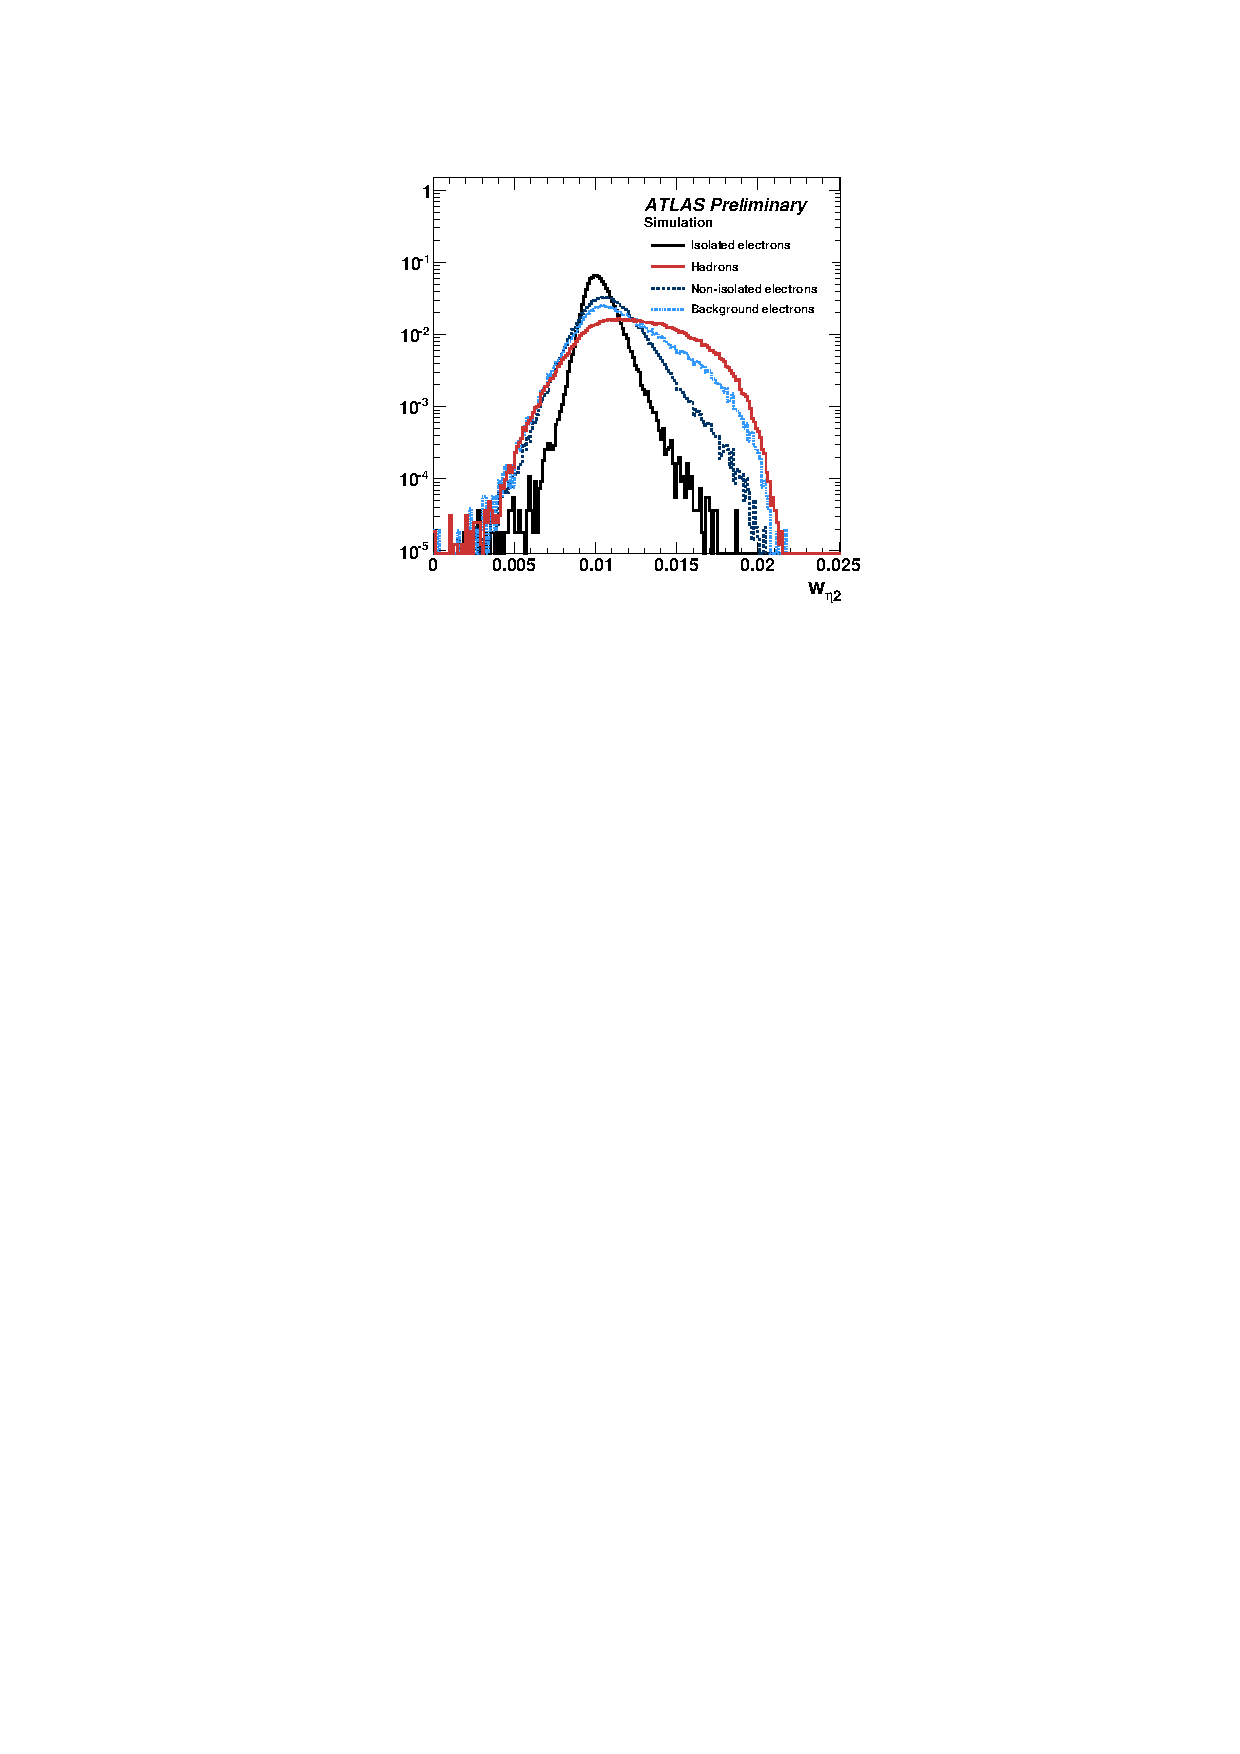
\includegraphics[width=0.2\textwidth]{imagens/egamma_padrao/egamma_padrao_weta2.pdf}
        }
        \subfigure[\protect\acrshort{reta}.]{%
            \label{fig:reta}
            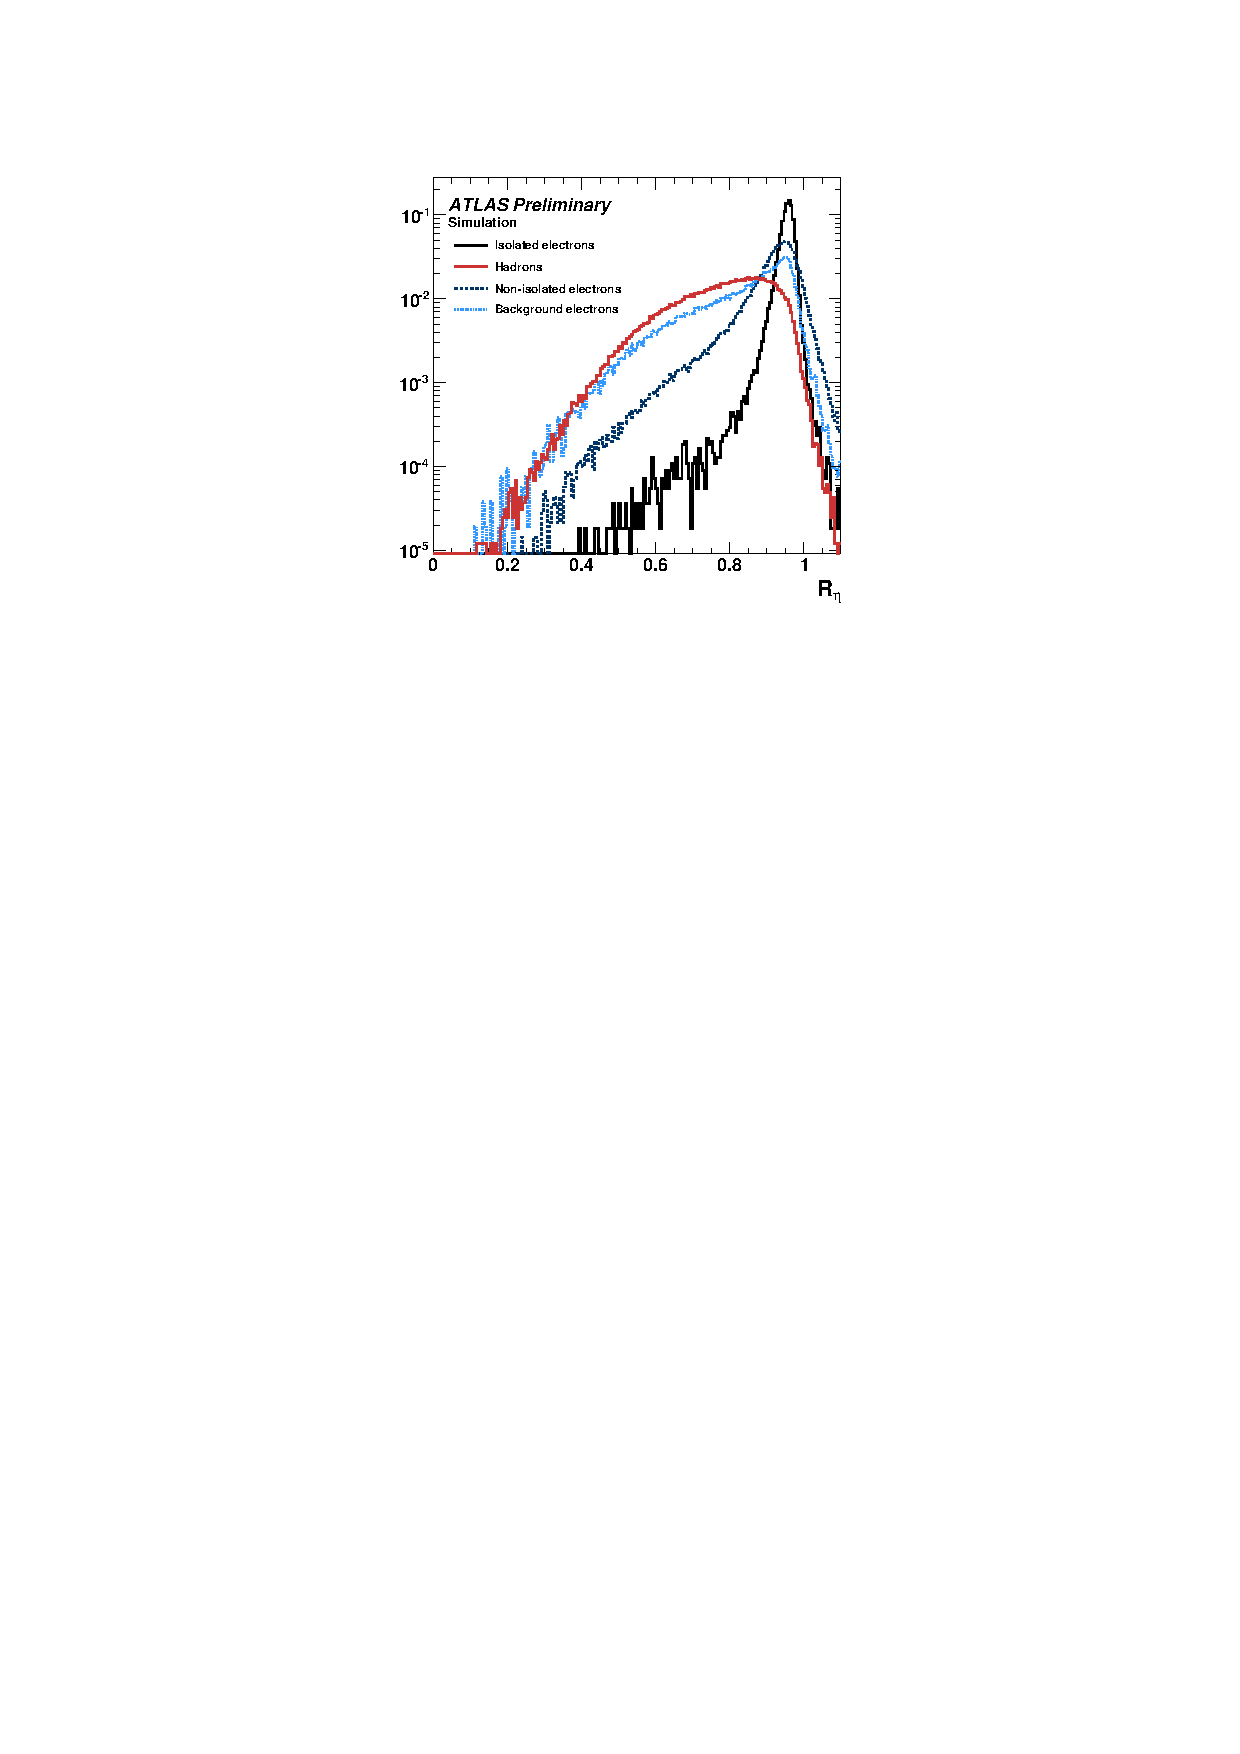
\includegraphics[width=0.2\textwidth]{imagens/egamma_padrao/egamma_padrao_reta.pdf}
        }
        \subfigure[\protect\acrshort{wstot}.]{%
            \label{fig:wstot}
            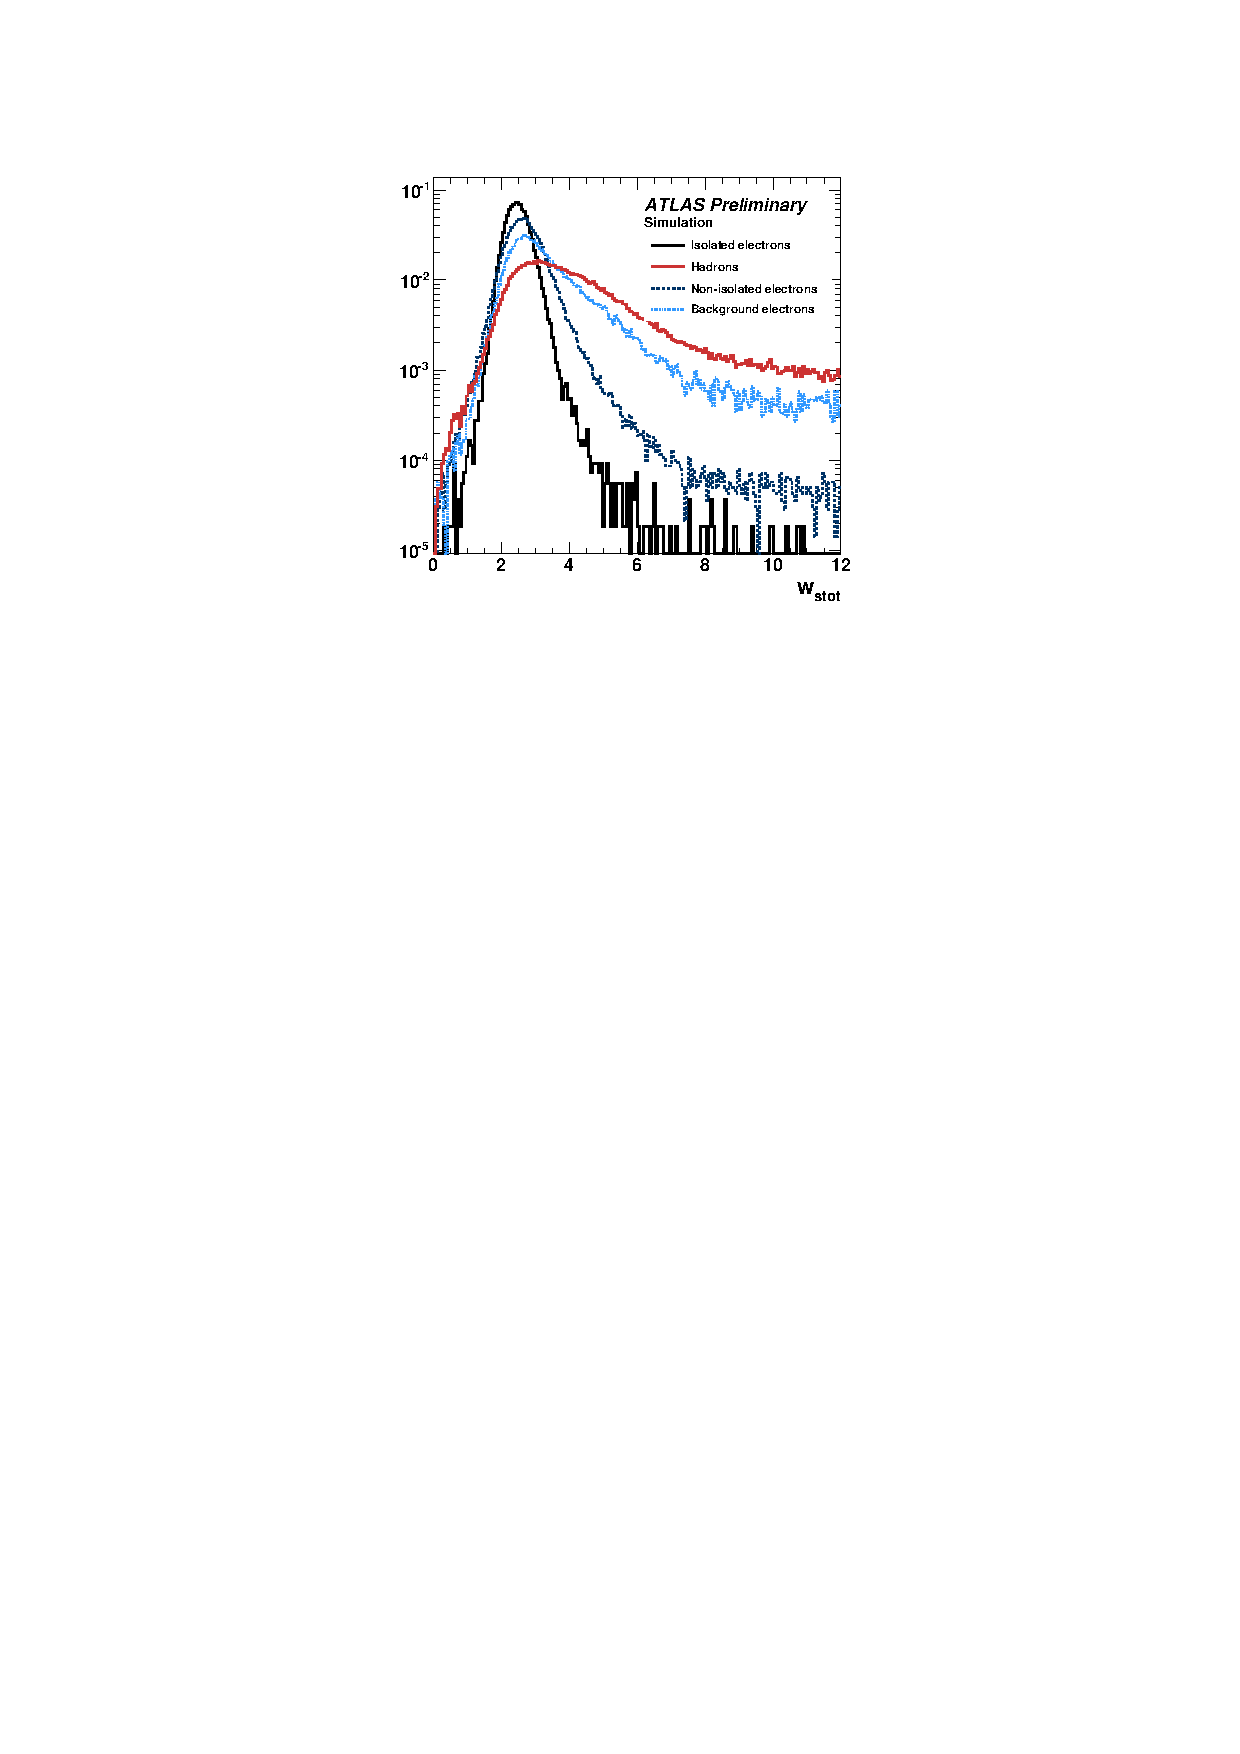
\includegraphics[width=0.2\textwidth]{imagens/egamma_padrao/egamma_padrao_wstot.pdf}
        }\\
        \subfigure[\protect\acrshort{eratio}.]{%
            \label{fig:eratio}
            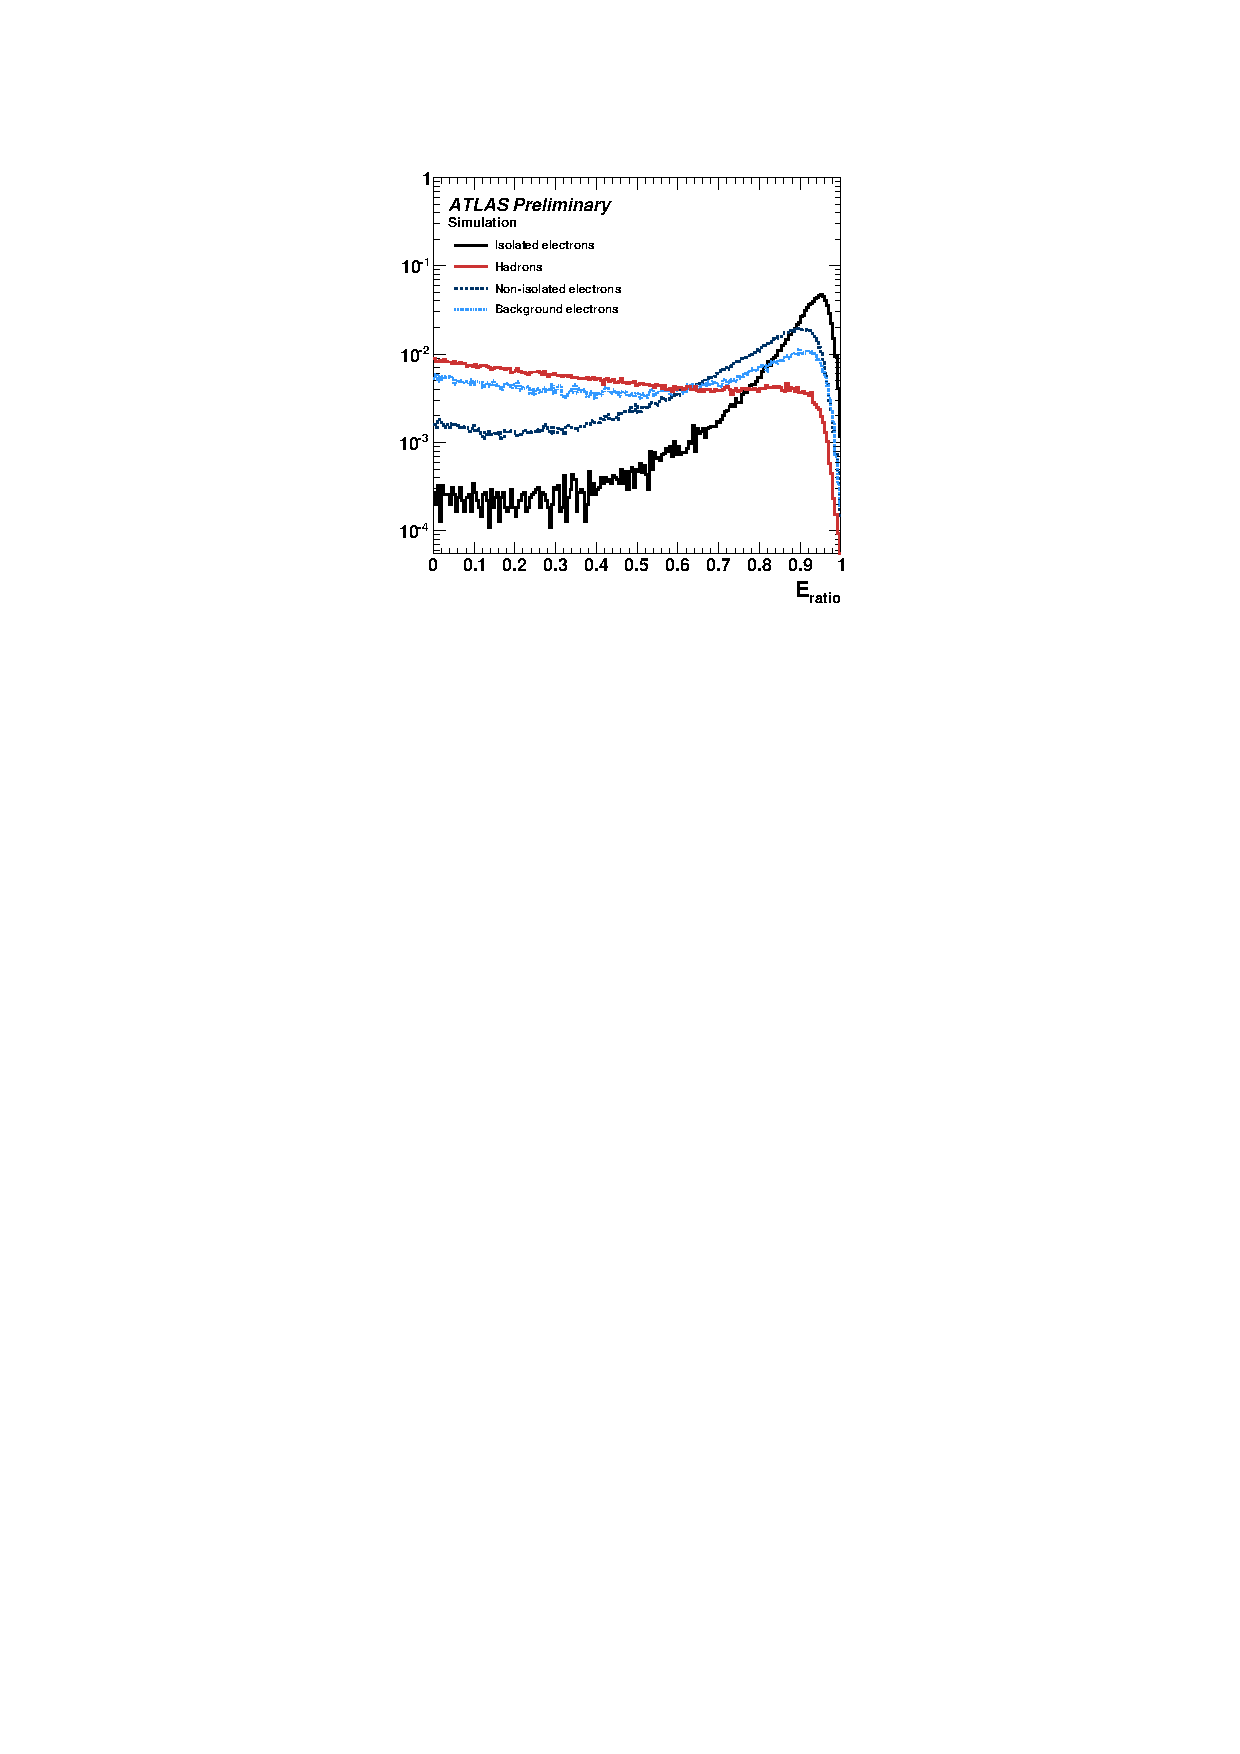
\includegraphics[width=0.2\textwidth]{imagens/egamma_padrao/egamma_padrao_eratio.pdf}
        }
        \subfigure[\protect\acrshort{d0}.]{%
            \label{fig:d0}
            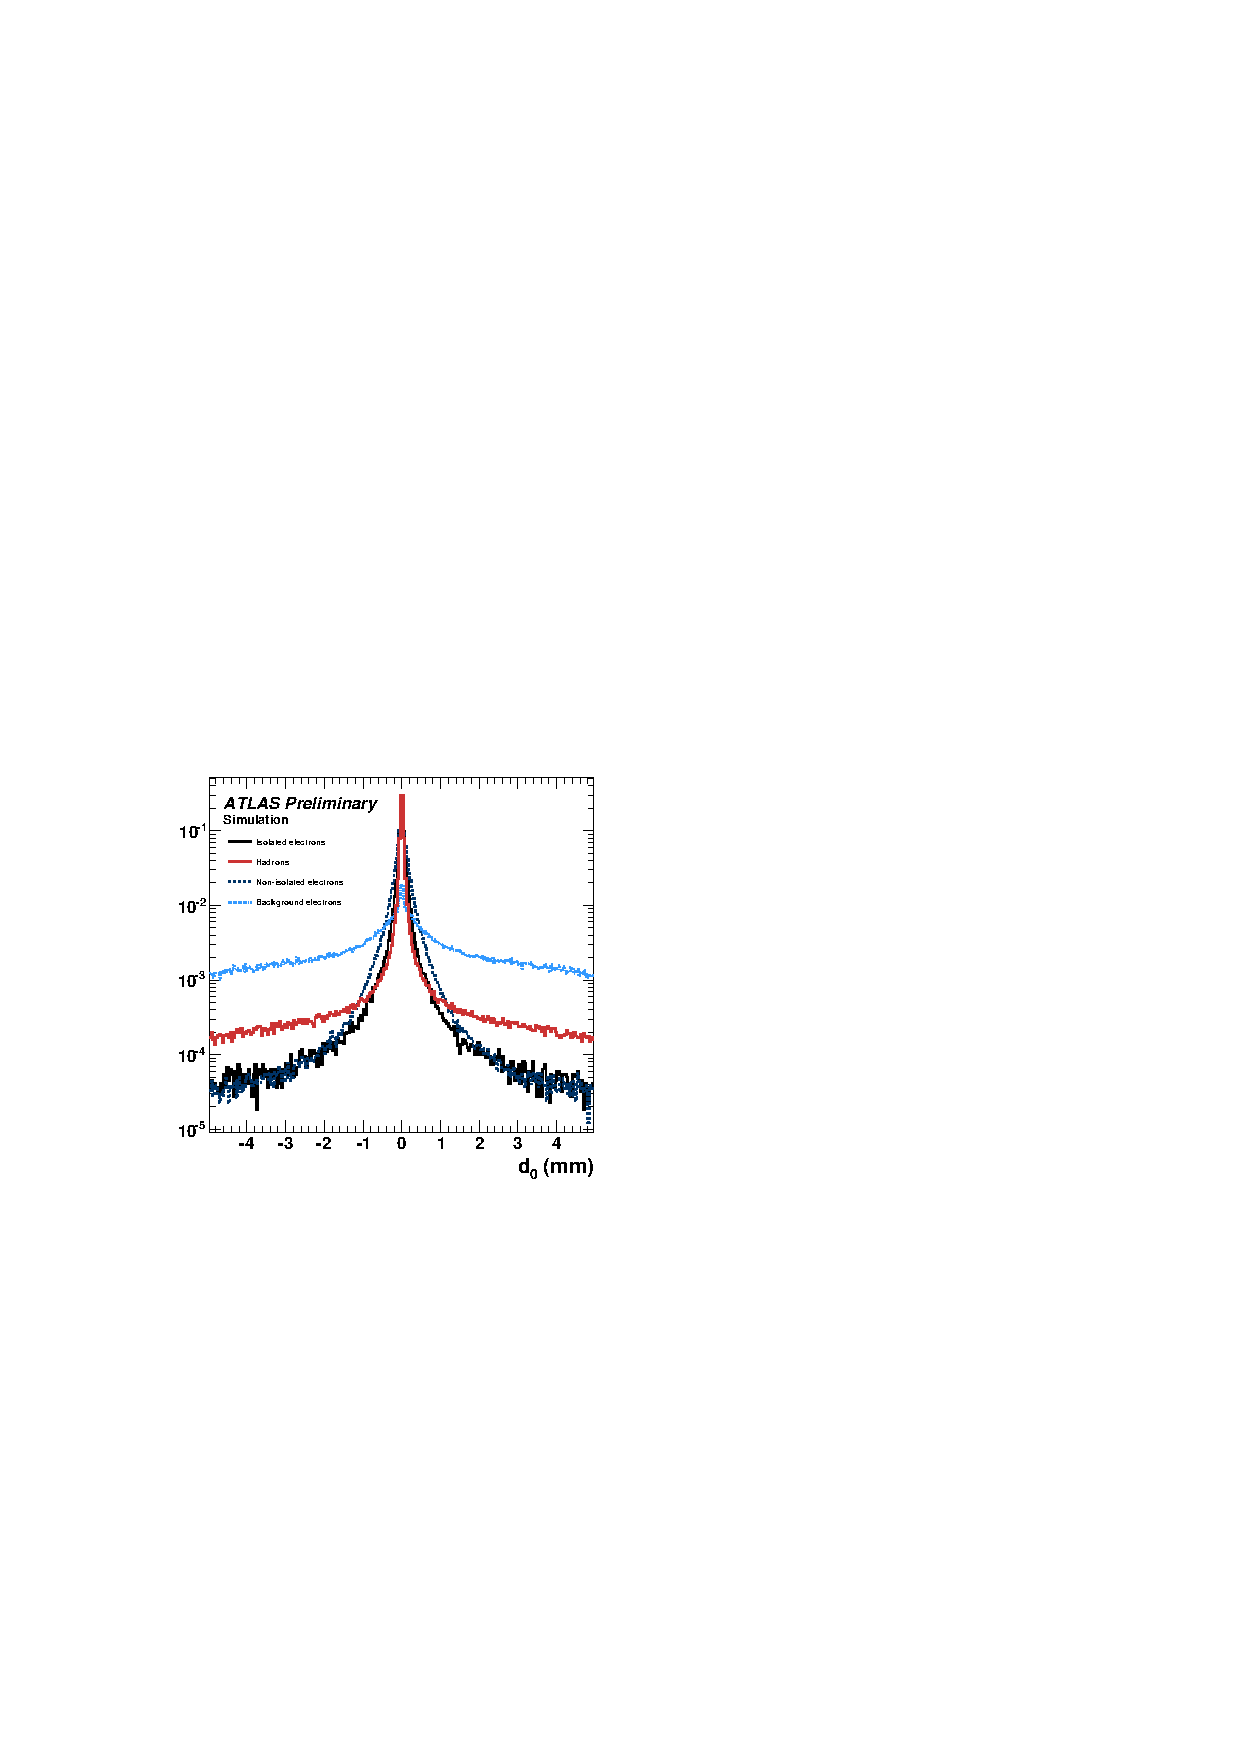
\includegraphics[width=0.2\textwidth]{imagens/egamma_padrao/egamma_padrao_d0.pdf}
        }
        \subfigure[\protect\acrshort{deta1}.]{%
            \label{fig:deta1}
            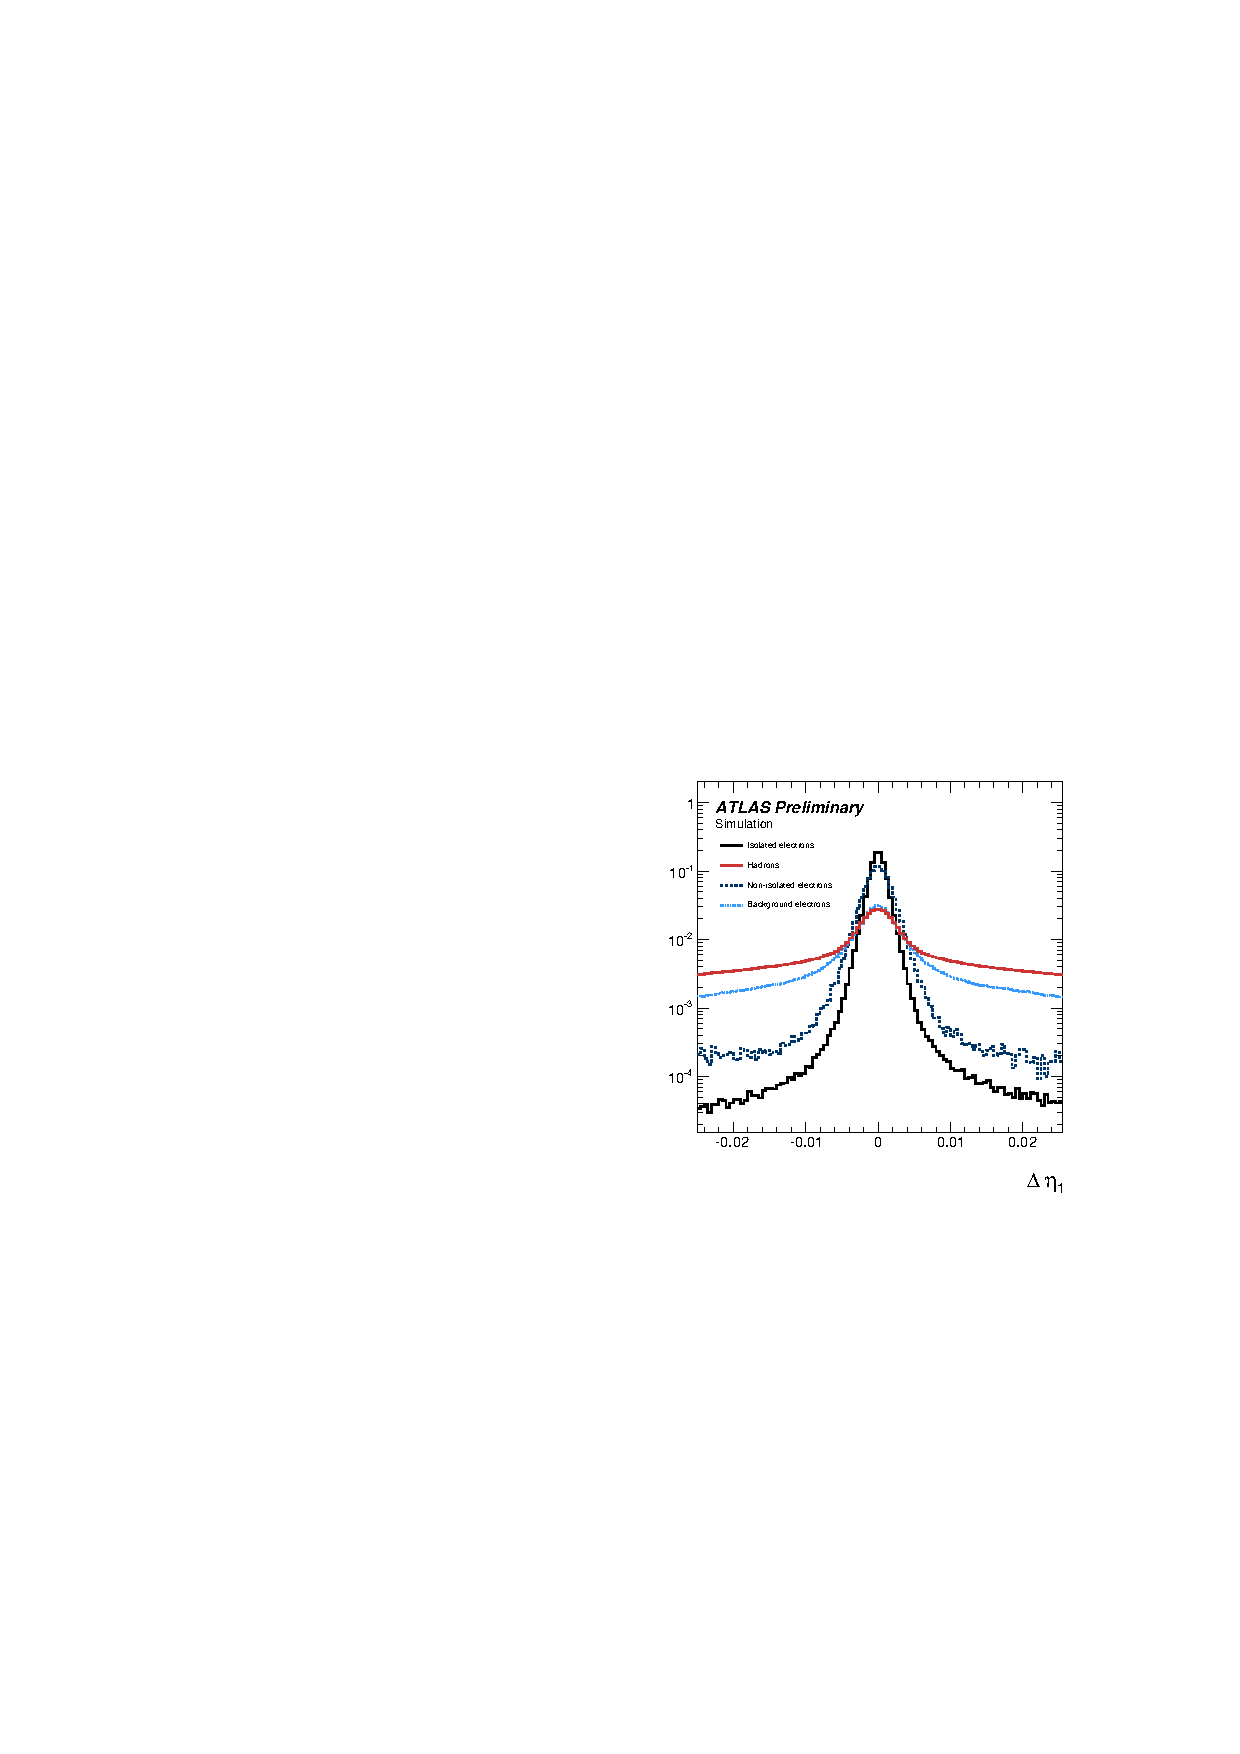
\includegraphics[width=0.2\textwidth]{imagens/egamma_padrao/egamma_padrao_deltaeta1.pdf}
        }
        \subfigure[\protect\acrshort{Ep}.]{%
            \label{fig:Ep}
            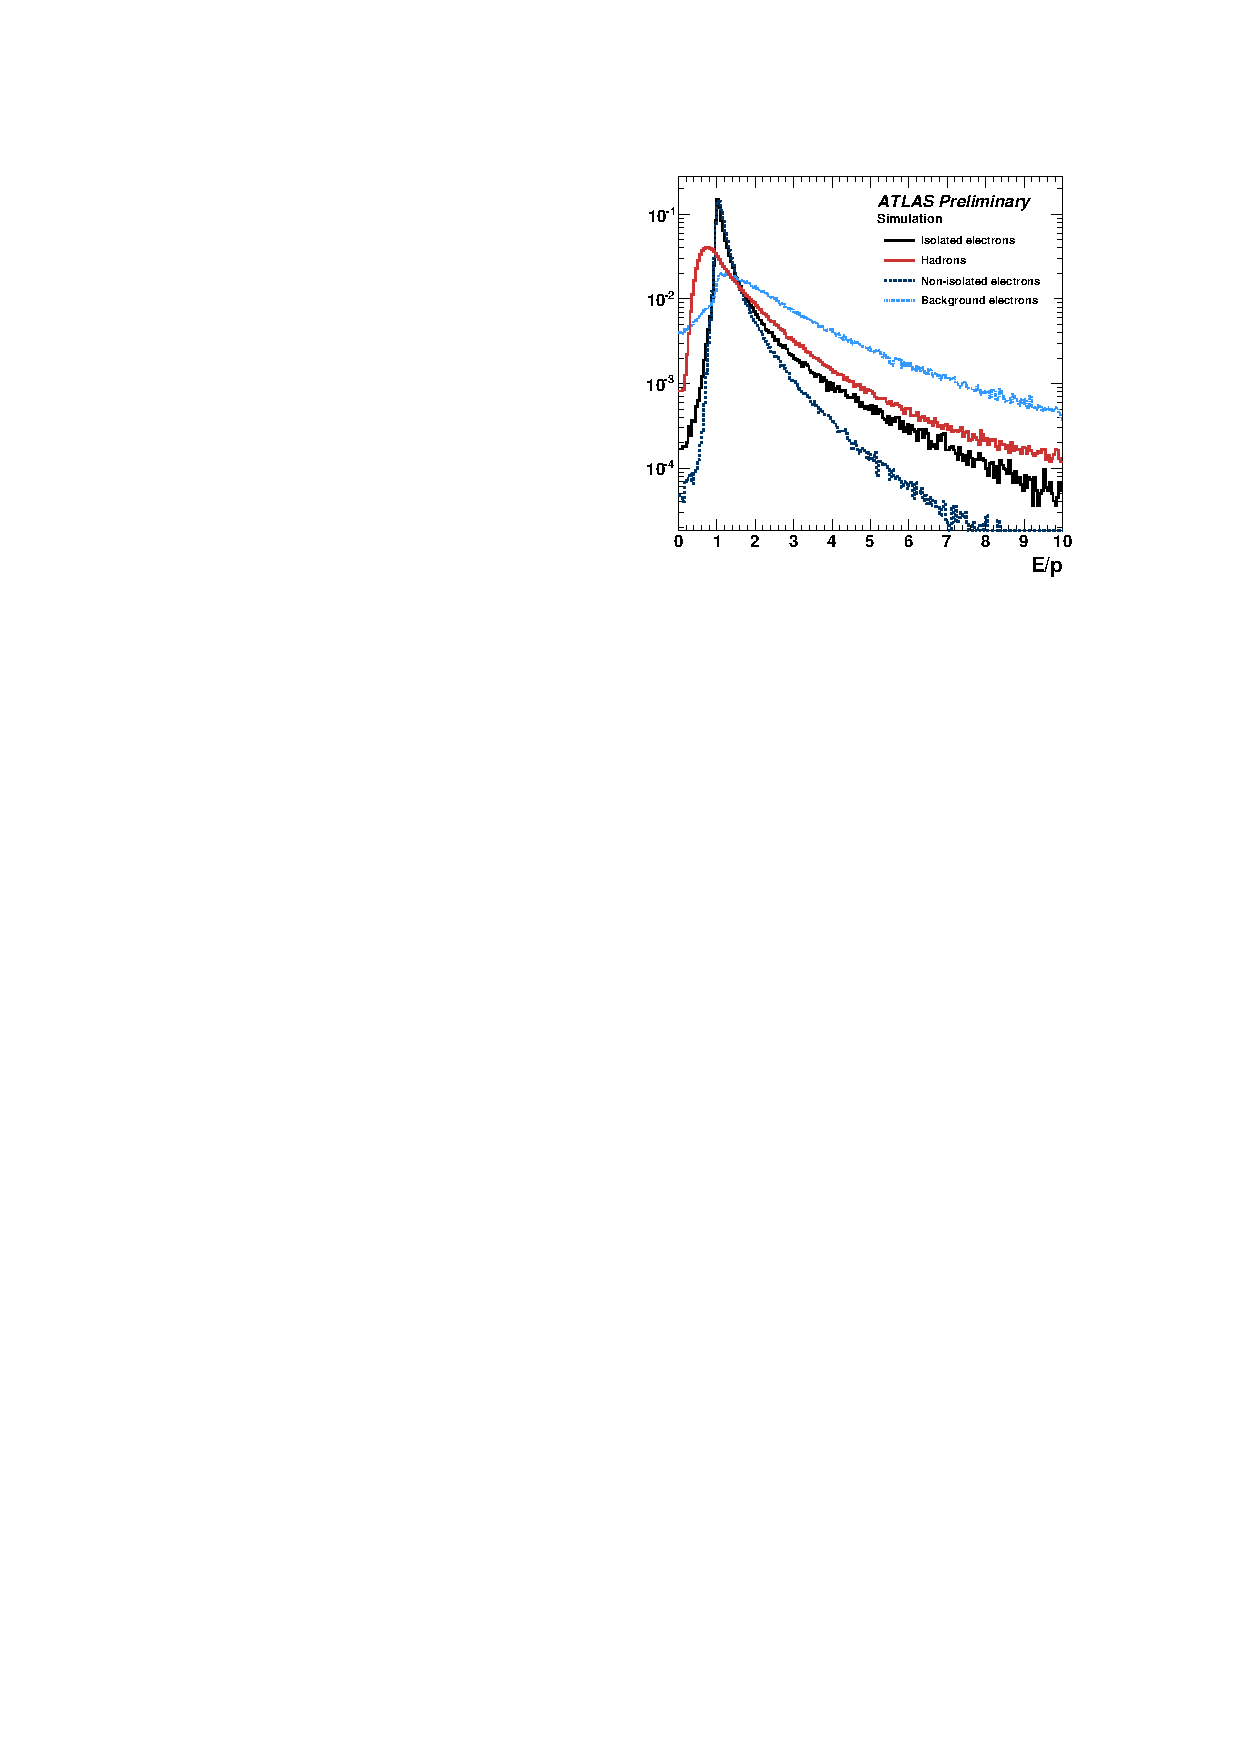
\includegraphics[width=0.2\textwidth]{imagens/egamma_padrao/egamma_padrao_ep.pdf}
        }
\caption[Distribuição de elétrons e seu ruído físico para algumas das variáveis
dos algoritmos e/$\gamma$ padrões.]
{Distribuição de elétrons e seu ruído físico para algumas das variáveis
dos algoritmos e/$\gamma$ padrões. Em preto, elétrons isolados; em vermelho,
hádrons; em azul escuro pontilhado, elétrons não-isolados; e em azul claro
pontilhado, elétrons constituintes de ruído. Extraído de \cite{expected_perf_2011}.}
\label{fig:cortes_egamma_padrao}
\end{sidewaysfigure}

É possível observar os diferentes comportamentos para cada uma das
categorias. Por exemplo, elétrons isolados na variável \gls{reta},
Figura~\ref{fig:reta}, possuem grande parte de valores próximos a 1, 
uma vez praticamente toda sua energia estará depositada no centro da 
\gls{roi}, por outro lado, hádrons distribuem sua energia em um espaço maior da
\gls{roi}, de forma que ao realizar a fração \gls{reta}, obterá-se geralmente
valores menores de 1. No caso da variável
\gls{eratio}, \ref{fig:eratio}, é esperado o mesmo valor para elétrons isolados,
onde a diferença de deposito entre as duas células de maior
energia deverá ser grande para elétrons, uma vez que os mesmos terão grande parte 
de sua energia depositada na célula de maior energia, e pequeno para os hádrons. Cada variável
tem sua distribuição especifica, mas reflete uma diferença física da interação
de hádrons e elétrons com o detector.


\subsection{HLT\_EgammaCaloRinger (HLT\_Ringer)}
\label{ssec:hlt_ringer}

\newacronym[type=Abrev,\glslongpluralkey={Redes Neurais Artificiais}]
{rna}{RNA}{Rede Neural Artificial}
\newacronym[type=Abrev]{ica}{ICA}{Análise de Componentes Independentes}
\newacronym[type=Abrev]{nlica}{NLICA}{Análise de Componentes Independentes
Não-Linear}
\newacronym[type=Abrev]{pca}{PCA}{Análise de Componentes Principais}
\newacronym[type=Abrev]{pcd}{PCD}{Componentes Principais de Discriminação}
\newacronym[type=Abrev]{som}{SOM}{Mapas Auto-Organizáveis}

Uma outra proposta para se identificar a evolução do chuveiro no calorímetro é 
abordada pelo algoritmo alternativo proposto, afim de se identificar as
partículas \gls{em}. Como o algoritmo é proposto para atuar sobre as variáveis
do calorímetro, ele não faz distinção de elétron e pósitrons para fótons, essa
distinção pode ser realizada posteriormente utilizando a informação do \gls{id}.
Inicialmente esse algoritmo, chamado de \gls{hltringer}, foi planejado para operar no
\acrlong{l2} como uma alternativa ao \gls{t2calo}, o ambiente mais restritivo 
em questões de tempo. Ao invés de gerar diversas variáveis de interpretação física 
para a compreensão da interação da partícula com o calorímetro, como os já
citados: \gls{eratio}, \gls{reta} e \gls{Rhad1}; o algoritmo utiliza a informação anelada
de calorimetria como o seu \gls{fex} (Tópico~\ref{sssec:anelamento}) 
e um processo de discriminação para o seu \gls{hypo}. Qualquer método estatístico 
pode ser aplicado para realizar o processo de discriminação. 
Em particular, os estudos deste trabalho utilizaram \glspl{rna} \cite{neural_networks} 
(Tópico~\ref{sssec:rna}), pois obtiveram melhor performance nos estudos
realizados no inicio do projeto.

Diversas técnicas de pré-processamento podem ser combinadas com redes neurais de
forma a melhorar a sua eficiência de discriminação. Estudos anteriores
\cite{tese_eduardo,tese_torres} utilizaram métodos como \gls{ica}, \gls{pca},
\gls{nlica}, \gls{som} e \gls{pcd}, obtendo resultados melhores que uma
abordagem utilizando diretamente \gls{rna}. Um caso especial de pré-processamento 
de dados, necessária quando utilizando redes neurais, é a normalização dos dados. Esse 
pré-processamento ajusta o alcance de energia dos anéis ao alcance dinâmico das
\gls{rna}. Uma grande gama de métodos de normalização são utilizados, podendo
gerar alterações no espaço de representação de anéis, de forma que a
interpretação da nova representação pode ter uma melhor, ou pior, interpretação
pela \gls{rna}. As normalizações testadas para otimizar a eficiência do
\gls{hltringer} estão explicadas no Tópico~\ref{sssec:preproc_norm}.

\subsubsection{O processo de anelamento}
\label{sssec:anelamento}

\begin{figure}[hp!]
\label{fig:cons_aneis}
\centering
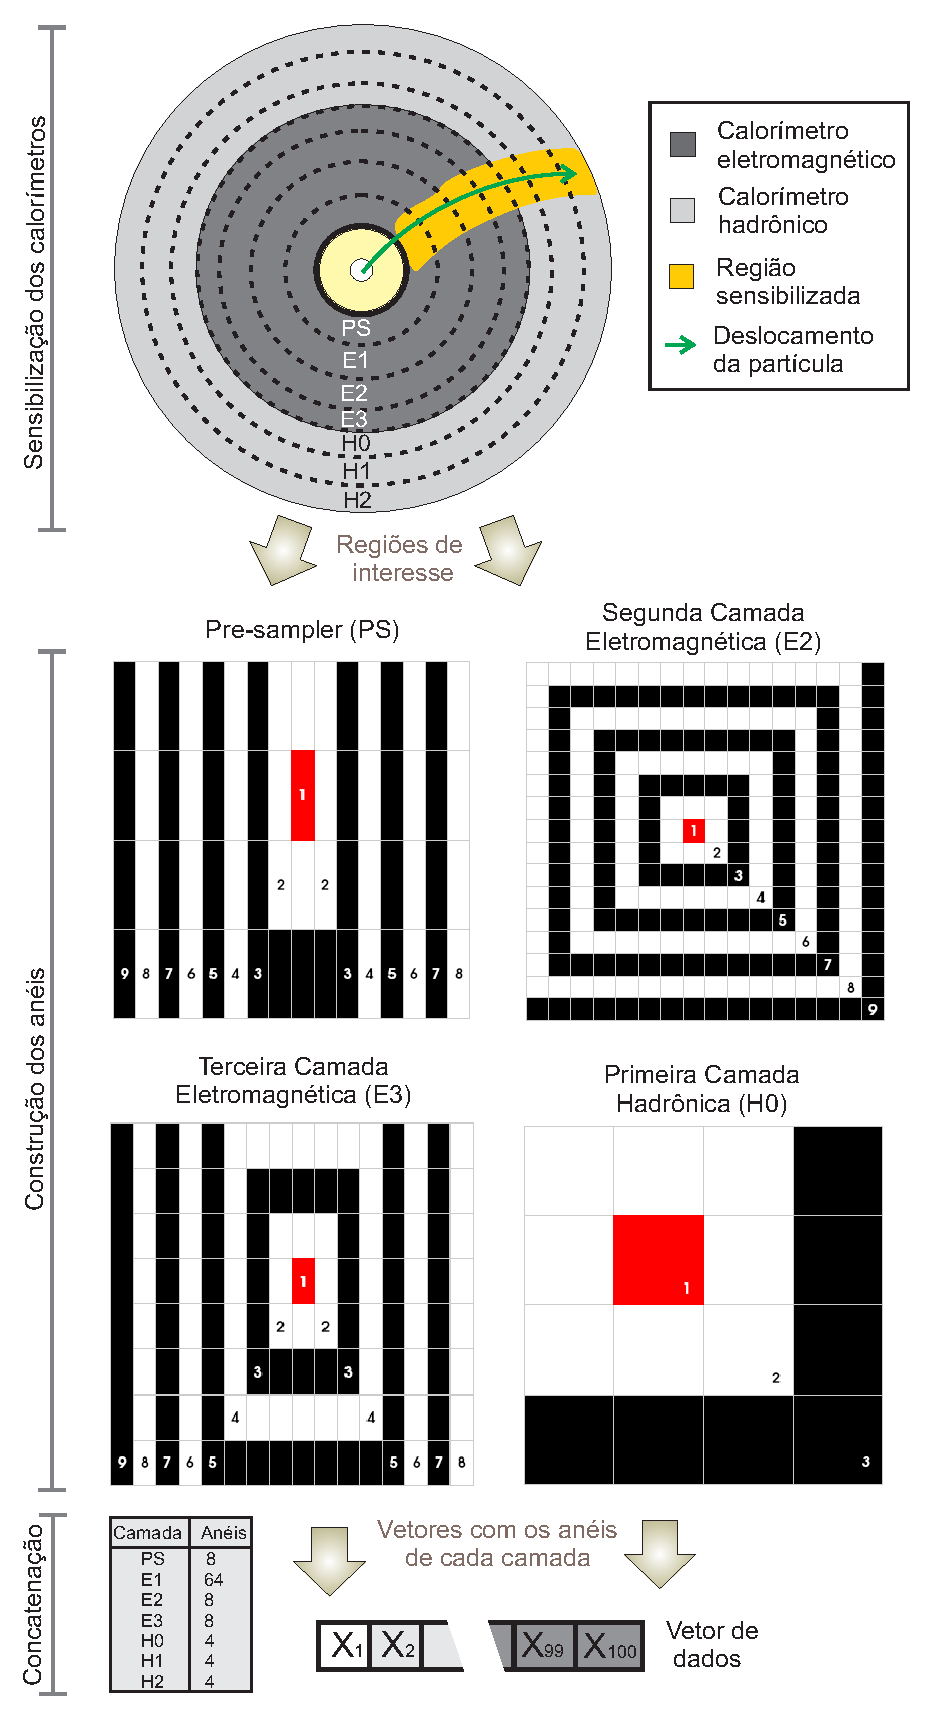
\includegraphics[height=0.9\textheight]{imagens/cons_aneis.pdf}
\caption[Diagrama do processo de construção dos anéis.]
{Diagrama do processo de construção dos anéis. Extraído de \cite{tese_eduardo}.}
\end{figure}

O processo de anelamento, esboçado na Figura~\ref{fig:cons_aneis}, é realizado
para todas as camadas (\gls{ps}, \gls{e1}, \gls{e2}, \gls{e3}, \gls{h0},
\gls{h1} e \gls{h2}) do Sistema de Calorimetria do \gls{atlas}. Como foi dito,
no \gls{l2} a semente utilizada para a construção do aglomerado é a célula quente  -- ou a célula mais
energética -- da \gls{e2} na \gls{roi} gerada a partir da posição 
fornecida pelo \gls{l1}. No \gls{hltringer}, ao invés da construção do
aglomerado, é realizada a construção de anéis concêntricos, onde essa célula
será o núcleo, e sua energia a informação contida no primeiro anel, o anel central. 
Os anéis posteriores contêm a soma da energia das células adjacentes
exteriores ao anel anterior, por exemplo, no caso do segundo anel, as células imediatamente
exteriores a célula quente. Esse processo irá se repetir até que uma região pré-determinada seja
completamente preenchida. Atualmente o valor utilizado é de $0,4\times0,4$ em
$\Delta\eta\times\Delta\phi$. Nas outras camadas, a posição da
semente é utilizada para encontrar a célula central e o processo é repetido, até
que a mesma região seja preenchida, entretanto, como a granularidade das células
do calorímetro variam conforme a segmentação longitudinal, o número de anéis variam
para cada camada. O conceito de anéis é abstrato: como o \gls{l2} calcula
um novo centro na \gls{roi} formada a partir da informação fornecida pelo
\gls{l1}, anéis podem por ventura necessitar de células exteriores a \gls{roi},
e essas, não estando disponíveis para o \gls{l2}, geram anéis incompletos,
como aqueles ilustrados para o \gls{ps} a partir do terceiro anel. 
No caso de nenhuma célula estiver disponível para um dado anel, é então atribuído valor
nulo ao mesmo para garantir que o processo complete o número necessário no
preenchimento da região. Os anéis esboçados na figura são meramente
ilustrativos, não possuindo a proporção real para cada uma das camadas, nem o
número de anéis totais para cada uma delas. Um total de 100 anéis foram 
especificados inicialmente, divididos conforme as camadas da maneira indicada na
tabela contida no final dessa figura. Note que a quantidade de anéis é proporcional 
a granularidade de cada camada. Em uma discriminação não-segmentada
(veja~\ref{sssec:rna}), os anéis são concatenados em um grande vetor de dados,
como indicado.

O processo de anelamento reduz a quantidade de informação a ser analisada no
calorímetro, ao se agrupar diversas células em uma única informação, reduzindo
as $\sim$1000 células dentro da \gls{roi} em 100 anéis, ou seja, um fator de
compactação de $\sim$10$\times$. Indo além, o número total de anéis a serem
propagados para o método de discriminação pode ser reduzido através de estudo
com quantidade elevada de estatística do processo. Entretanto, a redução de informação 
é utilizada para se referir a compactação da
informação das células do calorímetro nos anéis, não podendo se comparar 
com a ordem de informação armazenada nas variáveis físicas, 
que se resumem a cerca de 5 variáveis.

Ao mesmo tempo, a interpretação física da propagação do
chuveiro é mantida, como a sua espessura lateral e profundidade longitudinal. 
Na Figura~\ref{fig:perfil_aneis} está um 
exemplo da deposição de energia de elétrons e de um dos hádrons que
compõem os jatos hadrônicos\footnote{Para evitar a repetição, quando se
referindo a jatos no Canal \gls{eg}, estará se mencionando os hádrons individuais
que formam os jatos hadrônicos, e não o conjunto. O canal de reconstrução de
jatos, diferente do Canal \gls{eg}, reconstrói o jato como um todo, 
o que pode gerar confusão na nomenclatura.} para a \gls{e2}. Pode-se observar na parte
superior da figura a deposição de energia nas células do calorímetro, onde os
jatos possuem um perfil de deposição mais largo, como o esperado para o chuveiro
dessas partículas, quando em comparação com a deposição de energia de um
elétron. Este, por sua vez, tem sua deposição de energia concentrada no centro da
\gls{roi}. A parte inferior, contendo a deposição de energia nos anéis formados 
para cada um dos caso, demonstra a diferença de ambos, onde elétrons depositam grande parte de
sua energia no primeiro anel, e pouca energia nos anéis mais externos, enquanto
os jatos possuem um perfil mais disperso, alcançando anéis mais externos.

\begin{figure}[ht!]
\label{fig:perfil_segunda_camada}
\centering
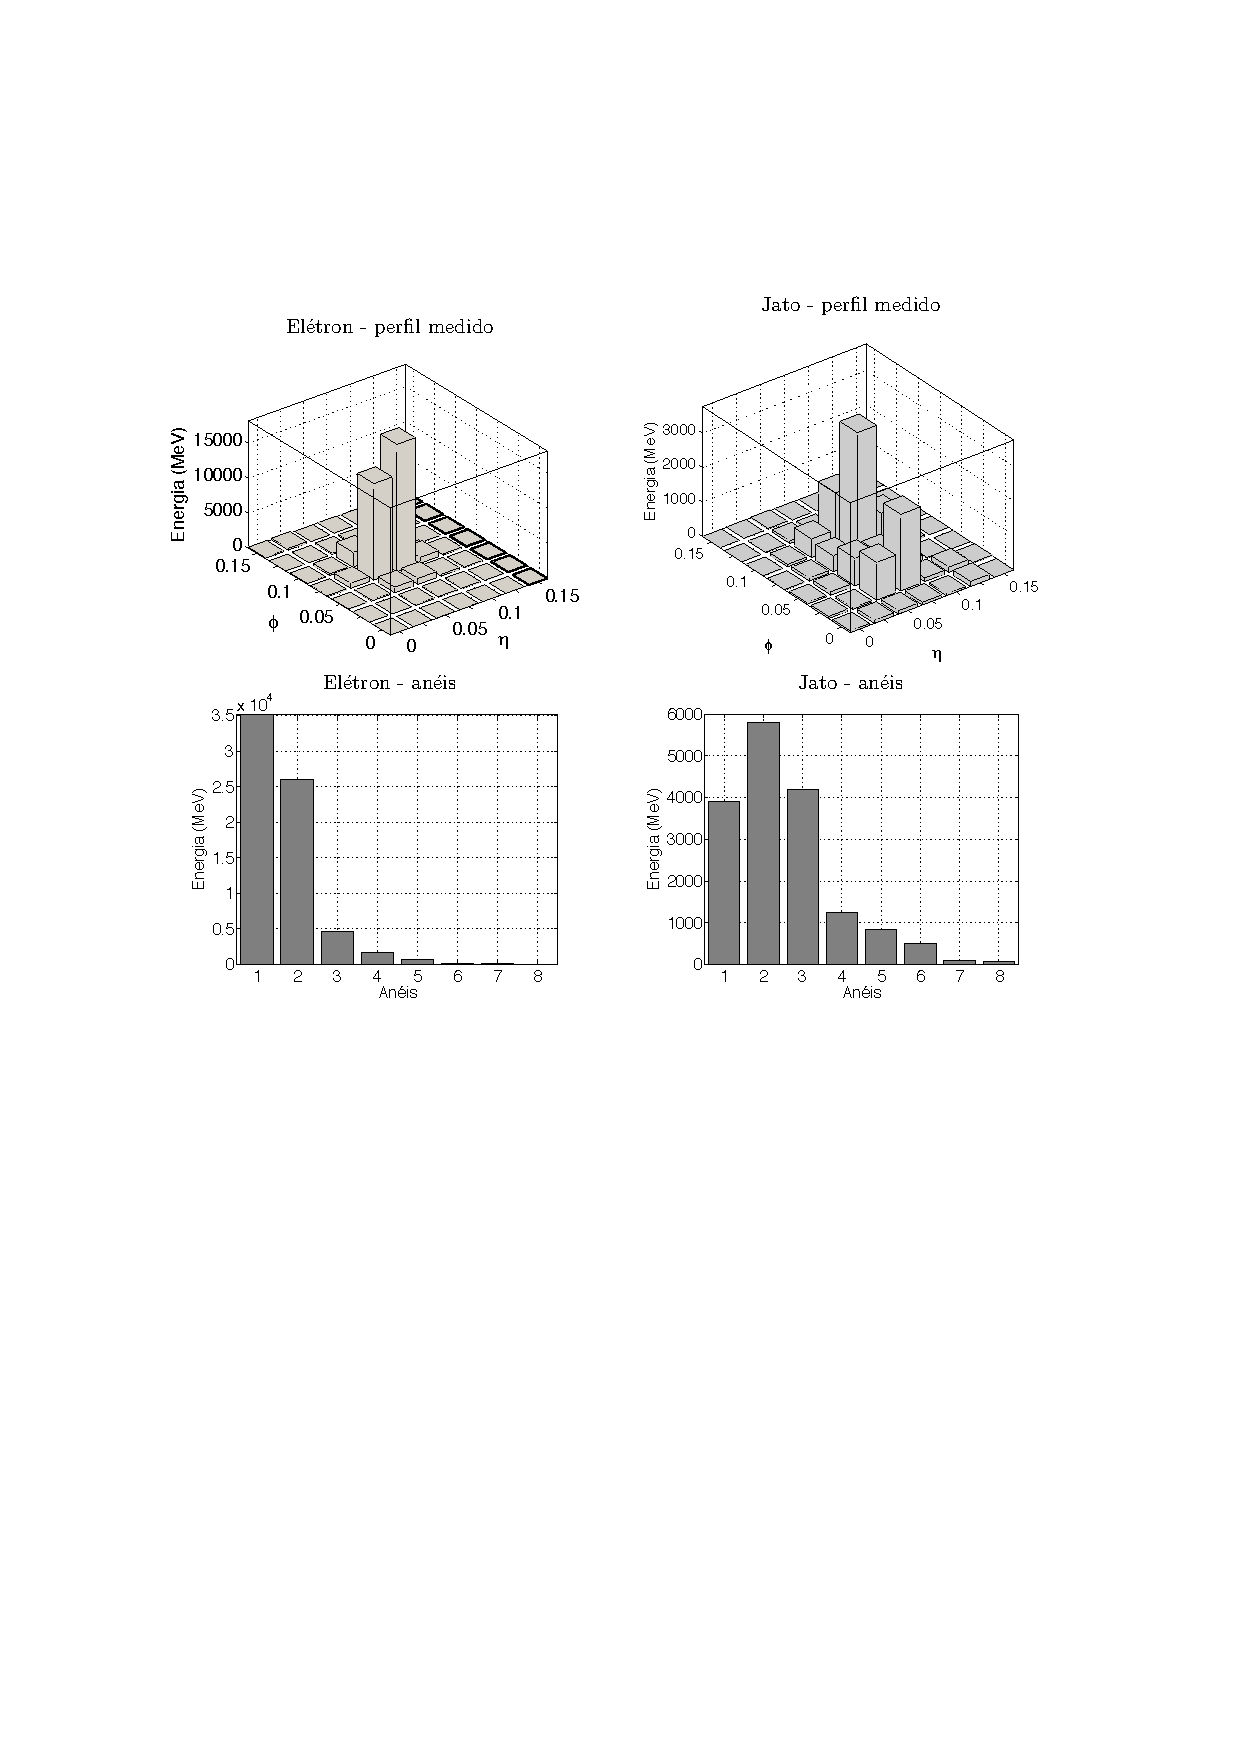
\includegraphics[width=0.9\textwidth]{imagens/segunda_camada_celulas.pdf}
\caption[Perfil de distribuição de energia nas células e anéis na segunda camada para 
elétrons e jatos.]{Perfil de distribuição de energia nas células e anéis na segunda camada 
para elétrons e jatos. Extraído de \cite{tese_eduardo}.}
\end{figure}

Quando considerando a distribuição de energia em anéis de uma maneira global,
pode-se observar a diferença dos perfis dos chuveiros \gls{em} e
\gls{had}. A Figura~\ref{fig:perfil_aneis} contém o perfil dos 100 anéis para um
elétron (\ref{fig:perfil_aneis_eletron}) e um jato
(\ref{fig:perfil_aneis_jato}), onde a distribuição citada para elétrons e jatos
na \gls{e2} se repete para as outras camadas do \gls{ecal}, com os jatos
distribuindo sua energia nos anéis mais externos. Por outro lado, os elétrons
geralmente não alcançam as camadas hadrônicas, sendo absorvidos pela
\gls{e2} ou \gls{e3}, enquanto jatos ultrapassam o \gls{ecal} depositando
energia no \gls{hcal}. Contudo, esse fato nem sempre é verdadeiro, elétrons
muito energéticos podem acabar ultrapassando a \gls{e3} e depositando parte de
sua energia na \gls{h1}, e jatos podem também serem absorvidos no \gls{ecal},
como aquele ilustrado em \ref{fig:perfil_aneis_jato_conf}.

\begin{figure}[ht!]
\label{fig:perfil_aneis}
\centering
  \subfigure[]{%
      \label{fig:perfil_aneis_eletron}
      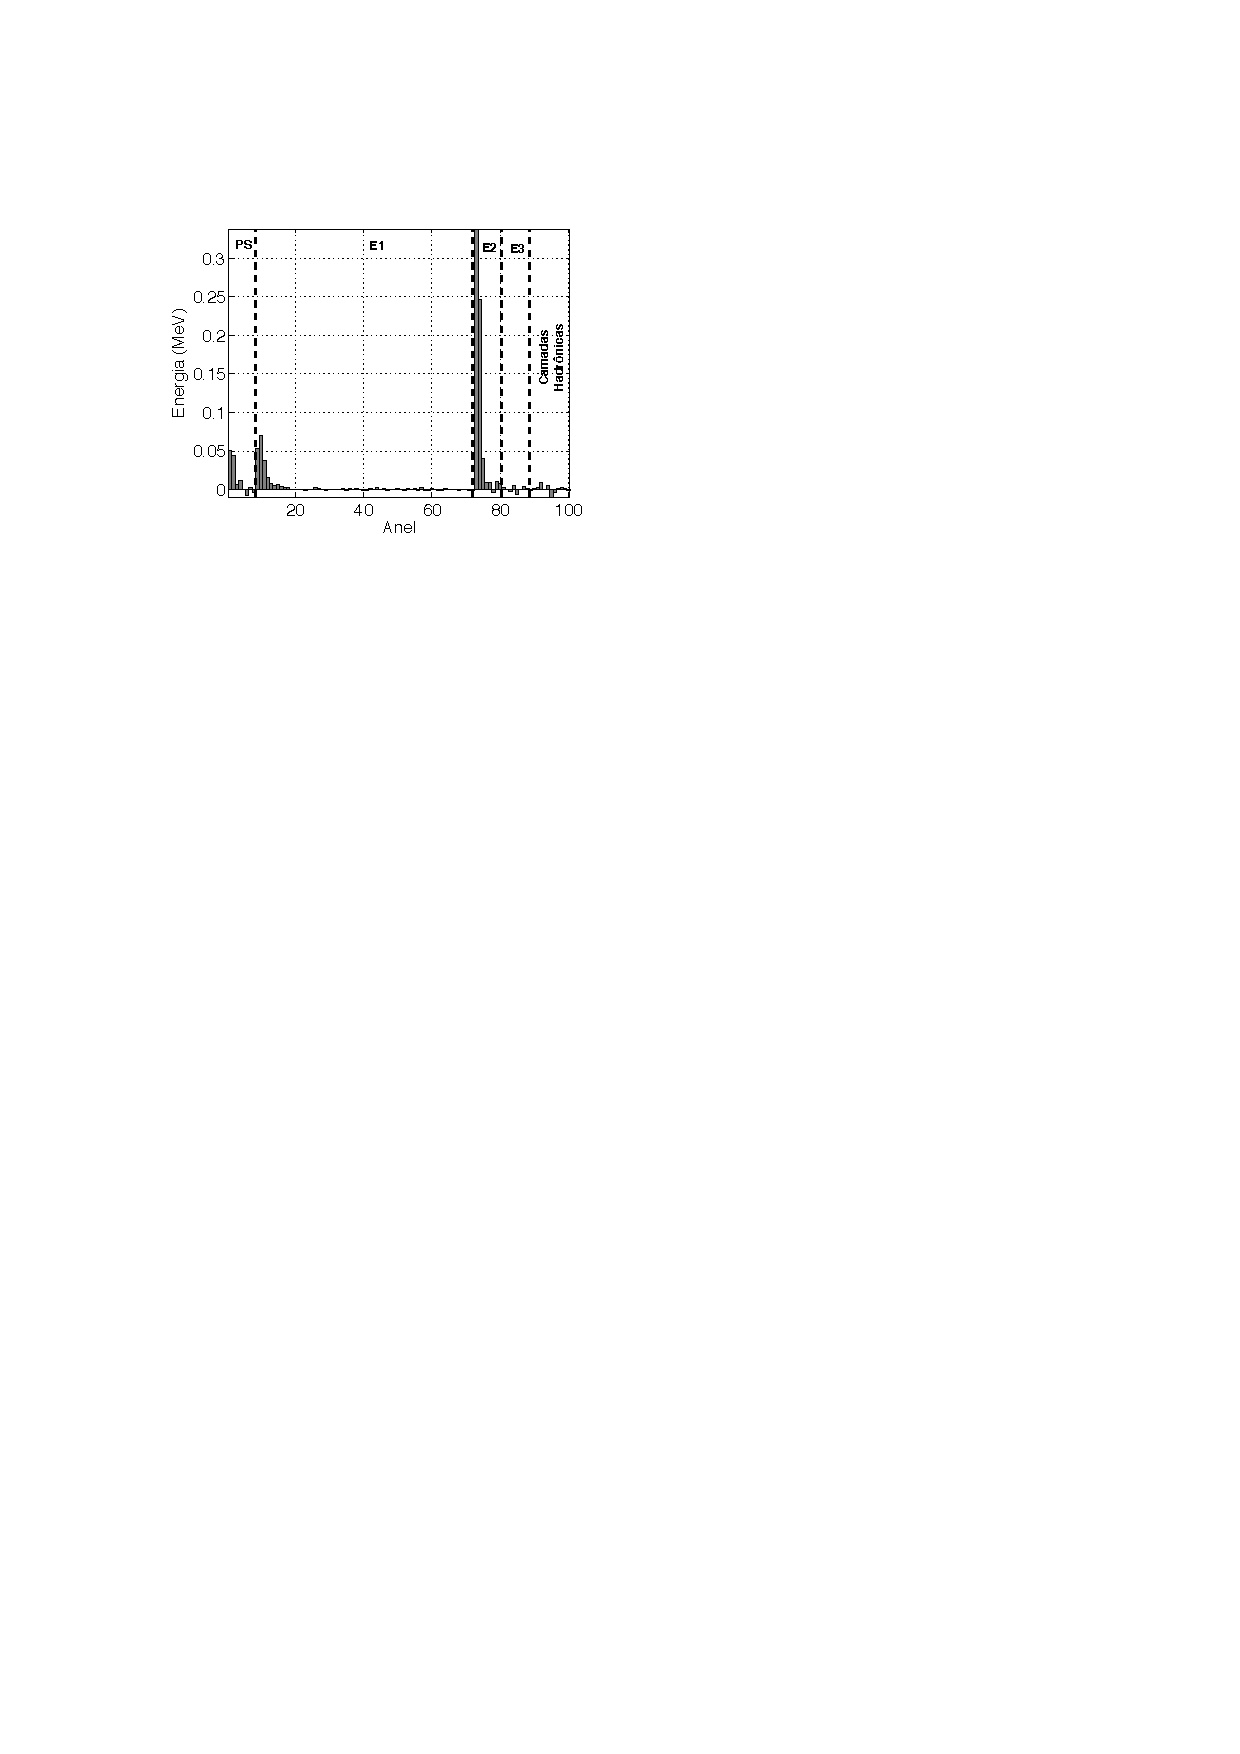
\includegraphics[width=0.45\textwidth]{imagens/perfil_aneis_eletron.pdf}
  }\hspace{0.01\textwidth}
  \subfigure[]{%
      \label{fig:perfil_aneis_jato}
      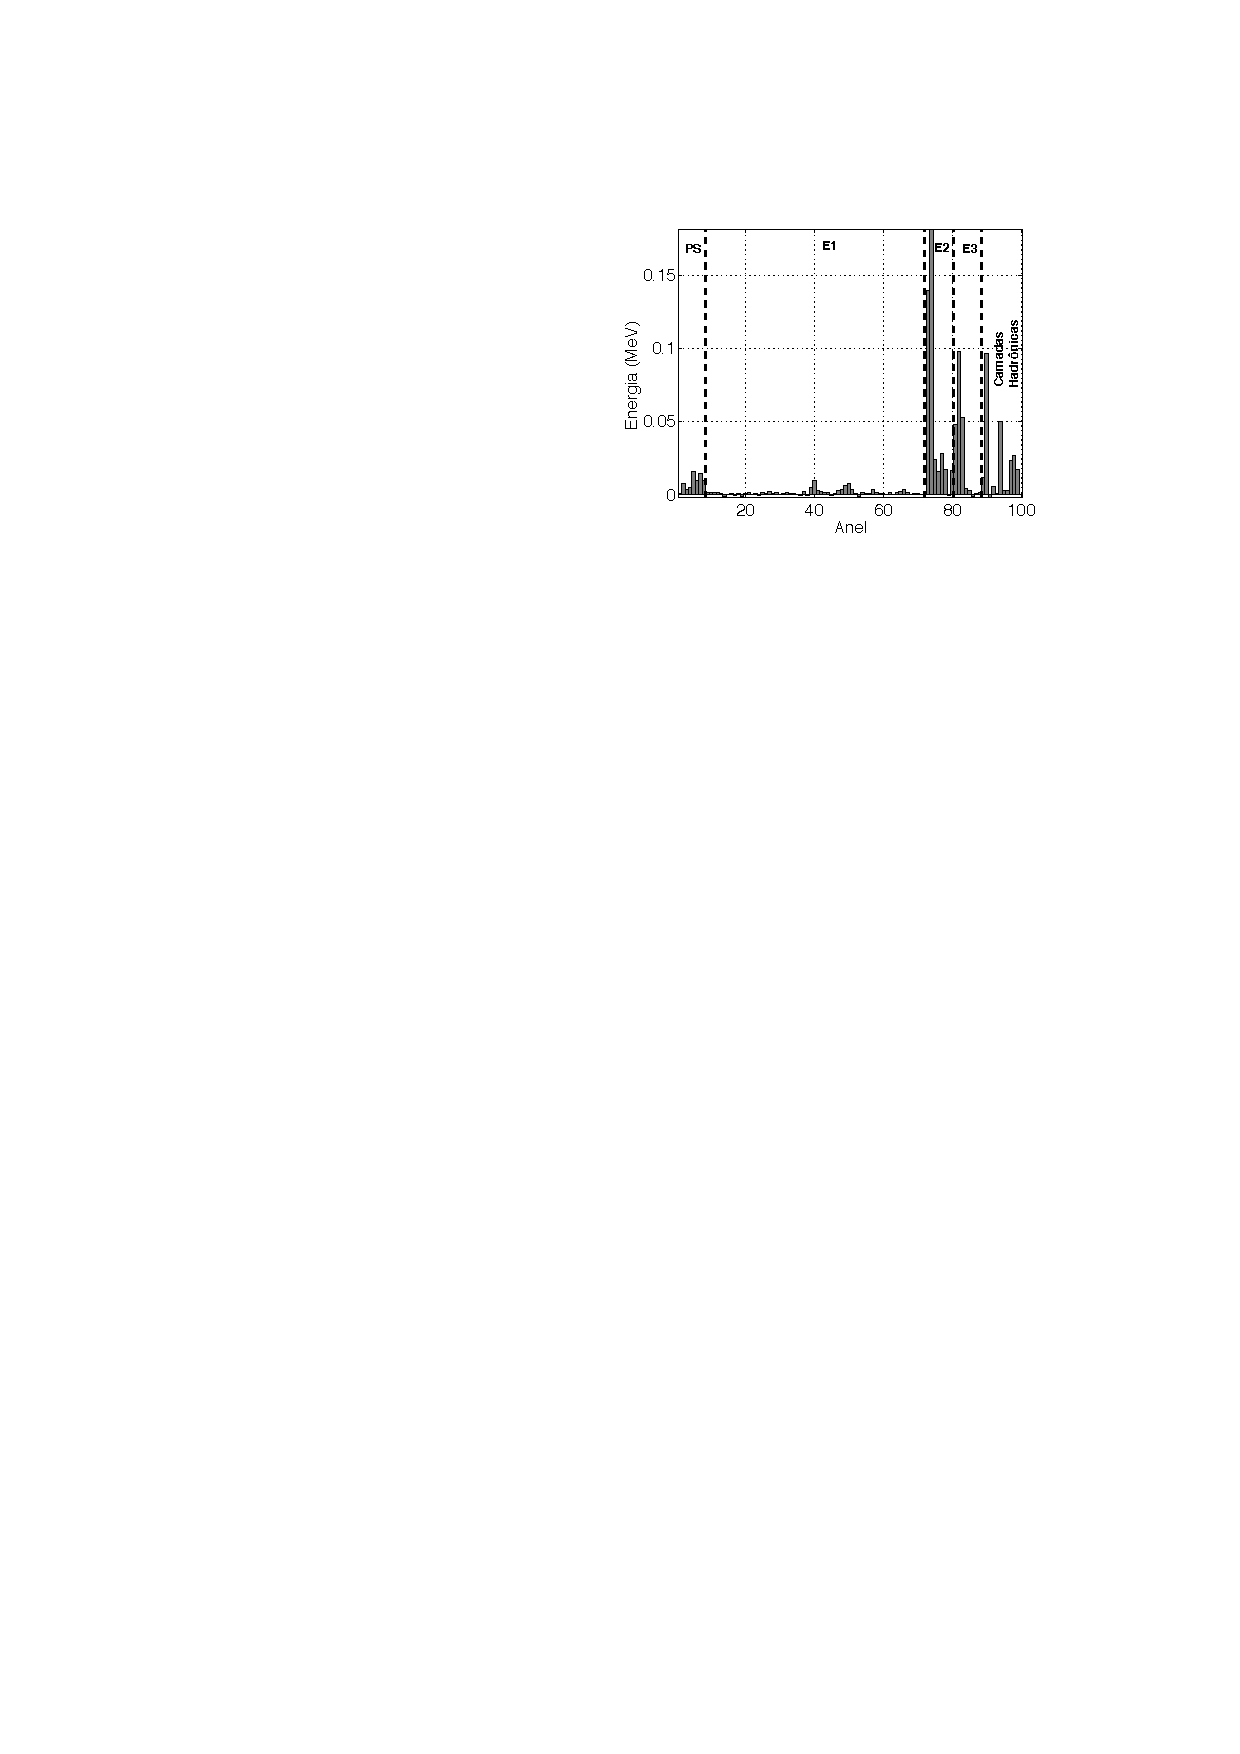
\includegraphics[width=0.45\textwidth]{imagens/perfil_aneis_jato.pdf}
  }\\
  \subfigure[]{%
      \label{fig:perfil_aneis_jato_conf}
      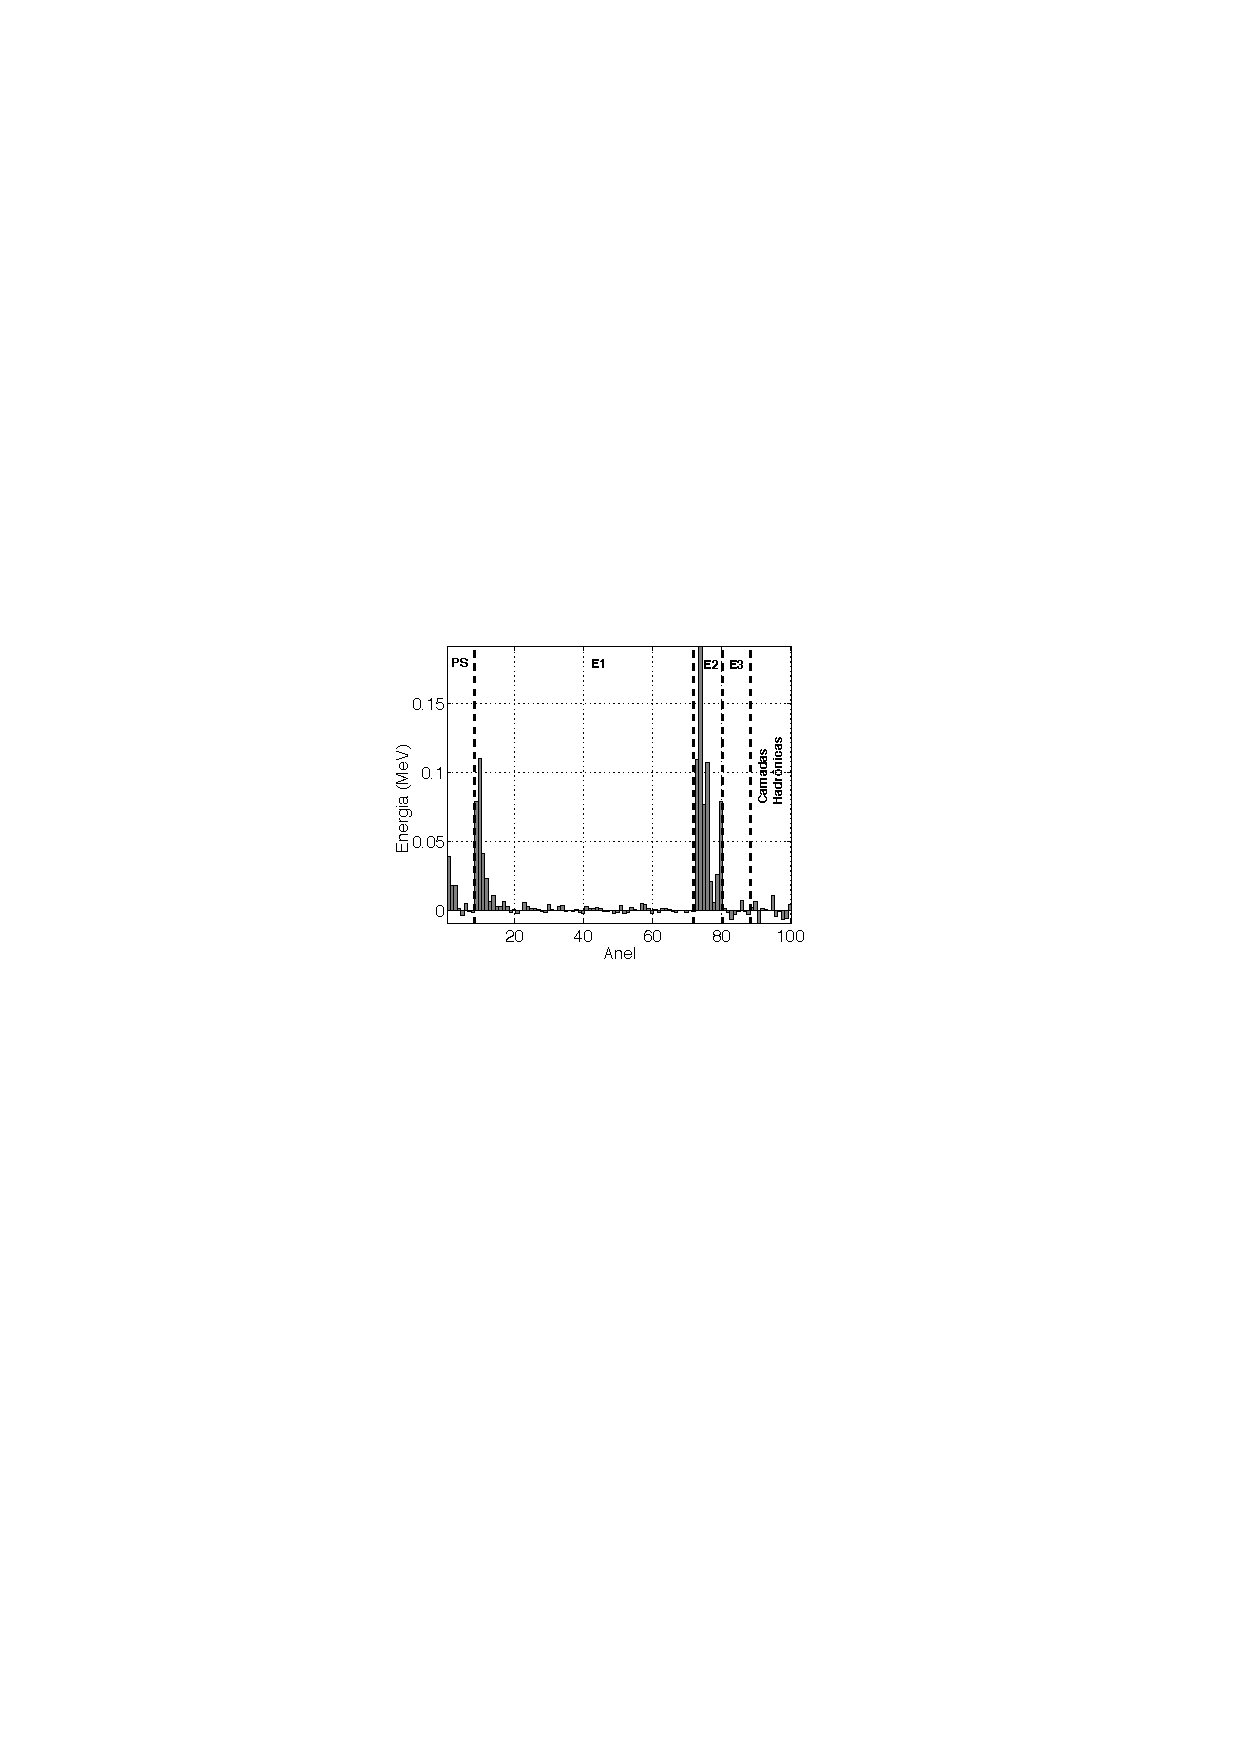
\includegraphics[width=0.45\textwidth]{imagens/perfil_aneis_jato_confundidor.pdf}
  }\\
\caption[Perfil típico para os 100 anéis de elétrons e jatos.]{Perfil típico
para os 100 anéis de elétrons (\ref{fig:perfil_aneis_eletron}) e
jatos (\ref{fig:perfil_aneis_jato}). Jatos atípicos (\ref{fig:perfil_aneis_jato_conf}) 
dificultam o processo de discriminação. A escala de energia está normalizada
pela Norma 1. Extraído de \cite{tese_eduardo}.}
\end{figure}



\subsubsection{Normalização}
\label{sssec:preproc_norm}

Neste tópico estão as descrições das normalizações testadas para a otimização do
\gls{hltringer}. Foram utilizadas normalizações presentes na literatura
utilizando tratamento estatístico dos dados, como a Esferização, MinMax, 
adicionadas de normalizações que fazem mão do conhecimento da topologia dos calorímetros, 
sua segmentação longitudinal e das diferenças entre os chuveiros \gls{em} e \gls{had}, 
buscando realçar suas características, citando entre elas a normalização
sequencial.

\newacronym[type=Abrev]{mod}{MOD}{Modificado}
\newacronym[type=Simb,\glslongpluralkey={anéis},\glsshortpluralkey={\ensuremath{r}}]
{anel}{\ensuremath{r}}{anel}

\paragraph{Energia Total (Norma 1)}
\label{par:norm_norm1}

Neste modo de normalização, cada um dos \glspl{anel} produzidos são normalizados pela energia total 
(considerando-se todas as camadas) contida em uma região de $0,4 \times 0,4$ em 
$\eta \times \phi$ do evento, fazendo-se:

\begin{equation}
r_{i}' = \frac{r_i}{\overset{N}{\underset{j=1}{\sum}} r_j}~~\forall~~i=1,2,3,...,N
\end{equation}

\noindent onde $N$ é o número de anéis produzidos, considerando todas as camadas (i.e. 100). 
O objetivo desta normalização é reduzir a influência da energia de cada evento nas análises, 
mantendo, ainda assim, a proporção de energia contida em cada anel.

%\paragraph{Fixa Seção}
%
%Neste modo de normalização, os \glslink{anel}{anéis ($r_s$)} produzidos na
%c-ésima camada
%(\gls{ps}, \gls{e1}, \gls{h1}, etc.) são normalizados pela sua média $\bar{r_s}$
%somada de
%um desvio padrão $\sigma{r_s}$, fazendo-se
%
%\begin{equation}
%r_{s}' =   \frac{r_s) }{\bar{r_s} + \sigma{r_s}} ~~\forall~~i=1,2,3,...,N_s
%\end{equation}
%
%\paragraph{Fixa Camada}
%
%Neste modo de normalização, os \glslink{anel}{anéis ($r_c$)} produzidos na
%c-ésima camada
%(\gls{ps}, \gls{e1}, \gls{h1}, etc.) são normalizados pela sua média $\bar{r_c}$
%somada de
%um desvio padrão $\sigma{r_c}$, fazendo-se
%
%\begin{equation}
%r_{c}' =   \frac{r_c) }{\bar{r_c} + \sigma{r_c}} ~~\forall~~i=1,2,3,...,N_c
%\end{equation}



\paragraph{Norma 2}
\label{par:norm2}

Cada anel foi normalizado por

\begin{equation}
r_{i}' = \frac{r_i}{||\mathbf{r}||}~~\forall~~i=1,2,3,...,N
\end{equation}

\noindent onde $||\mathbf{r}||$ é a norma 2 dos N anéis produzidos.

\paragraph{Norma 2 Camada}
\label{par:norm_camada}

Cada anel foi normalizado por

\begin{equation}
r_{c_i}' = \frac{r_{c_i}}{||\mathbf{r_c}||}~~\forall~~i=1,2,3,...,N_c
\end{equation}

\noindent onde $||\mathbf{r}||$ é a norma 2 dos $N_c$ anéis produzidos para a
c-ésima camada.

\paragraph{Norma 2 Seção}
\label{par:norm_secao}

Cada anel foi normalizado por

\begin{equation}
r_{s_{i}}' = \frac{r_{s_{i}}}{\underset{j=1}{\overset{N_s}{ \sum}} r_{s_{j}}}~~\forall~~i=1,2,3,...,N_s
\end{equation}

\noindent onde $||\mathbf{r}||$ é a norma 2 dos $N_c$ anéis produzidos para a
c-ésima camada.

\paragraph{Sequencial}
\label{par:norm_seq}

Esta técnica de normalização visa amplificar as diferenças no perfil lateral dos chuveiros produzidos. 
Nesta técnica, os anéis ($r_c$) produzidos na c-ésima camada são normalizados fazendo-se

\begin{equation}
\label{eq:normalizacao_sequencial}
r_{c_{i}}' = \frac{r_{c_{i}}}{ E_{tot_{c}} - \underset{j=1}{\overset{i-1}{\sum}} r_{c_{j}} }
\end{equation}

\noindent onde $E_{tot_{c}}$ é a energia total da c-ésima camada. Esta normalização pode ser interpretada 
como uma otimização da normalização por energia, amplificando a contribuição dos anéis mais 
externos ao centro da \gls{roi}, através da aplicação de fatores de normalização sucessivamente menores. Para 
evitar a amplificação de anéis contendo apenas ruído, quando o fator de normalização fica menor do que 
um dado limiar  ($E_{stop} = 100$~MeV), todos os anéis restantes passam a ser normalizados pela energia 
total da camada ($E_{tot_{c}}$). Adicionalmente, para evitar que camadas contendo apenas ruído sejam 
normalizadas, caso $E_{tot_{c}}$ fique abaixo de um dado limiar ($E_{thres} = 0,01$~MeV), nenhuma 
normalização é aplicada para a camada em questão.

\paragraph{Fixa}

Após obter a média dos anéis $\bar{r}$ e o seu desvio padrão $\sigma_{r}$,
aplica-se a normalização fixa através de:

\begin{equation}
r =   \frac{r}{\bar{r} + \sigma_{r}} 
\end{equation}


\paragraph{Fixa Seção}

Após obter a média dos anéis para as seções \gls{em} e \gls{had} do Sistema de
Calorímetria, $\bar{r_{EM}}$ e $\bar{r_{HAD}}$ e o seus desvios padrões
$\sigma_{r_{EM}}$ e $\sigma_{r_{HAD}}$, aplica-se a normalização fixa por seção
através de:

\begin{equation}
r_{EM}' =   \frac{r_{EM}}{\bar{r}_{EM} + \sigma_{r_{EM}}} 
\end{equation}
\begin{equation}
r_{HAD}' =   \frac{r_{HAD}}{\bar{r}_{HAD} + \sigma_{r_{HAD}}}
\end{equation}

\paragraph{Fixa Camada}

Após obter a média dos anéis para a c-ésima camada do detector (\gls{ps},
\gls{e1}, \gls{e2}, \gls{e3}, \gls{h0}, \gls{h1}, \gls{h2}), $\bar{r_c}$ e seus
desvios padrões $\sigma_{r_c}$, aplica-se a normalização fixa por camada
através de:

\begin{equation}
r_{c}' =   \frac{r_c}{\bar{r_c} + \sigma_{r_c}} ~~\forall~~i=1,2,3,...,N_c
\end{equation}

\paragraph{Mínimo e Máximo Unitários}

Cada anel foi normalizado por

\begin{equation}
r_{i}' =   \frac{r_i - \min(r_{i}) }{\max(r_{i}) - \min(r_{i})}   ~~\forall~~i=1,2,3,...,N
\end{equation}

\noindent onde $\min(r_{i})$ e $\max_{r_i}$ são, respectivamente, o valor máximo
e o valor mínimo do i-ésimo anel. Com essa normalização cada anel terá uma
distribuição contida dentro do intervalo [-1,+1].

\paragraph{Esferização dos Anéis}

Cada anel foi normalizado por

\begin{equation}
r_{i}' = \frac{r_i - \bar{r_i}}{\sigma_{r_i }}~~\forall~~i=1,2,3,...,N
\end{equation}

\noindent onde $\bar{r_i}$ e $\sigma_{r_i }$ são, respectivamente, a média e o desvio 
padrão do i-ésimo anel. 

\paragraph{Normalização Modificada}
\glsunset{mod}

Essa normalização pode ser aplicada em outras normalizações, afetando a
normalização da seção \gls{had}. Nessa região do detector, ao invés da aplicação
do método utilizado pela normalização sendo modificada, se irá alter o nível de energia 
contido nos anéis da escala de MeV para GeV, dividindo os anéis por 1000:

\begin{equation}
r_{HAD}' =   \frac{r_{HAD}}{1000}
\end{equation}



\subsubsection{Classificadores Neurais}
\label{sssec:rna}

Após a extração e normalização dos anéis pode-se utilizar uma abordagem não-segmentada, 
na qual a informação contendo as características discriminantes é concatenada em um vetor 
e então propagada para uma única \gls{rna} discriminadora, ou então uma abordagem segmentada, 
onde cada a informação normalizada da camada longitudinal do Sistema de Calorimetria é 
propagada para sua \gls{rna} específica e então combinadas em um novo
discriminador para compor a decisão. As abordagens estão esboçadas na
Figura~\ref{fig:tipo_class}. No trabalho atual foi apenas utilizada a abordagem 
não-segmentada.

\begin{figure}[ht!]
\label{fig:tipo_class}
\centering
\subfigure[]{
    \label{fig:class_nseg}
    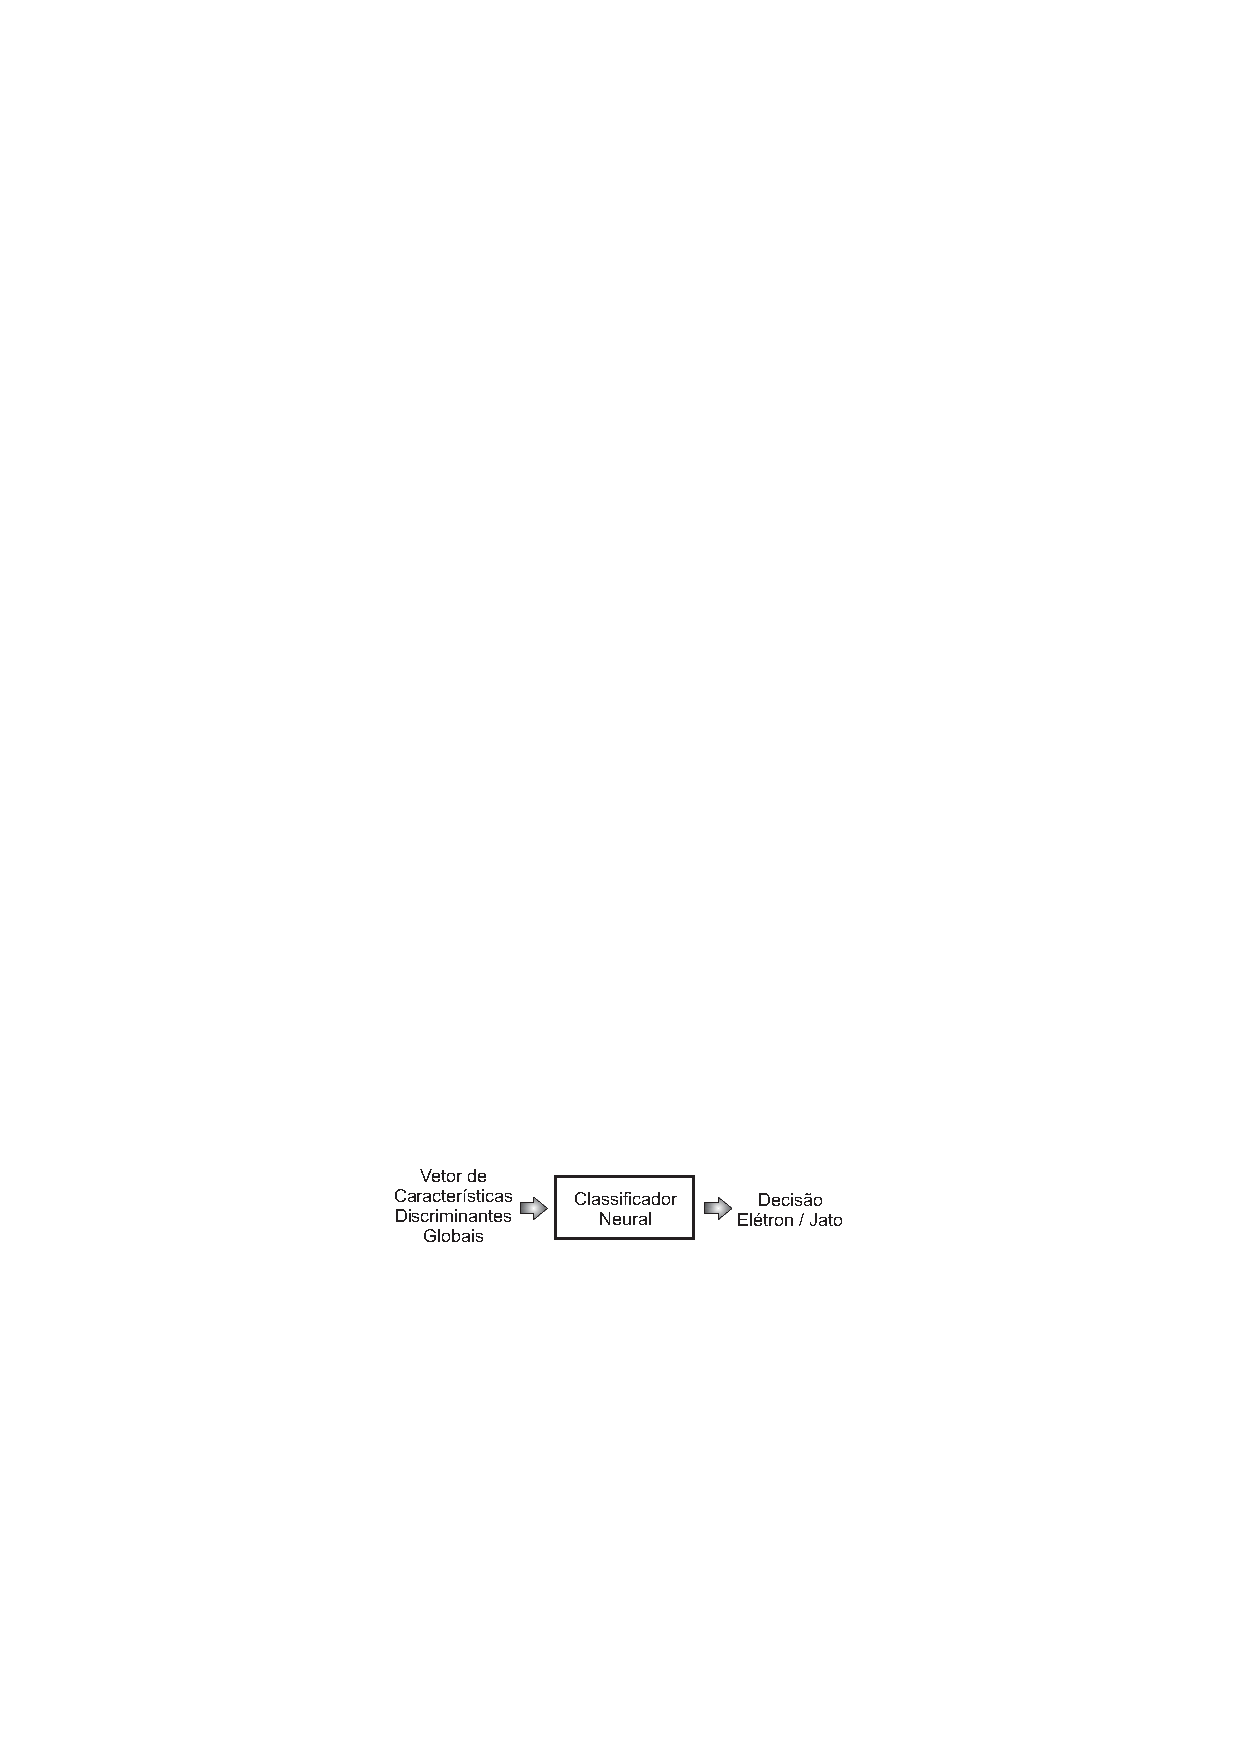
\includegraphics[width=0.5\textwidth]{imagens/classificacao_nao_segmentada.pdf}
}\\
\subfigure[]{%
    \label{fig:class_seg}
    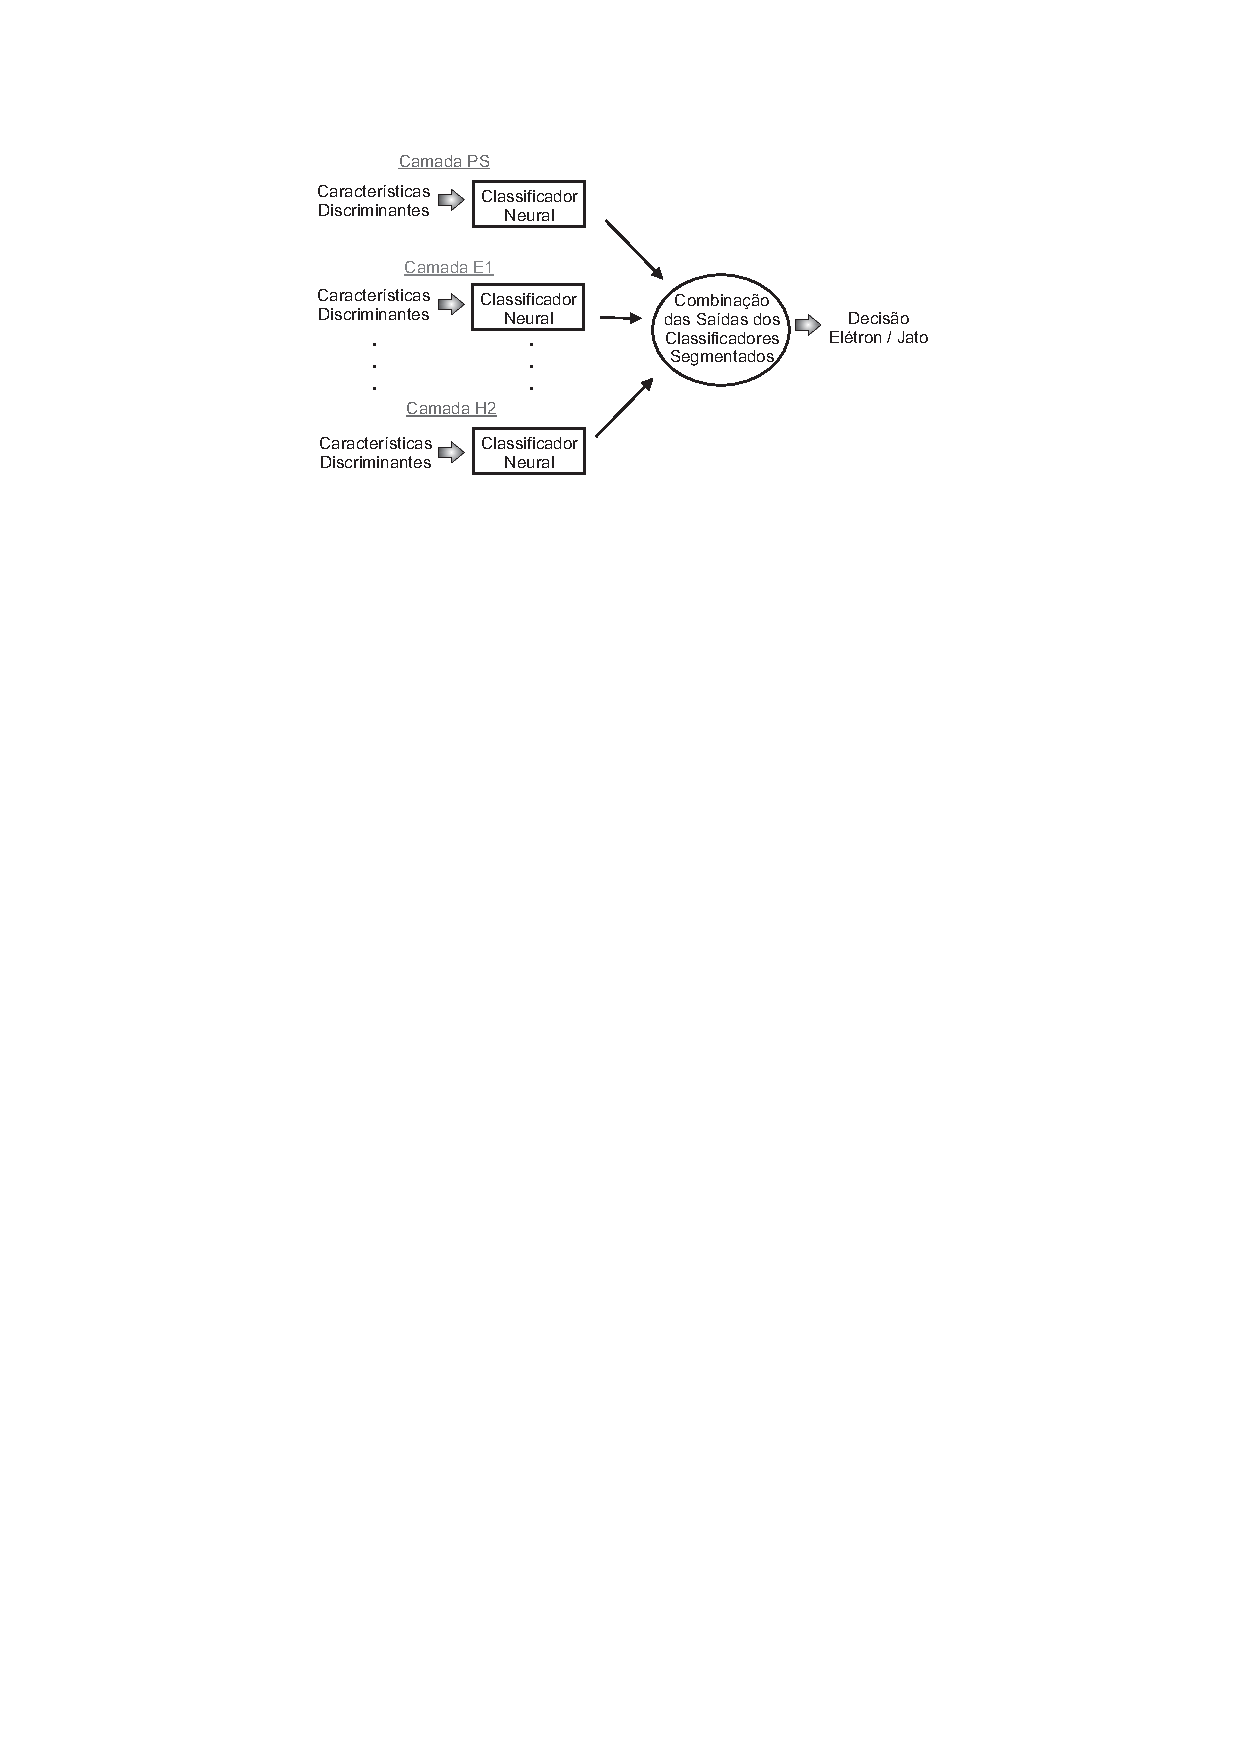
\includegraphics[width=0.7\textwidth]{imagens/classificacao_segmentada.pdf}
}
\caption[Abordagens de Discriminação: segmentada e não-segmentada.]
{Abordagem de discriminação não-segmentada
em~\ref{fig:class_nseg}, e segmentada em~\ref{fig:class_seg}. Extraído de 
\cite{tese_eduardo}.}
\end{figure}

\newacronym[type=Abrev]{rprop}{RPROP}{\emph{Resilient Back-propagation}}
\newacronym[type=Abrev]{mlp}{MLP}{\emph{Perceptron} Multicamadas}
\newacronym[type=Abrev]{mse}{MSE}{Erro Quadrático Médio}

A topologia de uma \gls{rna} composta de uma rede \gls{mlp} alimentada em
cascata, ou \emph{feed-forward}, com uma camada escondida está esboçada na
Figura~\ref{fig:topologia_rna}. Estão simbolizados três neurônios de saída, para
o caso de separação em três classes, mas a rede utilizada tem apenas uma saída,
suficiente para realizar a discriminação em duas classes, as partículas \gls{em}
compondo o sinal: elétrons, pósitrons e fótons; e o ruído físico: os
hádrons dos jatos hadrônicos. Os alvos utilizados para as classes foi de +1 para o
conjunto de sinal, e -1 para o conjunto de ruído físico.
A camada de entrada recebe o vetor de dados, com os 100 anéis normalizados, enquanto o número de 
neurônios na camada escondida varia conforme a representação dos dados, 
sendo determinado através de um estudo de exaustão. Todos os neurônios utilizam
função de ativação tipo tangente hiperbólica.

\begin{figure}[ht!]
\label{fig:topologia_rna}
\centering
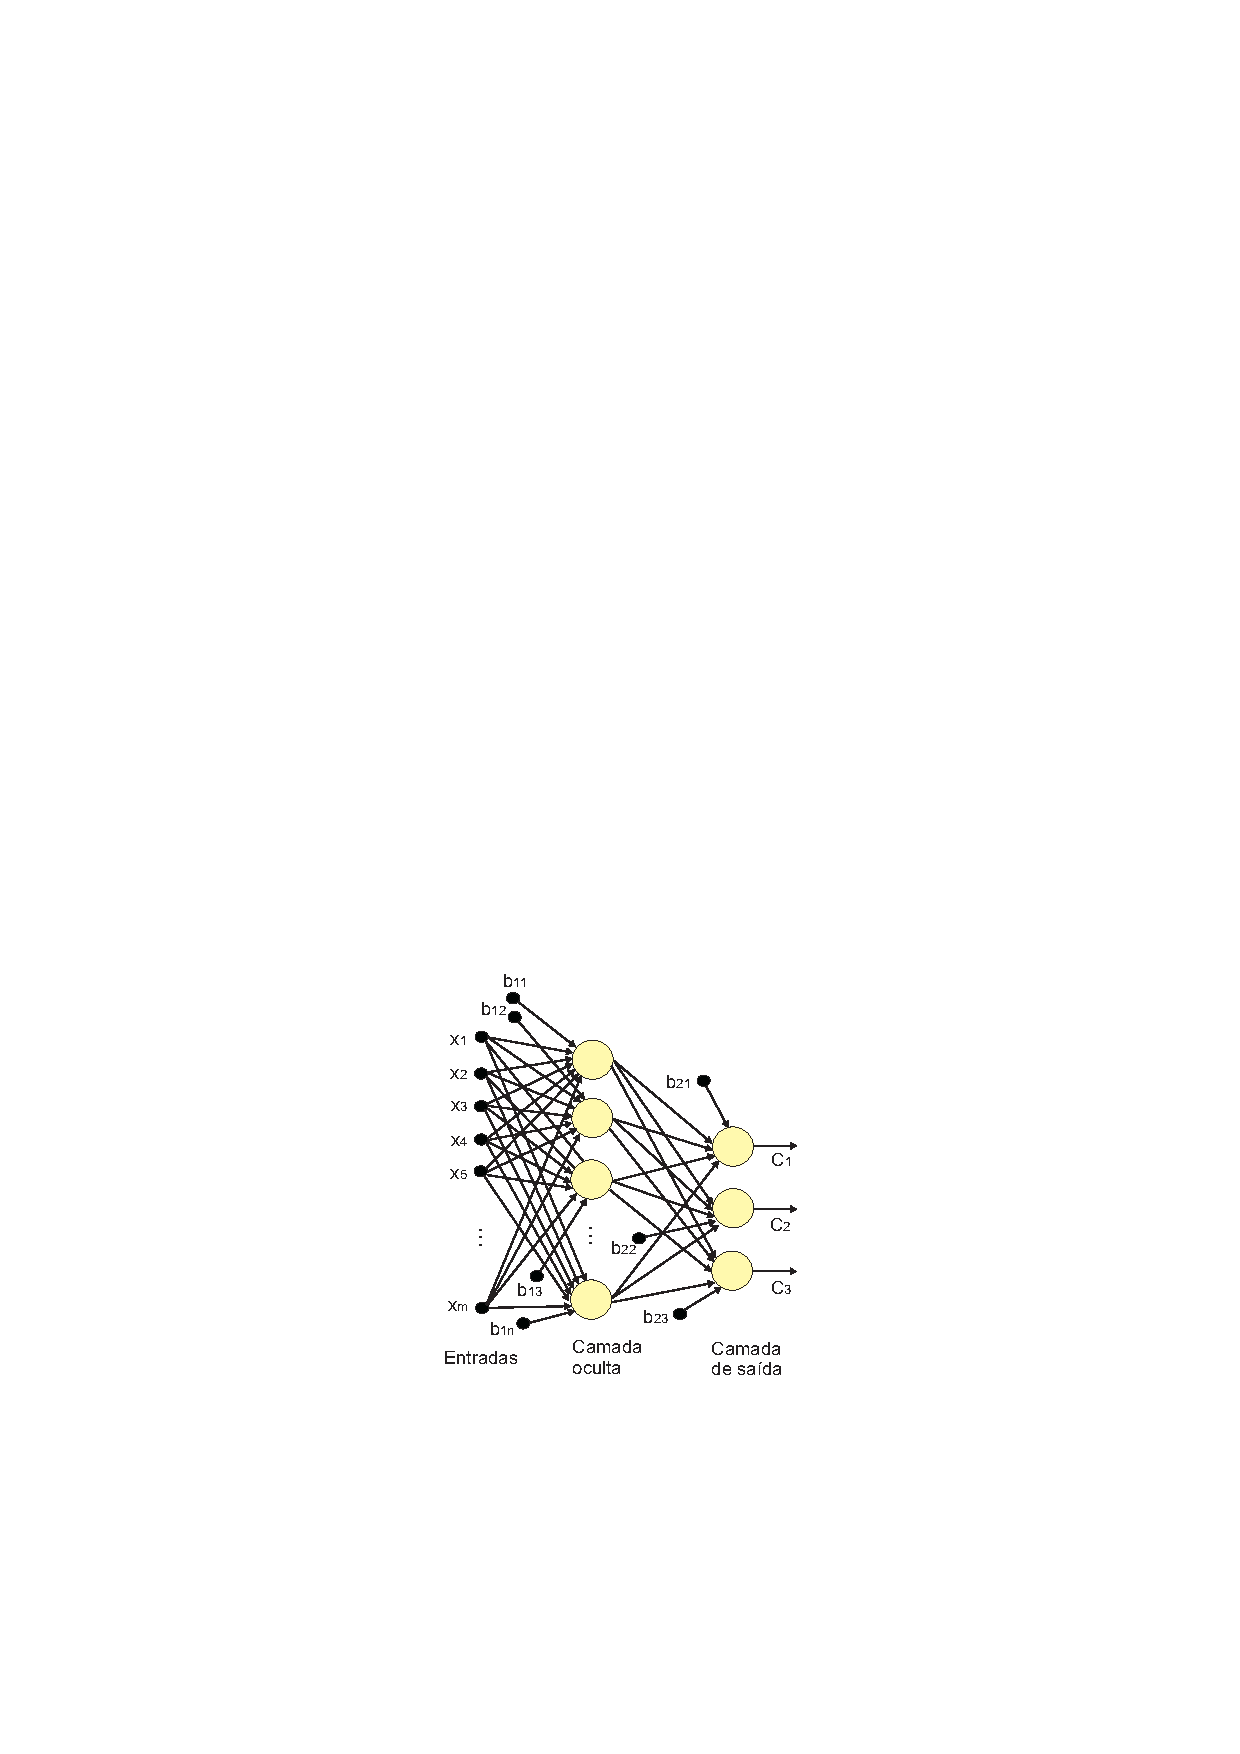
\includegraphics[width=0.4\textwidth]{imagens/topologia_rna.pdf}
\caption[Topologia de uma MLP alimentada em cascata.]{Topologia de uma
MLP alimentada em cascata. Extraído de \cite{tese_eduardo}.}
\end{figure}

É necessário realizar o treinamento das \glspl{rna} para que as mesmas possam, de
fato, reconhecer padrões. Para o processo de treinamento se
utilizou, na inicialização dos pesos, o algoritmo de \emph{Nguyen-Widrow} \cite{initnw}, 
enquanto no treinamento o \gls{rprop} \cite{rprop}, devido a sua simplicidade de uso e 
rápida convergência. Para realizar o treinamento secciona-se o conjunto de dados
em três partes: 

\newacronym[type=Abrev]{det}{\ensuremath{\text{DET}}}{Taxa de Detecção}
\newacronym[type=Abrev]{deteg}{\ensuremath{\text{DET}_{e/\gamma}}}{Taxa de Detecção de elétrons,
pósitrons e fótons}
\newacronym[type=Abrev]{detj}{\ensuremath{\text{DET}_{j}}}{Taxa de Detecção de hádrons}
\newacronym[type=Abrev]{fa}{\ensuremath{\text{FA}}}{Taxa de Falso Alarme}

\newacronym[type=Abrev]{trn}{TRN}{Conjunto de Treino}
\newacronym[type=Abrev]{val}{VAL}{Conjunto de Validação}
\newacronym[type=Abrev]{tst}{TST}{Conjunto de Teste}

\begin{itemize} 
\item \textbf{\gls{trn}} (neste estudo totalizando 50\% dos dados em
casos de pouca estatística e 33\% no oposto): 
no qual se será atualizado os pesos sinápticos da \gls{rna} de modo a minimizar uma função 
custo, na qual a utilizada foi o \gls{mse};
\item \textbf{\gls{val}} (16,6\%/33,3\%): utilizado para garantir a boa 
generalização da \gls{rna}; 
\item \textbf{\gls{tst}} (33,3\% para ambos os casos): 
estatística não observada pela \gls{rna} durante seu treinamento, utilizada para 
testar sua performance. 
\end{itemize}

Para a análise de eficiência de discriminação, alguns parâmetros precisam ser definidos:

\begin{itemize}
\item \textbf{\gls{det}}: taxa de uma classe corretamente identificada pelo
discriminador. Geralmente se refere a taxa de sinal, no caso do Canal~\gls{eg} a
\gls{deteg}, mas também podendo ser utilizada para o caso de ruído, \gls{detj}.
Caso não identificado a classe de detecção, então se estará referindo a
\gls{deteg};
\item \textbf{\gls{fa}}: taxa da classe constituinte de ruído erroneamente
identificada pelo discriminador. No Canal~\gls{eg} a taxa de hádrons que formam os
jatos hadrônicos identificados como \gls{eg}. Também pode
ser obtida como: $1-\gls{detj}$.
\end{itemize}

\newacronym[type=Abrev]{sp}{SP}{Produto Soma-Produto}

Dois critérios podem ser utilizados para medir a figura de mérito da \gls{rna}
durante o treinamento, aplicando-se aos conjuntos de validação e teste: \gls{mse} 
e \gls{sp}. O \gls{mse} visa encontrar o ponto onde as saídas da \gls{rna} ficam
o mais próximo possível do alvo especificado. O \gls{sp} é relacionado por:

\begin{equation} \label{eq:produto_sp}
SP = \sqrt{ \sqrt{\gls{deteg}\times \gls{detj}}\times\frac{\gls{deteg}+\gls{detj}}{2}}\times100\%
\end{equation}

\noindent no caso de discriminação binária. Esse critério visa indicar ao
processo de treinamento o ponto onde a distinção máxima entre classes é obtido,
sendo o critério mais apropriado para \glspl{rna} destinadas ao reconhecimento de
padrões \cite{tese_torres}.

O número de épocas (ou iterações) de treinamento foi ilimitado, de forma que o
critério de parada para o processo de treinamento utilizado é de 50 falhas na tentativa
de melhora da figura de mérito para a validação. 
Utilizou-se o critério \emph{Save the Best}, onde os pesos sinápticos na época com 
o melhor resultado da figura de mérito para o conjunto de teste são armazenados 
para a utilização da rede. Foi utilizado o critério de batelada, onde se sorteia os
dados a se realizarem o treinamento, com o tamanho do menor 
conjunto de dados de treinamento, geralmente sendo esse o de elétrons, para
evitar uma maior estatística de um dos conjuntos durante o treinamento. O
processo de treinamento é repetido $N$ vezes para evitar-se flutuação
estatística, inicializando novos pesos aleatórios para cada configuração 
testada.

\newacronym[type=Abrev]{roc}{ROC}{Região de Critério}

Após o treinamento é possível especificar a \gls{det} (no caso de partículas \gls{eg}) 
e \gls{fa} através da escolha do limiar de decisão, aonde valores maiores ao limiar serão considerados
como \gls{eg} e os menores jatos. A escolha do limiar tem o seu compromisso
representados nas curvas \gls{roc}: quanto maior a \gls{det}, também será a
\gls{fa}. O \gls{sp} tenta conciliar o compromisso entre a detecção de
partículas \gls{eg} e jatos, o que não é desejado quando no \gls{sf}, onde se
deseja apenas filtrar os eventos a capacidade de armazenamento e processamento a
posteriori, evitando a perda prematura dos dados. Assim, o \gls{sp} é utilizado
apenas como figura de mérito para o treinamento das redes, e não como critério
de seleção para o limiar de decisão, que visa buscar a melhor \gls{det} sem
comprometer a capacidade de armazenamento e processamento a posteriori.

\section{O Sistema de Reconstrução (SR)}
\label{sec:sr}

O papel da reconstrução de física \cite{physics_perf_expected,atlas_computing_tdr}, 
realizada pelo \gls{sr}, é de derivar dos dados armazenados os parâmetros das partículas 
e auxiliar na informação necessária para a análise de física. 
Cada subdetector do \gls{atlas} utiliza um método individual de calibração de
sua informação, por exemplo, os calorímetros realizam a calibração da energias no
nível das suas células, e a informação armazenada pelos especialistas do
calorímetro para uma dada temporada é utilizada para evitar as células ruidosas ou mortas. 
Posteriormente cada canal de física utiliza a informação contida nos
subdetectores de modo a identificar as partículas de interesse e seus
parâmetros, realizando outras calibrações para garantir a melhor precisão
possível nesses parâmetros, de forma a facilitar e melhorar a qualidade de
descobertas, como a do bóssom de Higgs, entendimento de física ainda não bem
conhecida, como o quark \emph{top}, e outros objetivos citados em
\ref{ssec:obj_lhc}.

Muitas semelhanças podem ser observadas nos algoritmos do \gls{hlt}, em especial o
\gls{ef}, com o \gls{sr}. Na verdade, os algoritmos do \gls{sf} foram feitos
baseados no \gls{sr} com o objetivo de evitar ao máximo a polarização dos dados
armazenados. As diferenças entre os dois ambientes, como já foi dito, está na
maior restrição de tempo e robustez dos algoritmos no ambiente do \gls{sf}, de
forma que os algoritmos no \gls{sf} realizam análises menos refinadas. Por esse
motivo, os cortes utilizados no \gls{sf} são relaxados quando em comparação com
os do \gls{sr} para evitar a perda prematura de física de partículas em que não
se há muita certeza do que ocorreu. Nesses casos, prefere-se armazenar os
dados para o \gls{sf} analisar os eventos com mais detalhes e tomar uma decisão
com maior precisão, desde que isso não ultrapasse os recursos computacionais para 
armazenamento e processamento dos dados.

\subsection{\texorpdfstring{Algoritmo $e/\gamma$ Padrão}{Algoritmo eGamma Padrão}}
\label{ssec:egamma}

O algoritmo padrão de reconstrução de física a posteriori não é muito distinto
daquele descrito para o \gls{ef} da cadeia \gls{eg} no Tópico~\ref{ssec:cadeia_egamma},
inclusive já sendo realizadas algumas distinções entre os algoritmos que serão
aqui complementadas.

Primeiro, precisa-se ter em mente que o algoritmo a posteriori utiliza
parâmetros com maiores precisões. Calibrações, como a posição de \gls{eta}, e 
da energia depositada em cada camada é realizada com maior precisão. Outras
calibrações, como a posição em \gls{phi} e calibrações no nível de células,
também são realizadas no \gls{sr}, o que não ocorre para o \gls{hlt}.

Para a construção dos aglomerados de células no calorímetro se utiliza um algoritmo 
de janela deslizante \cite{sliding_window}.
Dois tipos de aglomerados podem ser construídos: os aglomerados \gls{em}, no caso de elétrons e fótons; 
e os combinados, na busca de jatos e identificação de
táons-léptons. São utilizados três passos no algoritmo, a construção das torres de
células, a procura por uma semente e o preenchimento do aglomerado, onde esses dois
últimos passos ocorrem juntos para os aglomerados combinados. 

Serão abordados apenas os aglomerados \gls{em}, uma vez apenas eles são
utilizados pelo Canal~\gls{eg}. O processo de construção é realizado apenas para 
$|\gls{eta}|<2,5$, onde é realizado a construção das torres, o Sistema de Calorimetria é 
dividido em uma grade de $0,025\times0,025$, através da soma da energia das
células das camadas longitudinais do \gls{ecal} contidas dentro da
região. Em seguida, uma janela de $5\times5$ torres
procura por uma região que ultrapasse um limiar para $\gls{Et} > 2,5$ GeV e 
que seja um máximo local (a ideia de máximo local é a mesma que àquela citada
para o \gls{l1}, presente no tópico já referenciado). Quando encontrado, é gerada uma
semente cuja posição é calculada através da ponderação de energia das células contidas 
em uma janela concêntrica a anterior mas menor ($3\times3$ torres) para evitar o
acumulo de ruído, com as posições das células.
Para remover duplicatas, ao se ocorrer múltiplas sementes dentro de uma região
$2\times2$ torres, apenas a semente mais energética será armazenada. Os
aglomerados são reconstruídos com seus tamanhos 
específicos dependente da partícula e sua incidência ($3\times7$ para elétrons e fótons convertidos,
$3\times5$ para fótons não-convertidos quando incidindo no barril, e $5\times5$ na
tampa). O processo se inicia na \gls{e2} através da construção do
aglomerado a partir da posição da semente. Então o baricentro de energia é
calculado e propagado para a \gls{e1} e \gls{e3}, aonde são gerados os
aglomerados para essas camadas. Para o \gls{ps} é utilizado como centro o
baricentro de energia da \gls{e1}. A partir desse aglomerado serão retiradas 
as variáveis físicas utilizadas para representar a propagação do chuveiro, que
serão utilizadas para realizar a discriminação. Essas variáveis são algumas
daquelas contidas na Tabela~\ref{tab:cortes_em}.  
Um algoritmo alternativo também pode ser utilizado para a construção
de aglomerados topológicos, onde a ideia básica é agrupar as células 
vizinhas a semente que tiverem energia significante quando comparado ao ruído
esperado.

A informação do aglomerado é combinado com a reconstrução do traço
\cite{physics_perf_expected} das partículas para fazer a separação de elétrons e fótons, assim como melhorar o
potencial de identificação de elétrons. O traço, no qual o último ponto no
\gls{trt} tiver o menor $\Delta\text{R}$ (equação~\ref{eq:dist_clust_traco}) ao baricentro da \gls{e1}, 
é utilizado para a combinação entre o traço e aglomerado. Os parâmetros do traço
e relação traço-aglomerado podem ser utilizados para gerar as outras variáveis
da Tabela~\ref{tab:cortes_em}.

Os requerimentos citados no \gls{sf} também se aplicam, sendo eles: \emph{loose}, 
\emph{medium} e \emph{tight}. Eles são utilizados para
identificar a característica da estatística utilizada para a análise.

Além do algoritmo padrão, a colaboração também realizou estudos de técnicas
multivariáveis, incluindo discriminadores de Máxima Verossimilhança, árvores 
de decisões ampliadas e redes neurais \cite{physics_perf_expected}.


\subsection{\texorpdfstring{$e/\gamma$ \emph{Calorimeter Ringer}
(EgCaloRinger)}{eGamma Calorimeter Ringer (EgCaloRinger)}}
\label{ssec:egringer}

Uma dificuldade encontrada para a introdução do \gls{hltringer} na cadeia de
filtragem \gls{eg} é sua configuração diferente ao \gls{t2calo}, causando o
receio, por parte da Colaboração, que ocorra a polarização dos dados. Por isso, foi requisitado a
implementação de uma versão do algoritmo para a análise a posteriori, permitindo
a utilização da ferramenta pela Colaboração e a confiança de que as partículas
selecionadas estão coerentes com a física. O \gls{egcaloringer} é a
implementação do algoritmo proposto para o ambiente do \gls{sf}.

Embora a estrutura do algoritmo seja a mesma que aquela explicada para o \gls{l2}, no
Tópico~\ref{ssec:hlt_ringer}, realizando a construção dos anéis, normalizando e
então propagando para uma \gls{rna}, há diferenças nas versões devido aos ambientes de implementação, 
de maneira que as duas versões não são idênticas. Primeiro, o \gls{sf} realiza a calibração da energia 
no nível das células, de forma que os anéis do \gls{egcaloringer} terão 
valores mais refinados de energia, enquanto o \gls{hltringer} utiliza o
valor cru medido pelo calorímetro. Outra mudança importante quanto a construção
dos anéis está na disponibilidade de todas as células para este, de forma que
os anéis serão completamente construídos, enquanto naquele apenas as
células disponíveis na \gls{roi} podem ser acessadas, deixando anéis em aberto. 
Finalmente, a diferença da semente utilizada para a construção dos anéis entre o \gls{sf} e \gls{l2}
também modificarão o processo de anelamento, onde o \gls{hltringer} utiliza
a célula quente da \gls{e2} contida na \gls{roi}, e sua versão a
posteriori o centro do aglomerado calculado pelo \gls{sf}, que contém uma ponderação da
distribuição de energia entre as células de todas as camadas do \gls{ecal}
contidas em uma região $3\times3$ torres (cada torre tem $0,025\times0,025$ em
$\gls{eta}\times\gls{phi}$), sendo uma posição muito mais realística 
do centro do chuveiro.


\subsubsection{Implementação}
\label{sssec:egringer_impl}

A implementação do \gls{egcaloringer} foi realizada garantindo que a operação
dos algoritmos já implementados pela Colaboração não fossem afetados, alterando
o mínimo de código necessário dos destes e garantindo a operação normal da
reconstrução do Canal~\gls{eg}. O \gls{egcaloringer} não deveria ser executado
exceto quando explicitamente exigido pelo usuário. 

Para cumprir com esse requisito se idealizou a 
estrutura disposta na Figura~\ref{fig:implementacao_ringer}, de forma que apenas
quando adicionado a configuração via \glsdesc{jo} o algoritmo é executado.
Durante a inicialização, o \emph{egammaBuilder} organiza os algoritmos no
nível de informação dos subdetectores, adicionando os algoritmos de reconstrução
de traços, vértices e aglomerados do calorímetro, e chama a configuração do
\emph{EMPIDBuilder} que irá adicionar os algoritmos para a geração das variáveis
físicas utilizadas para a discriminação. Quando exigido na \glsdesc{jo}, o
processo de construção dos anéis realizado pelo algoritmo \emph{RingerCaloTool} 
é adicionado durante a inicialização ao \emph{egammaBuilder}, 
que irá requisitar ao \emph{EMPIDBuilder} a adição da
execução do algoritmo de discriminação do \gls{egcaloringer} pelo
\emph{egammaEPiRingerCaloTool}, onde será executada a normalização especificada 
na \glsdesc{jo} e a propagação das informações contidas nos anéis normalizados 
na \gls{rna} também especificada. 

\begin{figure}[ht!]
\label{fig:implementacao_ringer}
\centering
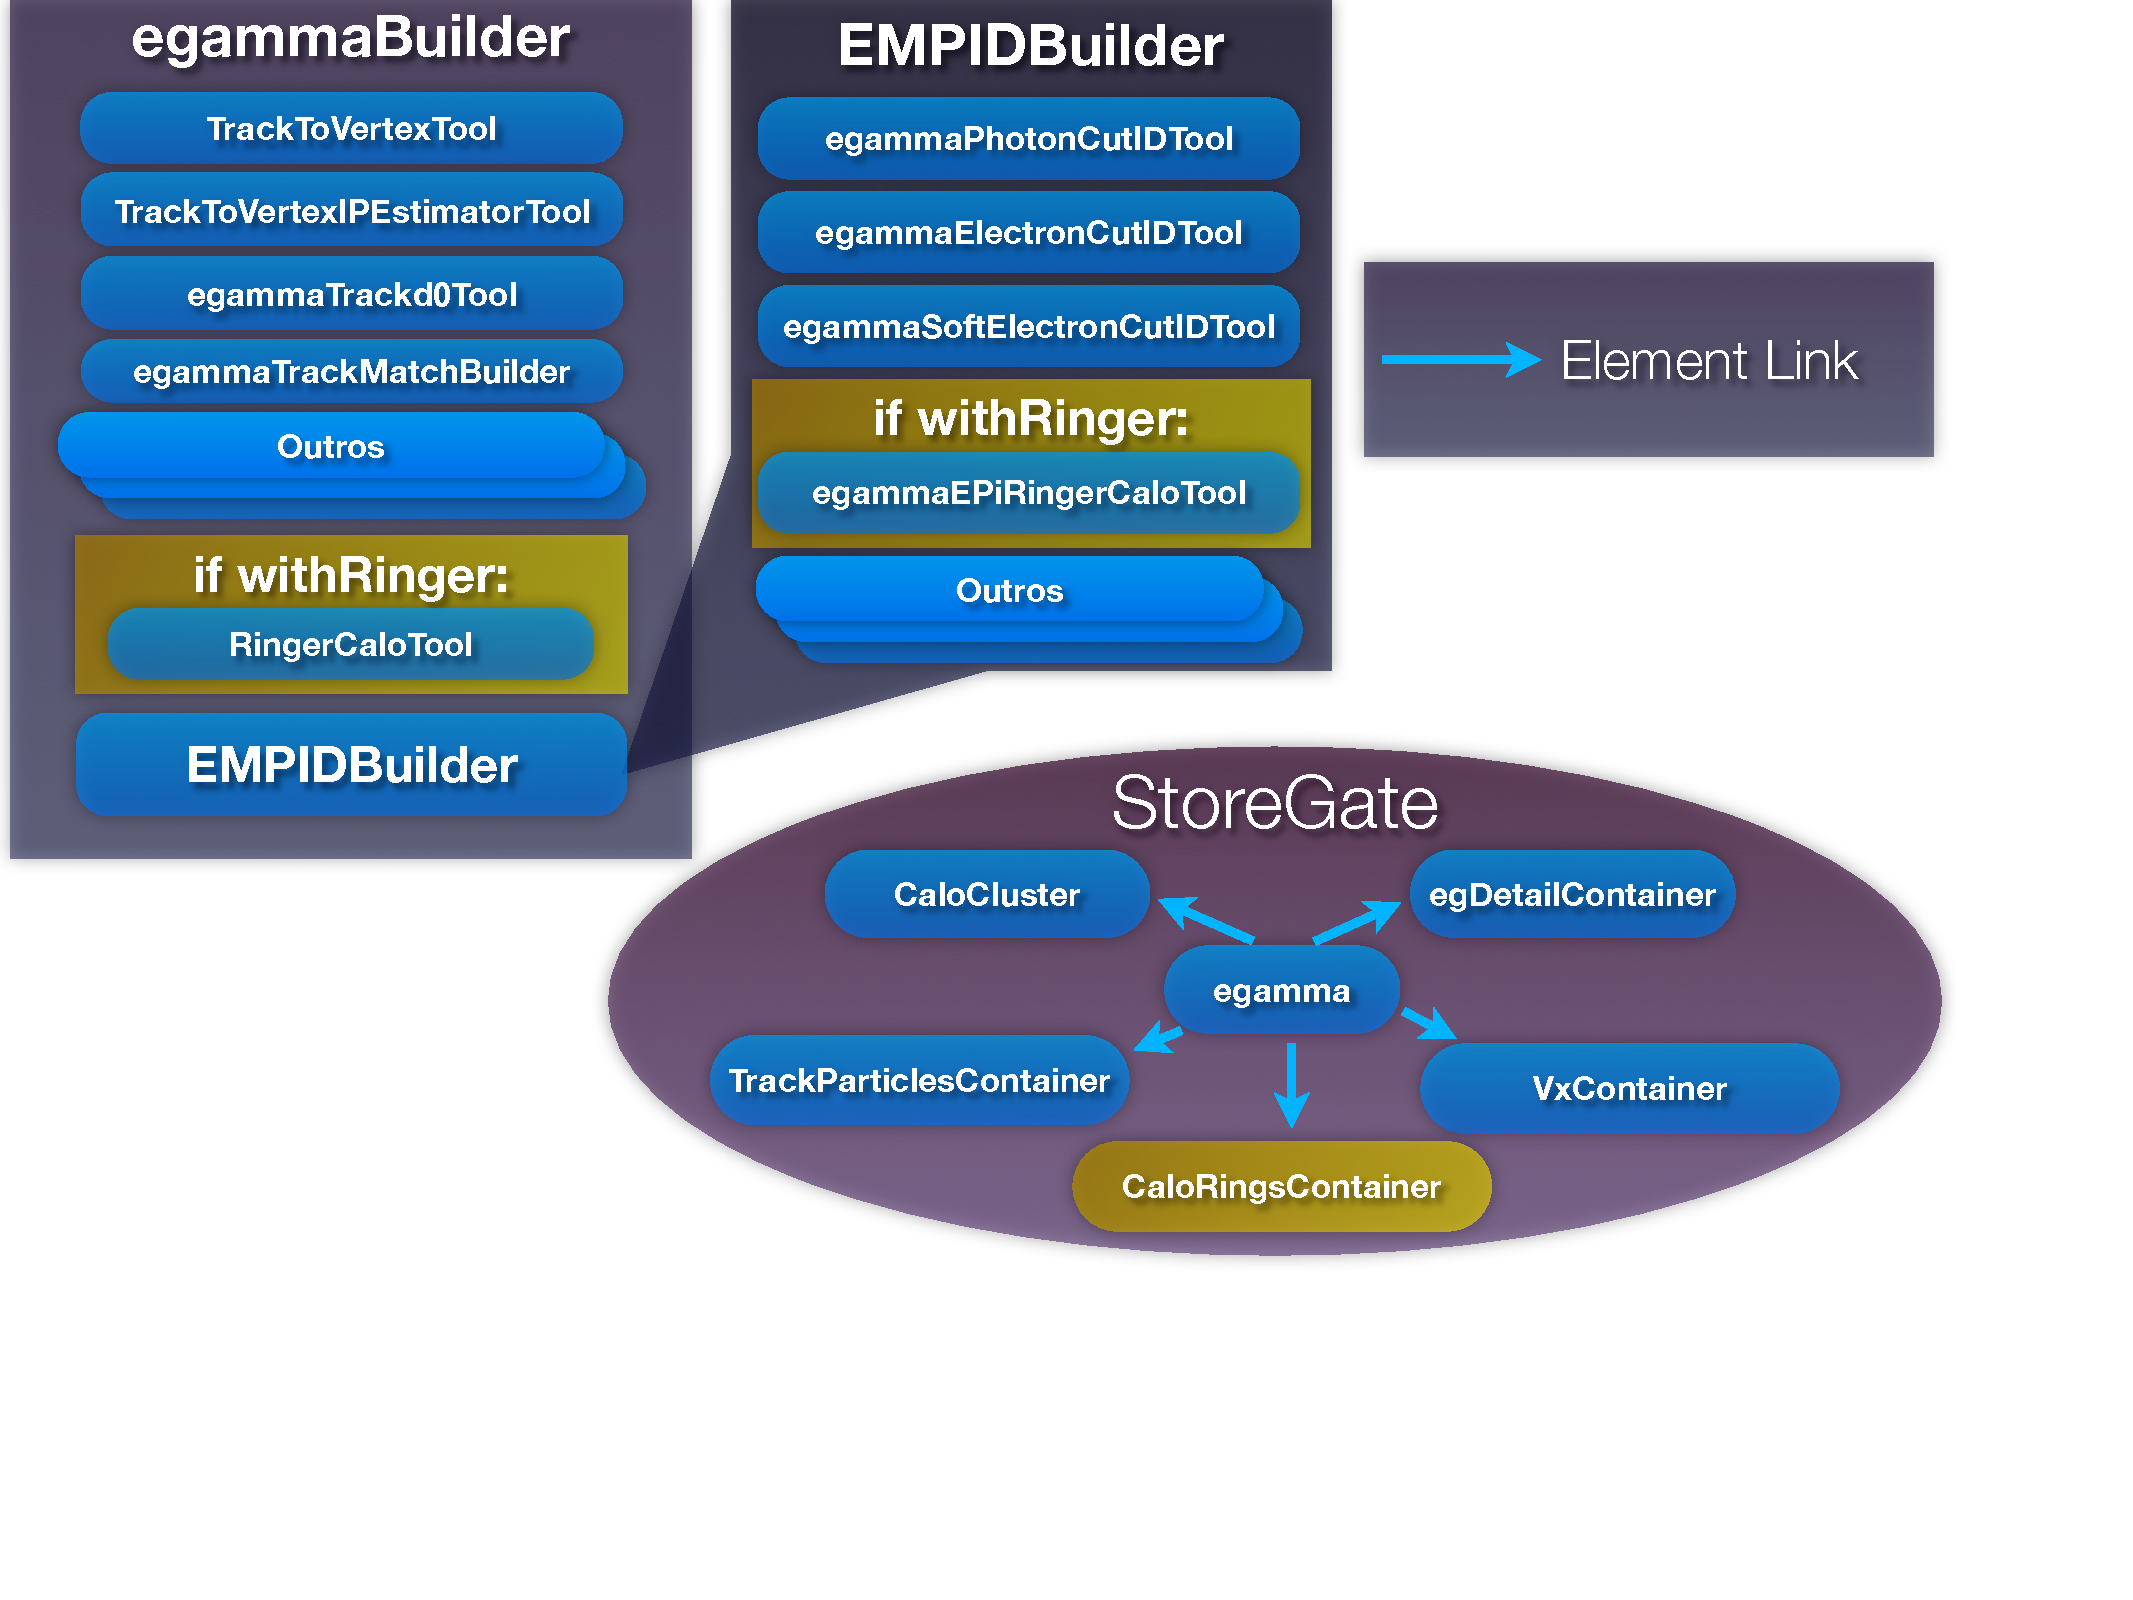
\includegraphics[width=1.0\textwidth]{imagens/implementacao_ringer.pdf}
\caption[Diagrama de implementação do \protect\gls{egcaloringer}]{Diagrama de
implementação do \gls{egcaloringer}.}
\end{figure}

Durante a execução, o \emph{egammaBuilder}
procura para cada evento os objetos de reconstrução dos subdetectores,
em busca por aglomerados e seus respectivos traços, criando um objeto 
\emph{egamma} transiente\footnote{Memória transiente é a informação contida na memória 
virtual do computador.} com as informações no \gls{sg}. A informação será
armazenada dentro recipiente \emph{egammaContainer} que irá ter \emph{Element
Links}\footnote{Pode ser interpretado com uma espécie de ponteiro de C++, embora
contenha outras informações além da posição de memória do objeto.} para o seu
respectivo aglomerado de células (\emph{CaloCluster}), traço
(\emph{TrackParticlesContainer}), vértice (\emph{VxContainer}), e detalhes como
propriedades do chuveiro, reconstrução do \emph{bremsstrahlung}, etc. (\emph{egDetailContainer}). 
O objeto \emph{egamma} é rotulado como um candidato a elétron, fóton, ou 
fóton convertido dependendo dessas informações. Se o \emph{RingerCaloTool}
estiver habilitado, durante a geração dos candidatos também será executado o
processo de geração dos anéis, que serão armazenados de modo transitório no
recipiente \emph{CaloRingsContainer}, também ligado ao seu objeto \emph{egamma}
através do elo gerado pelo \emph{Element Link}. Após o preenchimento do
\emph{egamma} com as informações do detector, o \emph{egammaBuilder} chama a
execução do algoritmo \emph{EMPIDBuilder}, onde serão geradas as variáveis 
físicas do algoritmo padrão, que serão armazenadas no \gls{sg} dentro do
\emph{egamma} através do objeto \emph{egPID}. Novamente se habilitado, após a
execução do algoritmo padrão, será realizada a execução do
\emph{egammaEPiRingerCaloTool}, que também irá armazenar a sua resposta no
\emph{egPID}.

As variáveis são então tornadas persistentes\footnote{Memória persistente é a informação
contida em disco rígido.}, onde os anéis e a saída neural só serão armazenados
se o \gls{egcaloringer} tiver sido habilitado. Na primeira implementação
realizada em Março de 2011, apenas a transformação em memória persistente 
no nível de \gls{aod} não foi implementada. A análise em \glspl{esd} 
só pode ser realizada por \gls{ara},
sendo um processo relativamente complexo.
A compatibilidade com dados mais simples de análise foi realizada, como a
\gls{cbnta} e \emph{TrigEgammaNtuple}, um arquivo de análise especial gerado
pelo grupo \gls{hlt} do Canal~\gls{eg}. Essa versão está disponível a partir da
distribuição \emph{AtlasOffline-17-00-00} do \emph{Athena}.

Um segundo passo de implementação foi realizada em Agosto adicionando a
compatibilidade do algoritmo para \gls{d3pd} e \gls{aod}, mas ainda não foi
adicionado ao código oficial da Colaboração.




\chapter{Resultados e Discussão}
\label{cap:resultados}

Este capítulo é dedicado à apresentação dos resultados e a discussão dos estudos
realizados. A primeira abordagem (Seção~\ref{sec:norm}) tratou a otimização do
algoritmo através da normalização mais indicada para o \gls{hltringer}, 
a versão do algoritmo proposto no \glsdesc{l2}, que teve os resultados 
posteriormente confirmados nos estudos realizados
por \cite{tese_torres}. Em seguida, serão apresentados os resultados para a
versão do algoritmo no \gls{sr} (Seção~\ref{sec:efic_egcalo}), o ambiente de
reconstrução da física a posteriori.


\section{Otimização do \emph{HLT\_Ringer}: Normalização}
\label{sec:norm}

Este estudo foi dedicado a escolha da normalização a ser utilizada nos
dados antes da propagação dos anéis para a \gls{rna}. Foi utilizada a
implementação do algoritmo proposto para o \gls{sf}, pois na época ainda não
havia sido requisitado pela Colaboração a implementação da versão para o \gls{sr}. Uma descrição das
normalizações testadas foi realizada no Tópico~\ref{sssec:preproc_norm}. Foram
utilizadas simulações de \gls{mc} de 2008, contendo elétrons isolados (não sendo
estudado, assim, o efeito de Empilhamento) para o conjunto de sinal e jatos com 
\gls{Et} máximo de 17 GeV para o conjunto de ruído. As redes foram treinadas com
os parâmetros especificados no Tópico~\ref{sssec:rna}, com a exceção da
utilização de apenas uma inicialização da \gls{rna}, de forma que os resultados
estavam haver flutuação estatística nos resultados indicados. Contudo, os resultados 
foram reproduzidos por \cite{tese_torres} para as normalizações que se ressaltaram 
neste estudo utilizando 10 inicializações, obtendo resultados semelhates de 
forma que a flutuação não afetou significativamente os resultados obtidos. O
estudo também considerou os dois critérios utilizados durante o treinamento da
\gls{rna} como figura de mérito, de modo a verificar se a utilização do \gls{sp}
como critério de parada ao invés do \gls{mse} realmente melhoraria a perfomance
do \gls{rna}.

\begin{table}[ht!]
\centering
\resizebox{\textwidth}{!}{
\begin{tabular}{
>{\global\let\currentrowstyle\relax}p{4.5cm}
>{\centering\arraybackslash\currentrowstyle}p{1.5cm}
>{\centering\arraybackslash\currentrowstyle}p{1.5cm}
>{\centering\arraybackslash\currentrowstyle}p{1.5cm}
>{\sl\centering\arraybackslash\currentrowstyle}p{1.5cm}
>{\centering\arraybackslash\currentrowstyle}p{1.5cm}
>{\centering\arraybackslash\currentrowstyle}p{1.5cm}
>{\centering\arraybackslash\currentrowstyle}p{1.5cm}}
\hline \hline
\textbf{Normalização}&\textbf{Épocas}&\textbf{\gls{mse}\linebreak
TRN}& \textbf{{Critério\linebreak VAL}}&\textbf{\gls{sp}\linebreak
TST}&\textbf{\gls{det}\linebreak TST}&\textbf{\gls{fa}\linebreak
TST}&\textbf{Limiar}\\
\hline \hline
Fixa \gls{sp}                   &503&0.0418&98.7320&98.7498&99.2925&1.7914&0.028\\\hline
\rowstyle{\bfseries}%
Fixa Seção \gls{sp}             &339&0.0415&98.7370&98.7544&99.3257&1.8152&-0.016\\\hline
Fixa Seção \gls{sp} \gls{mod}   &329&0.0445&98.7168&98.7349&99.2721&1.8009&0.036\\\hline
Fixa Camada \gls{sp}            &295&0.0424&98.7218&98.7309&99.2938&1.8304&-0.028\\\hline
\rowstyle{\bfseries}%
Norma 1 \gls{sp}                 &325&0.0427&98.6154&98.6087&99.2798&2.0601&-0.052\\\hline
Norma 2 \gls{sp}                 &101&0.0444&98.6357&98.6399&99.0827&1.8019&0.224\\\hline
Norma 2 Seção \gls{sp}           &477&0.0546&98.3972&98.4319&99.1426&2.2764&0.028\\\hline
Norma 2 Camada \gls{sp}          &584&0.0615&98.1071&98.0881&98.7069&2.5289&0.052\\\hline
Sequencial \gls{sp}             &837&0.0610&98.0918&98.1530&98.7242&2.4165&0.088\\\hline
MinMax \gls{sp}                 &63 &0.8899&92.7524&92.8777&94.1037&8.3404&0.172\\\hline
\rowstyle{\bfseries}%
Esferização \gls{sp}            &237&0.0421&98.7472&98.7690&99.2792&1.7399&0.112\\\hline
\rowstyle{\bfseries}%
Esferização \gls{sp} \gls{mod}  &158&0.0434&98.7674&98.7748&99.3723&1.8209&0.004\\\hline
Fixa \gls{mse}                  &210&0.0465&0.0396 &98.7254&99.1879&1.7361&0.156\\\hline
Fixa Camada \gls{mse}           &131&0.0427&0.0400 &98.7042&99.3927&1.9820&-0.088\\\hline
Fixa Seção \gls{mse}            &253&0.0438&0.0393 &98.7192&99.3040&1.8638&0.036\\\hline
Fixa Seção \gls{mse} \gls{mod}  &175&0.0422&0.0394 &98.7218&99.3110&1.8657&0.020\\\hline
Norma 1 \gls{mse}                &117&0.0453&0.0428 &98.6006&99.2473&2.0439&0.000\\\hline
Norma 2 \gls{mse}                &105&0.0469&0.0431 &98.6262&99.1758&1.9219&0.144\\\hline
Norma 2 Seção \gls{mse}          &242&0.0541&0.0497 &98.4041&99.0208&2.2106&0.172\\\hline
Norma 2 Camada \gls{mse}         &522&0.0602&0.0585 &98.0544&98.8237&2.7118&-0.052\\\hline
Sequencial \gls{mse}            &538&0.0703&0.0636 &97.9352&98.6929&2.8195&0.088\\\hline
MinMax \gls{mse}                &331&0.1458&0.1385 &95.1713&96.3269&5.9773&-0.032\\\hline
Esferização \gls{mse}           &279&0.0410&0.0383&98.7580&99.2390&1.7218&0.168\\\hline
Esferização \gls{mse} \gls{mod} &243&0.0411&0.0372 &98.7662&99.3704&1.8362&0.000\\
\hline \hline
\end{tabular}
}
\caption[Resultados do estudo de pré-processamento: Normalização]{Resultados do
estudo de pré-processamento.}
\label{tab:res_norm}
\end{table}

Na Tabela~\ref{tab:res_norm} estão os resultados obtidos, como os resultados
para o de treinamento, como o número de épocas, o \gls{mse} do \gls{trn} em 
relação aos valores especificados, e o valor da figura de mérito
utilizada como critério de parada no conjunto de \gls{val}. O valor de
eficiência da \gls{rna} utilizando o \gls{sp} está destacado, pois esse valor foi
escolhido como a figura de mérito da eficiência da rede, e em seguida estão os
respectivos \gls{det}, e o \gls{fa} utilizados para o seu calculo e o limiar de
decisão da \gls{rna}.

Pode-se observar que a Esferização e sua versão
modificada obtiveram as melhores eficiências. Logo em seguida estão as
normalizações fixas, onde se destaca a versão por Seção da mesma. As
normalizações por norma obtiveram resultados similares, e não muito distantes
dos melhores resultados anteriormente indicados, o que pode ser uma vantagem em
alguns casos devido a sua praticidade de aplicação, aonde não é necessário a
descoberta do desvio padrão e média dos dados, ainda mais interessante para o
caso da Norma 1, onde simplesmente se soma a energia de todos os anéis para
então dividí-los por esse valor. A normalização sequencial, apesar de todo o
conhecimento especialista aplicado para a otimização da Norma 1, obteve
resultados bem inferiores aos demais, sendo talvez necessário a alteração de
seus parâmetros para uma melhor eficiência. A utilização de normalização por
Mínimo e Máximo obteve o pior resultado. Finalmente, avaliou-se que o
treinamento com o critério de parada por \gls{sp} obtém valores maiores de
eficiência que quando treinando por \gls{mse}, como o esperado.


\section[Estudo de Eficiência do \emph{eGamma Calorimeter Ringer}]{Estudo 
de Eficiência do $e/\gamma$ \emph{Calorimeter Ringer}}
\label{sec:efic_egcalo}

Para o estudo de eficiência do \gls{egcaloringer} foram utilizados três
conjuntos de dados contendo elétrons e o respectivo ruído esperado
(o nome dos conjuntos de dados utilizados estão em \cite{portal_caloringer}):
\begin{itemize}
\item \textbf{Singlepart\_e $\times$ J2}: originados através de simulações de
\gls{mc}:
\begin{itemize}
\item Conjunto de sinal: formado por elétrons isolados;
\item Conjunto de ruído: contém jatos hadrônicos.
\end{itemize}
\item \textbf{\text{J}/$\Psi \times$ Minbias}: novamente original de simulações
de \gls{mc}:
\begin{itemize}
\item Conjunto de sinal: contém decaimentos de $\text{J}/\Psi$ em elétrons adicionados de eventos de
\gls{mbias} para simular o fenômeno de Empilhamento;
\item Conjunto de ruído: composto por eventos de \gls{mbias}.
\end{itemize}
\item \textbf{Z$\rightarrow$ee $\times$ JetTauEtmiss}: composto por dados de
colisões reais da temporada 167776, com pico de luminosidade de
$1,8\times10^{30}cm^{-2}s^{-1}$ (todas as informações da temporada estão
disponíveis em \cite{info_run}):
\begin{itemize}
\item Conjunto de sinal: Contém candidatos a Zee filtrados apenas pelo \gls{l1},
estando assim altamente contaminado por ruído físico;
\item Conjunto de ruído: Contém candidatos a jatos, taóns que também podem
formar jatos e \gls{Etmiss} (neutrinos).
\end{itemize}
\end{itemize}




%\subsection{Metodologia} %?
%\label{ssec:metodologia}

\subsection{\texorpdfstring{Singlepart\_e $\times$ J2}{Singlepart\_e x J2}}
\label{ssec:single_e}

\begin{table}[ht!]
\centering
\begin{tabular}{cccc}
\hline
\hline
 & 
\multicolumn{2}{c}{DET (\%) para algoritmo} & 
\\
\cline{2-3}
\multirow{-2}{*}{Req. Do Alg. Padrão} & 
Alg. Padrão & 
EgCaloRinger & 
\multirow{-2}{*}{para FA (\%)} \\
\hline
Loose & 89,16 & 98,45(+9,26) & 28,53 \\
Medium & 71,82 & 97,00(+25,18) & 5,90 \\
Tight & 57,68 & 94,18(+36,50) & 0,94 \\
\hline
\hline
\end{tabular}
\caption{Eficiências do algoritmos para FA fixos.}
\end{table}

\begin{table}[ht!]
\centering
\begin{tabular}{l cccc}
\hline
\hline
DET (\%)& Todo o Conj. & Loose & Medium & Tight \\
\hline
Todo o Conj. &  - & 89,16 & 71,82 & 57,68 \\
\hline
\gls{rna} Loose & 95,34 & 86,49/89,16 & 71,70/71,82 & 57,62/57,68 \\
\hline
\gls{rna} Medium & 94,58  & 86,11/89,16 & 71,59/71,82 & 57,55/57,68 \\
\hline
\gls{rna} Tight &  93,37 & 85,51/89,16 &  71,31/71,82 & 57,35/57,68 \\
\hline
\hline
\end{tabular}
\caption{Taxa de deteção (\%) dos algoritmos e parcela na qual o EgCaloRinger
identifica em comum ao algoritmo padrão.}
\end{table}

\begin{table}[ht!]
\centering
\begin{tabular}{l cccc}
\hline
\hline
FA (\%)& Todo o Conj. & Loose & Medium & Tight \\
\hline
Todo o Conj. & - & 28.57 & 5.90 &  0.94 \\
\gls{rna} Loose  & 1.88  & 1.49/28.57 & 0.32/5.90 & 0.11/0.94 \\
\gls{rna} Medium & 1.16  & 0.96/28.57 & 0.21/5.90 & 0.08/0.94 \\
\gls{rna} Tight  & 0.67  & 0.58/28.57 & 0.13/5.90 & 0.05/0.94 \\
\hline
\hline
\end{tabular}
\caption{Taxa de falso alarme (\%) dos algoritmos e parcela na qual o EgCaloRinger
identifica em comum ao algoritmo padrão.}
\end{table}




\begin{table}[ht!]
\centering
\resizebox{\textwidth}{!}{
\begin{tabular}{m{4cm} ccc ccc}
\hline
\hline
\multirow{2}{4cm}{Taxa de Rejeição (\%) para partícula estável} &
\multicolumn{3}{c}{Alg. Padrão} & \multicolumn{3}{c}{CaloRinger} \\
 & \textbf{Loose} & \textbf{Medium} & \textbf{Tight} & \textbf{Loose} &
\textbf{Medium} & \textbf{Tight} \\
\hline
$\gamma$ & 78,38 & 94,10 & 99,34 & 98,69 & 99,24 & 99,58 \\
$\pi^+/\pi^-$ & 89,85 & 96,69 & 99,66 & 99,49 & 99,74 & 99,88 \\
$K^+/K^-$ & 91,81 & 97,17 & 99,66 & 99,50 & 99,72 & 99,86 \\
$K^0_l$ & 87,55 & 96,31 & 99,60 & 99,57 & 99,82 & 99,96 \\
$K^0_s$ & 87,70 & 96,85 & 99,57 & 99,49 & 99,70 & 99,86 \\
$e^+/e^-$ & 66,03 & 77,69 & 81,27 & 95,82 & 97,24 & 98,40 \\
\hline
\hline
\end{tabular}
}
\caption{Rejeição de partículas estáveis para o conjunto de J2.}
\end{table}


\begin{figure}[ht]
\centering
\subfigure[Elétrons]{%
\label{fig:singlexj2_saidaneural_eletron}
\includegraphics[width=0.45\textwidth]{imagens/CaloRinger_Analysis_ElectronVsJet/NeuralOutput/CaloRinger_Analysis_ElectronVsJet_nnoutput_electrons.pdf} 
}
\subfigure[Jatos.]{%
\label{fig:singlexj2_saidaneural_jato}
\includegraphics[width=0.45\textwidth]{imagens/CaloRinger_Analysis_ElectronVsJet/NeuralOutput/CaloRinger_Analysis_ElectronVsJet_nnoutput_jets.pdf}
}
\label{fig:singlexj2_saidaneural}
\caption{Saída da rede neural e suas relações com os requerimentos do algoritmo
eGamma padrão para o conjunto Single\_e x J2.}
\end{figure}

\begin{figure}
\centering
\includegraphics[width=.7\textwidth]{imagens/CaloRinger_Analysis_ElectronVsJet/Efficiency/CaloRinger_Analysis_ElectronVsJet_roc.pdf}
\label{fig:singlexj2_saidaneural}
\caption{Curva ROC para o conjunto Single\_e x J2.}
\end{figure}


%--------------------------------------------------
\begin{sidewaysfigure}[p]
\centering
\resizebox{\textwidth}{!}{
\begin{tabular}{
>{\centering\arraybackslash}m{0.10\textwidth} 
>{\centering\arraybackslash}m{0.45\textwidth}@{\hskip 0.01cm}
>{\centering\arraybackslash}m{0.45\textwidth}@{\hskip 0.01cm}
}
 & \textbf{Taxa de Deteção} & \textbf{Taxa de Falso Alarme} \\
\textbf{Loose} &  
\includegraphics[width=0.45\textwidth,height=0.23\textheight]{imagens/CaloRinger_Analysis_ElectronVsJet/Efficiency/CaloRinger_Analysis_ElectronVsJet_comparison_loose_eff.pdf} &
\includegraphics[width=0.45\textwidth,height=0.23\textheight]{imagens/CaloRinger_Analysis_ElectronVsJet/Efficiency/CaloRinger_Analysis_ElectronVsJet_comparison_loose_fa.pdf} \\
\textbf{Medium} &  
\includegraphics[width=0.45\textwidth,height=0.23\textheight]{imagens/CaloRinger_Analysis_ElectronVsJet/Efficiency/CaloRinger_Analysis_ElectronVsJet_comparison_medium_eff.pdf} &
\includegraphics[width=0.45\textwidth,height=0.23\textheight]{imagens/CaloRinger_Analysis_ElectronVsJet/Efficiency/CaloRinger_Analysis_ElectronVsJet_comparison_medium_fa.pdf} \\
\textbf{Tight} &  
\includegraphics[width=0.45\textwidth,height=0.23\textheight]{imagens/CaloRinger_Analysis_ElectronVsJet/Efficiency/CaloRinger_Analysis_ElectronVsJet_comparison_tight_eff.pdf} &
\includegraphics[width=0.45\textwidth,height=0.23\textheight]{imagens/CaloRinger_Analysis_ElectronVsJet/Efficiency/CaloRinger_Analysis_ElectronVsJet_comparison_tight_fa.pdf} \\
\end{tabular}
}
\label{fig:singlexj2_eficiencias}
\caption{Comparações das eficiências em função das variáveis $\eta$ e $E_{T}$
para ambos algoritmos e seus requerimentos.}
\end{sidewaysfigure}


%--------------------------------------------------
\begin{sidewaysfigure}[p]
\centering
\resizebox{\textwidth}{!}{
\begin{tabular}{
>{\centering\arraybackslash}m{0.10\textwidth} 
>{\centering\arraybackslash}m{0.225\textwidth}@{\hskip 0.01cm}
>{\centering\arraybackslash}m{0.225\textwidth}@{\hskip 0.01cm}
>{\centering\arraybackslash}m{0.225\textwidth}@{\hskip 0.01cm}
>{\centering\arraybackslash}m{0.225\textwidth}@{\hskip 0.01cm}
}
 & \textbf{Sem Req.} & \textbf{Loose} & \textbf{Medium} & \textbf{Tight} \\
\textbf{Single\linebreak part\_e}\linebreak (Barril) &  
\includegraphics[width=0.225\textwidth]{imagens/CaloRinger_Analysis_ElectronVsJet/CorrelationPlots_BC/Singlepart_e_noreq/CaloRinger_Analysis_ElectronVsJet_rcorexnnoutput_electron_bc_all.pdf} &
\includegraphics[width=0.225\textwidth]{imagens/CaloRinger_Analysis_ElectronVsJet/CorrelationPlots_BC/Singlepart_e_loose/CaloRinger_Analysis_ElectronVsJet_rcorexnnoutput_electron_bc_loose.pdf} &
\includegraphics[width=0.225\textwidth]{imagens/CaloRinger_Analysis_ElectronVsJet/CorrelationPlots_BC/Singlepart_e_medium/CaloRinger_Analysis_ElectronVsJet_rcorexnnoutput_electron_bc_medium.pdf} &
\includegraphics[width=0.225\textwidth]{imagens/CaloRinger_Analysis_ElectronVsJet/CorrelationPlots_BC/Singlepart_e_tight/CaloRinger_Analysis_ElectronVsJet_rcorexnnoutput_electron_bc_tight.pdf} \\
\textbf{J2} \linebreak (Barril)&  
\includegraphics[width=0.225\textwidth]{imagens/CaloRinger_Analysis_ElectronVsJet/CorrelationPlots_BC/J2_noreq/CaloRinger_Analysis_ElectronVsJet_rcorexnnoutput_jet_bc_all.pdf} &
\includegraphics[width=0.225\textwidth]{imagens/CaloRinger_Analysis_ElectronVsJet/CorrelationPlots_BC/J2_loose/CaloRinger_Analysis_ElectronVsJet_rcorexnnoutput_jet_bc_loose.pdf} &
\includegraphics[width=0.225\textwidth]{imagens/CaloRinger_Analysis_ElectronVsJet/CorrelationPlots_BC/J2_medium/CaloRinger_Analysis_ElectronVsJet_rcorexnnoutput_jet_bc_medium.pdf} &
\includegraphics[width=0.225\textwidth]{imagens/CaloRinger_Analysis_ElectronVsJet/CorrelationPlots_BC/J2_tight/CaloRinger_Analysis_ElectronVsJet_rcorexnnoutput_jet_bc_tight.pdf} \\
\textbf{Single\linebreak part\_e}\linebreak (Tampa) &  
\includegraphics[width=0.225\textwidth]{imagens/CaloRinger_Analysis_ElectronVsJet/CorrelationPlots_AC/Singlepart_e_noreq/CaloRinger_Analysis_ElectronVsJet_rcorexnnoutput_electron_ac_all.pdf} &
\includegraphics[width=0.225\textwidth]{imagens/CaloRinger_Analysis_ElectronVsJet/CorrelationPlots_AC/Singlepart_e_loose/CaloRinger_Analysis_ElectronVsJet_rcorexnnoutput_electron_ac_loose.pdf} &
\includegraphics[width=0.225\textwidth]{imagens/CaloRinger_Analysis_ElectronVsJet/CorrelationPlots_AC/Singlepart_e_medium/CaloRinger_Analysis_ElectronVsJet_rcorexnnoutput_electron_ac_medium.pdf} &
\includegraphics[width=0.225\textwidth]{imagens/CaloRinger_Analysis_ElectronVsJet/CorrelationPlots_AC/Singlepart_e_tight/CaloRinger_Analysis_ElectronVsJet_rcorexnnoutput_electron_ac_tight.pdf}
\\
\textbf{J2} \linebreak (Tampa)&  
\includegraphics[width=0.225\textwidth]{imagens/CaloRinger_Analysis_ElectronVsJet/CorrelationPlots_AC/J2_noreq/CaloRinger_Analysis_ElectronVsJet_rcorexnnoutput_jet_ac_all.pdf} &
\includegraphics[width=0.225\textwidth]{imagens/CaloRinger_Analysis_ElectronVsJet/CorrelationPlots_AC/J2_loose/CaloRinger_Analysis_ElectronVsJet_rcorexnnoutput_jet_ac_loose.pdf} &
\includegraphics[width=0.225\textwidth]{imagens/CaloRinger_Analysis_ElectronVsJet/CorrelationPlots_AC/J2_medium/CaloRinger_Analysis_ElectronVsJet_rcorexnnoutput_jet_ac_medium.pdf} &
\includegraphics[width=0.225\textwidth]{imagens/CaloRinger_Analysis_ElectronVsJet/CorrelationPlots_AC/J2_tight/CaloRinger_Analysis_ElectronVsJet_rcorexnnoutput_jet_ac_tight.pdf}
\\
\end{tabular}
}
\label{fig:singlexj2_rcore}
\caption{Correlações da saída neural para o conjunto Single\_e x J2 com: rEta}
\end{sidewaysfigure}

%--------------------------------------------------
\begin{sidewaysfigure}[p]
\centering
\resizebox{\textwidth}{!}{
\begin{tabular}{
>{\centering\arraybackslash}m{0.10\textwidth} 
>{\centering\arraybackslash}m{0.225\textwidth}@{\hskip 0.01cm}
>{\centering\arraybackslash}m{0.225\textwidth}@{\hskip 0.01cm}
>{\centering\arraybackslash}m{0.225\textwidth}@{\hskip 0.01cm}
>{\centering\arraybackslash}m{0.225\textwidth}@{\hskip 0.01cm}
}
 & \textbf{Sem Req.} & \textbf{Loose} & \textbf{Medium} & \textbf{Tight} \\
\textbf{Single\linebreak part\_e}\linebreak (Barril) &  
\includegraphics[width=0.225\textwidth]{imagens/CaloRinger_Analysis_ElectronVsJet/CorrelationPlots_BC/Singlepart_e_noreq/CaloRinger_Analysis_ElectronVsJet_eratioxnnoutput_electron_bc_all.pdf} &
\includegraphics[width=0.225\textwidth]{imagens/CaloRinger_Analysis_ElectronVsJet/CorrelationPlots_BC/Singlepart_e_loose/CaloRinger_Analysis_ElectronVsJet_eratioxnnoutput_electron_bc_loose.pdf} &
\includegraphics[width=0.225\textwidth]{imagens/CaloRinger_Analysis_ElectronVsJet/CorrelationPlots_BC/Singlepart_e_medium/CaloRinger_Analysis_ElectronVsJet_eratioxnnoutput_electron_bc_medium.pdf} &
\includegraphics[width=0.225\textwidth]{imagens/CaloRinger_Analysis_ElectronVsJet/CorrelationPlots_BC/Singlepart_e_tight/CaloRinger_Analysis_ElectronVsJet_eratioxnnoutput_electron_bc_tight.pdf} \\
\textbf{J2} \linebreak (Barril)&  
\includegraphics[width=0.225\textwidth]{imagens/CaloRinger_Analysis_ElectronVsJet/CorrelationPlots_BC/J2_noreq/CaloRinger_Analysis_ElectronVsJet_eratioxnnoutput_jet_bc_all.pdf} &
\includegraphics[width=0.225\textwidth]{imagens/CaloRinger_Analysis_ElectronVsJet/CorrelationPlots_BC/J2_loose/CaloRinger_Analysis_ElectronVsJet_eratioxnnoutput_jet_bc_loose.pdf} &
\includegraphics[width=0.225\textwidth]{imagens/CaloRinger_Analysis_ElectronVsJet/CorrelationPlots_BC/J2_medium/CaloRinger_Analysis_ElectronVsJet_eratioxnnoutput_jet_bc_medium.pdf} &
\includegraphics[width=0.225\textwidth]{imagens/CaloRinger_Analysis_ElectronVsJet/CorrelationPlots_BC/J2_tight/CaloRinger_Analysis_ElectronVsJet_eratioxnnoutput_jet_bc_tight.pdf} \\
\textbf{Single\linebreak part\_e}\linebreak (Tampa) &  
\includegraphics[width=0.225\textwidth]{imagens/CaloRinger_Analysis_ElectronVsJet/CorrelationPlots_AC/Singlepart_e_noreq/CaloRinger_Analysis_ElectronVsJet_eratioxnnoutput_electron_ac_all.pdf} &
\includegraphics[width=0.225\textwidth]{imagens/CaloRinger_Analysis_ElectronVsJet/CorrelationPlots_AC/Singlepart_e_loose/CaloRinger_Analysis_ElectronVsJet_eratioxnnoutput_electron_ac_loose.pdf} &
\includegraphics[width=0.225\textwidth]{imagens/CaloRinger_Analysis_ElectronVsJet/CorrelationPlots_AC/Singlepart_e_medium/CaloRinger_Analysis_ElectronVsJet_eratioxnnoutput_electron_ac_medium.pdf} &
\includegraphics[width=0.225\textwidth]{imagens/CaloRinger_Analysis_ElectronVsJet/CorrelationPlots_AC/Singlepart_e_tight/CaloRinger_Analysis_ElectronVsJet_eratioxnnoutput_electron_ac_tight.pdf}
\\
\textbf{J2} \linebreak (Tampa)&  
\includegraphics[width=0.225\textwidth]{imagens/CaloRinger_Analysis_ElectronVsJet/CorrelationPlots_AC/J2_noreq/CaloRinger_Analysis_ElectronVsJet_eratioxnnoutput_jet_ac_all.pdf} &
\includegraphics[width=0.225\textwidth]{imagens/CaloRinger_Analysis_ElectronVsJet/CorrelationPlots_AC/J2_loose/CaloRinger_Analysis_ElectronVsJet_eratioxnnoutput_jet_ac_loose.pdf} &
\includegraphics[width=0.225\textwidth]{imagens/CaloRinger_Analysis_ElectronVsJet/CorrelationPlots_AC/J2_medium/CaloRinger_Analysis_ElectronVsJet_eratioxnnoutput_jet_ac_medium.pdf} &
\includegraphics[width=0.225\textwidth]{imagens/CaloRinger_Analysis_ElectronVsJet/CorrelationPlots_AC/J2_tight/CaloRinger_Analysis_ElectronVsJet_eratioxnnoutput_jet_ac_tight.pdf}
\\
\end{tabular}
}
\label{fig:singlexj2_eratio}
\caption{Correlações da saída neural para o conjunto Single\_e x J2 com: eRatio}
\end{sidewaysfigure}

%--------------------------------------------------
\begin{sidewaysfigure}[p]
\centering
\resizebox{\textwidth}{!}{
\begin{tabular}{
>{\centering\arraybackslash}m{0.10\textwidth} 
>{\centering\arraybackslash}m{0.225\textwidth}@{\hskip 0.01cm}
>{\centering\arraybackslash}m{0.225\textwidth}@{\hskip 0.01cm}
>{\centering\arraybackslash}m{0.225\textwidth}@{\hskip 0.01cm}
>{\centering\arraybackslash}m{0.225\textwidth}@{\hskip 0.01cm}
}
 & \textbf{Sem Req.} & \textbf{Loose} & \textbf{Medium} & \textbf{Tight} \\
\textbf{Single\linebreak part\_e}\linebreak (Barril) &  
\includegraphics[width=0.225\textwidth]{imagens/CaloRinger_Analysis_ElectronVsJet/CorrelationPlots_BC/Singlepart_e_noreq/CaloRinger_Analysis_ElectronVsJet_hadleakagexnnoutput_electron_bc_all.pdf} &
\includegraphics[width=0.225\textwidth]{imagens/CaloRinger_Analysis_ElectronVsJet/CorrelationPlots_BC/Singlepart_e_loose/CaloRinger_Analysis_ElectronVsJet_hadleakagexnnoutput_electron_bc_loose.pdf} &
\includegraphics[width=0.225\textwidth]{imagens/CaloRinger_Analysis_ElectronVsJet/CorrelationPlots_BC/Singlepart_e_medium/CaloRinger_Analysis_ElectronVsJet_hadleakagexnnoutput_electron_bc_medium.pdf} &
\includegraphics[width=0.225\textwidth]{imagens/CaloRinger_Analysis_ElectronVsJet/CorrelationPlots_BC/Singlepart_e_tight/CaloRinger_Analysis_ElectronVsJet_hadleakagexnnoutput_electron_bc_tight.pdf} \\
\textbf{J2} \linebreak (Barril)&  
\includegraphics[width=0.225\textwidth]{imagens/CaloRinger_Analysis_ElectronVsJet/CorrelationPlots_BC/J2_noreq/CaloRinger_Analysis_ElectronVsJet_hadleakagexnnoutput_jet_bc_all.pdf} &
\includegraphics[width=0.225\textwidth]{imagens/CaloRinger_Analysis_ElectronVsJet/CorrelationPlots_BC/J2_loose/CaloRinger_Analysis_ElectronVsJet_hadleakagexnnoutput_jet_bc_loose.pdf} &
\includegraphics[width=0.225\textwidth]{imagens/CaloRinger_Analysis_ElectronVsJet/CorrelationPlots_BC/J2_medium/CaloRinger_Analysis_ElectronVsJet_hadleakagexnnoutput_jet_bc_medium.pdf} &
\includegraphics[width=0.225\textwidth]{imagens/CaloRinger_Analysis_ElectronVsJet/CorrelationPlots_BC/J2_tight/CaloRinger_Analysis_ElectronVsJet_hadleakagexnnoutput_jet_bc_tight.pdf} \\
\textbf{Single\linebreak part\_e}\linebreak (Tampa) &  
\includegraphics[width=0.225\textwidth]{imagens/CaloRinger_Analysis_ElectronVsJet/CorrelationPlots_AC/Singlepart_e_noreq/CaloRinger_Analysis_ElectronVsJet_hadleakagexnnoutput_electron_ac_all.pdf} &
\includegraphics[width=0.225\textwidth]{imagens/CaloRinger_Analysis_ElectronVsJet/CorrelationPlots_AC/Singlepart_e_loose/CaloRinger_Analysis_ElectronVsJet_hadleakagexnnoutput_electron_ac_loose.pdf} &
\includegraphics[width=0.225\textwidth]{imagens/CaloRinger_Analysis_ElectronVsJet/CorrelationPlots_AC/Singlepart_e_medium/CaloRinger_Analysis_ElectronVsJet_hadleakagexnnoutput_electron_ac_medium.pdf} &
\includegraphics[width=0.225\textwidth]{imagens/CaloRinger_Analysis_ElectronVsJet/CorrelationPlots_AC/Singlepart_e_tight/CaloRinger_Analysis_ElectronVsJet_hadleakagexnnoutput_electron_ac_tight.pdf}
\\
\textbf{J2} \linebreak (Tampa)&  
\includegraphics[width=0.225\textwidth]{imagens/CaloRinger_Analysis_ElectronVsJet/CorrelationPlots_AC/J2_noreq/CaloRinger_Analysis_ElectronVsJet_hadleakagexnnoutput_jet_ac_all.pdf} &
\includegraphics[width=0.225\textwidth]{imagens/CaloRinger_Analysis_ElectronVsJet/CorrelationPlots_AC/J2_loose/CaloRinger_Analysis_ElectronVsJet_hadleakagexnnoutput_jet_ac_loose.pdf} &
\includegraphics[width=0.225\textwidth]{imagens/CaloRinger_Analysis_ElectronVsJet/CorrelationPlots_AC/J2_medium/CaloRinger_Analysis_ElectronVsJet_hadleakagexnnoutput_jet_ac_medium.pdf} &
\includegraphics[width=0.225\textwidth]{imagens/CaloRinger_Analysis_ElectronVsJet/CorrelationPlots_AC/J2_tight/CaloRinger_Analysis_ElectronVsJet_hadleakagexnnoutput_jet_ac_tight.pdf}
\\
\end{tabular}
}
\label{fig:singlexj2_hadleakage}
\caption{Correlações da saída neural para o conjunto Single\_e x J2 com: Rhad1}
\end{sidewaysfigure}

%--------------------------------------------------
\begin{sidewaysfigure}[p]
\centering
\resizebox{\textwidth}{!}{
\begin{tabular}{
>{\centering\arraybackslash}m{0.10\textwidth} 
>{\centering\arraybackslash}m{0.225\textwidth}@{\hskip 0.01cm}
>{\centering\arraybackslash}m{0.225\textwidth}@{\hskip 0.01cm}
>{\centering\arraybackslash}m{0.225\textwidth}@{\hskip 0.01cm}
>{\centering\arraybackslash}m{0.225\textwidth}@{\hskip 0.01cm}
}
 & \textbf{Sem Req.} & \textbf{Loose} & \textbf{Medium} & \textbf{Tight} \\
\textbf{Single\linebreak part\_e}\linebreak (Barril) &  
\includegraphics[width=0.225\textwidth]{imagens/CaloRinger_Analysis_ElectronVsJet/CorrelationPlots_BC/Singlepart_e_noreq/CaloRinger_Analysis_ElectronVsJet_width2xnnoutput_electron_bc_all.pdf} &
\includegraphics[width=0.225\textwidth]{imagens/CaloRinger_Analysis_ElectronVsJet/CorrelationPlots_BC/Singlepart_e_loose/CaloRinger_Analysis_ElectronVsJet_width2xnnoutput_electron_bc_loose.pdf} &
\includegraphics[width=0.225\textwidth]{imagens/CaloRinger_Analysis_ElectronVsJet/CorrelationPlots_BC/Singlepart_e_medium/CaloRinger_Analysis_ElectronVsJet_width2xnnoutput_electron_bc_medium.pdf} &
\includegraphics[width=0.225\textwidth]{imagens/CaloRinger_Analysis_ElectronVsJet/CorrelationPlots_BC/Singlepart_e_tight/CaloRinger_Analysis_ElectronVsJet_width2xnnoutput_electron_bc_tight.pdf} \\
\textbf{J2} \linebreak (Barril)&  
\includegraphics[width=0.225\textwidth]{imagens/CaloRinger_Analysis_ElectronVsJet/CorrelationPlots_BC/J2_noreq/CaloRinger_Analysis_ElectronVsJet_width2xnnoutput_jet_bc_all.pdf} &
\includegraphics[width=0.225\textwidth]{imagens/CaloRinger_Analysis_ElectronVsJet/CorrelationPlots_BC/J2_loose/CaloRinger_Analysis_ElectronVsJet_width2xnnoutput_jet_bc_loose.pdf} &
\includegraphics[width=0.225\textwidth]{imagens/CaloRinger_Analysis_ElectronVsJet/CorrelationPlots_BC/J2_medium/CaloRinger_Analysis_ElectronVsJet_width2xnnoutput_jet_bc_medium.pdf} &
\includegraphics[width=0.225\textwidth]{imagens/CaloRinger_Analysis_ElectronVsJet/CorrelationPlots_BC/J2_tight/CaloRinger_Analysis_ElectronVsJet_width2xnnoutput_jet_bc_tight.pdf} \\
\textbf{Single\linebreak part\_e}\linebreak (Tampa) &  
\includegraphics[width=0.225\textwidth]{imagens/CaloRinger_Analysis_ElectronVsJet/CorrelationPlots_AC/Singlepart_e_noreq/CaloRinger_Analysis_ElectronVsJet_width2xnnoutput_electron_ac_all.pdf} &
\includegraphics[width=0.225\textwidth]{imagens/CaloRinger_Analysis_ElectronVsJet/CorrelationPlots_AC/Singlepart_e_loose/CaloRinger_Analysis_ElectronVsJet_width2xnnoutput_electron_ac_loose.pdf} &
\includegraphics[width=0.225\textwidth]{imagens/CaloRinger_Analysis_ElectronVsJet/CorrelationPlots_AC/Singlepart_e_medium/CaloRinger_Analysis_ElectronVsJet_width2xnnoutput_electron_ac_medium.pdf} &
\includegraphics[width=0.225\textwidth]{imagens/CaloRinger_Analysis_ElectronVsJet/CorrelationPlots_AC/Singlepart_e_tight/CaloRinger_Analysis_ElectronVsJet_width2xnnoutput_electron_ac_tight.pdf}
\\
\textbf{J2} \linebreak (Tampa)&  
\includegraphics[width=0.225\textwidth]{imagens/CaloRinger_Analysis_ElectronVsJet/CorrelationPlots_AC/J2_noreq/CaloRinger_Analysis_ElectronVsJet_width2xnnoutput_jet_ac_all.pdf} &
\includegraphics[width=0.225\textwidth]{imagens/CaloRinger_Analysis_ElectronVsJet/CorrelationPlots_AC/J2_loose/CaloRinger_Analysis_ElectronVsJet_width2xnnoutput_jet_ac_loose.pdf} &
\includegraphics[width=0.225\textwidth]{imagens/CaloRinger_Analysis_ElectronVsJet/CorrelationPlots_AC/J2_medium/CaloRinger_Analysis_ElectronVsJet_width2xnnoutput_jet_ac_medium.pdf} &
\includegraphics[width=0.225\textwidth]{imagens/CaloRinger_Analysis_ElectronVsJet/CorrelationPlots_AC/J2_tight/CaloRinger_Analysis_ElectronVsJet_width2xnnoutput_jet_ac_tight.pdf}
\\
\end{tabular}
}
\label{fig:singlexj2_width2}
\caption{Correlações da saída neural para o conjunto Single\_e x J2 com: wEta2}
\end{sidewaysfigure}




\subsection{\texorpdfstring{$\text{J}/\Psi \times$ Minbias}{JPsi x Minbias}}
\label{ssec:jpsi}


\subsection{\texorpdfstring{Z$\rightarrow$ee $\times$ JetTauEtmiss}{Zee x
JetTauEtMiss}}
\label{ssec:Zee}





\chapter{Conclusão}

O LHC, em operação no CERN, é o maior acelerador de partículas do mundo. O
ATLAS, o maior dos seus detectores, foi construído e é operado por uma
colaboração internacional envolvendo 172 institutos em 37 países.  Nesse
ambiente, dados referentes à instalação, resultados de testes ou monitoração
do desempenho dos milhares de equipamentos, são armazenados em bancos de dados
usando modelagens específicas para cada caso e até tecnologias de armazenamento
diferentes, tais como banco de dados Oracle ou MySQL.  Como a colaboração
envolve pessoas inseridas em diferentes culturas, pode também acontecer de haver
diferentes terminologias para um mesmo equipamento.  Além disso, se uma busca
é realizada sobre todos os dados da colaboração, é grande a probabilidade de não
trazer resultados úteis por causa de possíveis erros de digitação ou pelo grande
volume de dados retornados.  Por outro lado, se cada grupo da colaboração criar
um sistema de recuperação para os dados de interesse, será necessário um grande
esforço de manutenção para que os sistemas continuem funcionando durante toda a
operação do detector, que será de, pelo menos, 20 anos.

Para solucionar esses problemas de recuperação de dados, foi desenvolvido o
Glance. O sistema é baseado em interfaces de buscas independentes, de forma que
um único sistema pode manipular diversas interfaces.  O custo de manutenção é,
portanto,  diminuido pois há somente um sistema para ser mantido.  A descrição
das interfaces de recuperação não é dependente de uma determinada tecnologia de
armazenamento, e o sistema foi projetado de forma que possa recuperar dados de
diferentes repositórios. Além disso, diferentes perspectivas sobre o mesmo
conjunto de dados podem ser exibidas, criando interfaces para cada caso de
interesse.

O sistema Glance pode ser acessado através da Web, o que permite que seja usado
pelos colaboradores de qualquer parte do mundo.
%
O sistema auxilia a realização de buscas em bancos de dados. Para tal, apresenta
opções para o usuário escolher, minimizando os problemas devidos a erros de
digitação e terminologia dos atributos. Durante o processo de criação de uma
interface, o sistema apresenta a estrutura do repositório, refinando
sucessivamente os detalhes. Adicionalmente, as interfaces de
recuperação criadas são paramétricas.

O mecanismo de operações do Glance permite que os dados recuperados sejam
processados, e o resultado do processamento é exibido para o usuário final.
As transformações a serem realizadas podem genéricas, no sentido de poderem ser
usadas em diferentes contextos, tais como transformar uma série temporal de
valores numéricos em um gráfico, ou específicas a uma determinada necessidade,
tais como a realização do processo de \textit{unsmoothing} do DCS.
Dessa forma, os resultados da recuperação chegam ao usuário no formato adequado
para análise.

O sistema Glance está instalado nos servidores Web do CERN e vem sendo usado
ativamente pela colaboração.
%
Dentre suas aplicações a casos reais da colaboração, destacam-se a interface ao
banco de dados ATLASIntegration, o monitoramento do alinhamento dos componentes
com o ATLAS Survey e a monitoração de sensores para o DCS do TileCal.
%
Para o banco de dados ATLASIntegration, o sistema auxilia no processo de
instalação dos componentes do detector recuperando dados sobre posição dos
equipamentos, disposição dos cabos e os estados de conectividade entre cabos e
eletrônicos.
%
As aplicações para o ATLAS Survey e para o DCS do TileCal recuperam do banco de
dados amostras de sensores e, através do mecanismo de processamento, calculam
diferenças entre as leituras de sensores correlacionados, extraem médias e desvio
padrão dos valores e gera gráficos.
%
Os resultados são usados, no caso do ATLAS Survey, para detectar desníveis no
chão da caverna experimental, e, no caso do DCS, para diagnosticar problemas nas
fontes de alimentação do TileCal.

O sistema também foi aplicado ao banco de dados LHCb Integration, cujos
requisitos são muito parecidos com os do ATLAS Integration, mas registra
equipamentos do LHCb, que é outro detector de partículas do LHC.
%
Isso mostra que, devido ao fato do Glance ter sido projetado para ser genérico,
atende aos requisitos de recuperação de outras colaborações dentro do CERN, ou
até em contextos diferentes.

Atualmente existem no sistema mais de 400 interfaces de busca. Dessas, 150 são
destinadas a recuperação de informações de equipamentos para aplicações do
ATLAS Integration e LHCb Integration, enquanto 25 são utilizadas pelo sistema
DCS do TileCal, e 2 pelo o ATLAS Survey. As demais interfaces são utilizadas
por outros sistemas da Coordenação Técnica do ATLAS.

Dentre os possíveis futuros passos para o sistema, destacam-se: a integração
de dados correlacionados, mas armazenados em repositórios distintos; melhorias
no desempenho da recuperação e do processamento dos dados; criação de um
isolamento entre as aplicações do Glance, de forma que novas funcionalidades
possam ser introduzidas no sistema sem impactar as outras aplicações, caso haja
alguma falha de programação.


O Glance também recebeu contribuições de outros alunos participantes da
colaboração entre a UFRJ e o ATLAS, que desenvolveram funcionalidades além das
apresentadas neste documento.
%
Dentre elas, destacam-se a inserção de dados utilizando o conceito de interfaces
de inserção, análogo ao da interface de busca, realizado por Kaio Karam, e o
esquema de categorização hierárquica das interfaces armazenadas, para facilitar
o acesso, realizado por Cimar Massulo.

\glsaddall

% TODO Rever o documento
% TODO Adicionar as normalizações faltando
% TODO Refazer o abstract
% TODO Trocar as captions para \gls
% TODO Traduzir as figuras

\cleardoublepage

\bibliographystyle{coppe}
\clearpage \phantomsection \addcontentsline{toc}{chapter}{Referências Bibliográficas}
\bibliography{bibliografia}

\appendix
\chapter{Publicações}

\begin{itemize}

\item  FREUND, W. S.; DAMAZIO, D.; SEIXAS, J. M. . Ringer algorithm for offline
identification. 2011.

\item  FREUND, W. S.; DAMAZIO, D.. Update on L2 Calibration. 2011. 

\item  FREUND, W. S.; DAMAZIO, D.. Update on L2 calibration/clustering. 2011.

\item  FREUND, W. S.; DAMAZIO, D.; SEIXAS, J. M. . Egamma Ringer - Algoritmo para
discriminação elétrons/fótons para o detector ATLAS. 2011. 

\item   FREUND, W. S.; TORRES, R. C.; DAMAZIO, D.; SIMAS, E.; SEIXAS, J. M.;
DEVA, D.. Ringer Algorithm. 2010. (Apresentação de Trabalho/Outra).

\item FREUND, W. S.; DAMAZIO, D.; SEIXAS, J. M.. Física Experimental de Altas
Energias e Tecnologias Assossiadas. 2010.

\item FREUND, W. S.; DAMAZIO, D.. L2 Calorimeter Calibration. 2010.


\item FREUND, W. S.; DAMAZIO, D.; LIMA, D. E. F.; SEIXAS, J. M.. Calibração do
Sistema de Filtragem Online do ATLAS. 2010. 

\item FREUND, W. S.; SEIXAS, J. M.; TORRES, R. C.. Física Experimental de Altas
Energias e Tecnologias Assossiadas. 2009.

\item FREUND, W. S.; TORRES, R. C.; DAMAZIO, D.; SEIXAS, J. M. ; LIMA, D. E. F.
. Filtragem Online Neural para o ATLAS usando Informação Anelada das Seções do
Sistema de Calorimetria. 2009.

%%-------------------------------------------------------------------------------
%\item Sistema WEB para Testes de Equipamentos em Física de Altas Energias
%MAIDANTCHIK, C. L. L., SEIXAS, J. M., ALVES, A. M., FARIA, A., GRAEL,
%Felipe F., FEREIRA, F. G., GALVÃO, K K
%XXVII Encontro Nacional de Física de Partículas e Campos, 2006.
%
%O detector ATLAS, acoplado ao acelerador de partículas LHC do CERN, encontra-se
%atualmente em fase de comissionamento. Os testes realizados geram uma enorme
%quantidade de dados, que são posteriormente analisados pelos colaboradores em
%diferentes países. A cada execução dos programas de análise, uma série de
%procedimentos e configurações deve ser realizada pelos pesquisadores. Os
%gráficos e histogramas resultantes se referem aos níveis de energia durante uma
%colisão de partículas, e dados para o controle de qualidade dos equipamentos
%também são gerados a partir das análises.
%
%Este projeto apresenta o sistema \emph{Tile Commissioning Web System} que apóia
%a manipulação e análise dos dados provenientes dos testes realizados no
%Calorímetro de Telhas (TileCal), um dos sub-detectores do ATLAS, e apresenta
%ferramentas para a recuperação dos resultados obtidos. O sistema é composto por
%três softwares com interface Web que possuem funções específicas: o \emph{Web
%Interface for Offline Shifters}, o \emph{Tilecomm Analysis} e o
%\emph{AtlasMonitor}.
%
%O \emph{Web Interface for Offline Shifters} (WIS) automatiza o processo de
%análise, apresentando ao usuário uma tabela com todos os testes realizados e os
%tipos de análises que podem ser realizadas para cada um. Após a seleção do
%usuário, o WIS recupera o arquivo correspondente no sistema de armazenamento
%CASTOR (\emph{Cern Advanced STORage}) e executa remotamente o programa de
%análise requerido, seguindo todos os procedimentos e configurações exigidos. Ao
%final do processo de análise, os resultados são disponibilizados na interface
%do sistema, apresentando gráficos de níveis de energia e dados de controle de
%qualidade. Os gráficos e os dados são automaticamente armazenados nas
%respectivas bases de dados dos sistemas \emph{Tilecomm Analysis} e \emph{Atlas
%Monitor}. O primeiro software recupera os gráficos, através da associação com o
%tipo e o identificador do teste e com a seção do sub-detector que foi testada.
%O \emph{AtlasMonitor} insere automaticamente os dados resultantes nas folhas de
%controle de qualidade. Posteriormente, o colaborador pode inserir informações
%adicionais ou até mesmo criar uma nova folha de controle de qualidade.
%
%O sistema \emph{Tile Commissioning Web Syste}m está instalado no servidor do
%CERN e é utilizado pelos colaboradores do TileCal e seu desenvolvimento conta
%com a participação dos responsáveis tanto pelos testes dos equipamentos quanto
%pelo funcionamento do calorímetro.
%

\end{itemize}


\end{document}

